\documentclass[12pt, a4paper, oneside]{Thesis}


\hypersetup{urlcolor=blue, colorlinks=true} % Colors hyperlinks in blue - change to black if annoying
\title{\ttitle} % Defines the thesis title - don't touch this

\newcommand{\tabitem}{~~\llap{\textbullet}~~}
\newcommand\Vtextvisiblespace[1][.3em]{%
	\mbox{\kern.06em\vrule height.3ex}%
	\vbox{\hrule width#1}%
	\hbox{\vrule height.3ex}}

\usepackage{longtable}
\usepackage[perpage]{footmisc}
\usepackage[linesnumbered,ruled,vlined]{algorithm2e}
\usepackage{algorithmic}
\usepackage{enumerate}
\usepackage[shortlabels]{enumitem}
\usepackage{amsfonts}
\usepackage{amsmath}
\usepackage{amssymb}
\usepackage{amsthm}
\usepackage{wasysym}
\usepackage{arcs}
\usepackage{array}
\usepackage{bm}
\usepackage{color}
\usepackage{diagbox}
\usepackage{epsfig}
\usepackage{graphicx}
\usepackage{mathrsfs}
\usepackage{mathtools}
\usepackage{multirow}
\usepackage{stmaryrd}
\usepackage{subcaption}
\usepackage{tabularx}
\usepackage{threeparttable}
\usepackage{times}
\usepackage{tikz}
\usepackage{yhmath}
\usepackage{cite}
\usepackage{xcolor}
\usepackage{bussproofs}
\usepackage{verbatim}
\usepackage{listings}
\usepackage{lstlinebgrd}
\usepackage{url}
\usepackage{semantic}
\usepackage{pifont}
\usepackage{fixltx2e}
\usepackage{tcolorbox}
\usepackage[figurename=Figure]{caption}

\makeatletter
\newcommand{\thickhline}{\noalign {\ifnum 0=`}\fi \hrule height 1pt
    \futurelet \reserved@a \@xhline
}
\newcolumntype{"}{@{\hskip\tabcolsep\vrule width 1pt\hskip\tabcolsep}}
\makeatother

\newtheorem{corol}{Corollary}
\newtheorem{thm}{Theorem}
\newtheorem{cor}{Corollary}
\newtheorem{lem}{Lemma}
\newtheorem{prop}{Proposition}
\newtheorem{defn}{Definition}
\newtheorem{rem}{Remark}
\newtheorem{prob}{Problem}
\newcommand{\x}{\bm{x}}
\newcommand{\ve}{\bm{v}}
\newcommand{\ac}{\bm{a}}
\newcommand{\s}{\bm{s}}
\newcommand{\R}{\mathbb{R}^{n_0}}
\newcommand{\myname}{{\bf Hongxu Chen}}
%\renewcommand{\figurename}{Figure}
%\makeatletter\@addtoreset{chapter}{part}\makeatother

 \lstset{
        escapechar=\%,
        captionpos=b,
        aboveskip=8pt,
        numbers=left,
		tabsize=2,
        commentstyle=\it,
        basicstyle=\footnotesize,
keywordstyle=\color[rgb]{0,0,1},
        commentstyle=\color[rgb]{0,0.6,0}
        language=C,
        morekeywords={info, test, letv, in, init},
        showspaces=false,
        showstringspaces=false,
        xleftmargin=2em,
        frame=lines,
        framexleftmargin=2.5em
}

\abovedisplayskip=-12pt
\abovedisplayshortskip=-12pt
\belowdisplayskip=-12pt
\belowdisplayshortskip=-12pt

\setlength{\belowdisplayskip}{-11pt} \setlength{\belowdisplayshortskip}{-11pt}
\setlength{\abovedisplayskip}{-11pt} \setlength{\abovedisplayshortskip}{-11pt}

\begin{document}

\frontmatter % Use roman page numbering style (i, ii, iii, iv...) for the pre-content pages

\setstretch{1.6} % Line spacing of 1.3

% Define the page headers using the FancyHdr package and set up for one-sided printing
\fancyhead{} % Clears all page headers and footers
%\rhead{\thepage} % Sets the right side header to show the page number
%\lhead{} % Clears the left side page header

\pagestyle{fancy} % Finally, use the "fancy" page style to implement the FancyHdr headers


%\mainmatter
%\fancyhead[RE,LO]{\fancyplain{}{\leftmark}} 	% pagestyle for arabic number pages
%\renewcommand{\chaptermark}[1]{\markboth{\thechapter\ #1}{}}


\newcommand{\HRule}{\rule{\linewidth}{0.5mm}} % New command to make the lines in the title page

%----------------------------------------------------------------------------------------
%	additional commands
%----------------------------------------------------------------------------------------
\newcommand*{\todo}[1]{{\footnotesize \textcolor{red}{$\ll$\textsf{TODO #1}$\gg$}}}
%\newcommand*{\todo}[1]{}
\newcommand*{\FOT}{\textsc{FOT}\xspace}
\newcommand*{\AFL}{\text{AFL}}
\newcommand*{\dFOT}{\textsc{Hawkeye}\xspace}

\newcommand*{\mtfuzz}{{\textsc{Doublade}}\xspace}
\newcommand*{\mtfuzzc}{\textsc{Dou-AFL}\xspace}

%%%%%%%%%%%%%%%%%%%%%%%%%%%%%%%%%%%%%%%%%%
\newcommand*{\aflgo}{{AFLGo}\xspace}
%\newcommand*{\aflfast}{\textsc{AFLFast}\xspace}
\newcommand*{\aflfast}{{AFLFast}\xspace}
\newcommand*{\dGO}{\text{HE-Go}\xspace}

\newcommand*{\tgtbbset}{\ensuremath{T_b}}
\newcommand*{\tgtbb}{\ensuremath{t_b}}
\newcommand*{\tgtbbn}[1]{\ensuremath{t_b^{#1}}}
\newcommand*{\tgtfnset}{\ensuremath{T_f}}
\newcommand*{\tgtfn}{\ensuremath{t_f}}
\newcommand*{\tgtfnn}[1]{\ensuremath{t_f^{#1}}}

\newcommand*{\traceDistFinal}[2]{\ensuremath{\tilde{d}_s(#1,#2)}}
\newcommand*{\traceDist}[2]{\ensuremath{d_s(#1,#2)}}
\newcommand*{\traceFnDistPrime}[2]{\ensuremath{d^{\prime}_f(#1,#2)}}
\newcommand*{\traceFnDistn}{\ensuremath{d_f}}
\newcommand*{\traceDistn}{\ensuremath{d_s}}
\newcommand*{\traceDistnFinal}{\ensuremath{\tilde{d}_s}}
\newcommand*{\traceFnDist}[2]{\ensuremath{d_f(#1,#2)}}
\newcommand*{\simpleBBDist}[2]{\ensuremath{d_b^o(#1,#2)}}
\newcommand*{\traceBBDist}[2]{\ensuremath{d_b(#1, #2)}}
\newcommand*{\traceBBDistn}{\ensuremath{d_b}}

\newcommand*{\BBCallees}[1]{\ensuremath{C_f(#1)}}
\newcommand*{\BBCalleesT}[1]{\ensuremath{C_f^T(#1)}}
\newcommand*{\transitiveBB}{\ensuremath{Trans_b}}
\newcommand*{\covDist}[2]{\ensuremath{c_s(#1, #2)}}
\newcommand*{\covDistn}{\ensuremath{c_s}}
\newcommand*{\covDistN}[2]{\ensuremath{\tilde{c}_{s}}(#1, #2)}
\newcommand*{\covDistnN}{\ensuremath{\tilde{c}_{s}}}

\newcommand*{\cfg}[1]{\ensuremath{G(#1)}}
\newcommand*{\fnset}{\ensuremath{F}}

\newcommand*{\bbtrace}[1]{\ensuremath{\xi_b(#1)}}
\newcommand*{\fntrace}[1]{\ensuremath{\xi_f(#1)}}

\newcommand*{\pts}[1]{p_t(#1)}

\newcommand*{\csnum}{\ensuremath{C_N}}
\newcommand*{\csbb}{\ensuremath{C_B}}
\newcommand*{\csnumn}[2]{\ensuremath{C_N(#1, #2)}}
\newcommand*{\csbbn}[2]{\ensuremath{C_B(#1, #2)}}
\newcommand*{\utte}{\ensuremath{\mu \textbf{TTE}}}
\newcommand*{\alz}{\ensuremath{A_{12}}}


%%%%%%%%%%%%%%%%%%%%%%%%%%%%%%%%%%%%%%%%%%%

\newcommand*{\testsALL}{\ensuremath{N_a}}
\newcommand*{\testsMT}{\ensuremath{N_n}}
\newcommand*{\testsRatio}{$\frac{\testsMT}{\testsALL}$}
\newcommand*{\vulsMT}{\ensuremath{V_{m}}}
\newcommand*{\vulsNUM}{\ensuremath{N_{c}}}
\newcommand*{\vulsST}{\ensuremath{V_{s}}}
\newcommand*{\cbugs}{\ensuremath{C_{bug}}}

\newcommand*{\var}{\texttt}
\newcommand*{\func}{\emph}

\newcommand*{\ccr}[1]{\ensuremath{P_e(#1)}\xspace}
\newcommand*{\ccrn}{{\ensuremath{P_e}}\xspace}

\newcommand*{\mtp}[2]{{\ensuremath{P_m(#1, #2)}}\xspace}
\newcommand*{\mtpn}{{\ensuremath{P_m}}\xspace}
\newcommand*{\mtpnO}{{\ensuremath{P_{m0}}}\xspace}

\newcommand*{\AFLTSan}{AFL-TSan\xspace}

\newcommand*{\stp}[1]{{\ensuremath{P_s(#1)}}\xspace}
\newcommand*{\stpn}{{\ensuremath{P_s}}\xspace}
\newcommand*{\stpnO}{{\ensuremath{P_{s0}}}\xspace}

\newcommand*{\rtifunc}{\ensuremath{f_I}\xspace}

\newcommand*{\aBB}{\ensuremath{b}\xspace}
\newcommand*{\aFUNC}{\ensuremath{f}\xspace}
\newcommand*{\aINSTR}{\ensuremath{i}\xspace}

\newcommand*{\ntid}{\ensuremath{N_{ctx}}\xspace}
\newcommand*{\iloc}{\ensuremath{Loc}\xspace}
\newcommand*{\threadCtx}[2]{\ensuremath{\langle #1, #2\rangle}\xspace}
\newcommand*{\FSThread}{\ensuremath{F_{ctx}}\xspace}
\newcommand*{\threadCtxn}{\ensuremath{TC}}
\newcommand*{\threadCtxSeq}{\ensuremath{\mathbb{C}^t}\xspace}
\newcommand*{\tctxSign}{\ensuremath{{S}_{ctx}}\xspace}


\newcommand*{\tcg}{\ensuremath{\var{TCG}}\xspace}
\newcommand*{\tclosure}{\ensuremath{FC_{fork}}\xspace}
\newcommand*{\FSStart}{\ensuremath{F_{fork}}\xspace}
\newcommand*{\reachable}[2]{\ensuremath{\textbf{R}(#1, #2)}\xspace}
\newcommand*{\unreachable}[2]{\ensuremath{\textbf{UR}(#1, #2)}\xspace}
\newcommand*{\ttrace}{\ensuremath{FS_t}\xspace}

\newcommand*{\dijkO}[2]{\ensuremath{d(#1, #2)}\xspace}
\newcommand*{\dijk}[2]{\ensuremath{d'(#1, #2)}\xspace}
\newcommand*{\dijkS}[2]{\ensuremath{D(#1, #2)}\xspace}
\newcommand*{\dist}[2]{\ensuremath{\mathbb{S}(#1, #2)}\xspace}

\newcommand*{\mutBase}{\ensuremath{\mathrm{M}_0}\xspace}
\newcommand*{\mutChance}{\ensuremath{\mathbb{M}}\xspace}

\newcommand*{\distNorm}[2]{\ensuremath{\hat{\mathbb{S}}(#1, #2)}\xspace}
\newcommand*{\distNormN}{\ensuremath{\mathbb{S}}\xspace}
\newcommand*{\distMax}{\ensuremath{\mathbb{S}_{max}}\xspace}
\newcommand*{\distMin}{\ensuremath{\mathbb{S}_{min}}\xspace}

\newcommand*{\probNNN}{\ensuremath{P_{nnn}}\xspace}
\newcommand*{\probYNT}{\ensuremath{P_{ynt}}\xspace}
\newcommand*{\probYNN}{\ensuremath{P_{ynn}}\xspace}

\newcommand*{\NcalO}{\ensuremath{N_0}\xspace}
\newcommand*{\NcalV}{\ensuremath{N_v}\xspace}
\newcommand*{\NcalB}{\ensuremath{B_v}}
\newcommand*{\Ncal}{\ensuremath{\mathbb{N}_{c}}\xspace}
\newcommand*{\NcalTrace}{\ensuremath{T_{cal}}\xspace}

\newcommand*{\CTrace}{\ensuremath{C_{cal}}\xspace}
\newcommand*{\Nmt}{\ensuremath{C_{m}}\xspace}

\newcommand*{\Seeds}{\ensuremath{T_{S}}\xspace}
\newcommand*{\FinalSeeds}{\ensuremath{T^{\prime}_{S}}\xspace}
\newcommand*{\CrashSeeds}{\ensuremath{T_{C}}\xspace}
\newcommand*{\Prog}{\ensuremath{\mathbb{P}_f}\xspace}
\newcommand*{\ProgO}{\ensuremath{\mathbb{P}_o}\xspace}
\newcommand*{\ProgTS}{\ensuremath{\mathbb{P}_t}\xspace}

\newcommand*{\ts}{{\textsf{ThreadSanitizer}}\xspace} 

\newcommand*{\mtiscope}{\ensuremath{L_{m}}\xspace}
\newcommand*{\pscope}{\ensuremath{S_{a}}\xspace}
\newcommand*{\stscope}{\ensuremath{S_{s}}\xspace}
\newcommand*{\mtiColor}[1]{\colorbox{lightgray}{#1}}
\newcommand*{\stiColor}[1]{\colorbox{yellow}{#1}}
\newcommand*{\mtcolor}{\color{lightgray}}
\newcommand*{\stcolor}{\color{yellow}}

\newcommand*{\pbin}[1]{\textcolor{black}{#1}}
\newcommand*{\gres}[1]{\underline{#1}}


\newcommand*{\AFLIns}{\textsf{AFL-Ins}\xspace}
\newcommand*{\MTIns}{\textsf{MT-Ins}\xspace}

\newcommand*{\Pstatic}{\ensuremath{P}}
\newcommand*{\Pcausal}{\ensuremath{P'}}
\newcommand*{\Pfuzz}{\ensuremath{P''}}

\newcommand*{\Thread}{\ensuremath{T}}
\newcommand*{\Func}{\ensuremath{F}}
\newcommand*{\BB}{\ensuremath{B}}
\newcommand*{\BT}{\ensuremath{B_t}}

\newcommand*{\TStart}{\texttt{TFork}\xspace}
\newcommand*{\TEnd}{\texttt{TJoin}\xspace}
\newcommand*{\TLock}{\texttt{TLock}\xspace}
\newcommand*{\TUnLock}{\texttt{TUnLock}\xspace}
\newcommand*{\TSharedVar}{\texttt{TShareVar}\xspace}

\newcommand*{\BinF}[2]{\ensuremath{B_{{#1}{#2}}}}
\newcommand*{\IinB}[2]{\ensuremath{I_{{#1}{#2}}}}
 \lstset{
   escapechar=\%,
   captionpos=b,
   aboveskip=12pt,
 %  numbers=left,
 %  xleftmargin=0em,
 %  framexleftmargin=0em,
   frame=single,
   tabsize=2,
   commentstyle=\it,
   basicstyle=\small,
   keywordstyle=\bfseries,
   language=C,
   morekeywords={info, test, letv, in, init, ret},
   showspaces=false,
   showstringspaces=false
 }

\newcommand*{\xzw}[1]{}
\newcommand*{\why}[1]{{\footnotesize \textcolor{red}{$\ll$\textsf{#1} ???$\gg$}}}


%%%%%%%%%%%%%%%%%%%%%%%%%%%%%%%%%%%%%%%%%%%%%%%%%%%%%%%%
\newcommand*{\BN}{\textsf{BN}}
%%%%%%%%%%%%%%%%%%%%%%%%%%%%%%%%%%%%%%%%%%%%%%%%%%%%%%%%

%\newcommand{\termEmph}[1]{{\normalfont\textsf{#1}}}
\newcommand*{\termEmph}[1]{\emph{#1}}
\newcommand*{\Tcal}{\mathcal{T}}
\newcommand*{\PS}{\ensuremath{\mathbf{P}}}%
\newcommand*{\PPS}{\ensuremath{\!\mathscr{P}\!}}%
\newcommand*{\SL}{\mathscr{L}}%
\newcommand*{\Lbrack}{[\hspace{-.02in}[}
\newcommand*{\Rbrack}{]\hspace{-.02in}]}
\newcommand*{\se}[1]{\Lbrack #1 \Rbrack}
\newcommand*{\MyPTE}[1]{\Gamma;\Lambda;\Theta;{#1}\vdash_{t}\;}
\newcommand*{\MyPE}[1]{(\Gamma\cdot\Lambda);\Theta;{#1}\vdash \;}

\makeatletter
\def\maketag@@@#1{\hbox{\m@th\normalfont\scriptsize#1}}
\makeatother
\newcommand*{\ruleTagMath}[1]{\scriptsize\text{(#1)}}
\newcommand*{\ruleTagText}[1]{{\text{#1}}}

%%%%%%%%%%%%%%%%%%%%%%%%%%%%%%%%%%%%%%%%%%%%%%%%%%%%%%%%
\newcommand*{\leVAL}[1]{\ensuremath{#1}}
\newcommand*{\leVAR}[1]{\ensuremath{#1}}
\newcommand*{\leOP}[2]{\ensuremath{{#1}~\textbf{op}~{#2}}}

%---------------------------
\newcommand*{\lcASS}[2]{\ensuremath{{#1}:={#2}}}
\newcommand*{\lcIF}[3]{\ensuremath{{\textbf{if}~{#1}~\textbf{then}~{#2}~\textbf{else}~{#3}}}}
\newcommand*{\lcSEQ}[2]{\ensuremath{{#1};{#2}}}
\newcommand*{\lcWHILE}[2]{\ensuremath{\textbf{while}~{#1}~\textbf{do}~{#2}}}
\newcommand*{\lcCALL}[3]{\ensuremath{{#1}:=\textbf{fcall}~{#2}({#3})}}
\newcommand*{\lcCP}[3]{\ensuremath{{\textbf{test}({#1})~{#2} ~\textbf{else}~ {#3}}}}
\newcommand*{\lcLETVAR}[3]{\ensuremath{{\textbf{letv}~ {#1} = {#2} ~\textbf{in}~ {#3}}}}

\newcommand*{\com}{\ensuremath{\mathit{Cmd}~}}
\newcommand*{\FD}{\ensuremath{\mathit{F_d}}}
\newcommand*{\FT}{\ensuremath{\mathit{F_t}}}

%---------------------------
% NOTE: if lpRES is changed, example code should be changed accordingly
\newcommand*{\lpRES}{\ensuremath{r}}
\newcommand*{\INITVAL}{0}
\newcommand*{\lpINIT}[2]{\ensuremath{{\textbf{init}~ {#1}=\INITVAL ~\textbf{in}~\{{#2};\textbf{ret}~{#1}\}}}}
\newcommand*{\lpPROG}[4]{\ensuremath{{#1}(#2)\big\{{\lpINIT{#4}{#3}}\big\}}}
\newcommand*{\lpFUN}[3]{\ensuremath{\lpPROG{#1}{#2}{#3}{\lpRES}}}

\newcommand*{\app}[2]{\ensuremath{\pi_{{#2}}({#1})}}
\newcommand*{\omerge}[3]{\ensuremath{{#2} \triangleright_{#1} {#3}}}

\newcommand*{\cPair}[2]{\ensuremath{(#1,#2)}}
\newcommand*{\cRawCond}[3]{\ensuremath{(#1,#2\leq#3)}}
\newcommand*{\cCond}[4]{\ensuremath{(\cPair{#1}{#2}\leq\cPair{#3}{#4})}}%{\ensuremath{\big(\cPair{#1}{#2}\leq\cPair{#3}{#4}\big)}}
\newcommand*{\cCondst}[4]{\ensuremath{({#1},{#2},{#3},{#4})}}
%%%%%%%%%%%%%%%%%%%%%%%%%%%%%%%%%%%%%%%%%%%%%%%%%%%%%%%%
\newcommand*{\rank}[1]{{\textbf{rank}}(#1)}
\newcommand*{\tlength}[1]{\ensuremath{len(#1)}}
\newcommand*{\tLEQl}{\ensuremath{\preceq}}
\newcommand*{\BNTS}{$\mathcal{T}_\mathit{b}$}
\newcommand*{\STTS}{$\mathcal{T}_\mathit{t}$}

%%%%%%%%%%%%%%%%%%%%%%%%%%%%%%%%%%%%%%%%%%%%%%%%%%%%%%%%

\SetLabelAlign{myAlign}{\textup{[}#1\textup{]}:}
\newlist{ProofEnumDesc}{description}{2}
\setlist[ProofEnumDesc]{style=sameline,nosep}

%%%%%%%%%%%%%%%%%%%%%%%%%%%%%%%%%%%%%%%%%%%%%%%%%%%%%%%%
%marco for tyinfer
\newcommand*{\trace}{\ensuremath{\Upsilon}}
\newcommand*{\tplus}[1]{\ensuremath{\oplus #1}}
\newcommand*{\tminus}[1]{\ensuremath{\ominus #1}}
\newcommand*{\tplusminus}[1]{\ensuremath{\circledcirc #1}}
\newcommand*{\tplusminuss}[1]{\ensuremath{\circledast #1}}
%\newcommand*{\isconsistent}[1]{\ensuremath{\Delta(#1)}}
\newcommand*{\issatisfied}[1]{\ensuremath{\Delta(#1)}}
\newcommand*{\dnf}[1]{\ensuremath{dnf(#1)}}
%%%%%%%%%%%%%%%%%%%%%%%%%%%%%%%%%%%%%%%%%%%%%%%%%%%%%%%%

\newcommand{\rname}[1]{\mbox{\scriptsize {#1}}}



% PDF meta-data
\hypersetup{pdftitle={\ttitle}}
\hypersetup{pdfsubject=\subjectname}
\hypersetup{pdfauthor=\authornames}
\hypersetup{pdfkeywords=\keywordnames}

%----------------------------------------------------------------------------------------
%	TITLE PAGE
%----------------------------------------------------------------------------------------

\maketitle

\clearpage % Start a new page


%----------------------------------------------------------------------------------------
%	ABSTRACT PAGE
%----------------------------------------------------------------------------------------

%\input{chapters/chapter4/obj}

\pagestyle{fancy} % Return the page headers back to the "fancy" style
\rhead{\thepage}
\setcounter{page}{1}

\addtotoc{Abstract} % Add the "Abstract" page entry to the Contents
\lhead{\emph{Abstract}}
\abstract{

% cybersecurity is important
% enumeration of cybersecurity issues among different softwares, and typical solutions
% mobile securities -- access control, mention our approach: security type system based verification, we have a prototype for our type system, and a taint-based checking implementation
% native binary security -- level is much lower, mention our approach: fuzz testing
% summarization

Software security has been growing in importance due to the increasing reliance on computer systems, the internet, and the popularity of smartphones as well as other devices that constitute the Internet of things. Due to the complexity, software security is also one of the major challenges of contemporary world. Modern softwares usually have multiple vulnerabilities that indicate wide ranges of security weakness in design, implementation, operation, or internet control. There are various categories of vulnerabilities, including denial-of-service attacks which result from unexpected software crashes, information leakage caused by memory access violations or design defects, privilege escalation caused by misconfigured access control mechanism. In general, there are two categories of approaches to securing a system by reducing its surface of vulnerability, namely \emph{verification} and \emph{testing}. The former models the system in an abstracted description and proves its preservations of certain properties, this is usually applies on the detection of higher level vulnerability detection such as access control. The latter is more widely used in software development procedures to reveal multi-level vulnerabilities, which generates test cases to guarantee that the underlying software works properly under certain scenarios. In this thesis, we will describe our efforts in \emph{type checking based verification} and \emph{grey-box fuzz testing} in securing various softwares.

Firstly, we apply the \emph{type checking based verification} on detection of information leakage vulnerability caused by inter-app communications between Android apps. Based on the permission mechanism in Android, we introduce a novel type system for enforcing secure information flow that forbids unauthorized access of sensitive data. We propose a lightweight type system featuring Android permission model, where the permissions are statically assigned to applications and are used to enforce access control in the applications. A novel feature of our type system is a typing rule for conditional branching induced by permission testing, which introduces a merging operator on security types. Owning to this, we allow more precise security policies to be enforced, which for the first time permits a practical verification on the Android platform. The soundness of our type system is proved with respect to non-interference.
% In addition, a type inference algorithm is presented for the underlying security type system, by reducing the inference problem to a constraint solving problem in the lattice of security types. 
With this type system, we are able to soundly prove the absence of potential information leakage among various apps in an Android system.

Secondly, we apply \emph{grey-box fuzz testing} (or fuzzing) to detect vulnerabilities in C and C++ programs introduced by erroneous implementation. Different from existing grey-box fuzzing techniques, we aim to improve the efficiency of dynamic fuzzing for different particular purposes with the help of static program analysis. To fulfill our goal, we build our own grey-box fuzzing framework, Fuzzing Orchestration Toolkit (FOT). Compared to others, FOT is versatile in that it can be easily configured and extended for different fuzzing purposes. Till now, FOT has integrated multiple recently developed fuzzing techniques in academia. Further, based on this framework, we have also developed two new techniques to significantly improve the effectiveness of fuzzing on particular targets and multithreaded programs.

One scenario is the directed grey-box fuzzing (DGF) which aims to resolve the lacking of directedness issue in modern grey-box fuzzers, i.e. the capability of executing towards user-specified target sites in the program.
To emphasize existing challenges in \mbox{directed} fuzzing, we propose \dFOT to feature four desired properties of directed grey-box fuzzers.
Owing to a lightweight yet precise static analysis on the program under test and the target sites, \dFOT precisely collects the information such as the call graph, function and \mbox{basic} block level distances to the targets.
During fuzzing, \dFOT~{evaluates} exercised seeds based on both static information and the \mbox{execution} traces to generate the dynamic metrics, which are then used for seed prioritization, power scheduling and adaptive \mbox{mutating}.
These strategies help \dFOT to achieve better directedness and gravitate towards the target sites.
We implemented \dFOT on top of FOT and evaluated it on various real-world \mbox{programs} under different scenarios.
The experimental results showed that \dFOT can reach the target sites and reproduce the crashes much faster than state-of-the-art grey-box fuzzers such as AFL and AFLGo. Specially, \dFOT can reduce the time to exposure for certain vulnerabilities from about 3.5 hours to 0.5 hour. 

The other scenario is to boost the fuzzing on multithreaded programs. Due to non-deterministic nature of multithreading, grey-box fuzzers usually work poorly because they are inherently incapable of tracking interleaved thread executions. We present \mtfuzz, a new grey-box fuzzing technique for multithreaded programs built on top of FOT. The core of \mtfuzz is a novel thread-aware seed generation technique which effectively produces valuable seeds to test the multithreading context. \mtfuzz relies on a set of thread-aware instrumentation methods consisting of a stratified exploration-oriented instrumentation and two complementary instrumentation. We evaluated \mtfuzz upon twelve widely used real-world applications. Our experiments showed that \mtfuzz significantly outperforms the state-of-the-art fuzzer AFL in generating multithreading relevant seeds, detecting vulnerabilities, and exposing concurrency bugs.

In practice, FOT and its extensions have been successfully in revealing various security bugs in the programs. To this end, we have detected 200+ zero-day vulnerabilities in more than 40 world famous projects, from which 45 CVEs have been assigned.

Finally, based on the attempts that we have made so far, we will discuss the differences of the two applied vulnerability detection approaches in terms of the capability, the practicality, as well as their potential combinations in detecting vulnerabilities for modern softwares.



% In particular, \mtfuzz detected 9 multithreading relevant zero-day vulnerabilities, 2 of which have been assigned with CVE IDs; while AFL only detected 4 vulnerabilities. By replaying against the generated seeds with the help of ThreadSanitizer, \mtfuzz detected 19 new concurrency bugs while AFL only reported 9 new concurrency bugs.

%By now, \dFOT has detected more than 41 previously unknown crashes in projects such as Oniguruma, MJS with the target sites provided by \mbox{vulnerability} prediction tools; all these crashes are confirmed and 15 of them have been assigned CVE IDs.

% With {\FOT}~and its extensions, we have found 111 new bugs from 11 projects.~Among these bugs, 18 CVEs have been assigned.



}

\clearpage % Start a new page
%\cleardoublepage
%-----------------------------------------------

\setstretch{1.5} % Reset the line-spacing to 1.3 for body text (if it has changed)
\lhead{\emph{Statement of Originality}}
\originality{
	%\addtocontents{toc}{\vspace{1em}} % Add a gap in the Contents, for aesthetics
I hereby certify that the work embodied in this thesis is the result of original research, is free of plagiarized materials, and has not been submitted for a higher degree to any other University or Institution.

\vspace{150pt}


 \ \    
Jul/22/2019  \qquad \qquad \qquad \qquad\qquad\qquad \qquad \qquad \qquad \qquad

\includegraphics[width=0.09\textwidth]{res/sig_en.pdf}
\\
. . . . . . . . . . . . . . . . .\qquad \qquad \qquad \qquad\qquad \qquad . . . .  . . . . . . . . . . . . . . . . . . . . .\\
\indent \qquad Date \qquad \qquad \qquad  \qquad \qquad \qquad\qquad\qquad\qquad\qquad Hongxu Chen


}

\clearpage % Start a new page
%\cleardoublepage


%-----------------------------------------------

\setstretch{1.5} % Reset the line-spacing to 1.3 for body text (if it has changed)
\lhead{\emph{Supervisor Declaration Statement}}
\supervisorstate{
	%\addtocontents{toc}{\vspace{1em}} % Add a gap in the Contents, for aesthetics
 I have reviewed the content and presentation style of this thesis and declare it is free of plagiarism and of sufficient grammatical clarity to be examined.  To the best of my knowledge, the research and writing are those of the candidate except as acknowledged in the Author Attribution Statement. I confirm that the investigations were conducted in accord with the ethics policies and integrity standards of Nanyang Technological University and that the research data are presented honestly and without prejudice.

\vspace{150pt}


 \ \    
Jul/22/2019  \qquad \qquad \qquad \qquad\qquad\qquad \qquad \qquad \qquad 

\includegraphics[width=0.09\textwidth]{res/yangliu_sig.png}\\
. . . . . . . . . . . . . . . . .\qquad \qquad \qquad \qquad\qquad \qquad . . . .  . . . . . . . . . . . . . . . . . . . . .\\
\indent \qquad Date \qquad \qquad \qquad  \qquad \qquad \qquad\qquad\qquad\qquad\qquad Yang Liu

}

\clearpage % Start a new page
%\cleardoublepage


%-----------------------------------------------

\setstretch{1.5} % Reset the line-spacing to 1.3 for body text (if it has changed)
\lhead{\emph{Authorship Attribution Statement}}
\authorship{
	%\addtocontents{toc}{\vspace{1em}} % Add a gap in the Contents, for aesthetics
\noindent This thesis contains materials from 3 published and 1 submitted papers in the following peer-reviewed conferences for which I am the first author.

\noindent Chapter~\ref{ch:fot} is published as \myname, Yuekang Li, Bihuan Chen, Yinxing Xue, Yang Liu, ``FOT: A Versatile, Configurable, Extensible Fuzzing Framework'', ESEC/FSE 2018 Proceedings of the 2018 26th ACM Joint Meeting on European Software Engineering Conference and Symposium on the Foundations of Software Engineering, Pages 867-870, \url{http://doi.acm.org/10.1145/3236024.3264593}, DOI: 10.1145/3236024.3264593.

\noindent The contributions of the co-authors are as follows:
\begin{itemize}
  \item I and Yuekang Li implemented the core logic of the FOT fuzzing framework, and wrote the manuscript draft as well as conducted all the experiments.
  \item Yang Liu co-designed the architecture of the framework.
  \item Bihuan Chen supported the research revised the drafted.
  \item Yinxing Xue co-designed the \dFOT extension of the framework.
\end{itemize}

\noindent Chapter~\ref{ch:dfot} is published as \myname, Yinxing Xue, Yuekang Li, Bihuan Chen, Xiaofei Xie, Xiuheng Wu, Yang Liu, ``Hawkeye: Towards a Desired Directed Grey-box Fuzzer'', CCS '18 Proceedings of the 2018 ACM SIGSAC Conference on Computer and Communications Security, Pages 2095-2108, \url{http://doi.acm.org/10.1145/3243734.3243849}, DOI: 10.1145/3243734.3243849.

\noindent The contribution of the co-authors are as follows:
\begin{itemize}
	\item I co-designed and implemented the methodology, wrote the manuscript draft, and conducted the experiments.
	\item Yinxing Xue co-designed the methodology and revised the major part of the draft.
	\item Yuekang Li co-designed the methodology and helped evaluate the experimental results.
	\item Bihuan Chen co-designed the methodology and helped revise the draft.
	\item Xiaofei Xie helped revise the draft.
	\item Xiuheng Wu helped evaluate the experimental results.
	\item Yang Liu co-designed the methodology and supported the research.
\end{itemize}

\noindent Chapter~\ref{ch:mtfuzz} is submitted as \myname, Shengjian Guo, Yinxing Xue, Yulei Sui, Cen Zhang, Yuekang Li, Haijun Wang, Yang Liu, ``Doublade: Enhancing Grey-box Fuzzing for Multithreaded Programs with Thread-aware Analysis'', ESEC/FSE 2019, The 27th ACM Joint European Software Engineering Conference and Symposium on the Foundations of Software Engineering.

\noindent The contribution of the co-authors are as follows:
\begin{itemize}
	\item I co-designed and implemented the methodology, wrote the manuscript draft, and conducted the experiments.
	\item Shengjian Guo, Yinxing Xue, and Yulei Sui co-designed the methodology and revised the major parts of the draft.
	\item Cen Zhang helped analyze the experimental results.
	\item Yuekang Li and Haijun Wang helped revise the paper draft.
	\item Yang Liu supported the research and revised the paper draft.
\end{itemize}

\noindent Chapter~\ref{ch:sta} is published as \myname, Alwen Tiu, Zhiwu Xu, Yang Liu, ``A Permission-Dependent Type System for Secure Information Flow Analysis'', 2018 IEEE 31st Computer Security Foundations Symposium (CSF), Oxford, 2018, pp. 218-232. \url{https://doi.org/10.1109/CSF.2018.00023}, DOI: 10.1109/CSF.2018.00023. A technical report is available at \url{https://arxiv.org/abs/1709.09623}.

\noindent The contribution of the co-authors are as follows:
\begin{itemize}
	\item I co-designed the type system, proved the soundness of the type system with Alwen Tiu, implemented a prototype of the type system, and wrote the draft.
	\item Alwen Tiu co-designed the type system, proved the soundness of the type system, and revised the paper draft.
	\item Zhiwu Xu co-designed the type system, and designed the type inference rules for the proposed type system.
	\item Yang Liu organized and supported the research.
\end{itemize}

\vspace{150pt}

 \ \   \qquad \qquad \qquad \qquad\qquad\qquad\qquad\qquad\quad \\
. . . . . . . . . . . . . . . . .\qquad \qquad \qquad \qquad\qquad \qquad . . . .  . . . . . . . . . . . . . . . . . . . . .\\
\indent \qquad Date \qquad \qquad \qquad  \qquad \qquad \qquad\qquad\qquad\qquad\qquad Hongxu Chen

}

\clearpage % Start a new page
%\cleardoublepage


%----------------------------------------------------------------------------------------
%	ACKNOWLEDGEMENTS
%----------------------------------------------------------------------------------------

\setstretch{1.5} % Reset the line-spacing to 1.3 for body text (if it has changed)
\lhead{\emph{Acknowledgements}}
\acknowledgements{
	%\addtocontents{toc}{\vspace{1em}} % Add a gap in the Contents, for aesthetics
Firstly, I would express my sincere gratitude to Prof. Yang Liu and Prof Alwen Fernanto Tiu, for their constant encouragement and guidance during my Ph.D years. Prof. Liu has always been supportive and responsible towards my research and personal life both for my PhD years and the year when I was working as a research assistant. He gave me great freedom to explore research topics and provided as many as possible resources to expand my horizon as a researcher. He is also generous to help me rebuild confidence and overcome difficulties when I was confused about my research. Prof. Tiu's rigorous attitude towards research and the critical thinking have left a deep impression on me and inspired me greatly in tackling intractable research problems. I really appreciate their supervision and have learned much from them.

Secondly, I would also like to thank my collaborators for their guidance and support. They have been setting good examples for me. I am impressed by the humility and high morality of Prof. Zhiwu Xu, the rigorous writing style of Prof. Bihuan Chen, the problem discovering capability of Prof. Yinxing Xue, the open-minded spirit of Mr. Yuekang Li, and the passionate spirit of Dr. Xiaofei Xie. I also feel lucky to be able to work with other researchers like Prof. Guozhu Meng, Prof. Lei Ma, Dr. Haijun Wang, Mr. Cen Zhang, Mr. Xiuheng Wu.

Thirdly, I would like to express my thanks to Prof. Jun Sun, Prof Shang-Wei Lin, Prof Jianjun Zhao, and Prof Jianqi Shi. They have helped me go through the difficult days and provided me valuable suggestions. Further, I would like to thank to all the friends in Cybersecurity Lab, especially Dr. Yuan Zhou, Dr. Ting Su, Dr. Hao Xiao, Dr. Dongxia Wang, Dr. Junjie Wang, Ms. Xiaoning Du, Mr. Zhengzi Xu, Mr. Ruitao Feng, and many other visiting scholars. Pursuing a Ph.D degree has never been easy, but I have been really enjoying these days in Cybersecurity lab.

Finally, I want to express my utmost gratitude to my family. Having been away from home for studies, I am heavily indebted to my parents and relatives for their unconditional understanding and support over the past years. Their meticulously care will continue as one of my biggest sources of inspiration.
}

\clearpage % Start a new page
%\cleardoublepage


%----------------------------------------------------------------------------------------
%	LIST OF CONTENTS/FIGURES/TABLES PAGES
%----------------------------------------------------------------------------------------

%\pagestyle{fancy} % The page style headers have been "empty" all this time, now use the "fancy" headers as defined before to bring them back

\fancyhead[LE,RO]{\thepage}
\fancyhead[RE,LO]{\fancyplain{}{\emph{Contents}}}  % Set the left side page header to "Contents"
\tableofcontents % Write out the Table of Contents

\fancyhead[LE,RO]{\thepage}
\fancyhead[RE,LO]{\fancyplain{}{\emph{List of Figures}}}
\listoffigures % Write out the List of Figures

\fancyhead[LE,RO]{\thepage}
\fancyhead[RE,LO]{\fancyplain{}{\emph{List of Tables}}}
\listoftables % Write out the List of Tables

%----------------------------------------------------------------------------------------
%	THESIS CONTENT - CHAPTERS
%----------------------------------------------------------------------------------------
%\mainmatter % Begin numeric (1,2,3...) page numbering

\pagestyle{fancy} % Return the page headers back to the "fancy" style
\fancyhead{}
\mainmatter
\fancyhead[LE,RO]{\thepage}
\fancyhead[RE,LO]{\fancyplain{}{\leftmark}} 	% pagestyle for arabic number pages
%\renewcommand{\chaptermark}[1]{\markboth{\thechapter\ #1}{}}
\renewcommand{\chaptermark}[1]{\markboth{\chaptername\ \thechapter.\ \emph{#1}}{}}


% Include the chapters of the thesis as separate files from the Chapters folder
% Uncomment the lines as you write the chapters
\sloppy

\fancyhead[RE,LO]{\fancyplain{}{\leftmark}}
\renewcommand{\chaptermark}[1]{\markboth{\chaptername\ \thechapter.\ \emph{Introduction}}{}}
% !TeX root =../../main.tex

\chapter{Introduction} \label{ch:introduction}


\section{Motivations and Challenges}
Software systems usually suffer from various kinds of vulnerabilities and weakness. These vulnerabilities can cause huge catastrophes from financial property loss to massive personnel casualty. For example, \emph{Heartbleed} (CVE-2014-0160)~\cite{heartbleed} is a critical vulnerability caused by an implementation defect in the widely used OpenSSL cryptographic software library which can compromise the integrity of communications across the entire Web. Further, it is reported that this may also affect the internal networks of enterprise in the coming years due to the fact that most enterprises do not have a good handle on the SSL encrypted services. Other software weakness may lead to more direct tragedies which lead to deaths. For example, the aircraft accident of Ethiopian Airlines Flight 302 in the late 2018 is high likely due to the improper functionality of the Maneuvering Characteristics Augmentation System (MCAS) from Boeing 737 Max~\cite{boeing_Ethiopian}. 153 lives were lost during this accident, including 149 passengers and 8 crew. Ironically, MCAS is designed to keep the balance of the airplane. The same Boeing 737 Max jet led to totally 189 people's death during Lion Air Flight 610 in 2019, which is also reported to result from the functionality of MCAS.

One interesting phenomenon needs to pay attention to is that it is usually a long time from \emph{the point that the vulnerability was introduced} to \emph{the point when the corresponding software was fully upgraded to the patched versions}. According to ``Vulnerability Review 2018 -- Global Trends''~\cite{vul_flexera18}, there are 86\% vulnerabilities had a patch available on the day of disclosure in 2017, while in 2016 this percentage is 81\%. It is worth noting that some vendors choose to issue major product releases only. For the Heartbleed case, it is also interesting that this vulnerability was introduced in 2012 while was not discovered until 2 years later in 2014. Worse still, it also remains unknown when all the mainstream services will be upgraded to get grid of this vulnerability eventually. For the Boing 737 Max case, it is even unclear whether there is a solution for the remedy at all, despite the fact that its first flight was January, 2016, which has passed 3 years.

In order to avoid the damages brought by the software defects, it is favorable to \emph{disclose these vulnerabilities as early as possible and fix them immediately}. The most widely applied approaches are \emph{testing} and \emph{verification}~\cite{Hailpern:2002:SDT:1660992.1660994,Felderer:2016:MST:2904681.2904685,mc-at}. For testing, we feed the software with multiple test corpus, which can be a variety of test files, a sequence of the events, etc. This checks the different functionalities of the program under test by considering different application scenarios. It can detect the weakness when it finds a violation with the given test suite; if no error reports, however, it does not mean there are no vulnerabilities inside. On the other hand, verification usually guarantees that the underlying software systems are free of certain considered vulnerabilities. Due to its complexity nature, the programs or the systems that are verified are usually abstracted in an intermediate representation and the focus is a relative higher level security guarantee.

\begin{figure}[ht]
	\begin{center}
		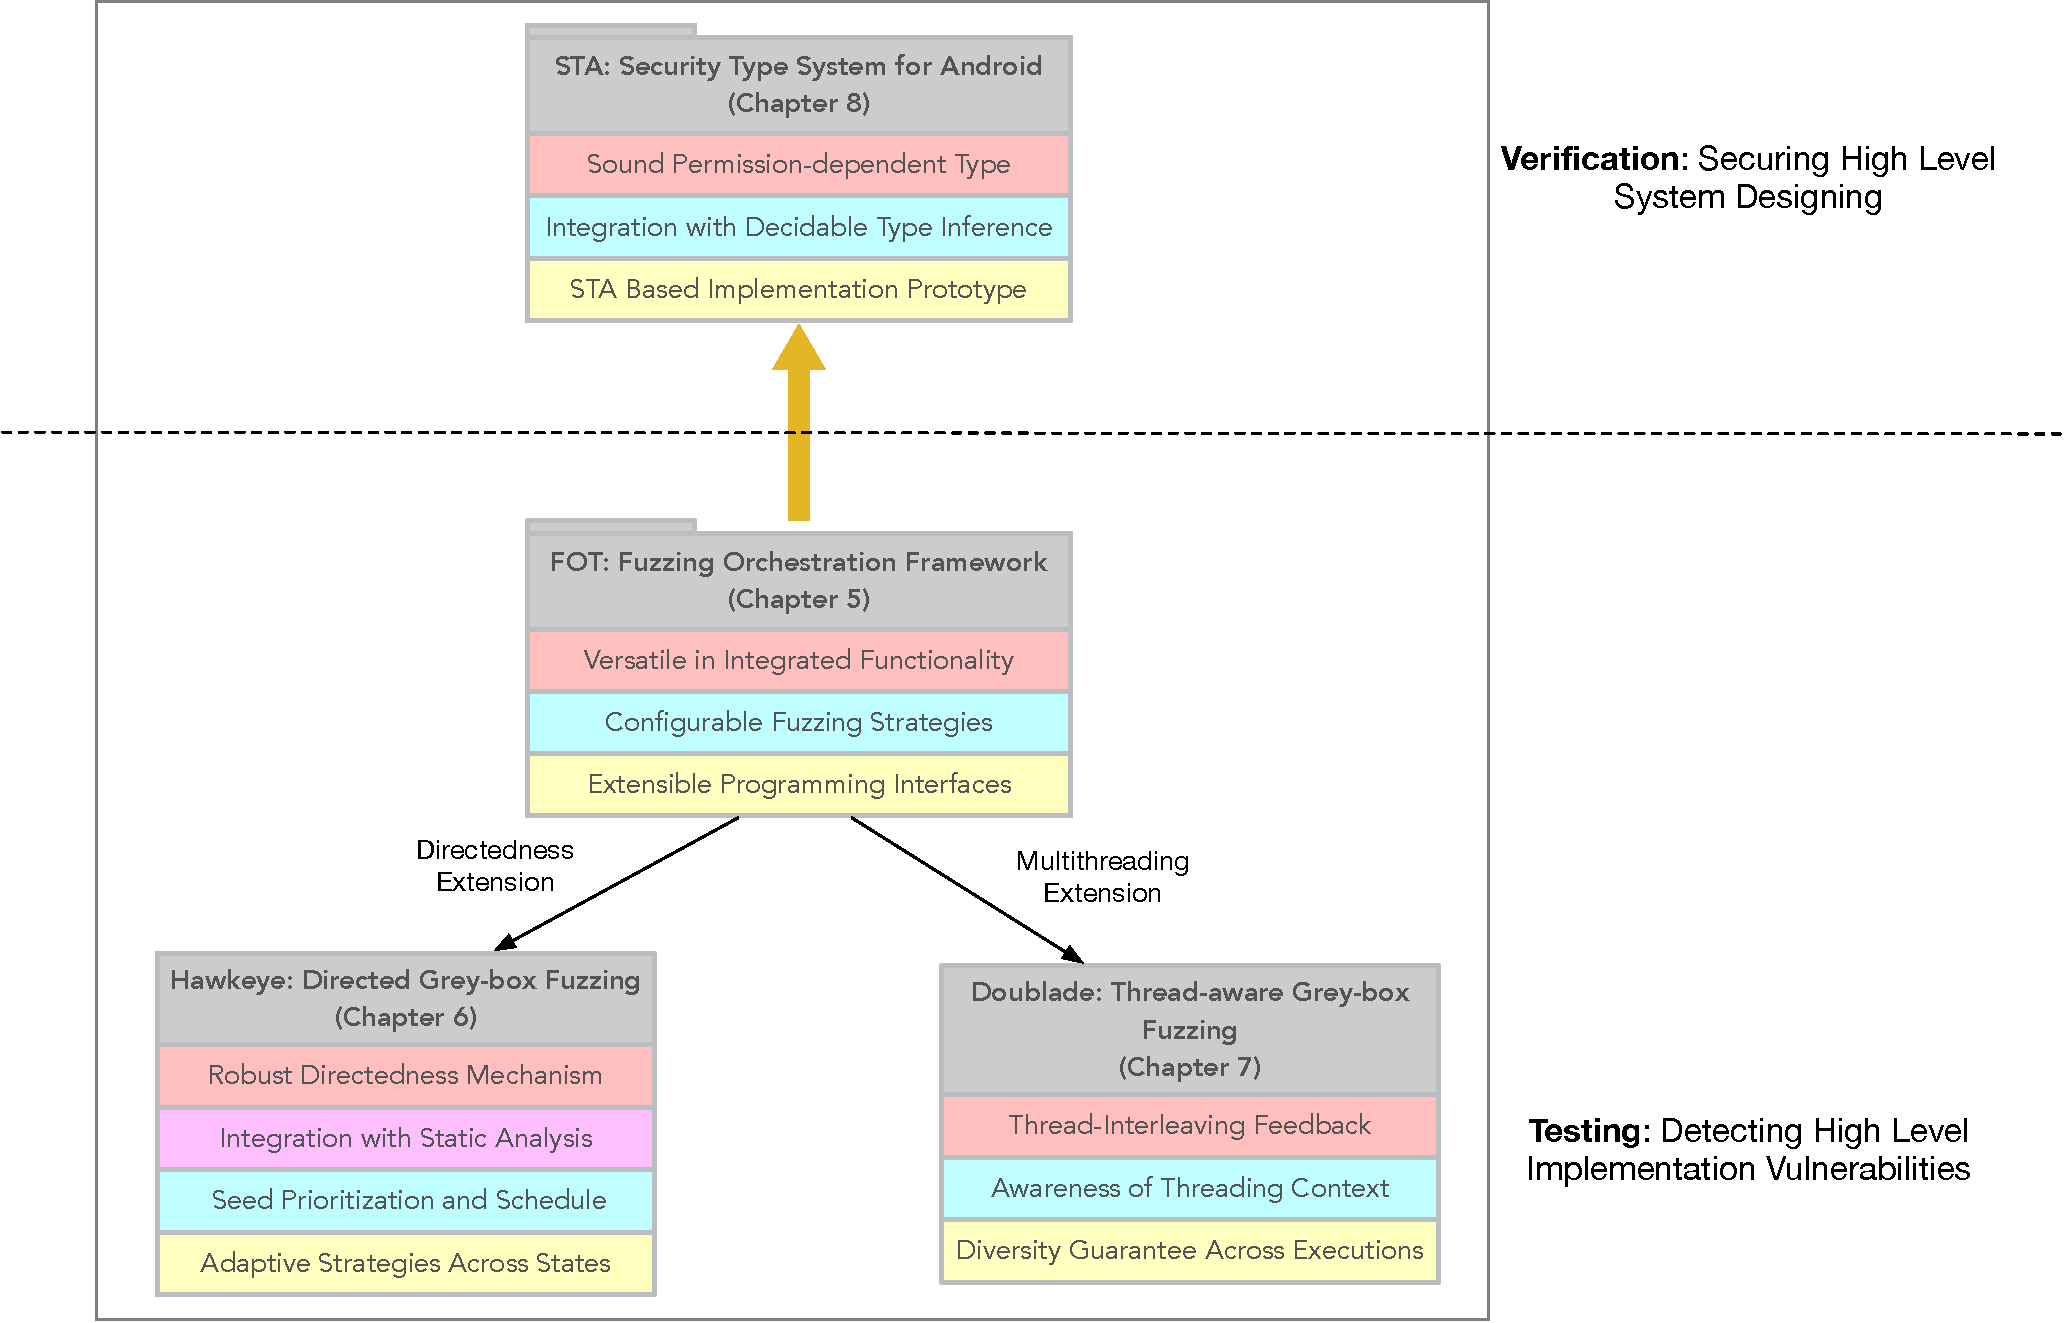
\includegraphics[width=0.9\textwidth]{res/contributions}
		\caption{Main Work of the Thesis and the Relations between its Counterparts}
		\label{fig:works}
	\end{center}
\end{figure}


\section{Main Work}

This work aims to secure the software systems with both \emph{testing} and \emph{verification} approaches. Fig.~\ref{fig:works} depicts the main work of the thesis and their relations.

For testing, we apply the greybox fuzzing approaches to reveal those \emph{implementation induced vulnerabilities}. We firstly build a greybox fuzzing framework called \emph{Fuzzing Orchestration Toolkit}~\cite{fse18-fot}, or \FOT by short. This framework aims to be \emph{versatile}, \emph{configurable}, and \emph{extensible}. It is versatile since it has integrated and will integrate various greybox fuzzing techniques~\cite{Bohme:2016:CGF,Bohme:2017:DGF,redqueen,CollAFL,Angora,fuzz_survey}. It is configurable in that it provides several builtin strategies which allow easy customization for the fuzzing procedure. It is also extensibsle in that it provides fruitful interfaces for easy integration with new techniques. We also apply two novel extensions to \FOT from two aspects. In order to guide the fuzzing procedure to \emph{certain specific program locations}, we propose \dFOT; this can be applied to scenarios such as patching testing, crash reproduction, etc. We pointed out four key properties that are considered important to the guidance: the robust directedness mechanism, the lightweight yet effective integration with static analysis, the optimized seed prioritization and scheduling strategies, as well as the adaptive strategies across fuzzing states. In order to improve the efficiency of fuzzing multi-threaded programs, we propose \mtfuzz, which utilizes the thread-aware analyses to increase the quality of the generated seeds. \mtfuzz provides the thread-interleaving feedback by providing a novel stratified exploration oriented instrumentation, together with the threading context information and the thread scheduling intervention that diversifies the actual interleaving.

Although fuzzing can reveal the implementation specific vulnerabilities, it usually lacks the insight of the higher level design vulnerabilities. For example, although it is possible for fuzz testing to discover multiple crashes in Android core libraries, it usually cannot reveal certain categories of various security issues regarding privacy at the application framework level and the applications built on top of it~\cite{Enck:2009:UAS:1512148.1512324,Ernst:2014}. In fact, it is almost impossible for testing techniques to detect certain security issues in Android due to its designing flaw~\cite{url:android-flaw}. In order to secure the higher level defects such as the information leakage in Android system, we propose a security type system in order to rigorously certify that the underlying system is free of these vulnerabilities. The novelty of the proposed security type system is that we designed a type merging operator that allows for permission-dependent security types. We proved the soundness of the type system in terms of \emph{non-interference}, in which we formally assure no information leakage in the system as long as the security type checking is passed. We also provided a set of type inference rules that are guaranteed to be decidable in finite numbers of steps. In addition, we implemented a prototype of the type system which can type check the information leakage issues in Android.

With these two applied approaches, we aim to provide a comprehensive solution to securing the various software systems such as Linux or Android.

\section{Contributions of the Thesis}
The contributions of the thesis is as follows:
\begin{enumerate}
	\item We provided a greybox fuzzing framework, \FOT, which is versatile in its configurability and extensibility. Based on this, we have integrated several fuzzing techniques and successfully detected more than 200 vulnerabilities in real-world open source programs, among which 51 have been assigned CVE IDs.
	\item We proposed a principled directed greybox fuzzing technique \dFOT to allow for fuzzing on specific program targets and implemented it on top of \FOT. \dFOT innovatively provides the robust directedness mechanism, integrates with a static analysis to calculate the directedness utilities, optimizes the seed prioritization and scheduling, and applies adaptive mutation strategies across different distance states. This effectively improves the fuzzing effectiveness on the given program targets.
	\item We proposed a thread-aware fuzzing technique, \mtfuzz, which significantly improved the effectiveness of fuzzing on multi-threaded programs. \mtfuzz utilizes the thread-aware analysis and applies three categories of instrumentation to explore thread-interleavings,  improve the thread-scheduling diversities across executions, as well as take account of threading context information; based on the feedback provided by the instrumentation, \mtfuzz generates more valuable seeds that can significantly help reveal multithreading relevant vulnerabilities and concurrency bugs.
	\item We provided a permission-dependent type system that precisely enforces access control based on the permission authentication mechanism on Android and proved the soundness of the type system in term of the non-interference property. We also provided a series of decidable type inference rules to assist the type checking. Based on the type system, we implemented a prototype that stresses information leakage issues in Android system.
\end{enumerate}


\section{List of Materials Related to the Thesis}
\begin{enumerate}
	\item \myname, Yuekang Li, Bihuan Chen, Yinxing Xue, Yang Liu, ``FOT: A Versatile, Configurable, Extensible Fuzzing Framework'', ESEC/FSE '18, Proceedings of the 2018 26th ACM Joint Meeting on European Software Engineering Conference and Symposium on the Foundations of Software Engineering, Pages 867-870, \url{http://doi.acm.org/10.1145/3236024.3264593}, DOI: 10.1145/3236024.3264593.
	\item \myname, Yinxing Xue, Yuekang Li, Bihuan Chen, Xiaofei Xie, Xiuheng Wu, Yang Liu, ``Hawkeye: Towards a Desired Directed Greybox Fuzzer'', CCS'18, Proceedings of the 2018 ACM SIGSAC Conference on Computer and Communications Security, Pages 2095-2108, \url{http://doi.acm.org/10.1145/3243734.3243849}, DOI: 10.1145/3243734.3243849.
	\item \myname, Shengjian Guo, Yinxing Xue, Yulei Sui, Cen Zhang, Yuekang Li, Haijun Wang, Yang Liu, ``Doublade: Enhancing Greybox Fuzzing for Multithreaded Programs with Thread-aware Analysis'', submitted.
	\item \myname, Alwen Tiu, Zhiwu Xu, Yang Liu, ``A Permission-Dependent Type System for Secure Information Flow Analysis'', 2018 IEEE 31st Computer Security Foundations Symposium (CSF'18), Oxford, 2018, pp. 218-232. \url{https://doi.org/10.1109/CSF.2018.00023}, DOI: 10.1109/CSF.2018.00023. A technical report is available at \url{https://arxiv.org/abs/1709.09623}.
\end{enumerate}

\section{Outline of the Thesis}

The rest of this thesis is organized as follows.

Chapter~\ref{ch:preliminaries} describes the terminologies and preliminaries throughout this paper. Chapter~\ref{ch:fot} describes the recent progress of fuzzing and several aspects of challenges, and introduces our greybox fuzzing framework, \FOT, which aims to solve these issues. Chapter~\ref{ch:dfot} explains our directed greybox fuzzer \dFOT built on top of \FOT; \dFOT is our attempt to guide the fuzzing process to specific program targets. Chapter~\ref{ch:mtfuzz} describes \mtfuzz based on \FOT, which aims to enhance the fuzzing effectiveness on multithreaded programs. Chapter~\ref{ch:sta} describes our attempt to secure software systems based on verification, which applies a permission-dependent type system to enforce the non-interference property that prevents the information leakage in an Android system. Chapter~\ref{ch:discuss} discusses my reflection on the testing and verification based techniques. Chapter~\ref{ch:conclusion} concludes this thesis and describes the future work.

\fancyhead[RE,LO]{\fancyplain{}{\leftmark}}
\renewcommand{\chaptermark}[1]{\markboth{\chaptername\ \thechapter.\ \emph{Preliminaries}}{}}
\chapter{Preliminaries} \label{ch:preliminaries}

\begin{algorithm}[t]
 \small
\SetKwInOut{Input}{input}
	\SetKwInOut{Output}{output}
	\Input{Program \ProgO, Initial input seeds \Seeds}
	\Output{Final seeds \FinalSeeds, Vulnerable seeds \CrashSeeds}
	\Prog = instrument(\ProgO) \tcp*{instrumentation}
	$\CrashSeeds \leftarrow~\emptyset$, $\FinalSeeds \leftarrow~\Seeds$\; 
	\While {True} {
		$t$ = next\_seed(\FinalSeeds) \tcp*{seed selection}
		\mutChance = get\_mutation\_chance(t) \tcp*{power scheduling} \label{line:algo:energy}
		\For {$i\in~1\ldots \mutChance$} {
			t' = mutated\_input(t)  \tcp*{seed mutation}
			res = run(\Prog, t', \Ncal)\tcp*{calibration execution}
			\uIf {is\_crash(res)}{\label{line:algo:triage_start}
				$\CrashSeeds = \CrashSeeds\cup\{t'\}$ \tcp*{report vulnerable seeds}
			}\ElseIf {cov\_new\_trace(t', res)} {\label{line:algo:new_cov}
				$\FinalSeeds = \FinalSeeds\cup\{t'\}$ \tcp*{save "good" seeds} \label{line:algo:triage_end}
			}
		}
	}
	\caption{Greybox Fuzzing}\label{algo:gbf}
\end{algorithm}

In this chapter, we briefly describes some terminologies and preliminaries used throughout the thesis.

\section{Greybox Fuzz Testing}\label{sec:intro-gbf}
Since its introduction in the early 1990s~\cite{fuzzing1990}, \emph{fuzz testing}, or \emph{fuzzing}, has remained highly popular due to its conceptual simplicity, its low barrier to deployment, and its vast amount of empirical evidence in discovering real-world software vulnerabilities~\cite{fuzz_survey}.

Greybox fuzzers (GBFs), which apply some instrumentations and utilize the collected dynamic statistics as feedback to guide the fuzzing procedure, have been proven to be effective in generating seeds and detecting vulnerabilities in modern programs~\cite{fuzz_survey}. Specially, AFL~\cite{afl}, libFuzzer~\cite{libfuzzer}, honggfuzz~\cite{honggfuzz} and the fuzzing infrastructure ClusterFuzz~\cite{clusterfuzz} have been able to detect more than 16,000 vulnerabilities or bugs in over 160 open source projects~\cite{afl,clusterfuzz}. Greybox fuzzing strikes a balance between mutation effectiveness and it execution speed. Compared to blackbox fuzzing, greybox fuzzing at some extent knows about the target program under test via the instrumentation, therefore it has the capability to effectively guides the fuzzing procedure to much more valuable paths. Compared to white-box fuzzing techniques such as symbolic execution~\cite{dart,klee}, it is extremely lightweight and far more scalable to real-world projects.


Algo.~\ref{algo:gbf} presents the core procedures of a typical greybox fuzzing algorithm. Basically, it involves an instrumentation step and a fuzzing loop.

Given a target program \ProgO and input seeds \Seeds, a GBF first applies the instrumentation to track the coverage information in \ProgO. That is, the actual PUT is \Prog. In spite of the difference, since the instrumentation typically does not significantly change the regular flow of a program's semantics, the crash on \Prog usually still indicates a weakness inside \ProgO. In practice, this difference is usually neglected.
The instrumentation can be done statically or dynamically. Static source instrumentation is usually applied during the source compilation procedure, with the help of compilation infrastructure such as LLVM~\cite{Lattner:2004:LCF:977395.977673}, GCC~\cite{gcc}. Dynamic binary instrumentation (DBI) is done with the help of DBI frameworks such as Valgrind~\cite{valgrind}, Intel PIN~\cite{pin}. Logically, instrumentation does not belong to fuzzing procedure, and its purpose is to collect feedback during fuzzing. Usually, the instrumentation does not involve deep static analyses.


The fuzzing loop does the actual mutations and testings against the program.
\begin{enumerate}[1.]
	\item Based on the seed priority, \emph{seed selection} selects next candidate seed $t$ from the queue which is formed by \Seeds.
	\item \emph{Seed mutation} procedure determines based on previous execution statistics on $t$ to determine how many mutation chances (\mutChance) will be provided for $t$.
	\item It enters the \emph{monitored execution} against the variants of $t$ with \mutChance iterations. 
	\begin{enumerate}[a)]
	\item Firstly, it applies \emph{seed mutation} on $t$ to generate a seed $t'$. 
	\item Secondly, it goes to the actual \emph{calibration execution} against $t'$; for statistics collection purpose, the fuzzer usually executes \Prog against $t'$ with continuously $\Ncal$ times. This is due to the fact that a single run on a specific seed may not be stable and the fuzzer needs to collect \emph{average statistics} for further scheduling.
	\item Finally, the fuzzer handles the generated seeds based on the execution results: the vulnerable seeds will be reported and those that are considered ``good'' according to the feedback will be appended to the seed queue for subsequent mutations.
	\end{enumerate}
\end{enumerate}
As the fuzzer's awareness of the program structure is based on the instrumentation feedback, a GBF typically does not \emph{know} the PUT itself; therefore it usually has no idea when to stop the fuzzing procedure. In practice, the fuzzing procedure is terminated manually.

In the recent years, many approaches have been proposed to increase the fuzzing effectiveness in different aspects~\cite{Bohme:2016:CGF,LiCMLLT17,Bohme:2017:DGF,FairFuzz,CollAFL,Angora,nezha,fuzz_survey}. For example, Angora~\cite{Angora} proposes to introduce fine-grained instrumentation and applies constraint solving to increase coverages; Coll-AFL~\cite{CollAFL} proposes a path sensitive approach to avoid collisions; Skyfire~\cite{junjie:2017sp:skyfire} attempts to improve the mutation operations on structure-sensitive programs. These have lead to further advances in the greybox fuzzing.

\section{Security Type Checking on Android}\label{sec:intro-sta}

\subsection{Language-based Type Checking on Information Flow}

The starting point of security type checking based verification is the classification of program variables into different security labels. The simplest is to classify some variables as $L$, meaning low security (public), while other variables as $H$, meaning high security (private). The goal is to prevent private information variables from being leaked publicly, i.e., prevent information in $H$ variables from \emph{flowing} to $L$ variables.

As to \emph{confidentiality}, the common practice is to treat the set of the security labels as a  \emph{lattice} and the information flows only upwards in the lattice~\cite{Denning:1977hwa}. For example, since $L\leq H$, we would allow flows from $L$ to $L$, from $H$ to $H$, and from $L$ to $H$, but we would disallow flows from $H$ to $L$.

Below is an example taken from Denning~\cite{Denning:1976cl}. We assume \textsf{secret}$:H$ and \textsf{leak}$:L$, and the attacker can observe any variable at level $L$ but no variable at $H$.
From the confidentiality requirement, $\textsf{leak:=secret}$ is illegal while the assignment $\textsf{secret:=leak}$ works fine. This is due to the fact in the former case the secret information may be observed by the attacker when he/she sees the value of \textsf{leak}, which has the same value as \textsf{secret} after the assignment and is accessible by the attacker who has observation level not less than $L$. The leak is caused by an explicit data flow and is so-called \emph{explicit flow}. On the other hand, control flow can also leads to \emph{implicit flow} leaks. For example,
\begin{lstlisting}[language=c,float=h]
if ((secret mod 2) == 0) {
  leak := 0;
} else {
  leak := 1;	
}  
\end{lstlisting}

Despite that the \textsf{if-else} construct is not intended for data transfer, this segment is essentially equivalent to $\textsf{leak:=secret}$, which obviously violates the confidentiality. Therefore this is as dangerous as the direct assignment.

Some complex data structures may result in subtle information leaks. For example, if array \textsf{a} is initialized with all \textsf{0}s, then the program below is still leaking information due to the fact that after the execution, \textsf{leak} will be assigned to \textsf{i}, which is still the value of \textsf{secret}. There is also a leak from \textsf{secret} to \textsf{leak}.

\begin{lstlisting}[language=c,float=h]
a[secret] := 1;
for (int i := 0; i < a.length; i++) {
  if (a[i] == 1) leak := i;
}
\end{lstlisting}

\subsubsection{Non-interference}
At a program level, the security properties are described as \emph{non-interference}, which was described by Goguen and Meseguer in 1982~\cite{Goguen:1982ta}. The simplest form tells that a deterministic program $c$ satisfies non-interference, if and only if, for any memories $\mu$ and $\nu$ that agree on $L$ variables, the memories produced by running $c$ on $\mu$ and on $\nu$ also agree on $L$ variables (provided that both terminate successfully). Basically, the program can be viewed as a state machine. If a low user is working on the machine, it will respond in exactly the same manner (on the low outputs) whether or not a high user is working with sensitive data. The low user will not be able to acquire any information about the activities (if any) of the high user by observing the values of low variables.

Typically, a security type system is introduced to prove the non-interference property. In addition to the regular types (such as integer, boolean, etc.), expressions and commands also contain security labels. And by applying the well-established typing derivation approach, it is fairly enough by reasoning over provided typing rules to verify the property, thus it provides a certificate to the underlying program.

The non-interference property can also be applied to more complex systems when covert channels are considered. Implicit (control) flow can be seamlessly integrated into the typing rules by security typing on branching constructs. In fact, almost all security type systems handle implicit flows. Termination channels, which signal information through the termination or nontermination of a computation, can be handled by a revised termination-sensitive non-interference definition. Timing channels, probabilistic channels, resource exhaustion channels, and power channels, can also be encoded in a type system in order to preserve an adapted non-interference property.

\subsubsection{Typing Principles}

When applying type systems to guard information flows, a security label is typically associated with security type $\tau$ apart from the regular data type. The goal is to prove the soundness of the type system; that is, the problem survives the required security properties as long as it is well-typed in terms of the security types.

In Bell-Lapadula Model~\cite{bell1973}, it requires the subject at a given level must not write to any object at a lower security labels, and not read any object a higher security labels, which is characterized by the phrase ``no read up, no write down'', and it is safe to treat data that is low confidential to be high. In term of language based secure type systems, this is termed as \emph{Simple Security} and \emph{Confinement Security}. The former applies to expressions and later applies to commands. If an expression $e$ can be given type $\tau$ in the system, then Simple Security says, for secrecy, that only variables at level $\tau$ or lower in $e$ will have their contents accessed (read) when $e$ is evaluated (``no read up''). On the other hand, if a command $c$ can be given type $\tau$, then Confinement says, for secrecy, that no variable below level $\tau$ is updated (modified, writen) in $c$ (``no write down'').

The concrete security typing rules vary in the underlying type systems to guarantee these two properties. However, normally two subsumption rules are present in addition to the syntax-directed typing rules. That is, for expressions, it follows a co-variant view(\ruleTagText{Sub$_e$}); and for commands, it follows a contra-variant view(\ruleTagText{Sub$_c$}).

\begin{equation*}
\inference
{e:\tau & \tau\leq\tau'}
{e:\tau'}
\ruleTagMath{Sub$_e$}
\qquad
\inference
{c:\tau & \tau'\leq\tau}
{c:\tau'}
\ruleTagMath{Sub$_c$}
\end{equation*}

Intuitively, \ruleTagText{(Sub$_e$)} depicts the fact that it is always safe to read less confidential data as more confidential one; while \ruleTagText{(Sub$_c$)} discloses that if there is no variable below level $\tau$ updated in $c$, then there is surely no variable below $\tau'$ updated in $c$, as long as $\tau'\leq\tau$.

\subsection{Android Security Model}
The security model of Android system differs significantly from standard security models such as regular Bell-La Padula, mandatory access control (MAC), etc. In fact, Android applications (or apps for short) are treated as mutually distrusting principals: they are isolated from each other and do not have access to the others' private (local) data. The mechanism is achieved by Android discretionary access control (DAC), which originates from Linux's access control mechanism. Next, we provide an overview of Android security model and its inter process communication (IPC) facilities.

\subsubsection{Thread Model}

The Android Market contains a large number of third-party apps, and a user may install apps with different trust levels. Users install apps from unknown developers alongside trusted apps that handle private information such as financial data and personal photographs. For example, a user might install both a highly trusted payment app, as well as a free game app. In most of the scenarios, the user would not expect that the game app has access to the user's payment information.

Under Android security model, all the apps are treated as potentially malicious. Each app runs in its own process with a low-privilege user ID, and apps can only access their own files by default. This isolation mechanism aims to protect apps with sensitive information from malware. Despite that, apps can inherently communicate via message passing (which is by convention called inter-process/app communication, IPC), which has been and is being utilized by various malware. In fact, the app might leak sensitive data, whenever the app sends information to the recipient without proper permission checking on the latter.

\subsubsection{App Components and IPC Mechanism}

Intents are logical app building blocks delivered to app components. There are four categories of components in Android:

\begin{description}
	\item[Activity] components form the basis of the user interface. Typically, each activity corresponds to certain ``window'' in the underlying app.
	\item[Service] components run as a daemon, and remain active even if the windows are switched. Services can expose interfaces for communication with other apps.
	\item[BroadcastReceiver] components react asynchronously to messages from other apps.
	\item[ContentProvider] components store app's data, usually in a database. Such data may sometimes be allowed to be shared across different apps.
\end{description}

In particular, \emph{intents} are frequently used for message passing within or across apps. An intent is an abstract description of an operation to be performed. It is a message that declares a recipient, optionally with data. An intent can be thought of as a self-contained object that specifies a remote procedure to invoke/call and includes the associated arguments (remote procedure call, RPC). Intents are widely used for both inter-app communication and intra-app communication.

Intents can be sent between three of the aforementioned four components: Activities, Services, and Broadcast Receivers. They can be used for different purposes, such as starting Activities, starting, stopping, and binding Services, broadcasting information to BroadcastReceivers, etc. All of these communications can be used with explicit or implicit Intents. A component receives only internal app Intents defautly.

Intents can be used for explicit or implicit communication. An explicit intent regulates that it should be delivered to a particular app with explicit app ID, whereas an implicit intent requests delivery to any app that satisfies certain properties. In other words, an explicit intent identifies the intended recipient by name, whereas an implicit intent's recipient(s) are eventually determined by the Android system based on the recipient's/recipients' support for certain operations. For example, consider an app that stores contact information. When a user clicks on one of his or her contacts' family address, the ``contacts app'' needs to ask another app to display a map of that location (in Android, it would be a \textsf{ACTION\_VIEW} action with the data URI of the scheme ``\textsf{geo:0,0?q=my+street+address}''). In this scenario, the contacts app could send an \emph{explicit intent} directly to Google Maps (in most cases, it is enough to call \textsf{intent.setPackage("com.google.android.apps.maps")} followed by a \textsf{startActivity(intent)}). Alternatively, it could also send an \emph{implicit intent} that would be delivered to any app that says it provides mapping functionality such as Yahoo! Maps (e.g., only \textsf{startActivity(intent)} is called). Using an explicit intent guarantees that it is delivered to the intended recipient, whereas implicit Intents allow for late runtime binding between different apps. {Typically, the resolution result is checked by calling of \textsf{intent.resolveActivity(getPackageManager())}, which is unknown until runtime.}

\fancyhead[RE,LO]{\fancyplain{}{\leftmark}}
\renewcommand{\chaptermark}[1]{\markboth{\chaptername\ \thechapter.\ \emph{\dFOT: Directed Greybox Fuzzing}}{}}
% !TeX root =../../main.tex

\chapter{\dFOT: Directed Greybox Fuzzing} \label{ch:dfot}


\section{Introduction and Motivation}


Generally speaking, existing greybox fuzzers aim to cover as many program paths as possible within a limited time budget.
However, there exist several testing scenarios where the programmers only care about certain specific paths or locations and hope these can be sufficiently tested. 
For example, if \emph{MJS}~\cite{mjs} (a JavaScript engine for embedded devices) has a vulnerability discovered on MSP432 ARM platform, similar vulnerabilities may occur in the corresponding code for the other platforms.
In such a situation, the fuzzer should be \emph{directed} to reproduce the bug at these locations.
In another scenario, the programmers need to check whether a given patch indeed fixes the bug(s) in the previous versions~\cite{ase18:cldiff,SemSlice,fse16:bingo,usec20:HotPatch}. 
This requires the fuzzer to concentrate on those locations that are affected by patched code.
In both scenarios, the fuzzer is expected to be directed to reach certain user specified locations in the target program.
For clarity, we name such locations as \emph{target locations}.
Following the definition in {\aflgo}~\cite{Bohme:2017:DGF}, we name those fuzzers that can fulfill the directed fuzzing task as \emph{directed fuzzers}.


{\aflgo}~\cite{Bohme:2017:DGF} is a variant of the state-of-the-art fuzzer AFL. It is a directed greybox fuzzer (DGF) that reduces the reachability of target locations to an \emph{optimization problem}. It adopts a meta-heuristic to promote the  seeds with shorter distances. The distance is calculated based on the average the \emph{weight} of basicblocks on seed's execution trace to the target basicblock(s), where the weight
 is determined by the edges in the call graph and control flow graphs of the program, and the applied meta-heuristic is simulated annealing~\cite{kirkpatrick1983optimization}.
Owing to these, \aflgo improves the \emph{power scheduling} for fuzzing directedness --- how many new seeds (a.k.a. ``energy'' in \aflgo) should be generated from the current seed.
%DGF achieves the goal of reaching the target locations by \emph{combing both static analysis and dynamic analysis}.

A pure dynamic execution can only get the feedback based on the traces it has \emph{already} covered without any awareness about the predefined target locations.
Thus, \textbf{\emph{static analysis}} is required to extract the necessary information for guiding the execution towards the target locations for DGFs. The most widely adopted is to calculate the \emph{distance} to the target locations for the components (e.g., basicblocks, functions) of the target program, so that when executed, DGFs can decide the \emph{affinity} between current seed and the target locations from the components in the execution traces. 
The major challenge is that the distance needs to be efficiently calculated while not compromise certain desired features.
In particular, it should help to keep to some extent the seed diversity~\cite{Audibert09}.
For example, the existing seed distance calculation algorithm used in \aflgo always favors shortest path that leads to the target locations (see \S~\ref{subsec:motiv}), which may starve seeds that could be more easily mutated to reach the target location and further trigger crashes.
The author of libFuzzer~\cite{libfuzzer} argues that not taking into account \emph{all the possible traces} may fail to expose the bugs hidden deeply in longer paths~\cite{kcc_aflgo}.
This derives the first desired property \textbf{P1}.
Another challenge is that the static analysis should provide precise information with acceptable overheads.
This is because that coarse static analyses will not benefit the dynamic fuzzing much, while \emph{heavyweight static analyses themselves may take considerable time} before the dynamic fuzzing starts.
This challenge derives the second desired property \textbf{P2}.
Therefore, the first issue is \emph{how a DGF applies proper static analysis effectively and efficiently to collect necessary metrics}.

After static analysis, there are several  challenges in \textbf{\emph{dynamic analysis}} --- how to dynamically adjust different strategies for the purpose of reaching the target locations as fast as possible.
The first challenge is how to properly \emph{allocate energy} to the seeds with different distances and how to \emph{prioritize} the seeds closer to the target locations.
This derives the third desired property \textbf{P3}.
The second challenge is how to adaptively change the mutation strategies, since GBFs may possess various mutation operators at both coarse-grained (e.g., chunk replacement) and fine-grained (e.g., bitwise/bytewise flip) levels.
 This derives the fourth desired property \textbf{P4}.
Therefore, the second issue is \emph{how a DGF applies adaptive strategies during the dynamic fuzzing procedure}.


To emphasize the two aforementioned issues, we suggest that an ideal DGF is expected to hold the following desired properties (\S\ref{subsec:dp}):
\begin{enumerate}[\textbf{P}1]
\itemsep0em 
\item It should provide a \emph{robust} mechanism guiding the directed fuzzing by considering all the possible traces to the target locations.
\item It should strike a \emph{balance} between utilities and overheads as to static analysis.
\item It should prioritize and schedule the seeds to reach target locations \emph{rapidly}.
\item It should adopt an \emph{adaptive} mutation strategy across different program states.
\end{enumerate}


We propose our solutions to achieve the 4 properties for DGF. 
For \textbf{P1}, we propose to apply the static analysis results to augment the adjacent-function distance (\S\ref{subsec:functionDist}); and the function level distance and basicblock level distance should be calculated based on the augmented adjacent-function distance to simulate the affinities between functions (\S\ref{subsec:UtilityComputation}).
Meanwhile, during fuzzing, we calculate \emph{basicblock trace distance} and \emph{covered function similarity} of the execution trace to that of the target functions (\S\ref{subsec:powerSche}) by integrating the static analysis results with the runtime execution information.
For \textbf{P2}, we propose to apply the analysis based on call graph (CG) and control flow graph (CFG), i.e., the function level reachability analysis, the points-to analysis for function pointers (indirect calls), and the basicblock metrics (\S\ref{subsec:graghCons}). 
For \textbf{P3}, we propose to combine the basicblock trace distance and covered function similarity for solving the power scheduling problem (\S\ref{subsec:powerSche}) and the seed priorization problem (\S\ref{subsec:prioritization}). 
For \textbf{P4}, we propose to apply an adaptive mutation strategy according to the reachability analysis and covered function similarity~(\S\ref{subsec:mutationStr}).

By taking these properties into account, we implemented our DGF, {\dFOT}, and conducted a thorough evaluation with various real-world programs. 
The experimental results show that in most cases, {\dFOT} outperforms the state-of-the-art greybox fuzzers in terms of the time to reach the target locations and the time to expose the crashes.
Particularly, {\dFOT} can expose certain crashes up to 7 times faster than the state-of-the-art \aflgo, reducing the time to exposure from 3.5 hours to 0.5 hours.

In practice, \dFOT has been successfully discovering crashes with the suspicious target locations reported by other vulnerability detection tools and successfully found more than 41 previously unknown crashes in projects Oniguruma~\cite{oniguruma}, MJS\cite{mjs}, etc. All these vulnerabilities have been confirmed and fixed; among them, 15 vulnerabilities have been assigned unique CVE IDs.

The main contributions of this chapter are summarized as follows:
\begin{enumerate}[1)] 
\itemsep0em
\item We analyzed the challenges in directed greybox fuzzing and summarized the four desired properties for DGFs.
\item We provided a measure of power function that can guide the fuzzer towards the target locations effectively.
\item We proposed a novel approach to boost the convergence speed to the target locations by utilizing power scheduling, adaptive mutation and seed prioritization.
\item We implemented \dFOT that organically combines these ideas and thoroughly evaluated our results in crash reproduction and target location covering.
\end{enumerate} 

\section{Desired Properties of DGF}\label{sec:mx}

In this section, we first show an example to illustrate the difficulties in DGF.
Based on the observations from the example,~we then propose four desired properties for an ideal DGF.
Finally, we review the state-of-the-art DGF, namely \aflgo~\cite{Bohme:2017:DGF}, with respect~to these four desired properties. 


\subsection{Motivating Example}\label{subsec:motiv}



Figure~\ref{fig:exam_trace} shows two execution traces related to CVE-2017-15939~\cite{cve-2017-15939}, which is a NULL pointer dereference bug caused by~an incomplete fix in CVE-2017-15023~\cite{cve_2017_15023}.
This vulnerability is difficult for~the~existing GBFs to discover.
For instance, AFL~\cite{afl} fails to detect this vulnerability within 24 hours in all the 10 different runs we conducted.
This bug is triggered in \texttt{nm} from GNU binutils.
In function \texttt{concat\_filename}, a NULL pointer is assigned and used without checking, which triggers the segmentation fault.
From a patch testing perspective, we would like to target \texttt{concat\_filename} (subsequently, we will denote this as $T$) and guide the fuzzing to reproduce the crashing trace (i.e., $\langle a, b, c, d, T, Z\rangle$ in Figure~\ref{fig:call_chain}).




\begin{figure}[t]
	\centering
	\myeqsize \begin{tabular}{lcc}
		\hline
  \textbf{Functions in a Crashing Trace} &  	\textbf{File \& Line} & \textbf{Symbol} \\\hline
  	 \texttt{main}   &   \texttt{nm.c} :1794     & \textsf{$M$}\\
 	   ... &  ...  &...  \\
 	 \texttt{\_bfd\_dwarf2\_find\_nearest\_line}     &   \texttt{dwarf2.c} :4798   &  \textsf{$a$}\\
 	 \texttt{comp\_unit\_find\_line}    &   \texttt{dwarf2.c} :3686    & \textsf{$b$}\\
 	 \texttt{comp\_unit\_maybe\_decode\_line\_info} &	 \texttt{dwarf2.c} :3651       &  \textsf{$c$}\\
  	 \texttt{decode\_line\_info}   &    \texttt{dwarf2.c} :2265     &  \textsf{$d$} \\
\texttt{concat\_filename}   &   \texttt{dwarf2.c} :1601     &  \textsf{$T$}\\
    ... 	 	  &     ... 	  &  \textsf{$Z$}\\\hline
	  \textbf{Functions in a Normal Trace} &  	\textbf{File \& Line} & \textbf{Symbol} \\\hline
	   \texttt{main}   &   \texttt{nm.c} :1794     &  \textsf{$M$}\\
	      ... &  ...  &...  \\
	   \texttt{\_bfd\_dwarf2\_find\_nearest\_line}     & \texttt{dwarf2.c} :4798      & \textsf{$a$}\\
	  \texttt{scan\_unit\_for\_symbols}    &      \texttt{dwarf2.c} :3211        &  \textsf{$e$}\\
  \texttt{concat\_filename}   &  \texttt{dwarf2.c} :1601      &  \textsf{$T$}\\
	    ... 	 	  &     ...       & \textsf{$Z$}\\\hline
	\end{tabular}
\vspace{-5pt}
	\caption{Two execution traces relevant with CVE-2017-15939, where $M$ is the entry function, $T$ is the target function, and $Z$ is the exit.}
	\label{fig:exam_trace}
\end{figure}



For simplicity, in Figure~\ref{fig:call_chain}, we illustrate only three representative traces for the CVE-2017-15939 by omitting 1) the overlapping functions before $a$ and 2) the other traces that do not pass the target function $T$. {The difficulty in discovering this CVE for the general GBFs (e.g., AFL) arises from the fact that the target function $T$ is deeply hidden in the crashing trace.} As shown in Figure~\ref{fig:call_chain}, the call chain of $\langle a, e, T, Z\rangle$ is shorter than $\langle a, b, c, d, T, Z\rangle$.

Since most of the GBFs (such as AFL, LibFuzzer, etc.) are supposed to be \emph{coverage oriented}, and do not care specially about the target locations, they may not put most of their efforts in generating seeds that reach function $T$ and testing the function throughly. For DGFs, although there suppose to be some efforts to guide the fuzzing procedure to favor \emph{some} traces leading to $T$ and focus more on these traces, they may frequently miss \emph{all} the traces. For example, if \aflgo detects that two traces can reach the target locations, it will highly likely favors the trace with shorter path: the distance between the seed to the target is determined by the average distance of the components (basicblocks or functions) in the execution trace to the target locations, where the components' distance to the target locations are essentially determined by the number of edges between the components and the target locations. This mechanism causes \aflgo to give more energy to the trace $\langle a, e, T, Z\rangle$ since it reaches the target $T$ \emph{and} the induced trace distance is smaller than $\langle a, b, c, d, T, Z\rangle$; on the other hand, less attention is put on $\langle a, b, c, d, T, Z\rangle$, which however causes the crash under some circumstances. Worse still, other traces like $\langle a, e, f, Z\rangle$ may be mistakenly assigned with more energy. As a result, \aflgo was also not able to reproduce the crash within 24 hours in any of the 10 runs we conducted.
 
The challenges of the existing DGF roots in the following aspects: 1) the target functions may appear in several places in target program, and multiple different traces may lead to the target.  2) since the call graph majorly affects the calculation of the trace distance (the dissimilarity with the target locations), it needs to be accurately built;
in particular, the indirect calls among functions should not be ignored. If the above two issues are not well handled, the distance-based guiding mechanism for DGF will get hindered and fail in such cases.


\subsection{Desired Properties of Directed Fuzzing} \label{subsec:dp}

We observe that an ideal DGF should possess the following desired properties.

\begin{figure}[t]
	\centering
	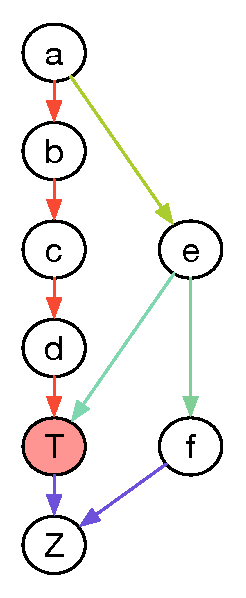
\includegraphics[width=0.11\columnwidth]{res/dfot/eg_callchain.pdf}
	\vspace{-5pt}
	\caption{Fuzzing traces for Figure~\ref{fig:exam_trace}: $\langle a, b, c, d, T, Z\rangle $ is a crashing trace passing $T$,  $\langle a, e, T, Z\rangle$ is a normal trace passing $T$; $\langle a, e, f , Z\rangle$ does not pass $T$.}
	\label{fig:call_chain}
\end{figure}

\textbf{P1. DGF should define a \emph{robust} distance mechanism to guide directed fuzzing by avoiding the bias to certain traces}  \label{subsec:p1}
Different from general GBFs, to reach the specified locations, there may exist several execution traces towards them. More often than not, a target function could appear several times in the code and be called even from different entries of the code. Without any static information as guidance, during the fuzzing process, the fuzzer knows nothing about the execution traces that cover the target locations before they have been executed; and even if the locations have already been covered, the fuzzer does not know whether there are \emph{other} traces that can lead to them.  
Taking Figure~\ref{fig:call_chain} as an example, in the AFL fuzzing process, trace $\langle a, b, c, d, T, Z\rangle$  may not be ever exercised by the existing seeds due to the existence of a strong precondition before $a$. Therefore, \emph{the guiding mechanism should provide the knowledge of all the possible traces that lead to the target locations and guide the mutation towards it via gradually reducing the distance}. 

However, for DGF, awareness of all the possible traces towards target locations is not enough: the distance to specified locations for all traces should be properly calculated so that all traces reachable to them will be assigned more energy compared to other traces. For Figure~\ref{fig:call_chain}, $T$ is the target and we would like to check the functionality of $T$. Note that if we know in advance that \emph{only} the traces that involve $d$ and $T$ may cause crashes, we can set \emph{both} $d$ and $T$ as target locations. Intuitively, traces $ \langle a, e, T, Z\rangle$ and $\langle a, b, c, d, T, Z\rangle$ should be treated without bias as both of them can lead to the target location, while $ \langle a, e, f , Z\rangle$ should be less important as it misses the target location. 



\textbf{P2. DGF should strike a \emph{balance} between efficiency and effectiveness for static analysis.}
Effective static analysis can benefit the dynamic fuzzing procedure in two aspects: 1) In real-world C/C++ programs, there are indirect function calls (e.g., passing a function pointer as a parameter in C, or using function objects and pointers to member functions in C++). In the presence of indirect calls, call sites cannot be observed directly from the source code or binary instructions. So the trade-offs between overheads and utilities need to be made for analyzing them. 2) Not all call relations should be treated equally. For example, some functions occur multiple times in its calling functions, implying  that they have higher chance to be called at runtime. From the static analysis perspective, we need to provide a way to distinguish these scenarios. As to function level distances between functions that have \emph{immediate} calling relations, it is intuitive that callees called in multiple times in different branches should be ``closer'' to the caller.


To sum up, taking Figure~\ref{fig:call_chain} as an example, \emph{the desired design} for the DGF is: 1) if function $a$ (transitively) calls $T$ in an indirect way (i.e., one or more calls in the chain $a\rightarrow\! b\!\rightarrow\! c\!\rightarrow\! d\!\rightarrow\! T$ are through function pointers), the static analysis should capture such indirect calls, otherwise the distance from $a$ to $T$ will be not available (i.e., treated as unreachable). 2) if the callee appears in more different branches and occurs more times in its caller, a smaller distance should be given since it may have more chance of being called for reaching the target(s). However, modeling the \emph{actual} branch conditions in static phrase is impractical due to the inherent limitations of static analysis. For example, given a nontrivial code segment, it is hard to predict whether the true branch of a predicate will be executed more often than its false branch during runtime. On the other hand, tracking symbolic conditions \emph{dynamically} would be too time costly in a greybox fuzzing setting.

\textbf{P3. DGF should \emph{prioritize} seeds close to target locations.}
 AFL determines how many new seeds should be generated (i.e., ``energy'') from a seed to improve the fuzzing effectiveness (i.e., increase the coverage); this is termed ``power scheduling'' in~\cite{Bohme:2016:CGF,Bohme:2017:DGF}. In directed fuzzing, the goal of fuzzing is not to reach \emph{the upper-limit of coverage} as fast as possible, but reach the \emph{particular target locations} as fast as possible. Hence, power scheduling in DGF should determine how many new seeds should be generated from a seed in order to get a new seed that leads to the target locations~\cite{Bohme:2017:DGF}. Similarly, the seed prioritization in DGF is to determine an optimized fuzzing order of seeds to reach target locations as fast as possible. Both of them can be guided by the distance-based mechanism which measures the affinity between the current seed to the target locations. 
 
 For \emph{power scheduling}, the desired design is that the seed trace with a smaller distance to the target locations should be assigned more energy for fuzzing, as the trace closer to the target locations gets better chance to reach there. Therefore, $\langle a, e, T, Z\rangle$ should be allocated with similar energy with $\langle a, b, c, d, T, Z\rangle$, and $\langle a, e, f, Z\rangle$ should have less energy than the previous two. For \emph{seed prioritization}, seeds that have smaller distance (``closer'') to the target locations should be fuzzed earlier in subsequent mutations. Therefore, $\langle a, e, T, Z\rangle$ and $\langle a, b, c, d, T, Z\rangle$ should be put ahead of $\langle a, e, f, Z\rangle$.

\textbf{P4. DGF should adopt an \emph{adaptive} mutation strategy at different program states.}  \label{subsec:p4}
 GBFs usually apply different mutations, such as bitwise flip, byte rewrite, chunk replacement, to generate new seeds from the existing one. 
In general, these mutators can be categorized into two levels: fine-grained mutations (e.g., bitwise flip) and coarse-grained mutations (e.g., chunk replacement).
 Although there is no direct evidence that fine-grained mutations will likely preserve the execution traces, it is widely accepted that a coarse-grained random mutation has a high chance to greatly change the execution trace. Therefore, the desired design is that when a seed has already reached the target locations (including target lines, basicblocks or functions), it should be given less chances for coarse-grained mutations.
 
For the example in Figure~\ref{fig:call_chain}, consider the case where the DGF has already reached the target function via trace $\langle a, b, c, d, T, Z\rangle $, but crash is not triggered yet.
Now, the DGF should allocate less chances for coarse-grained mutations for the input of $\langle a, b, c, d, T, Z\rangle $.
Meanwhile, if DGF has just started up and $\langle a, b, c, d, T, Z\rangle $ has not been reached yet, the DGF should give more chances for coarse-grained mutations.



\subsection{AFLGo's Solution} \label{subsec:aflgo_sol}


In this section, we evaluate the solution of \aflgo against the four desired properties to demonstrate the significances of these properties in DGF.





\begin{figure*}[ht]
	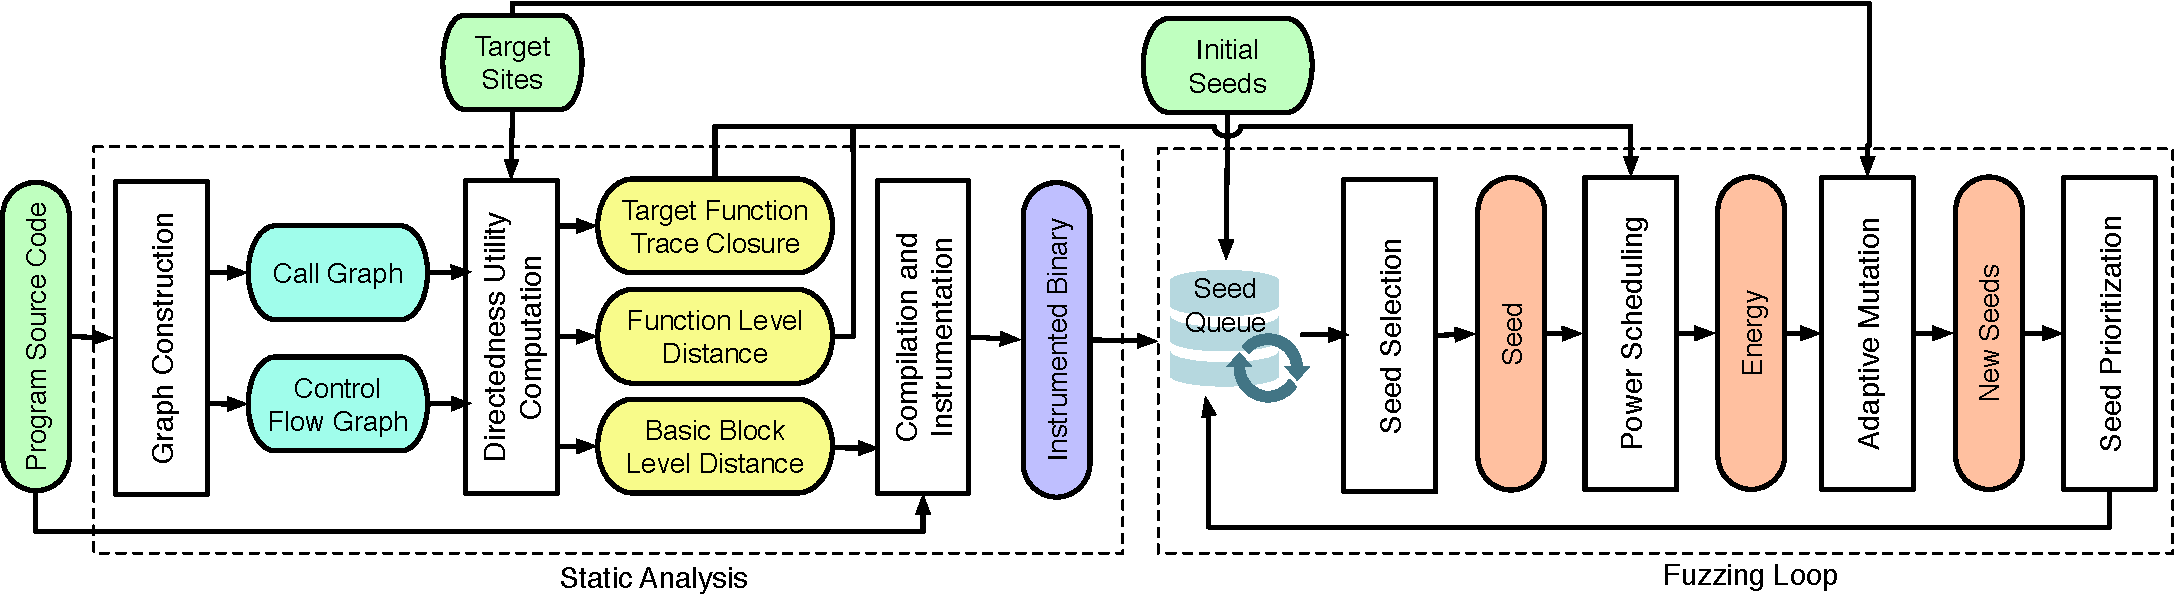
\includegraphics[width=.99\columnwidth]{res/dfot/overview.pdf}
	\caption{Approach Overview of \dFOT}
	\label{fig:overview}
\end{figure*}

\textbf{For P1.} 
In \aflgo, the seed distance to a specific target basicblock/function is calculated as the average shortest distance of basicblocks/function the seed covers. For example, in Figure~\ref{fig:call_chain}, where the nodes are functions, for trace $a\rightarrow b\rightarrow c\rightarrow d\rightarrow T\rightarrow Z$, given the fact that $d(a, T)=2$ (shortest path: $a\rightarrow e\rightarrow T$), $d(b,T)=3$ (shortest path: $b\rightarrow c\rightarrow d\rightarrow T$), $d(c,T)=2$ (shortest path: $c\rightarrow d\rightarrow T$), $d(d,T)=1$ (shortest path: $d\rightarrow T$), we can see $d_s(\langle a,b,c,d,T,Z\rangle)=(2+3+2+1+0)/5=1.6$. Analogously, $d_s(\langle a,e,T,Z\rangle)=(2+1+0)/3=1$ and $d_s(\langle a,e,f,Z\rangle)=(2+1)/2=1.5$~\footnote{In practice, \aflgo calculates the trace distance at the \emph{basicblock} level with harmonic mean of the accumulative distance; nevertheless, the essential idea is the same.}. 
Given these three execution traces, the energy assigned to them will be $ \langle a, e, T, Z\rangle$ $>$ $\langle a, e, f , Z\rangle$ $>$ $\langle a, b, c, d, T, Z\rangle$.
This is problematic: the normal trace $\langle a, e, T, Z\rangle $ is overemphasized; the crashing trace $\langle a, b, c, d, T, Z\rangle$ is however considered the least important, even less important than the trace $\langle a, e, f , Z\rangle$ that fails to reach the target $T$.



\textbf{For P2.} AFLGo only considers explicit call graph.
Due to this, all function pointers are treated as \emph{external nodes} which 
are ignored during distance calculation. 
This means that, in an extreme case, if the target function is called via a function pointer, its distance from the actual caller is undefined. 
For example, in Figure~\ref{fig:call_chain}, if $d$ and $e$ call $T$ via function pointers, both $d$ and $e$ will be mistakenly considered unreachable to $T$; consequently, all nodes except for $T$ will be considered unreachable to $T$. Therefore essentially there is no directedness in such a case.
Besides, \aflgo counts the same callee in its callers only once, and does not differentiate various call patterns between the caller and callee (see \S\ref{subsec:functionDist}).
The function level distance is calculated on the call graph with the Dijkstra shortest path, assuming the weight of two adjacent nodes (functions) in the call graph always to be 1, which will distort the distance calculation. 


\textbf{For P3. } 
\aflgo applies a simulated annealing based power scheduler: it favors those seeds that are closer~to~the target locations by assigning more energy to them for mutation; the applied cooling schedule initially assigns smaller weight on the effect of ``distance guidance'', until it reaches the ``exploitation'' phrase. It solves the ``exploration vs exploitation'' problem~\cite{eve} and mitigates the imprecision issue brought by the statically calculated basicblock level distance. In our opinion, this is an effective strategy. The problem is that there lacks a prioritization procedure so the newly generated seeds with smaller distance may wait for a long to be mutated.


 
\textbf{For P4. } The mutation of \aflgo come from AFL's two non-deterministic strategies: 1) \emph{havoc}, which does purely random mutations such as bit flips, chunk replacement, etc; 2) \emph{splice}, which generates seeds from some random byte parts of two existing seeds. 
Notably, during runtime \aflgo excludes all the deterministic mutation procedures and relies purely on the power scheduling on havoc/splice strategies.
The randomness of these two strategies can indeed favor those with smaller distances to the target locations.
However, it may also destroy the existing seeds that are close to them.
In fact, some subtle vulnerabilities can only be reached with some special preconditions. In reality, an incomplete fix may still leave some concern cases to be vulnerable; for example, CVE-2017-15939 is caused by an incomplete fix for CVE-2017-15023.
Hence, \aflgo lacks the adaptive mutation strategies, which will mutate arbitrarily even when the current seeds are close to the specified locations enough.


\textbf{Summary.} We summarize the following suggestions to improve DGFs:
\begin{enumerate}[(1)] 
	\itemsep0em
	\item For \textbf{P1}, an accurate distance definition is needed to retain trace diversity and mitigate the bias on short traces.
	\item For \textbf{P2}, both direct and indirect calls need to be analyzed; different call patterns need to be distinguished during static distance calculation.
	\item For \textbf{P3}, a moderation to the current power scheduling and a distance-guided seed prioritization strategy are preferable.
	\item For \textbf{P4}, an adaptive mutation strategy is needed to optimally apply fine-grained and coarse-grained mutations.
\end{enumerate}


\section{Approach Overview}

In this section, we briefly introduce the workflow of our proposed approach, named \dFOT. An overview of \dFOT is given in Figure~\ref{fig:overview}, which~consists of two major components, i.e., \textit{static analysis} and \textit{fuzzing loop}. 



\subsection{Static Analysis}\label{subsec:static_flow}

The inputs of static analysis are the \textit{program source code} and the~\textit{target locations} (i.e., the lines of code that the fuzzer is directed to reach). We derive the basicblocks and functions where the target locations reside in, and call them \textit{target basicblocks} and \textit{target functions}, respectively. The main output of static analysis is the \textit{instrumented program~binary} with the information of \textit{basicblock level distance}.

Firstly, we precisely construct the call graph (CG) of the target~program based on the inclusion-based pointer analysis~\cite{Andersen94programanalysis} to include all the possible calls. For each function, we construct its  control flow graph (CFG) (\S\ref{subsec:graghCons}).

Secondly, we compute several~utilities to facilitate the directedness in \dFOT based on CG and CFG (\S\ref{subsec:UtilityComputation}).
\begin{enumerate}[(1)]
\item \textbf{Function level distance} is computed based on CG by augmenting adjacent-function distance (\S\ref{subsec:functionDist}).~This distance is utilized~to calculate the \textit{basicblock level distance}. It is also~used during the fuzzing loop to calculate the \emph{covered function similarity} (\S\ref{subsec:powerSche}).
    
\item \textbf{Basic block level distance} is computed based on the function level distance with the CG and the functions' CFGs. This distance is statically instrumented for each basicblock considered to be able to reach one of the target locations. In the fuzzing loop, it is also used to calculate the \emph{basicblock trace distance} (\S\ref{subsec:powerSche}).

\item \textbf{Target function trace closure} is computed for each target location~according to the CG to obtain the functions that can reach the target locations. It is used during the fuzzing loop to calculate the \emph{covered function similarity} (\S\ref{subsec:powerSche}).
\end{enumerate}

Lastly, the target program is instrumented to keep track of the edge transitions (similar to AFL), the accumulated basicblock trace distance, and the covered functions.


\subsection{Dynamic Fuzzing Loop}\label{sec:fuzz_flow}

The inputs of fuzzing loop are the \textit{instrumented program binary},~the \textit{initial seeds}, the \textit{target locations} as well as the information of \textit{function level distance} and \textit{target function trace closure}.
The outputs~of~fuzzing loop are the seeds that cause abnormal program behaviors such as crashes or timeouts.

During fuzzing, the fuzzer selects a seed from a priority seed queue. The fuzzer applies a \textit{power scheduling} against the seed with~the goal of giving those seeds that are considered to be ``closer'' to the target locations more mutation chances (a.k.a. energy, \S\ref{subsec:powerSche}). Specifically, this is achieved through a power function, which is a combination of the \textit{covered function similarity} and the \textit{basicblock trace distance}. For each newly generated seed during mutation, after capturing its execution trace, the fuzzer will calculate the covered function similarity and the basicblock trace distance based on the utilities (\S\ref{subsec:static_flow}). For each input execution trace, its basicblock trace distance is calculated as the accumulated basicblock level distances divided by the total number of executed basicblocks; and its covered function similarity is calculated based on the intersection of covered functions and the target function trace closure, as well as the function level distance.

After the energy is determined, the fuzzer adaptively allocates mutation budgets on two categories of mutations according to mutators' granularities on the seed (\S\ref{subsec:mutationStr}).
Afterwards, the fuzzer evaluates the newly generated seeds to prioritize those that have more energy or that have reached the target functions (\S\ref{subsec:prioritization}).



\section{Methodology}

This section elaborates the key components in Figure~\ref{fig:overview} featuring the four properties.


\subsection{Graph Construction} \label{subsec:graghCons}

To calculate the accurate distance from a seed to the target locations, we first build up the CG and CFG, then combine them to construct the final inter-procedural CFG. Note that CG is used to compute the function level distance in \S\ref{subsec:functionDist} and \S\ref{subsec:UtilityComputation}, CFG together with CG (i.e., inter-procedural CFG) is used to compute the basicblock distance in \S\ref{subsec:UtilityComputation}.




To identify the indirect call in call graph, we propose to apply the inclusion-based pointer analysis~\cite{Andersen94programanalysis} against the function pointers of the whole program. The core idea of this algorithm is to translate the input program with statements of the form \emph{p := q} to constraints of the form ``\emph{q}'s points-to set is a subset of \emph{p}'s points-to set''. 
Essentially, the propagation of the points-to set is applied with four rules namely \emph{address-of}, \emph{copy}, \emph{assign}, \emph{dereference}. This analysis is context-insensitive and flow-insensitive, meaning that it ignores both the calling context of the analyzed functions and the statement ordering inside functions, and eventually only computes a single points-to solution that holds for all the program points. Usually, a fixed point of the points-to sets will be reached at the end of the analysis. Among these, points-to sets of the function pointers inside the whole program are calculated, resulting in a relatively precise call graph including all the possible direct and indirect calls. The complexity of this pointer analysis is $\Theta(n^3)$.
The reason that we do not apply context-sensitive or flow-sensitive analyses lies in the fact that they are computationally costly and not scalable to large projects. Despite that, our call graph is still much more precise than the one generated by LLVM's builtin APIs, which does not contain any explicit nodes that represent indirect calls. 

The control flow graph of each function is generated based on LLVM's IR. The inter-procedure flow graph is constructed by collecting the call sites in all the CFGs and the CG of the whole program.  By applying these static analyses, we achieve \textbf{P2}.




\subsection{Adjacent Function Distance Augmentation} \label{subsec:functionDist}
To achieve \textbf{P1}, we propose to implement a lightweight static analysis that considers the patterns of the (immediate) call relation based on the generated call graph.
As discussed in \textbf{P2}, under different context, the distances from the calling function to the immediately called function may not be exactly the same. 
Given functions $f_a$, $f_b$, $f_c$, there may exist several different call patterns in the call graph. 
For example, in Figure~\ref{subfig:dist1} and Figure~\ref{subfig:dist2}, there are calls $f_a\rightarrow f_b$  and  $f_a\rightarrow f_c$ in both cases. 
However, in Figure~\ref{subfig:dist1}  $f_a$ is bound to call $f_b$ (since $f_b$ appears in both \emph{if} and \emph{else} branches in $f_a$), but not necessary to call $f_c$; in Figure~\ref{subfig:dist2}, both $f_b$ and $f_c$ are not necessary to be called by $f_a$.
From a probability perspective, we would think that in both cases the distance from $f_a$ to $f_b$ should be smaller than the distance from $f_a$ to $f_c$, and the distance from $f_a$ to $f_b$ in Figure~\ref{subfig:dist1} should be smaller than that in  Figure~\ref{subfig:dist2}. 


\begin{figure}[t]
    \centering
\begin{subfigure}[b]{0.36\columnwidth}
\begin{lstlisting}[language=c]
void fa(int i) {
  if (i > 0) {
    fb(i);
  } else {
    fb(i*2);
    fc();
  }
}
\end{lstlisting}  
\caption{}
\label{subfig:dist1}      
\end{subfigure}
\hspace{0.1in}
\centering
\begin{subfigure}[b]{0.36\columnwidth}
\begin{lstlisting}[language=c]        
void fa(int i) {
  if (i > 0) {
    fb(i);
    fb(i*2);
  } else {
    fc();
  }
}        
\end{lstlisting}
\caption{}
\label{subfig:dist2}      
\end{subfigure}
\caption{An example that illustrates different call patterns.}
\label{figure:dists}
\end{figure}

Therefore, we propose two metrics to augment the distance that is defined by immediate calling relation between caller and callee.
\begin{enumerate}[(1)] 
\item Call site occurrences $\csnumn{f_1}{f_2}$~of a certain callee $f_2$ for a given caller $f_1$. More occurrences of callee could incur more chance that callee will be dynamically executed with more different (actual) parameters, and in return the distance between the caller to the callee will be smaller. We apply a factor $\Phi(f_1,f_2)=\frac{\phi\cdot \csnumn{f_1}{f_2}+1}{\phi\cdot \csnumn{f_1}{f_2}}$ to denote this effect, where $\phi$ is a constant value.
\item The number of basicblocks $\csbbn{f_1}{f_2}$~in the caller that contains at least one call site of the callee. The rationale is that, with more branches that have a call site, more different execution traces will include the callee. The factor function $\Psi(f_1,f_2)=\frac{\psi\cdot \csbbn{f_1}{f_2}+1}{\psi\cdot \csbbn{f_1}{f_2}}$ denotes this effect, and $\psi$ is a constant value.
\end{enumerate}

By default, we choose $\phi=2$ and $\psi=2$, to balance the effects of the considered two metrics.
Note that both factor functions are monotone decreasing functions; also, $\Phi(f_1,f_2)$ converges to 1 when $\csnumn{f_1}{f_2}\rightarrow\infty$ and $\Psi(f_1,f_2)$ converges to 1 when $\csbbn{f_1}{f_2}\rightarrow 1$.
Given a (direct or indirect) immediate function call pair $( f_1, f_2)$ where $f_1$ is the caller and $f_2$ is the callee, the original distance between $f_1$ and $f_2$ is 1. Now, with the two metrics mentioned above, we can define the augmented distance between the function pairs that holds an immediate call relation. The final adjustment factor will be a multiplication of $\Phi$ and $\Psi$, and the \emph{augmented adjacent-function distance} is
{\myeqsize\begin{equation}
 \traceFnDistPrime{f_1}{f_2} =  \Psi(f_1, f_2)\cdot\Phi(f_1, f_2)
\end{equation}}
where $\traceFnDistPrime{f_1}{f_2}$ refers to the \emph{augmented} \emph{direct} function distance. 

 As an example, in Figure~\ref{subfig:dist1}, for $f_b$, $\csnumn{f_a}{f_b}=2$, $\csbbn{f_a}{f_b}=2$; and for $f_c$, $\csnumn{f_a}{f_c}=1$, $\csbbn{f_a}{f_c}=1$. Assume $\phi=2$ and $\psi=2$ and assume the original distance $\traceFnDist{f_a}{f_b}=\traceFnDist{f_a}{f_c}=1$, the augmented distances will be $\traceFnDistPrime{f_a}{f_c}=\frac{3}{2}\cdot\frac{3}{2}=2.25$, and $\traceFnDistPrime{f_a}{f_b}=\frac{5}{4}\cdot\frac{5}{4}=1.56$.


A special case not shown in the above examples is that some branches form cycles (i.e., loops). Indeed, these functions may be called multiple times at runtime. However, it is uncertain the sense that \emph{how many times} they will be executed across different runs when fed with different seeds. Fortunately, actual execution on one call site of a callee inside one loop typically has similar effect --- the loop explores the similar program states and benefits less in covering new paths. Hence, the function call inside the loop does not bring many execution trace diversities like the scenario where the same callee occurs in multiples branches with significantly different parameters. In the future, we plan to apply loop summarizations based on invariants~\cite{issta15-slooper,loopinv,loopster,xie2016proteus,xie2017automatic,fib} to specialize these cases.

The applied approach aims to make a trade-off between the efficiency and the utility of the static analysis. Therefore, we do not consider the solution space of any branch condition that may affect the \emph{runtime reachability} in the CFG. For example, in Figure~\ref{subfig:dist1}, if we change the condition check ${i>0}$ to be ${i==0}$, the true branch will be executed only when the input value of $i$ is 0. It is tempting to assign a smaller distance to the code segments in the false branch. However, since the target program is usually nontrivial, it is impractical to statically formulate the exact constraint set of the preconditions before reaching function $f_a$ and predicate the branches's actual execution probabilities. One common scenario is that the branch condition \emph{i==0} is used for checking the return status code of an external function call, at runtime it may actually execute the true branch more often than the false branch.




\subsection{Directedness Utility Computation} \label{subsec:UtilityComputation}

In \S\ref{subsec:functionDist}, the augmented function distance is calculated on two adjacent functions according to their call patterns. By assigning  the adjacent-function distance as the weight of the edges in the call graph, we can calculate the function level distance for any two functions with the Dijkstra shortest path algorithm, beyond which we can further derive the 
basicblock level distance. 
Besides, we also compute the target function trace closure which will be used to calculate the covered function similarity in \S\ref{subsec:powerSche}.

\textbf{Function Level Distance.} This distance is calculated according to CG. It tells the (average) distance from the current function to target functions. Given a function $n$, its distance to the target function set \tgtfnset~is defined as:
{\myeqsize\begin{equation}
d_f(n, \tgtfnset) =
\begin{cases}
\textbf{undefined.} & \text{if}~R(n, \tgtfnset)=\emptyset \\
[\Sigma_{\tgtfn\in R(n, \tgtfnset)} \traceFnDist{n}{\tgtfn}^{-1}]^{-1} & \textmd{otherwise} \\
\end{cases}
\label{eq:aflgo_func_dist}
\end{equation}}
where $R(n, \tgtfnset) = \left\{\tgtfn | \textbf{reachable}(n, \tgtfn)\right\}$,
which is the set of target functions that can be statically reached from $n$ in CG, and \traceFnDist{n}{\tgtfn} is the \emph{dijkstra shortest path based on augmented function distance} from $n$ to a given target function {\tgtfn} in CG.

\textbf{Basic Block Level Distance.} Given a function $n$ and two basicblocks $m_1$ and $m_2$ inside, the basicblock level distance \simpleBBDist{m_1}{m_2} is defined as the minimal number of edges from $m_1$ to $m_2$ in the CFG \cfg{n}.
The set of functions called inside basicblock $m$ is denoted as \BBCallees{m},
then $\BBCalleesT{m}=\left\{n | R(n, \tgtfnset)\neq\emptyset, n\in\BBCallees{m} \right\}$, 
and $\transitiveBB=\left\{m| \exists \cfg{n}, m\in \cfg{n}, n\in\fnset, \BBCalleesT{m}\neq\emptyset \right\}$, where $\fnset$ is the set of all functions.
Given a basicblock $m$, its distance to the target basicblocks \tgtbbset~are defined as:
{\myeqsize\begin{equation}
\traceBBDist{m}{\tgtbbset} = 
\begin{cases}
0 & \textbf{if}~m\in \tgtbbset \\
c\cdot \text{min}_{n\in \BBCalleesT{m}}(\traceFnDist{n}{\tgtfnset})& \textbf{if}~m\in \transitiveBB\\
\Large[\Sigma_{t\in\transitiveBB}\large(\simpleBBDist{m}{t} + \traceBBDist{t}{\tgtbbset}\large)^{-1}\Large]^{-1} & otherwise
\end{cases}
\label{eq:aflgo_bb_dist}
\end{equation}}
where $c$ is a constant that magnifies function level distance.

Note that Equation \ref{eq:aflgo_func_dist} and \ref{eq:aflgo_bb_dist}, on their own, are the same as those in \aflgo \cite{Bohme:2017:DGF}. However, $\traceFnDist{n}{\tgtfn}$ for these equations in \aflgo is simply the Dijkstra shortest distance on a CG where the weight of edges (i.e., adjacent function distance) is 1.

\textbf{Target Function Trace Closure.} This utility, $\fntrace{\tgtfnset}$,  is calculated by collecting all the predecessors that can statically lead to the target functions $\tgtfnset$, until the entry function \emph{main} has been reached. We choose \emph{not} to exclude those that are \emph{considered} unreachable from entry function due to the limitations of static analysis. In the example in Figure~\ref{fig:call_chain}, $\xi_f(T_f)=\{a,b,c,d,e,T\}$.




\subsection{Power Scheduling}  \label{subsec:powerSche}

During fuzzing, we apply power scheduling on a selected seed based on two dynamically computed metrics: basicblock trace distance and target function trace similarity.

\textbf{Basic Block Trace Distance.} The distance between seed $s$ to the target basicblocks $\tgtbbset$ is defined as:
{\myeqsize\begin{equation}
\traceDist{s}{\tgtbbset} = \frac{\Sigma_{m\in\xi_b(s)}\traceBBDist{m}{\tgtbbset}}{|\bbtrace{s}|}
\label{eq:aflgo_seed_dist}
\end{equation}}
where \bbtrace{s} is the execution trace of a seed $s$ and contains all the basicblocks that are executed. Hence, the basic idea of Equation  \ref{eq:aflgo_seed_dist} is that: for all the basicblocks in the  execution trace of $s$, we calculate the average basicblock level distance to the target basicblocks  $\tgtbbset$.  Note that Equation \ref{eq:aflgo_seed_dist} is also the same as the one in \aflgo \cite{Bohme:2017:DGF}.

It then applies a feature scaling normalization to get the final distance $\traceDistFinal{s}{\tgtbbset}=\frac{\traceDist{s}{\tgtbbset}-minD}{maxD-minD}$ where $minD$ (or $maxD$) is the smallest (or largest) distances ever met.


\textbf{Covered Function Similarity.} This metric measures the similarity between a seed's execution trace and the target execution trace \emph{at function level}. We do not track basicblock level trace similarity since that would introduce considerable overheads. The similarity is calculated based on the intuition that seeds covering more functions in the expected traces have more chances to be mutated to reach the target locations. This similarity is calculated by tracking the seed's covered function \emph{sets} (denoted as \fntrace{s}) and comparing it with the target function trace closure $\fntrace{\tgtfnset}$.  In the example in Figure~\ref{fig:call_chain}, $\xi_f(\langle a,b,c,d,T,Z\rangle)=\{a,b,c,d,T\}$, $\xi_f(\langle a,e,T,Z\rangle)=\{a,e,T\}$ and $\xi_f(aefZ)=\{a,e\}$.

The covered function similarity is then determined by the following formula:
{\myeqsize\begin{equation}
\covDist{s}{\tgtfnset} = \frac{\Sigma_{f\in\fntrace{s}	\cap\fntrace{\tgtfnset}}\traceFnDist{f}{\tgtfnset}^{-1}}{|\fntrace{s}\cup\fntrace{\tgtfnset}|}
\end{equation}}
$\traceFnDist{f}{\tgtfnset}$ is the function level distance calculated with Equation~\ref{eq:aflgo_func_dist}. Similar to \traceDistn, a feature scaling normalization is also applied and the final similarity is denoted as \covDistnN. Note that this similarity metric is uniquely proposed in our approach.

\textbf{Scheduling.}
Scheduling deals with the problem how many mutation chances will be assigned to the given seed. The intuition is that if the trace that the current seed executes is ``closer'' to any of the expected traces that can reach the target location in the program, more mutations on that seed should be more beneficial for generating expected seeds. A scheduling purely based on \emph{trace distance} may favor certain patterns of traces. For \aflgo, as mentioned in \textbf{P2}, the shorter paths will be assigned more energy, which may starve longer paths that are still reachable to the target locations. To \emph{mitigate} this, we propose the \emph{power function} that considers both \emph{trace distance} (based on basicblock level distance) and \emph{trace similarities} (based on covered function similarity): 
{\myeqsize\begin{equation}\label{eq:aflgo_power}
p(s, \tgtbbset) = \covDistN{s}{\tgtfnset}\cdot(1 - \traceDistFinal{s}{\tgtbbset})
\end{equation}}
Obviously, the value of $p(s, \tgtbbset)$ fits into $[0,1]$ since both the multipliers are in $[0,1]$.

Compared to AFLGo's approach, which only considers basicblock trace distance (\traceDistn, or \traceDistnFinal), our power function balances the effect of shorter paths and the longer paths that can reach the target. Logically, there are some differences between {\covDistn} and {\traceDistn}:
\begin{enumerate}[(1)]
    \item \traceDistn~considers both the effects of CG and the CFGs; {\covDistn} considers only the effects of CG. For \traceDistn, the major effect is still CG due to the magnification factor $c$ used in Equation~\ref{eq:aflgo_func_dist}.
    \item \traceDistn~does not penalize traces that do not lead to the target locations, while {\covDistn} penalizes them via a union of \fntrace{s} (by tracking function level traces) and \fntrace{\tgtfnset}.
    \item Given multiple traces that can lead to the target locations, {\traceDistn} favors those that have shorter lengths, but {\covDistn} favors those with longer lengths of common functions in expected trace.
\end{enumerate}

In this sense, $p(s, \tgtbbset)$ strives a balance between shorter traces and longer traces that can reach the target locations with \emph{two heterogeneous metrics}. Admittedly, there may still exist some bias. One of the scenarios is that the power function may assign more energy to a seed that covers many functions in the target function trace closure. For example, assume two traces that can reach the target function $T$: $\langle a,b,c,d,T,Z\rangle$ and $\langle a,e,f,g,T,Z\rangle$; and the target function trace closure is $\langle a, b, c,d,e,f,g,T\rangle$. The power function may assign much energy to a seed with trace $\langle a, b, c, d, e, f, g, Z\rangle$ which does not reach the target function $T$. This is \emph{not} an issue in our opinion: since this seed has covered many ``expected'' functions, it has high chance to be ``close'' to the target; with proper mutations, it is likely to be flipped to mutants that can indeed touch the target.

In {\dFOT}, the power function determines the number of mutation chances to be applied on the current seed (i.e., energy); it is also used during the seed prioritization to determine whether the \emph{mutated} seeds should be favored.

\subsection{Adaptive Mutation} \label{subsec:mutationStr}

\begin{algorithm}[t]
	\setstretch{0.9}
	\small	
	\SetKwInOut{Input}{input}\SetKwInOut{Output}{output}
	\SetKwInOut{Const}{const.}
	\Input{$s$, the seed to be fuzzed  after power scheduling}
	\Output{$\mathcal{M}_s$, the map to store the new mutated seed, whose key is the seed and whole value is the energy of the seed}
	\Const{$\gamma$, the constant ratio to do fine-grained mutation}
	\Const{$\delta$, the constant ratio to be adjusted}
	\BlankLine
	\SetKw{Continue}{\textbf{continue}}
	\SetKw{And}{\textbf{and}}
	\SetKw{Not}{\textbf{not}}
	\SetKw{Is}{\textbf{is}}
	\SetKw{In}{\textbf{in}}
	\SetKw{Or}{\textbf{or}}
	\SetKw{Eqs}{\textbf{equals}}
	\SetKw{Fori}{\textbf{for}}
	\SetKwProg{Def}{def}{:}{}
$\mathcal{M}_s = \emptyset$\;
	 $p\leftarrow s.getScore()$\; \label{algo1:getscore}
	\If{$ reachTarget(s) == false$}{ \label{algo1:ifcheck}
$\mathcal{S}^{\prime} \leftarrow  coarseMutate(s, p *(1- 	\gamma ))$\; \label{algo1:old_coarse}
	    \For{$s^{\prime}$ in $\mathcal{S}^{\prime}$}{
$\mathcal{M}_s\leftarrow \mathcal{M}_s \cup  \{(s^{\prime},s^{\prime}.getScore())\} $
	    }
   		$\mathcal{S}^{\prime\prime} \leftarrow  fineMutate(s, p * 	\gamma )$\; \label{algo1:old_fine}
    	\For{$s^{\prime\prime}$ in $\mathcal{S}^{\prime\prime}$}{
$\mathcal{M}_s\leftarrow \mathcal{M}_s \cup  \{(s^{\prime\prime},s^{\prime\prime}.getScore())\} $
  		}
	 }
     \Else{ \label{algo1:elsecheck}
     	   
     $\mathcal{S}^{\prime} \leftarrow  coarseMutate(s, p *(1- 	\gamma -\delta ))$\;\label{algo1:new_coarse}
     \For{$s^{\prime}$ in $\mathcal{S}^{\prime}$}{
$\mathcal{M}_s\leftarrow \mathcal{M}_s \cup  \{(s^{\prime},s^{\prime}.getScore())\} $
     }
     $\mathcal{S}^{\prime\prime} \leftarrow  fineMutate(s, p *(	\gamma + \delta))$\; \label{algo1:new_fine}
     \For{$s^{\prime\prime}$ in $\mathcal{S}^{\prime\prime}$}{
$\mathcal{M}_s\leftarrow \mathcal{M}_s \cup  \{(s^{\prime\prime},s^{\prime\prime}.getScore() )\} $
     }
 	}
 
  
	\caption{$adaptiveMutate()$: Adaptive Mutation}
	\label{algo:mutateStr}
\end{algorithm}

In \S\ref{subsec:powerSche}, for each seed, the output of power scheduling is the energy (a.k.a. the times of applied mutations), which will be the input of the step of our adaptive mutation. The problem is that, given the total energy available for a seed, we still need to assign the number of mutations for \emph{each type of mutators}. 


In general, two categories of mutators are used in GBFs. Some are coarse-grained in the sense that they change a bulk of bytes during the mutations. Others are fine-grained since they only involve a few byte-level modifications, insertions or deletions. For coarse-grained mutations, we consider them to be:
\begin{enumerate}[(1)] 
	\item \textbf{Mixed havoc}. It includes several chunk mutations, namely deleting a bulk of bytes, overwriting the given chunk with other bytes in the buffer, deleting a certain lines, duplicating certain lines multiple times, etc. The actual mutation involves their combinations.
	\item \textbf{Semantic mutation}. It is used when the target program is known to process semantic relevant input files such as javascript, xml, css, etc. In detail, this follows Skyfire~\cite{junjie:2017sp:skyfire}, which includes three meta mutations, inserting another subtree into a random AST position, deleting a given AST, and replacing the given position with another AST.
	\item \textbf{Splice}. It includes a crossover between two seeds in the queue and subsequent mixed havocs.
\end{enumerate}


Algorithm~\ref{algo:mutateStr} shows the workflow of our adaptive mutation, given a seed $s$. 
The basic idea is to give less chance of coarse-grained mutations when the seed $s$ can reach the target functions (at line \ref{algo1:elsecheck} in Algorithm~\ref{algo:mutateStr}). Once the seed reaches the target locations, the times of doing fine-grained mutations increase from  $ p * 	\gamma$ (line \ref{algo1:old_fine}) to $p *(	\gamma + \delta)$ (line \ref{algo1:new_fine}), but the times of doing coarse-grained mutation decrease from  $ p *(1- 	\gamma )$ (at line \ref{algo1:old_coarse}) to $p *(1- 	\gamma -\delta )$ (line \ref{algo1:new_coarse}). Here, $s.getScore()$ at line \ref{algo1:getscore} is to get the energy assigned to the seed according to the the power function value calculated in Equation~\ref{eq:aflgo_power}.

\begin{algorithm}[t]
	\setstretch{0.9}
	\small	
	\SetKwInOut{Input}{input}\SetKwInOut{Output}{output}
	\SetKwInOut{Const}{const.}
	\Input{$s$, the seed to be fuzzed  after power scheduling}
	\Input{$i$, the number of iterations to do mutation on the seed}
	\Output{$\mathcal{S}$, the set to store the \emph{new} mutated seed}
	\Const{$\sigma$, the constant ratio to do semantic mutations}
	\Const{$\zeta$, the constant ratio to do mixed havoc mutations}
	\BlankLine
	\SetKw{Continue}{\textbf{continue}}
	\SetKw{And}{\textbf{and}}
	\SetKw{Not}{\textbf{not}}
	\SetKw{Is}{\textbf{is}}
	\SetKw{In}{\textbf{in}}
	\SetKw{Or}{\textbf{or}}
	\SetKw{Eqs}{\textbf{equals}}
	\SetKw{Fori}{\textbf{for}}
	\SetKwProg{Def}{def}{:}{}
	
	$\mathcal{S} = \emptyset$\;	
 	\If{$needSemMutation(s) == true $}{ \label{algo2:checkSem}
 		$\mathcal{S} \leftarrow \mathcal{S} \cup semMutate(s, i * \sigma)$	\;	\label{algo2:applySem}
 		$\mathcal{S} \leftarrow \mathcal{S} \cup coarseHavoc(s, i * (1-\sigma) * \zeta)$\;		\label{algo2:applyHavoc1}
 			$\mathcal{S} \leftarrow \mathcal{S} \cup splice(s, i * (1-\sigma) * (1-\zeta))$	\;	\label{algo2:applysplice1}
}
    \Else{  \label{algo2:checkSemElse}
       	$\mathcal{S} \leftarrow \mathcal{S} \cup coarseHavoc(s, i * \zeta)$\;		\label{algo2:applyHavoc2}
        $\mathcal{S} \leftarrow \mathcal{S} \cup splice(s, i * (1-\zeta))$	\;		\label{algo2:applysplice2}
    }
	\caption{$coarseMutate()$: Coarse-Grained Mutation}
	\label{algo:coarseMutate}
\end{algorithm}
 
$fineMutate()$ in  Algorithm~\ref{algo:mutateStr}  simply  applies a random fine-grained mutation (e.g., bit/byte flippings, arithmetics  on some bytes) for the seed. Algorithm~\ref{algo:coarseMutate} shows the details for coarse-grained mutation strategy  $coarseMutate()$. Given a seed $s$ and the iteration times of mutations $i$, the basic idea is to apply semantic mutations (line \ref{algo2:checkSem}) only  when it is  necessary (line \ref{algo2:applySem}). The constraints $needSemMutation(s)$ returns true if the following conditions are satisfied: 1) our fuzzer detects that the input file is  a semantic-relevant input file such as javascript, xml, css, etc; 2) The previous semantic mutations have not failed. Otherwise (line \ref{algo2:checkSemElse}), mixed havoc mutations will get more times ($i * \zeta$, at line \ref{algo2:applyHavoc2}) than the necessary case ($i * (1-\sigma) * \zeta$, at line \ref{algo2:applyHavoc1}), meanwhile splice mutations will also get more times ($ i * (1-\zeta)$ line \ref{algo2:applysplice2}) than necessary ($i * (1-\sigma) * (1-\zeta)$, at line \ref{algo2:applysplice1}).
In practice, we assign empirical values to: $\gamma=0.1$, $\delta=0.4$, $\sigma=0.2$, $\zeta=0.8$.



Note that all these new generated  seeds in $\mathcal{M}_s $, together with the original seeds, will be put into the seed queue for future fuzzing. Actually, before fuzzing them, we will prioritize them to improve the efficiency of directed fuzzing (see \S\ref{subsec:prioritization}).




\begin{algorithm}[t]
	\setstretch{0.9}
	\small	
	\SetKwInOut{Input}{input}\SetKwInOut{Output}{output}
	\SetKwInOut{Const}{const.}
	\Input{$s$, the seed to be processed}
	\Output{$\mathcal{Q}_1$, the tier 1 queue to store the most important seeds}
	\Output{$\mathcal{Q}_2$, the tier 2 queue to store the important  seeds}
	\Output{$\mathcal{Q}_3$, the tier 3 queue to store the least important seeds}
	\Const{$\mu$, the threshold of energy value for accepting important seeds}
	\BlankLine
	\SetKw{Continue}{\textbf{continue}}
	\SetKw{And}{\textbf{and}}
	\SetKw{Not}{\textbf{not}}
	\SetKw{Is}{\textbf{is}}
	\SetKw{In}{\textbf{in}}
	\SetKw{Or}{\textbf{or}}
	\SetKw{Eqs}{\textbf{equals}}
	\SetKw{Fori}{\textbf{for}}
	\SetKwProg{Def}{def}{:}{}
	
	$\mathcal{Q}_1 = \mathcal{Q}_2 = \mathcal{Q}_3 = \emptyset$\;	
 	\If{$seedIsNew(s) == true $}{ \label{algo3:checkNew}
  			\If{$seedWithNewEdge(s) == true $}{ \label{algo3:checkNewEdge}
  				$\mathcal{Q}_1 \leftarrow \mathcal{Q}_1 \cup \{s\} $\;	
  			}
  			\ElseIf{$s.powerEnergy() > \mu $}{ \label{algo3:bigEnergy}
  			$\mathcal{Q}_1 \leftarrow \mathcal{Q}_1 \cup \{s\} $\;	
  			}
  			\ElseIf{$reachTarget(s) == true $}{ \label{algo3:reachTarget}
  			$\mathcal{Q}_1 \leftarrow \mathcal{Q}_1 \cup \{s\} $\;	
  			}
  		    \Else{  \label{algo3:checkElse2}
  		    	$\mathcal{Q}_2 \leftarrow \mathcal{Q}_2 \cup \{s\} $\;		 	    	
  		    }
 	}
    \Else{  \label{algo3:checkNewElse}
       	$\mathcal{Q}_3 \leftarrow \mathcal{Q}_3 \cup \{s\} $\;		 
     
    }
	\caption{Seed Prioritization}
	\label{algo:seedprioritization}
\end{algorithm}
 


\subsection{Seed Prioritization} \label{subsec:prioritization}

 Not all the seeds have equal or similar priorities, ideally the queue that stores the seeds to be mutated should be a priority queue. However the scoring may be biased (due to the limitations of static analyses, etc.), and the insertion operations on priority queue take a complexity of $\Theta(\log n)$, which is costly since the queue can be quite long and the insertion operation can be frequent. Therefore it is not beneficial \emph{in practice}~\footnote{In fact, the well-known AFL fuzzer only maintains a linked list with some probabilistic to skip seeds that do not cover new edges; the complexity of the  insertion  is $\Theta(1)$.}. Instead, we provide a three-tiered queue which appends newly generated seeds into different categories according to their scores. Seeds in the top-tiered queue (tier 1) will be picked firstly, then the second-tiered (tier 2), and finally the lower-tiered (tier 3). This imitates a simplified priority queue with constant time complexity.
 
 
 Algorithm~\ref{algo:seedprioritization} shows the seed prioritization strategy for a new seed mutated from the previous step of adaptive mutation. The basic idea is: we should prioritize the \emph{newly generated} seeds that 1) cover new traces 2) have bigger similarity values with the target seeds (i.e., power function values) 3) cover the target functions. We favor seeds that cover new traces since we still have to explore \emph{more execution paths} that have the potential to lead to the target locations; this is necessary when the initial seeds are far from the target locations. The other two prioritization strategies, i.e., comparing similarity values and checking whether the target function have been reached, are specific to directed fuzzing. Note that although these two strategies are relevant, neither of them can be deduced from the other. For the other newly generated seeds, they are put in the second-tiered queue. On the other hand, seeds that have (just) been mutated are assigned with the least priority.
In practice, \dFOT also applies AFL's loop bucket approach (see ~\cite{afl_detail}) to filter out a large number of ``equivalent'' seeds that bring no new coverage as to loop iterations. The prioritization strategies will be applied on the remaining seeds. Therefore, there will not be too many seeds filling up the top-tier queue.

By combining all the static and dynamic techniques mentioned above, for the CVE exampled in \S\ref{subsec:motiv}, \dFOT successfully reproduced the crash with a time budget of 24 hours in 3 out of the 10 runs we conducted when fed with the same initial seeds, which is a significantly improvement on both AFL and AFLGo for this case.
 



\section{Evaluation}\label{sec:eval}

We implemented our instrumentation on top of FOT's static instrumentation mode (c.f. \S\ref{ch:fot}) and the pointer analysis is based on the interprocedural static value-flow analysis tool called SVF~\cite{Sui:2016:SVF}; this part takes about 2000 lines of C/C++ code based on the LLVM~\cite{Lattner:2004:LCF:977395.977673} infrastructure. For directed fuzzing purpose, we add another 4000 lines of code for tracing functions, calculating power function for seeds, distinguishing graininess of mutators, and so on. More details are available on \url{https://sites.google.com/view/ccs2018-fuzz}.

For each program with the given target locations, the instrumentation of {\dFOT} consists of three parts: 1) basicblock IDs that track the execution traces 2) basicblock distance information that determines basicblock trace distance and 3) function IDs that track functions that have been covered. 




\begin{table*}[t]
	\centering
	\caption{Program statistics for our tested programs.}
	\label{tbl:stats}
	\footnotesize
	\begin{tabular}{c|c|r"r|r|r"r|r"r}
		\thickhline
		\textbf{Project} &  \textbf{Program} &  \textbf{Size} &  \textbf{ics} &  \textbf{cs} &  \textbf{ics/cs} &  \textbf{\# of $C_B$\textgreater1} &  \textbf{\# of $C_N$\textgreater1}  &  \textbf{$t_s$} \\ \hline
		Binutils  &cxxfilt  & 2.8M  & 3232  & 12117 & 26.67\% & 8813  & 8879 &  735s  \\ \hline
		Oniguruma & testcu &	1.3M & 556 & 2065 & 26.93\% & 3037 & 3101 & 5s \\ \hline
		mjs & mjs & 277K & 130 & 3277 & 3.97\% & 309 & 334 & 3s \\ \hline 
		libjpeg & libjpeg & 810K & 749 & 1827 & 41.00\% & 144 & 152 & 2s \\ \hline
		libpng & libpng & 228K &  449 & 1018 & 44.11\% & 61 & 61 & 2s \\ \hline
		freetype2 & freetype & 1.6M & 627 & 5681 & 11.30\% & 6784 & 7117 & 4s \\ \thickhline                         
	\end{tabular}
\end{table*}

\subsection{Evalution Setup}\label{subsec:evalsetup}

In the experiments, we aim to answer the following questions:
\begin{enumerate}[\textbf{RQ}1]
    \item  Is it worth applying static analysis?
    \item  What are {\dFOT}'s performance in reproducing crashes on target locations?
    \item  How effective are the dynamic strategies in {\dFOT}?
    \item  What are {\dFOT}'s performance in reaching target locations?  
\end{enumerate}

\textbf{Evaluation Dataset.}
We evaluated \dFOT with diverse real-world programs:
\begin{enumerate}[(1)] 
    \item \textbf{GNU Binutils}~\cite{binutils} is a set of binary analysis tools on Linux. 
This also serves a benchmark in other works such as~\cite{Bohme:2016:CGF, Bohme:2017:DGF, FairFuzz}.
    \item \textbf{MJS}~\cite{mjs} is a JavaScript interpreter for embedded devices.
    It is used to compare \dFOT directly with {\aflgo} due to implementation limitations of the latter.
    \item \textbf{Oniguruma}~\cite{oniguruma} is a versatile regular expression library used by multiple world famous projects such as PHP~\cite{php}.
    \item \textbf{Fuzzer Test Suite}~\cite{fuzzer-test-suite} is a set of benchmarks for fuzzing engines.
    It contains several representative real-world projects.
\end{enumerate}

\textbf{Evaluation Tools.} We compare the following three fuzzers:
\begin{enumerate}[(1)] 
\item \textbf{AFL} is the current state-of-the-art GBF. It discards all the target information for the target program and only utilizes the ``basicblock transition'' instrumentation.
\item \textbf{{\aflgo}} is the state-of-the-art DGF based on AFL.
Compared to AFL, it also instruments basicblock distance information.
\item \textbf{{\dGO}} is the fuzzer whose basicblock level distance is generated with our static analysis procedure (Figure~\ref{fig:overview}), but the dynamic fuzzing is conducted by {\aflgo}.
\end{enumerate}

Here we mainly follow \aflgo's practice to only use AFL as the baseline for coverage oriented GBFs. Other techniques do not focus on directed fuzzing, and they are either orthogonal (e.g., CollAFL~\cite{CollAFL}) or may sometimes perform worse than AFL (e.g., \aflfast, as observed by \cite{Shastry:LNCS2017:Orthrus}), or not easily comparable (e.g., libFuzzer~\cite{libfuzzer}). The detailed reason is available at our website. %; in \S\ref{sec:related}, we also provide a more detailed comparison between {\dFOT} and these techniques.

In the experiments, all AFL based fuzzers (AFL, {\aflgo} and {\dGO}) are run in their ``fidgety'' mode~\cite{FidgetyAFL}. For both {\aflgo} and {\dGO}, ``time-to-exploitation'' is set to 45 minutes for the fuzzer. Except for the experiments against GNU Binutils (Table~\ref{tbl:cr_aflgo_binutils}) , where we follow exactly the setup in {\aflgo}~\cite{Bohme:2017:DGF} , all the other experiments are repeated 8 times, with a time budget of 4 hours. 
We use ``time-to-exposure'' (TTE) to measure the length of the
fuzzing campaign until the first seed is generated that triggers a given error (in~\S\ref{subsec:evalcrashrepro}) or reaches a target location (in~\S\ref{subsec:evalsrcloc}).
We use \emph{hitting round} to measure the number of runs in which a fuzzer triggers the error or reaches the target.
For all the experiments, if the fuzzer cannot find the target crash within the time budget in one run, TTE is set to the time budget value. 

Our experiments are conducted on an Intel(R) Xeon(R) CPU E5-2697 v3 @ 2.60GHz with 28 cores, running a 64-bit Ubuntu 16.04 LTS system; during experiments, we use 24 cores and retain 4 cores for other processes. 


\subsection{Static Analysis Statistics}\label{subsec:evalstatic}


In Table~\ref{tbl:stats}, the first three columns denote the projects, programs and the sizes in their LLVM bitcode form. \emph{ics} denotes the number of indirect call sites in the binary, which is calculated by counting those call sites without explicitly known callees; \emph{cs} is the number of call sites; \emph{ics/cs} denotes the percentage of indirect calls among all call sites. 
The next two columns denote the number where $\csnumn{f_1}{f_2}>1$ and $\csbbn{f_1}{f_2}>1$ between two adjacent functions $f_1$ and $f_2$, respectively. The last column denotes the time cost of call graph generation, which takes the majority of the time among all the directedness utility computation.



We can see from  the table that the chosen benchmarks have fair diversities in terms of different metrics.
It is also noticeable that the number of indirect function calls may contribute a large portion to the total number of function calls.
Specifically, in libpng, $44.11\%$ function calls are indirect function calls.
This clearly shows the importance of building precise call graphs.
Furthermore, the number of occurrences of $\csnumn{f_1}{f_2}>1$ and the number of occurrences of $\csbbn{f_1}{f_2}>1$ are also large, which shows the importance of taking into consideration the different patterns of call relations.




As to the overhead of the static directedness utility computation, except for \emph{cxxfilt}, which requires approximately 12.5 minutes to generates the call graph, call graphs of most other projects can be generated in seconds. For cxxfilt, the performance degradation lies in the inherent complexity of the project itself. From the program statistics in Table~\ref{tbl:stats}), it is obvious that the code base is bigger and the program structures are more complicated than the others. In fact, the bottleneck of the analysis is inside the pointer analysis implemented in SVF tool. We believe that it is worth the effort due to the fact that this procedure is done purely statically. And as long as the source code does not change, the call graph can be reused.


\subsection{Crash Exposure Capability}\label{subsec:evalcrashrepro}

The most common application of directed fuzzing is to try to expose the crash with some given suspicious locations that are supposed to be vulnerable, where the suspicious locations can be detected with the help of other static or dynamic vulnerability detection tools.
In this experiment, we directly compare {\dFOT} with other fuzzers on some known crashes to evaluate its crash exposure capability.

\subsubsection{Crash Reproduction against Binutils}

In the beginning, we intended to compare GNU Binutils directly with {\aflgo} in our experiments since it is an important benchmark in ~\cite{Bohme:2017:DGF} to demonstrate {\aflgo}'s directedness. However, we found that the actual implementation of {\aflgo} has a few issues~\cite{aflgo_issues} in generating static distances. Most importantly, it takes too long to calculate the distances. As a result, when we tried {\aflgo}'s static analysis on GNU Binutils 2.26, it failed to generate ``distance.cfg.txt'' which contains the distance information for instrumentation within 12 hours\footnote{{Besides the performance issue of \aflgo, another reason to reclaim \aflgo's results in Table \ref{tbl:cr_aflgo_binutils} is that the hardware environments are similar. The reason is supported by the similar results produced by AFL in \textbf{~\cite{Bohme:2017:DGF}} and our experiments.}}. Although {\aflgo} can still perform fuzzing without distance information instrumentation, the fuzzing process is no longer \emph{directed} without any distance input.
Therefore, we reclaimed the results in~\cite{Bohme:2017:DGF} to compare with ours for the GNU Binutils benchmark~\footnote{Since CVE-2016-4487/CVE-2016-4488 and CVE-2016-4492/CVE-2016-4493 share the same target locations, we treat them as the same; the reclaimed value for CVE-2016-4487/CVE-2016-4488 are also average values.}. We follow exactly the evaluation setup in~\cite{Bohme:2017:DGF} where each experiment is conducted for 20 times, with the time budget set as 8 hours; the initial input seed file only contains a line break (generated by \verb|echo "" > in/file|). The target locations we specified are based on their CVE descriptions and the backtraces of the crashes. We compare {\dFOT} with {\aflgo} and AFL; the results are shown in Table~\ref{tbl:cr_aflgo_binutils}. In {\aflgo}'s paper, the {\alz} metric~\cite{alz_metric} is used to show the possibility that one fuzzer is better than the other according to all the runs. It is ignored in Table~\ref{tbl:cr_aflgo_binutils} since we cannot get the result of each run in their experiments.

\begin{table}[t]
    \small
\centering
\caption{Crash reproduction in {\dFOT}, {\aflgo} and AFL against Binutils.}
\label{tbl:cr_aflgo_binutils}
     \begin{tabular}{c"c|r|r|c}
         \thickhline
    \textbf{CVE-ID}   & \textbf{Tool}  & \textbf{Runs} & \utte (s)  & \textbf{Factor} \\ \thickhline
    \multirow{3}{*}{\begin{tabular}[c]{@{}l@{}}2016-4487\\ 2016-4488\end{tabular}}& Hawkeye &   20    &   177   & -- \\ \cline{2-5} 
    & AFLGo  &  20  & 390 & 2.20\\ \cline{2-5} 
    &  AFL   &   20 & 630  &   3.56  \\ \hline
    \multirow{3}{*}{2016-4489} & Hawkeye & 20  &  206 & --  \\ \cline{2-5} 
     & AFLGo  &  20 &180&  0.87 \\ \cline{2-5} 
     & AFL   &   20  &  420  &   2.04  \\ \hline
    \multirow{3}{*}{2016-4490}  & Hawkeye & 20 & 103  &  -- \\ \cline{2-5} 
    & AFLGo  &  20 & 93   & 0.90  \\ \cline{2-5} 
    &   AFL   &  20 &  59   &  0.57  \\ \hline
    \multirow{3}{*}{2016-4491} & Hawkeye &  9  & 18733 &   --   \\ \cline{2-5} 
    &   AFLGo  &  5 & 23880    &    1.27     \\ \cline{2-5} 
    &        AFL   &       7    &            20760    &            1.11   \\ \hline
    \multirow{3}{*}{\begin{tabular}[c]{@{}l@{}}2016-4492\\ 2016-4493\end{tabular}} & Hawkeye &     20      &                    477                                 &       --      \\ \cline{2-5} 
    &   AFLGo  &     20   &  540  &                 1.21                                               \\ \cline{2-5} 
    &    AFL   &     20   &                         960                            &                  2.01                                              \\ \hline
    \multirow{3}{*}{2016-6131} & Hawkeye &       9     &                     17314                                &                      --                                          \\ \cline{2-5} 
    &   AFLGo  &                   6                                   &                      21180                               &                                1.22                                \\ \cline{2-5} 
     & AFL   &                    2                                  &            26340                                         &             1.52                                                   \\ \thickhline
    
\end{tabular}  
\end{table}

We can observe the following facts: 
1) For CVE-2016-4491 and CVE-2016-6131, \dFOT achieves the best results, with the most hitting rounds (both are 9 rounds) and the shortest {\utte} (18773s and 17314s). Compared with other tools, on average for both cases, \dFOT's improvements are significant in term of hitting rounds ($>20\%$) and {\utte} ($>20\%$).
2) For CVE-2016-4487/4488 and CVE-2016-4492/4493, all tools reproduce the crashes in 20 runs, and \dFOT achieves the best {\utte}. Specifically, on these two cases, \dFOT's improvement in terms of {\utte} is significant --- reducing at least $20\%$ than other tools.
3) For CVE-2016-4489 and CVE-2016-4490, all tools reproduce the crashes in all runs within 7 minutes since these bugs are relatively easy to find. 
Apparently, in such cases, directed fuzzers have no significant advantage --- in other words, when the crashes are shallow or easy to trigger, \dFOT's merits cannot show and fuzzing randomness matters for \utte.

To summarize, {\dFOT} has the real potential to fulfill directed fuzzing tasks where the target crashes are not easy to be detected.

\subsubsection{Crash Reproduction against MJS}

In order to \emph{directly} compare the performance between {\dFOT} and {\aflgo}, we chose a project called \emph{MJS}, which contains a single source file and the results are in Table~\ref{tbl:cr_aflgo_mjs}.
We used this project for direct comparison with \aflgo since \aflgo took too much time or failed to generate the distance information for other projects such as Oniguruma, libpng, etc. 
On \emph{MJS}, \aflgo took an average of 13 minutes to generate the basicblock distance for different target locations.
During experiments, the initial input seed files are all from the project's \emph{tests} directory. The target locations are selected from the crashes reported in the project's GitHub pages, which correspond to four categories of vulnerabilities, namely \emph{integer-overflow} (\#1, \url{https://github.com/cesanta/mjs/issues/57}), \emph{invalid-write} (\#2, \url{https://github.com/cesanta/mjs/issues/69}), \emph{heap-buffer-overflow} (\#3, \url{https://github.com/cesanta/mjs/issues/77}), and \emph{use-after-free} (\#4, \url{https://github.com/cesanta/mjs/issues/78}). We can observe the following facts : 
1) On \#1 and \#2,  \dFOT achieves the best results, with the most hitting rounds and the shortest {\utte} for both cases.  In terms of hitting rounds, {\dFOT} found \#1's bug in 5 runs and \#2's bug in 7 runs, while for the other two tools they only detected both crashes in 2 runs. Notably, this case is nontrivial and {\dFOT} reduces the {\utte} from about 3.5 hours to 0.5 hours.
2) On \#3, for which all the tools reproduce the crash in 8 rounds. Still, \dFOT has the highly significant improvement on {\utte}, using less than one fourth {\utte} of other tools.
3) On \#4, all the tools reproduce the crash in all rounds, and the {\utte} differences among them are not significant.
As to \alz, we can see that \dFOT exhibits really good results, for  example, the values in \#2 are both 0.95, which means \dFOT has 95\% confidence to perform better than both other tools.



 \begin{table}[t]
    \small
    \centering
    \caption{Crash reproduction in {\dFOT}, {\aflgo} and AFL against MJS.}
    \label{tbl:cr_aflgo_mjs}
    \begin{tabular}{c|c|c|r|c|c}
        \thickhline
        \textbf{Bug ID}                                                                                                                                  & \textbf{Tool}  & \textbf{Runs} & \utte (s) & \textbf{Factor} & \alz \\ \thickhline
        \multirow{3}{*}{\#1} & Hawkeye &       5                                               &         5469                                            &             --                                 & --                  \\ \cline{2-6} 
        &             AFLGo  &         2                                             &                              12581                       &                  2.30                             &     0.77            \\ \cline{2-6} 
        &             AFL   &        2                                              &                              13084                       &                       2.39                        &     0.77            \\ \hline
        \multirow{3}{*}{\#2}  & Hawkeye &       7                                               &                    1880                                 &             --                               & --                    \\ \cline{2-6} 
        &            AFLGo  &             2                                         &                    12753                                 &                6.78                           &          0.95           \\ \cline{2-6} 
        &        AFL   &             2                                         &                   12294                                  &               6.54                           &          0.95            \\ \hline
        \multirow{3}{*}{\#3} & Hawkeye &                           8                           &      178                                               &           --                     & --                                \\ \cline{2-6} 
        &       AFLGo  &         8                                             &                       819                              &                       4.60                      &           0.91        \\ \cline{2-6} 
        &        AFL   &            8                                          &                         1269                            &                     7.13                   &              0.95          \\ \hline
        \multirow{3}{*}{\#4}  & Hawkeye &      8                                                &                 5519                                    &              --                         & --                         \\ \cline{2-6} 
        &       AFLGo  &                8                                      &                 5878                                    &             1.07                                 &    0.57              \\ \cline{2-6} 
        &       AFL   &             8                                         &                 5036                                    &             0.91                              &    0.48                 \\ \thickhline          
    \end{tabular}  
\end{table}

\subsubsection{Crash Reproduction against Oniguruma}

Here we compare \dFOT with \dGO on Oniguruma to show the advantage of dynamic analysis strategies in \dFOT.
Therefore, the major differences between {\dFOT} and {\dGO} is the dynamic part.
Due to the aforementioned performance issues of \aflgo~in static analysis on Oniguruma and other big projects, hereinafter, we use \dGO as an alternative	to \aflgo in the subsequent experiments.
We therefore compare {\dFOT} with {\dGO} to show the effectiveness of our dynamic strategies.

In Table~\ref{tbl:exp_onig}, we compare \dFOT with \dGO and AFL against the Oniguruma regex library. The first three bugs come from the reported CVEs which occur on version 6.2.0, and Bug \#4 is a newly fixed vulnerability issue on its GitHub pages.
Some observations are: 
1) For \#3 and \#4,  \dFOT achieves the best results among the three tools. 
Especially, for \#4, the improvements in both hitting rounds and  {\utte} are highly significant. 
For \#3, \dFOT can find the bug in one more round, but the {\utte} is similar for the three tools.
2) For \#1 and \#2,  all the tools reproduce the crash in 8 rounds. On the other hand, \dFOT and \dGO have no significant differences in {\utte}.
From the results, we can conclude that the dynamic analysis strategies used in \dFOT are effective.



\begin{table}[t]
    \small
    \centering
    \caption{Crash reproduction in {\dFOT}, {\dGO} and AFL against Oniguruma.}
    \label{tbl:exp_onig}
    \begin{tabular}{c|c|c|r|c|c}
        \thickhline
        \textbf{Bug ID}                                                                                                                      & \textbf{Tool}  & \textbf{Runs} & \utte  (s) & \textbf{Factor} & \alz \\ \hline
        \multirow{3}{*}{\#1}  & Hawkeye &                      8                                &            139                                         &                     --                         & --                  \\ \cline{2-6} 
        &               \dGO  &   8                                                   &                     149                                &           1.07                     &          0.58                       \\ \cline{2-6} 
        &        AFL   &   8                                                   &                            135                         &                          0.97                       &       0.54         \\ \hline
        \multirow{3}{*}{\#2} & Hawkeye &                       8                               &           186                                          &                       --                   & --                      \\ \cline{2-6} 
        &          \dGO  &       8                                              &                     228                                 &                  1.23                        &         0.88             \\ \cline{2-6} 
        &    AFL   &         8                                             &                        372                             &                 2.00                        &        1.0               \\ \hline
        \multirow{3}{*}{\#3} &  Hawkeye &                               2                       &            13768                                         &                   --                     &        --                \\ \cline{2-6} 
        &     \dGO  &       1                                               &                              14163                       &                         1.03                 &        0.56              \\ \cline{2-6} 
        &      AFL   &        1                                              &                              14341                       &                    1.04                       &        0.57             \\ \hline
        \multirow{3}{*}{\#4} &  Hawkeye &                  7                                    &                6969                                     &                  --                 & --                             \\ \cline{2-6} 
        &      \dGO  &       3                                               &                      12547                               &                 1.80                         &          0.82             \\ \cline{2-6} 
        &       AFL   &              1                                       &                  14375                                &             2.06                            &           0.88            \\ \thickhline
        
    \end{tabular}
\end{table} 


\subsection{Target Location Covering}\label{subsec:evalsrcloc}
Certain locations in the target programs are hard to reach, though they may not trigger crashes.
In practice, the generated seeds that can cover the such locations can also be used as initial seeds for GBFs to boost their coverage. 
Therefore, this criterion is an important factor for measuring DGFs' capabilities. 

Google's fuzzing test suite contains three projects that specially focus on testing fuzzers' abilities of discovering hard to reach locations, namely \emph{libjpeg-turbo-07-2017} (\#1), \emph{libpng 1.2.56} (\#2, \#3) and \emph{freetype2-2017} (\#4). 
In these benchmarks, the target locations are specified by file names with line numbers in the source files. 
We manually added additional ``sentinel'' code in the target locations (``exit(n)'', where the values of ``n'' distinguish these locations) to indicate that the specified locations are reached. 


Table~\ref{tbl:discover_src} shows the results on these benchmarks. 
Case \#1 and \#4 show that \dFOT exhibits good capability in terms of rapidly covering the target locations, according to {\utte}~and the factor columns; considering \alz, the behaviors are also steady. 
In case \#2 and \#3, it takes little time to reach these target locations for all the fuzzers.
While on the relevant project page~\cite{libpng-fts}, it is mentioned clearly that they ``currently require too much time to find''. 
We actually tried this benchmark on libFuzzer with the default scripts in 2 machines, indeed it failed to reach the target locations. 
This root cause of the inconsistency may lie in the fact that the inner mechanisms may affect the actual fuzzing effectiveness (In fact, libFuzzer is known to be quite different from AFL and its derivations). The other observation is that {{\dGO}} has a rather big value in terms of {\utte} compared to other tools. It turns out that in one of the runs, the TTE is 524s, much larger than all the other runs.

It is worth noting that the \utte~to cover the target locations (Table \ref{tbl:discover_src}) is \emph{quite} different from the {\utte} to trigger real-world crashes (Table \ref{tbl:exp_onig}): the TTEs of the former are calculated based on the duration to cover the specific \emph{line} at the first time; while the TTEs of the latter are tightly relevant to \emph{branch coverage} or even \emph{path coverage} since typically bugs in widely used software can only be triggered with special path conditions and it requires covering a few execution traces. Although Table \ref{tbl:discover_src} shows that \dFOT's improvements against \dGO in covering target locations are not obvious (and for a few cases, it performs worse), we can observe in Table \ref{tbl:exp_onig} the acceleration on crash reproduction is significant specially for \#4 (1.80x, nearly 2 hours off) and \#2 (1.23x). This indicates that dynamic strategies are quite effective in \emph{detecting crashes}.

\begin{table}[t]
	\small
	\centering
	\caption{Target location covering results in \dFOT, \dGO and AFL against libjpeg-turbo, libpng, freetype2 (Fuzzer Test Suite).}
	\label{tbl:discover_src}
	\begin{tabular}{c|c"c|c|r|c|c}
		\thickhline
		ID                                                              & Project                                                                    & Tool  & Runs & \utte (s) & Factor &  \alz \\ \hline
		\multirow{3}{*}{\#1} &\multirow{3}{*}{jdmarker.c:659}  & {\dFOT} &                     8                                 &           1955                                          &                               --                      & --           \\ \cline{3-7} 
		&                                                                            & \dGO  &           8                                           &                    2012                                 &             1.03                                                 &  0.53 \\ \cline{3-7} 
		&                                                                            & AFL   &       8                                               &                 4839                                    &              2.48                                               &  0.95   \\ \hline
		\multirow{3}{*}{\#2} & \multirow{3}{*}{pngread.c:738} & {\dFOT} &                            8                          &                            23                         &                               --                  & --               \\ \cline{3-7} 
		&                                                                            & \dGO  &              8                                        &                         16                            &                 0.70                                           &  0.43   \\ \cline{3-7} 
		&                                                                            & AFL   &               8                                       &                              130                       &                   5.65                                      &    1.00   \\ \hline
		\multirow{3}{*}{\#3} &\multirow{3}{*}{pngrutil.c:3182} & {\dFOT} &    8                                                  &                                   1                  &                               --                         & --        \\ \cline{3-7} 
		&                                                                            & \dGO  &                     8                                 &                           66                          &                               66.00                        &    0.56      \\ \cline{3-7} 
		&                                                                            & AFL   &                     8                                 &                      3                               &                      3.00                             &     0.51        \\ \hline        
		\multirow{3}{*}{\#4} & \multirow{3}{*}{ttgload.c:1710} &  {\dFOT} &                 7                                     &         4283                                            &                               --             & --                    \\ \cline{3-7} 
		&                                                                            & \dGO  &        7                                              &                         4443                            &                      1.04                                 &     0.55    \\ \cline{3-7} 
		&                                                                            & AFL   &         6                                             &                              5980                       &           1.40                                     &     0.60           \\ \thickhline
		
	\end{tabular}
\end{table}





\subsection{Answers to Research Questions}
With the experiments conducted in Tables~\ref{tbl:cr_aflgo_binutils},  \ref{tbl:cr_aflgo_mjs}, \ref{tbl:exp_onig} and~\ref{tbl:discover_src}, we are able to answer the research questions.

\begin{enumerate}[\textbf{RQ}1]
    \item  We consider it is worth to apply static analysis. As shown in Table~\ref{tbl:stats}, the time cost of our static analysis is generally acceptable compared to the runtime cost during fuzzing. Even for the cxxfilt cases in Table~\ref{tbl:cr_aflgo_binutils}, which takes on average 735 seconds, \dFOT outperforms the vanilla AFL in most of the cases. Two notable results are CVE-2016-4491 and CVE-2016-6131, it saves roughly 2000s and 9000s to detect the crash; as shown from the {\alz} metric, the results are also consistent in all the 20 runs. On the other hand, \dFOT also demonstrates some boosts for fuzzing.
    \item  \dFOT performs quite well in detecting crashes. From the results in Tables~\ref{tbl:cr_aflgo_binutils}, ~\ref{tbl:cr_aflgo_mjs} and ~\ref{tbl:exp_onig}, we can clearly see that \dFOT can detect the crashes more quickly than all the other tools; the results are even steady among different runs as shown by different {\alz}~results.
    \item  The dynamic strategies used in \dFOT are quite effective. It is obvious that in all the experiments we conducted, \dFOT outperforms the others. In particular, the  experiments in comparison with \dGO (Table~\ref{tbl:exp_onig} and ~\ref{tbl:discover_src}) show that our combination of power scheduling, adaptive mutation strategies, and seed prioritization make \dFOT converge faster than \aflgo's simulated annealing based scheduling.
    \item  From the results in Table~\ref{tbl:discover_src}, we are confident that \dFOT has the capability to reach the target locations rapidly.
\end{enumerate}

In practice, \dFOT also demonstrates its power in exposing crashes with the help of other vulnerability detection tools. For example, for Oniguruma and MJS projects, with the Clang Static Analyzer~\cite{csa} (the builtin and our customized checkers) reporting suspicious vulnerability locations (i.e., target locations) in the programs, \dFOT successfully detected the crashes by directing the fuzzing to those locations. Interestingly, for MJS, we marked several of the authors' newly patched program locations, and detected a few other crashes even further. As a result, \dFOT has reported more than 28 crashes in projects Oniguruma and MJS. We have also found multiple vulnerabilities in other projects such as Intel XED x86 encoder decoder (4 crashes), Espruino JavaScript interpreter (9 crashes).  All these crashes have been confirmed and fixed, and 15 of them have been assigned with CVE IDs. 

\subsection{Threats to Validity}

The internal threats of validity are twofold:  1).  Several components of \dFOT (e.g., Algorithm~\ref{algo:mutateStr} and \ref{algo:coarseMutate}) utilize  the predefined thresholds to make decisions. Currently, these thresholds (e.g., $\gamma=0.1$, $\delta=0.4$, $\sigma=0.2$, $\zeta=0.8$) are configured according to our preliminary experiments and  previous experience in fuzzing. Systematic research will be planned to investigate the impact of these thresholds and figure out the best configurations. 
2). As we rely on the lightweight program analysis tools like LLVM and SVF~\cite{Sui:2016:SVF} to calculate the distance, issues of these tools may affect the final results.  To overcome this, enhancing \dFOT with other tools will be an alternative solution. 

The external threats rise from the choice of evaluation dataset and the CVEs for crash reproduction. Despite we adopt the program Binutils that is used in \aflgo~\cite{Bohme:2017:DGF}, the evaluation results still need to be generalized with an empirical study on more projects in future. Besides, the tested CVEs in \emph{MJS} and  \emph{Oniguruma} are \emph{not selectively} chosen for the purpose to show the advance of \dFOT --- we pick them since they are reported within a recent period. 

\section{Related Work}

The work in this chapter is related to the following lines of research:

\subsection{Directed Greybox Fuzzing}
Some other DGF techniques have been proposed besides \dFOT.
\aflgo~\cite{Bohme:2017:DGF} is the state-of-the-art directed greybox fuzzer which utilizes a simulated annealing-based power schedule that gradually assigns more energy to seeds that hold the trace closer to the target locations.
In \aflgo, the authors proposed a novel idea of calculating the distance between the input traces and the target locations.
This is a good starting point by combining such target distance calculation with greybox fuzzer.
\dFOT is inspired from \aflgo however provides significant improvements on both the static analysis and dynamic fuzzing.
As shown in \S\ref{sec:eval}, \dFOT generally outperforms \aflgo in terms of reaching the target locations and reproducing crashes, thanks to embedding in-depth consideration about the four desired properties into the design.
SeededFuzz~\cite{tase16:seededfuzz} uses various program analysis techniques to facilitate the generation and selection of initial seeds which helps to achieve the goal of directed fuzzing.
Equipped with the improved seed selection and generation techniques, SeededFuzz can reach more critical locations and find more vulnerabilities.
The core techniques of SeededFuzz are orthogonal to \dFOT because SeededFuzz focuses on the quality of initial seed inputs while \dFOT focuses on the four desirable properties regardless of initial seeds.

Note that our proposed four properties can also be applied for DGF on programs where the source code is unavailable. In fact, we are extending {\dFOT} to be able to work on the binary-only fuzzing scenarios. Technically, the target locations can be determined by binary-code matching techniques on attack surface identification~\cite{bingo,tse18}; the static analysis can be achieved with binary analysis tools such as IDA~\cite{ida}; and the instrumentation can be done by dynamic binary instrumentors such as Intel Pin~\cite{pin}. We envision the extended {\dFOT} can piggyback on these techniques and demonstrate its effectiveness even further.

\subsection{Directed Symbolic Execution}.
Directed Symbolic Execution (DSE) is one of the most related techniques to DGF as it also aims to execute target locations of the target program.
Several works have been proposed for DSE~\cite{dart, Ma:2011:DSE:2041552.2041563, Haller:2013:DOG, Jin:2012, Marinescu:2013:katch}.
These DSE techniques rely on heavyweight program analysis and  constraint-solving to reach the target locations systematically.
A typical example of DSE is Katch~\cite{Marinescu:2013:katch}, which relies on symbolic execution, augmented by several synergistic heuristics based on static and dynamic program analysis.
Katch can effectively find bugs in incomplete patches and increase the patch coverage comparing to manual test suite.
However, as discussed in ~\cite{Bohme:2017:DGF}, DGF is generally more effective on real-world programs as DSE techniques suffer from the infamous path-explosion problem~\cite{Stephens2016Driller}.
In contrast to DSE, \dFOT relies on  lightweight program analysis, which ensures its scalability and execution efficiency.

\noindent\textbf{Taint Analysis Aided Fuzzing}.
Taint analysis is also widely used to facilitate directed white-box testing~\cite{Ganesh:2009:TDW, rawat:2017, wangwgz:2010, Angora,FairFuzz}.
The key intuition of using taint analysis in fuzzing is to identify \emph{certain parts} of the input which should be mutated with priority.
In such a way, the fuzzer can drastically reduce the search space for reaching certain desired locations.
Taint based approaches are more scalable than the DSE techniques and can help the fuzzer to reach certain preferable locations such as rare branches in Fairfuzz~\cite{FairFuzz} or checksum related code in TaintScope~\cite{wangwgz:2010}.
Different from \dFOT, these techniques are not fed with \emph{given target locations} (e.g., file name and line numbers) but based on source-sink pairs.
Thus, such techniques do not have advantages in scenarios where the target locations are absolutely clear, such as patch testing and crash reproduction. 


\subsection{Coverage-based Greybox Fuzzing}.
The purposes of coverage-based greybox fuzzing (CGBF) and DGF are different. However, some techniques proposed to boost the performance of CGBF could also be adopted by \dFOT.
For example, CollAFL~\cite{CollAFL} utilizes a novel hash algorithm to solve AFL's instrumentation collision problem.
Skyfire~\cite{junjie:2017sp:skyfire} learns a probabilistic context sensitive grammar (PGSG) to specify both syntax features and semantic rules, and then the second step leverages the learned PCSG to generate new seeds.
Xu \textit{et al.}~\cite{XuKMK:2017} proposed a set of new operating primitives to improve the performance of greybox fuzzers.
Another important topic in CGBF is about guiding the fuzzer through path constraints. \cite{Stephens2016Driller, rawat:2017, LiCMLLT17, Angora, tfuzz} aim to help the CGBFs to break through path constraints.
Moreover, Orthrus~\cite{Shastry:LNCS2017:Orthrus} applies static analysis on AST, CFG, and CG to extract complicated tokens via customizable queries. 
\dFOT can benefit through combining with the aforementioned techniques.

%
 \section{Conclusion}
We propose a novel directed greybox fuzzer, \dFOT.
The design of \dFOT embeds four desired properties for directed fuzzing by combining static analysis and dynamic fuzzing in an effective way.
Equipped with a better evaluation of the distance between input execution traces and the user specified target locations, \dFOT can precisely and adaptively adjust its seed prioritization, power scheduling as well as mutation strategies to reach the target locations rapidly.
A thorough evaluation showed that \dFOT can reach the target locations and reproduce the crashes much faster than existing state-of-the-art greybox fuzzers.
The promising results indicate that \dFOT can be effective in patch testing, crash exposure and other scenarios. 

\fancyhead[RE,LO]{\fancyplain{}{\leftmark}}
\renewcommand{\chaptermark}[1]{\markboth{\chaptername\ \thechapter.\ \emph{\mtfuzz: Thread-aware Greybox Fuzzing}}{}}
% !TeX root =../../main.tex

\chapter{\mtfuzz: Multi-threading Aware Fuzzing} \label{ch:mtfuzz}

\section{Introduction and Motivation}\label{sec:mtfuzz_intro}

\begin{figure}[ht]
\begin{center}
	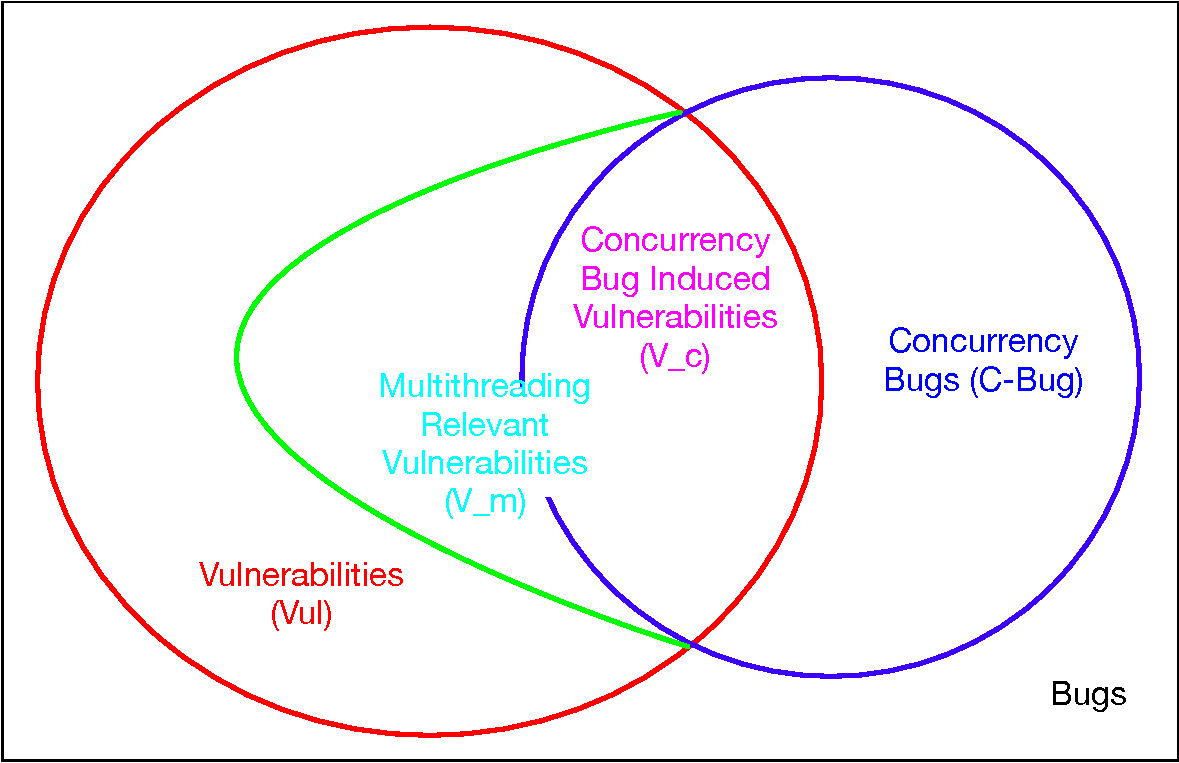
\includegraphics[width=0.75\columnwidth]{res/venn}
	\caption{Venn Diagram of the Multithreading Relevant Vulnerabilities and Bugs}
	\label{fig:venn_con_vul}
\end{center}	
\end{figure}

Multithreading as a popular programming paradigm is an effective way of utilizing multi-core computation resources in modern processors. Meanwhile, the \emph{non-deterministic} behaviors caused by thread-interleavings also pose substantial challenges to vulnerability or bug detection in multithreaded programs~\cite{mtbugs_survey}. On one hand, the interleavings across threads inherently introduce multiple subtle concurrency bugs, e.g., data races, atomic violations, and deadlocks. These bugs can cause undefined program behaviors and sometimes can induce vulnerabilities such as use-after-free (CVE-2016-1972, CVE-2018-5873) and heap-buffer-overflow (CVE-2017-8244), denial-of-service (CVE-2018-0381). On the other hand, as multithreaded programs may accept some inputs, some bugs or vulnerabilities may be difficult or impossible to be triggered with limited initial seed inputs, regardless of whether such bugs are caused by concurrency bugs.


{\noindent\textbf{ Categories of Multithreading-relevant Vulnerabilities and Bugs}\quad} Fig.~\ref{fig:venn_con_vul} depicts the multithreading relevant vulnerabilities and bugs. The rectangle represents all the bugs. The left red circle denotes the vulnerabilities ($Vul$) and the right blue circles denotes the concurrency bugs (\textsf{C-Bug}). The intersection of $Vul$ and \textsf{C-Bug} is the concurrency bug induced vulnerabilities ($V_c$). It may be surprising that there is another category of vulnerabilities $V_m$ which is a proper superset of $V_c$. In fact, there are several vulnerabilities that are tightly relevant with multithreading environment however is not caused by concurrency bugs (\textsf{C-Bug}).

\begin{lstlisting}[language=C,float=ht,caption={An Example Illustrating the vulnerability lies in $V_m$ but not $V_c$.},label={lst:eg_vm}]
int compute(void *s_var) {
    ...
    if (satisfy(s_var)) {
        func_1(s_var);
    } else {
        func_2(s_var);
    }
    ...
}

int main(int argc, char** argv) {
    u8* input = read_file(argv[1]);
    validity_check_1(input);
    pthread_t t1, t2;
    pthread_create(t1, compute, input[0]);
    pthread_create(t2, compute, input[128]);
}	
\end{lstlisting}

In Listing~\ref{lst:eg_vm}, in the multithreading execution environment, if the condition \func{satisfy(s\_var)} returns true, it executes \func{func\_1} otherwise \func{func\_2}; let us suppose that there is a vulnerability inside \func{fun\_2} that is not introduced by concurrency bugs. Note that this branching results may rely on the number of threads, the input content themselves. For example, if in single-threaded mode, \func{satisfy(s\_var)} always returns true, the vulnerability will never be triggered; this vulnerability can only be revealed with more than one thread. Under other circumstances, suppose for the input content, \func{func\_2} will not be executed except for some very specific conditions (e.g., error handling), the vulnerabilities can only be revealed with certain content. Therefore, it may not be enough to only consider the \textsf{C-Bug} induced vulnerabilities $V_c$.


As mentioned in Section~\ref{sec:intro-gbf}, a conventional GBF usually has no awareness of multithreading.
In fact, the only symptom it observes is that a seed has non-deterministic behaviors in that the same seed exercises different traces during calibration execution.
However, since there are \emph{multiple reasons} that can cause non-deterministic behaviors, a GBF typically does not have any countermeasures: all it can do is to increase \Ncal to execute the seeds more times to get more stable running statistics.

When fuzzing a multithreaded program, as long as the seeds can execute the multithreading segments, it always exhibits certain non-deterministic behaviors due to the interleavings across different threads. Compared with the seeds that cannot even entering the multithreading segments, we would \emph{prioritize} these seeds that have thread-interleavings since it is these seeds that 1) may themselves introduce vulnerabilities with different interleavings 2) are more likely to be mutated to seeds that can exercise similar paths~\cite{fuzz_survey}. On the other hand, preserving more multithreading relevant seeds will be more helpful for concurrency bug detectors to detect concurrency violations. Therefore, to enhance the effectiveness of greybox fuzzing on multi-threading programs, we should provide \emph{thread-aware} analyses to help exercise more thread-interleaving paths and generating more multithreading relevant seeds.


We hereby present \mtfuzz, a new greybox fuzzing technique for multithreaded programs.
The core of \mtfuzz is a novel thread-aware seed generation technique which
effectively produces valuable seeds to test the multithreading context. 
\mtfuzz relies on a set of thread-aware instrumentation methods consisting of a
stratified exploration-oriented instrumentation and two complementary instrumentation. The dynamic strategies are hereby optimized for the feedback provided by these instrumentation to improve the effectiveness of fuzzing.

The experimental results demonstrate \mtfuzz significantly outperforms the state-of-the-art greybox fuzzer AFL~\cite{afl} in generating multithreading relevant seeds, detecting multithreading relevant vulnerabilities, and exposing concurrency bugs via generated seeds. In particular, \mtfuzz detected 9 multithreading relevant vulnerabilities and 2 of them have been assigned CVE IDs. Additionally, \mtfuzz helped to expose 19 new concurrency previously bugs with the generated seeds. 

The contributions of this chapter are as follows:
\begin{enumerate}[1)]
\item We designed a novel stratified selective instrumentation strategy specifically designed for exploring thread-interleaving induced paths. This instrumentation significantly increases both the total number of multithreading relevant seeds and its percentage among all generated seeds.
\item We introduced two other thread-aware instrumentations to exhibit more thread-interleavings as well as distinguish overall threading context. This helps increase the thread-interleaving induced coverage during calibration execution, as well as diversify the generated seeds.
\item We integrated the dynamic fuzzing strategies with these thread-aware instrumentations and implemented our enhanced GBF, \mtfuzz, for fuzzing multithreaded programs. To the best of our knowledge, this is the first greybox fuzzer that is optimized for detecting vulnerabilities and concurrency bugs in  multithreaded programs.
\end{enumerate}




\section{Issues in Fuzzing Multithreaded Programs}\label{sec:motivation}

\subsection{A Running Example}\label{sec:example}



\begin{lstlisting}[language=c, float=tp, caption={A program abstracted from real-world multithreaded programs.}, label={lst:eg1},
xleftmargin=.05\columnwidth, xrightmargin=.01\columnwidth,
% xleftmargin=.08\columnwidth, xrightmargin=.03\columnwidth,
% linewidth=.95\columnwidth, 
linebackgroundcolor={%
\ifnum\value{lstnumber}>0\ifnum\value{lstnumber}<3\mtcolor\fi\fi
\ifnum\value{lstnumber}>8\ifnum\value{lstnumber}<12\mtcolor\fi\fi
\ifnum\value{lstnumber}>12\ifnum\value{lstnumber}<14\mtcolor\fi\fi
\ifnum\value{lstnumber}>14\ifnum\value{lstnumber}<16\mtcolor\fi\fi
}]
int g_var=1; %\label{line:g_var_def}%
void inc(int *pv) { *pv += 2; %\label{line:st_mt_func_start}%}

void check(char * msg) {
  if (msg[0] <= '1') exit(1);  %\label{line:st_func_start}%
}

int compute(void *s_var) {
  *s_var += 3; %\label{line:mt_func_start}%
  *s_var *= 2; %\label{line:mt_func_assign}%
  if (*s_var<2) inc(&g_var); %\label{line:mt_func_call}%
  pthread_mutex_lock(&m); %\label{line:mt_func_lock}%
  inc((int*)(s_var)); %\label{line:locked}%
  pthread_mutex_unlock(&m); %\label{line:mt_func_unlock}%
  return *s_var; %\label{line:mt_func_end}%
}

int main(int argc, char **argv) {
  check(argv[1]); %\label{line:main_front}%
  pthread_t T1, T2; %\label{line:main_pthread_t}%
  pthread_create(T1,NULL,compute,argv[1]);  %\label{line:main_thread_fork_1}%
  pthread_create(T2,NULL,compute,argv[1]);  %\label{line:main_thread_fork_2}%
  ...
}
\end{lstlisting}



Listing~\ref{lst:eg1} is a program abstracted from real-world multithreaded programs such as \emph{GraphicsMagick}. Before processing the input, it does a validation check inside \func{check} against some properties of \emph{argv}[1]. if the check fails, the program terminates immediately. The core functionality starts from two threads created at lines \ref{line:main_thread_fork_1} and \ref{line:main_thread_fork_2} respectively in \func{main} function. There are two shared variables: 1) the global variable \var{g\_var} has an initial value 1, 2) and input \var{argv}[1] is passed to both threads T1 and T2 through the thread-forking call to \func{pthread\_create}.
Apparently, there are multiple reads and writes on \var{g\_var} and \var{argv}[1] and this program suffers from data races.


 With this example, we would like to demonstrate that the state-of-the-art GBFs such as AFL can be ineffective in exploring thread-interleaving relevant paths due to \emph{unawareness of multithreading}. 






\subsection{No Strategies to Track Thread-Interleavings}\label{sec:afl_issue_ins}

GBFs such as AFL typically instrument new instructions into the target programs to collect runtime 
coverage information. Specifically, AFL treats the entry instruction of each basicblock 
as the basicblock's \emph{deputy}. From now on, we will 
refer AFL's default selection strategy over the \emph{deputy} instruction as \AFLIns. 
During calibration execution, AFL labels a calculated value to each transition that 
connects the \emph{deputies} of two consecutively executed basicblocks~\cite{afl_detail}. 
By maintaining a set of values for queued seeds, AFL \emph{tracks} the ``coverage'' 
of a PUT. Procedure \emph{cov\_new\_trace} in Algo.~\ref{algo:gbf} is to check whether a value has already been contained in the set.

Fig.~\ref{subfig:transition} depicts the transitions upon executing the functions \func{compute} 
and \func{inc}. For brevity, we use source code to explain the problem and use \emph{statements} to represent the lower level \emph{instructions} in assembly or LLVM IR~\cite{Lattner:2004:LCF:977395.977673}. The arrows denote the transitions between \emph{all} the statements. The pentagons denote the first statements of basicblocks while the other statements are 
represented by rectangles. Since \AFLIns only cares the first statements, only the branching 
edges from \texttt{{if}(s\_var<2)} and the two function call edges to \func{inc} are bookkept
-- these transitions are marked as solid arrows.

\AFLIns works well on single-threaded programs: the kept transitions can reflect both branching conditions (e.g., ``$\texttt{{if}(s\_var<2)}\rightarrow\texttt{inc(\&g\_var)}$'') and the function calls (e.g., ``\texttt{inc((int*)(s\_var))} $\rightarrow $\texttt{*pv+=2}'').
However, in the presence of multithreading, 
it may frequently miss several important transitions of the interleavings between concurrently executed threads. Let us focus on two \emph{different} seeds' execution at two statements: \ding{172}:``\texttt{*s\_var+=3}'' and \ding{173}: ``\texttt{*s\_var*=2}''.  Threads T1 and T2 may execute the two statements with these interleavings: the two T1:\ding{172}$\rightarrow$T2:\ding{172}$\rightarrow$T1:\ding{173}$\rightarrow$T2:\ding{173}, or T1:\ding{172}$\rightarrow$T1:\ding{173}$\rightarrow$T2:\ding{172}$\rightarrow$T2:\ding{173}. After the second \ding{173} is executed the value of \var{*s\_var} is likely to be different; in addition, dependent on the initial value of \var{*s\_var} (propagated from \var{argv[0]}), the condition \texttt{s\_var<2} may also be affected. Therefore, these interleavings may affect subsequent executions and it is expected to keep track of them. However, since AFL only tracks the \emph{deputy-to-deputy} transitions, 
it merely observes that there is a transition from \ding{172}$\rightarrow$\ding{172}.
Since AFL keeps seeds only when it ``sees'' a new transition, it simply discard the second one.
However since the second seed indeed executes a different interleaving, keeping it usually brings positive coverage feedback~\cite{fuzz_survey,ccs18_eval_fuzzing}.
In this sense, it is preferable to apply certain instrumentation to explore more thread-interleaving paths and keep more multithreading relevant seeds.

\subsection{Unawareness of Threading Context}
AFL knows nothing about the threading context, therefore it cannot distinguish whether a transition is from T1 to T2 or from T1 to T1. For example, as to the (four) interleavings that can occur when executing \ding{172} and \ding{173}, AFL is only aware of \ding{172}$\rightarrow$\ding{172}. Since such a transition can also happen when \ding{172} is inside a loop, AFL may think this is not a ``new'' transition. Furthermore, the threading information does help to provide additional feedback that is orthogonal to the transitions between the deputy instructions. In this sense, we should provide a strategy to record the threading context.



\begin{figure}[t]
	\centering
	\begin{subfigure}[b]{.38\columnwidth}
		\centering{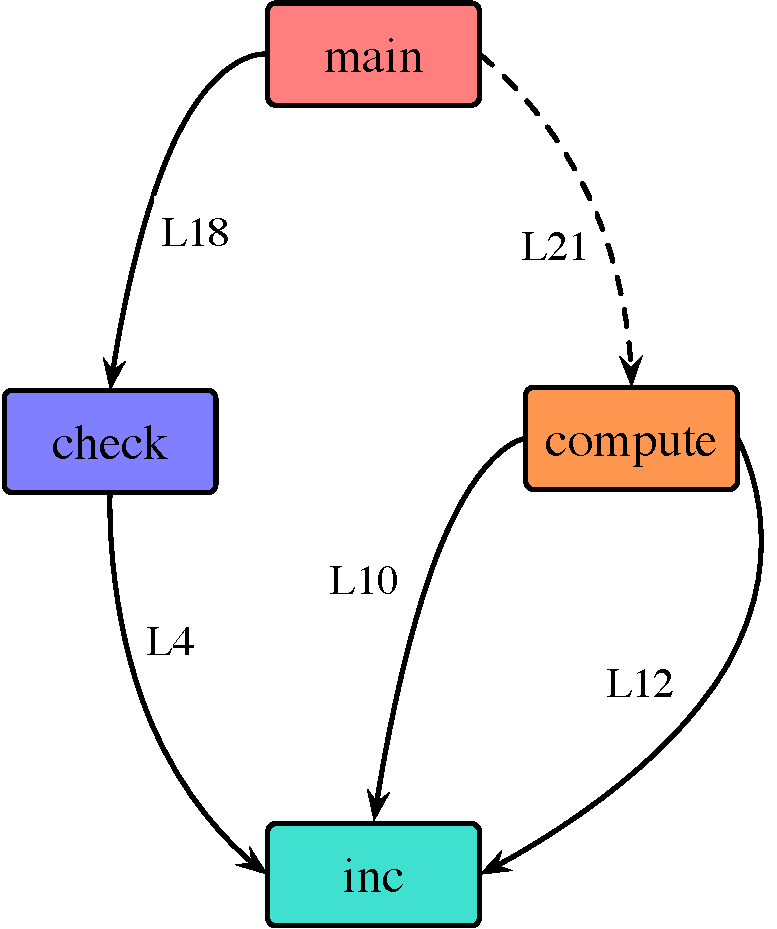
\includegraphics[width=.8\linewidth]{res/mtfuzz/callgraph.pdf}}
\caption{}\label{subfig:callgraph}
	\end{subfigure}\begin{subfigure}[b]{0.61\linewidth}
		\centering{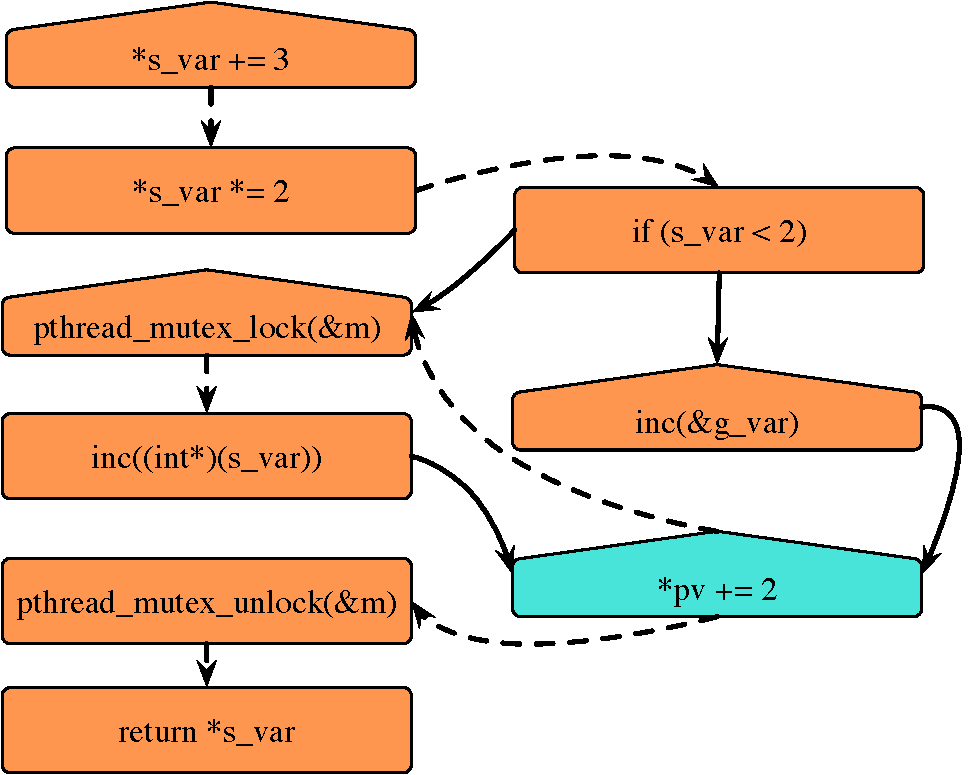
\includegraphics[width=.75\linewidth]{res/mtfuzz/transitions.pdf}}
\caption{}\label{subfig:transition}
	\end{subfigure}
	\caption{Thread-aware Callgraph (\ref{subfig:callgraph}) of Listing~\ref{lst:eg1} and its edge transitions in functions \texttt{compute} and \texttt{inc} (\ref{subfig:transition}).}
	\label{fig:eg_details}
\end{figure}





\begin{figure*}[ht]
    \centering
    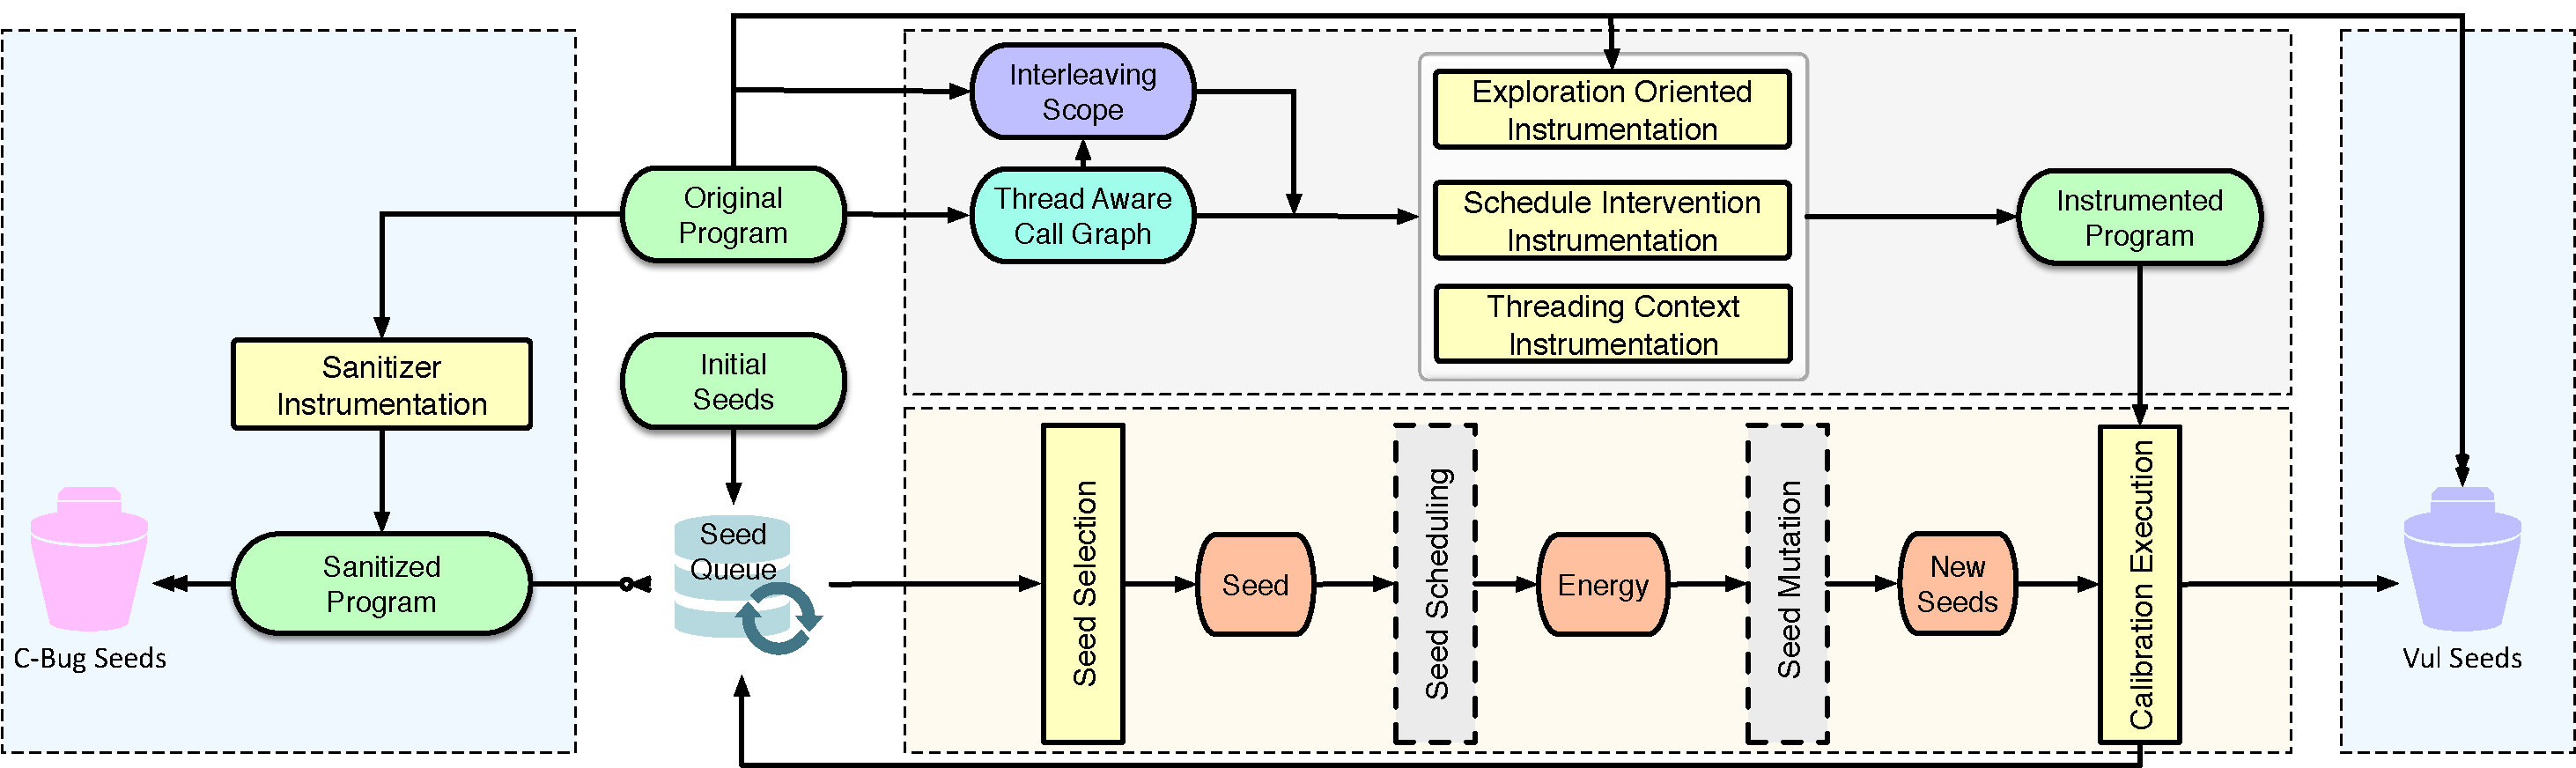
\includegraphics[width=0.93\textwidth]{res/mtfuzz/overview.pdf}
    \caption{Overall workflow of \mtfuzz.}
    \label{fig:workflow}
\end{figure*} 
\subsection{Low Diversity across Executions}\label{sec:afl_issue_mt}
When encountering a non-deterministic behavior seed, the only strategy of AFL is to execute the seeds more times. However, since the calibration execution is applied \emph{continuously} \Ncal times, the systematic level environment such as CPU usage, memory consumption, or other I/O status is prone to be similar~\cite{posixstd,tlpi}. This will decrease the entropy to diversify the actual scheduling. For example, in a calibration execution with $\Ncal=40$,  T1:\ding{172}$\rightarrow$T2:\ding{172}$\rightarrow$T1:\ding{173}$\rightarrow$T2:\ding{173} and T2:\ding{172}$\rightarrow$T1:\ding{172}$\rightarrow$T2:\ding{173}$\rightarrow$T1:\ding{173} may occur 15 and 20 times respectively, however interleavings such as T1:\ding{172}$\rightarrow$T1:\ding{173}$\rightarrow$T2:\ding{172}$\rightarrow$T2:\ding{173} only occurs 5 times, while there is no T2:\ding{172}$\rightarrow$T2:\ding{173}$\rightarrow$T1:\ding{172}$\rightarrow$T1:\ding{173} at all. In addition, since the running statistics are collected during calibration execution, this would also affect the decision in seed triaging. Ideally, we would like to keep as many distinct interleavings as possible since that marks the potential interleavings a seed can exhibit with different scheduling priorities.



\subsection{Our Solutions}
In order to improve the effectiveness of fuzzing multithreaded programs, we propose the following solutions.
\begin{enumerate}[{\bf S1}]
    \item Instead of equally choosing the the entry instruction of a basicblock as the deputy instruction, we apply a stratified exploration-oriented instrumentation by distinguish whether an instruction may happen-in-parallel with others~\cite{DBLP:conf/ppopp/DiS16,DBLP:conf/cgo/SuiDX16}.
This helps the fuzzer to track more thread-interleaving transitions.
    \item We instrument at the call site of thread-forking, locking, unlock, joining APIs and collect the thread and deputy instruction information to calculate the overall threading context per execution. This information is utilized to diversify the threading context of the seeds in the queue.
    \item We instrument at the entry of a thread start routine function a segment that can dynamically adjust the thread priority. It aims to increase the interleaving diversity during calibration execution.
\end{enumerate}



 \section{System Overview}

Fig.~\ref{fig:workflow} depicts the overall workflow of \mtfuzz. It contains three major components: (1) static-analysis-guided instrumentation (shown in the \emph{top center} area), (2) dynamic fuzzing (shown in the \emph{bottom center} area), and (3) concurrency bug replay (shown in the \emph{left and right} area). During instrumentation (~\S~\ref{sec:instrument}), we firstly compute the thread-aware ICFG (interprocedural control-flow graph) in \S~\ref{sec:tcg} for a multithreaded program (\ProgO). Based on this ICFG, we perform three categories of instrumentation: the one focusing on exploring more multithreading relevant paths (\S~\ref{sec:instrument_explore}), the one aiming to intervene the thread scheduling (\S~\ref{sec:instrument_schedule}) and the one that provides the threading context (\S~\ref{sec:instrument_thread_ctx}) to eventually produce the instrumented program~\Prog. During dynamic fuzzing~\S~\ref{sec:fuzz}, based on the instrumentation feedback, we apply seed selection (\S~\ref{sec:seed_select}), calibration execution (\S~\ref{sec:calibrate}) and seed triaging (\S~\ref{sec:seed_save}) that are turned for generating multithreading relevant seeds. Since the fuzzing procedure can only detect \emph{vulnerabilities} that are resulted from crashed seeds, we need a concurrency bug detector to replay with the generated seeds to see whether they can trigger certain concurrency violations; this will be covered in the evaluation section (\S~\ref{sec:eval_overall}).

\section{Static Instrumentation}\label{sec:instrument}
The instrumentation is used to provide the thread-aware information for fuzzing.

As discussed in \S\ref{sec:afl_issue_mt}, the instrumentation strategy in existing GBFs is thread-unaware, which may miss transitions that caused by thread-interleaving for triggering vulnerabilities in multithreaded programs. Drawn from this insight, the precise fuzzing should distinguish program statements that may be access by concurrent threads, which requires ``finer-grained'' instrumentation to pay attention to the seeds that can capture the instruction transitions caused by interleaved threads, while deprioritize the seeds that exercise new paths only within a single thread.
We use results from static context-sensitive may-happen-in-parallel analysis~\cite{DBLP:conf/cgo/SuiDX16} to determine the thread-interleaving scope. The pointer analysis and lock analysis are enabled to further refine the scope in order to filter out the interleaving-free statements.
The static analysis is adopted as the preprocessing in~\S\ref{sec:preprocess} for our three categories of  instrumentation (\S~\ref{sec:instrument_explore}-\S~\ref{sec:instrument_thread_ctx}) for exploring new coverage, for intervening the schedule, and for guiding the seed selection procedure. 


\subsection{Preprocessing}\label{sec:preprocess}

\subsubsection{Thread-aware ICFG Generation}\label{sec:tcg}
We firstly apply Andersen's inclusion-based pointer analysis~\cite{Andersen94programanalysis} on the target program. The points-to results are used to resolve indirect calls to eventually produce an interprocedural control-flow graph (ICFG). By taking into account the semantics of pthread APIs, we get an ICFG that is aware of the following multithreading information:
\begin{enumerate}[(1)]
    \item \TStart is the set of program sites that call thread-forking functions. This includes the explicit call to \func{pthread\_create}, or the \func{std::thread} constructor that internally uses \func{pthread\_create}, etc. These called functions, denoted as \FSStart, are extracted from the semantics of these forking sites.
\item \TEnd contains call sites for functions that mark the end of a multithreading execution. It includes the call sites of the pthread APIs such as \func{pthread\_join}, \func{pthread\_cancel}, \func{pthread\_exit}, etc.
    \item \TLock is the set of sites that call thread-locking functions such as \func{pthread\_mutex\_lock}, \func{pthread\_mutex\_trylock}, etc.
\item \TUnLock is the set of sites calling thread-unlocking functions such as \func{pthread\_mutex\_unlock} and \func{pthread\_rwlock\_unlock}.
    \item \TSharedVar is the set of variables that \emph{may be} shared among different threads. This includes the global variables and those variables that are passed from the threading fork sites \TStart.
\end{enumerate}

\subsubsection{Suspicious Interleaving Scope Extraction}\label{sec:extract}
Given a program that may run with multiple threads, we would prefer the instrumentation to collect various traces to reflect the interleavings. However, instrumentation always brings execution overhead to original programs, especially when adopting an intensive instrumentation strategy to cover all concerned sites.  Owing to the static information provided by the thread-aware ICFG in~\S\ref{sec:preprocess}, we know that multithreading interleavings may only happen on \emph{certain} program statements. We hereby use \mtiscope to denote the set of these statements and name it as \emph{suspicious interleaving scope}. Thus, the instrumentation is targeted on these statements. A statement $l$ is added into an thread-interleaving scope if there exists another statement $l'$, which may happen-in-parallel with $l$ and may access the same memory inferred by the pointer analysis, but not protected by the same lock.




In Listing~\ref{lst:eg1}, $\FSStart=\{\func{compute}\}$ based on the function call at Lines~\ref{line:main_thread_fork_1} and \ref{line:main_thread_fork_2}. We then get all the functions that may be (directly or indirectly) called by functions inside \FSStart, i.e., $\{inc, compute\}$ and the scope \mtiscope comes from Lines~\ref{line:g_var_def}, \ref{line:st_mt_func_start},
\ref{line:mt_func_start}$\sim$\ref{line:mt_func_end}.
We exclude the statements that do not access or modify the shared variables ${g\_var1}$, ${g\_var2}$, ${s\_var}$, 
which means we should exclude Lines~\ref{line:mt_func_lock} and \ref{line:mt_func_unlock}. In the end, the scope is determined as $\mtiscope=\{\ref{line:g_var_def},\ref{line:st_mt_func_start},
\ref{line:mt_func_start},\ref{line:mt_func_assign},\ref{line:mt_func_call},\ref{line:locked},\ref{line:mt_func_end}\}$. It is worth noting that line $\ref{line:locked}$ \emph{is} inside $\mtiscope$ since it may happen-in-parallel with lines~\ref{line:mt_func_start} and ~\ref{line:mt_func_assign}.


\subsection{Exploration-Oriented Instrumentation}\label{sec:instrument_explore}
With the knowledge of \mtiscope, we are able to instrument more stubs on these instructions inside the scope than the others, for exploring new ``transitions''. However, it is \emph{impractical} to instrument intensively on \emph{each instruction} inside \mtiscope since this still may greatly reduce the overall performance. It is also \emph{unnecessary} to do so --- although theoretically interleavings may happen everywhere at each instruction inside \mtiscope, in practice several instructions in one thread can still be executed subsequently. This means that we can skip some instructions for instrumentation, or instrument the instructions \emph{with a probability}.
We still need to instrument on the other parts of the program in case that the initial seeds do not cover the multithreading statements at all. Hence, we need the instrumentation to help explore more \emph{new} traces. Also similarly, we can \emph{skip} instrumentation on some instructions with certain probabilities.

\subsubsection{Instrumentation Probability Calculation}
We first calculate a \emph{base instrumentation probability} according to cyclomatic complexity. We use this since it has been demonstrated that bugs or vulnerabilities usually come from functions that have higher cyclomatic complexity~\cite{macabecc,vul_metric,fuzz_vul_metric}. For each function $\aFUNC$, we firstly calculate the complexity value: $M_c(\aFUNC) = E(\aFUNC) - N(\aFUNC) + 2$ where $E(\aFUNC)$ is the basicblock edge number of the function, $N(f)$ is the number of basicblocks. Intuitively, this value indicates the complexity of the function across its basicblocks. As 10 is considered to the preferred upper bound~\cite{macabecc}, we determine the base probability as
\begin{equation}
    \ccr{\aFUNC} = \min\big\{\frac{E(\aFUNC)-N(\aFUNC)+2}{10}, ~1.0\big\}
\end{equation}
We use $\stpn$ as the probability to \emph{selectively} instrument on the first instruction of a basicblock that is \emph{totally} outside the scope of multithreading environment, i.e., \emph{none of} the instructions inside this basicblock belongs to \mtiscope.
\begin{equation}
    \stp{\aFUNC} = \min\big\{\ccr{\aFUNC}, ~\stpnO\big\}
\end{equation}
where $0<\stpnO<1$. Empirically, we set $\stpnO=0.5$.

On the other hand, for each basicblock \aBB inside the given function~\aFUNC, we calculate the total number of instructions $N(\aBB)$, and the total number of memory operation instructions  $N_m(\aBB)$, e.g., load/store operations, or builtin memory function calls such as \func{memcpy}, \func{strncat}, \func{malloc}, \func{free}, etc. 
Then for each of the instructions, we instrument based on the probability as:
\begin{equation}
    \mtp{\aFUNC}{\aBB} = \min\big\{\ccr{\aFUNC}\cdot\frac{N_m(\aBB)}{N(\aBB)}, ~\mtpnO \big\}\end{equation}
where $\mtpnO$ is a factor satisfying $0<\mtpnO<1$ and defaults to $0.33$.

\subsubsection{Instrumentation Algorithm}
The exploration-oriented instrumentation algorithm is described in Algo.~\ref{algo:inst_explore}. It iterates each function inside a program. For each basicblock \aBB in function \aFUNC, we firstly get the intersection of the instructions inside \aBB and \mtiscope. If this intersection \mtiscope(\aBB) is empty, it instruments the \emph{first instruction} of \aBB with a probability of \emph{\stpn(\aFUNC)}. Otherwise, for the first instruction in \aBB, we always instrument it (instrument with probability of 1.0); for the other instructions, if they are inside \mtiscope, we instrument them with a probability of \mtp{\aFUNC}{\aBB}. We will refer our selection of deputy instructions as \MTIns.

\begin{algorithm}[t]
  \SetKwInOut{Input}{input}
  \SetKwInOut{Output}{output}
\Input{Target program \var{P}, suspicious interleaving scope~\mtiscope}\Output{Program \var{P} instrumented with exploration stubs}
\For{\var{\aFUNC} $\in$ \var{P}}{
  \For{\var{\aBB} $\in$ \aFUNC}{
    $\mtiscope(\aBB) = \mtiscope\cap~\aBB$\;
    \uIf{$\mtiscope(\aBB)~!\!=\emptyset$}{
      \For{\aINSTR $\in$ \aBB}{
        \uIf{\func{is\_first\_instr(\aINSTR, \aBB)}}{
          exploration\_instrument(\aINSTR, 1.0)\;
        }
        \ElseIf{$\aINSTR\in\mtiscope$}{
          exploration\_instrument\big(\aINSTR, \mtp{\aFUNC}{\aBB}\big)\;
        }
      }      
    }\Else{
      \For{\aBB $\in$ \aFUNC}{
        \aINSTR = get\_first\_inst(\aBB)\;
        exploration\_instrument\big(\aINSTR, \stp{\aFUNC}\big)\;
      }
    }
  }
}
\caption{Exploration-Oriented Instrumentation}\label{algo:inst_explore}
\end{algorithm}

\subsubsection{Properties of the Coverage in \MTIns}

First, for both \AFLIns and \MTIns, the coverage is shaped by the transitions between deputy instructions. The difference is that we use a stratified instrumentation strategy to focus on the interleavings introduced by multithreading scheduling. Compared to \AFLIns, \MTIns instruments less on the single threading program statements, while applies more instrumentation to explore more interleavings across different threads with certain probabilities.

Second, mistakenly instrumenting on non-entry instructions that are not in \mtiscope will \emph{only introduce runtime overhead}, but \emph{never} help to keep more seeds.
This can be proved by the fact that GBFs keep new seeds based on ``new transitions'', however the ``new transitions'' conditions are always the regardless of whether the exercised instruction are instrumented. 
In this sense, we may expect that there will not be seeds \emph{accidentally} added into the seed queue due to over-estimation of \mtiscope. 

Thirdly, \MTIns's strategy to tracking multithreading interleaving \emph{is} useful and it is worth instrumenting more on these instructions that may be executed parallelly with other instructions. The major reason is that we can expect to have more valuable seeds. Same as other GBFs, we still rely on observations of ``new transitions'' to keep seeds, and \MTIns tends to keep more seeds that execute thread-interleaving, regardless of the precision of the calculated \mtiscope. First, it means that more seeds in the seed queue for fuzzing have executed the multithreading code segments, instead of having failed the validation check quite earlier. Hence, these seeds can execute the ``deeper part'' of a multithreaded program. When they are mutated, compared with those seeds that fail the validity check, there is a higher chance that the newly generated seeds from these seeds also pass the check and exercise different part of the multithreading segments. Therefore, the high ratio of seeds that can execute multithreading segments already indicates the seeds are probably of high qualities. Second, since seeds usually exhibit some preference in executing with certain interleavings, some thread-interleavings are more ``stable'', they may be just like the regular transitions inside single thread.

Finally, since \MTIns only selectively instruments the instructions inside \mtiscope with a probability of at most \mtpnO, we avoid over-emphasizing thread-interleaving induced transitions, as well as seek a balance between runtime instrumentation overhead and coverage feedback. 





\subsection{Schedule Intervention Instrumentation}\label{sec:instrument_schedule}

Without specifying any schedule policy or priority, the operation systems usually determine the actual schedule dynamically~\cite{tlpi,posixstd}. As mentioned in \S\ref{sec:afl_issue_mt}, without scheduling intervention the calibration execution during fuzzing may not exhibit diverse interleavings, which is unsatisfactory for covering new transitions. 

POSIX compliant systems such as Linux
usually provide the APIs to control the low level process or thread scheduling~\cite{posixstd,tlpi}.
In order to intervene the interleavings during the execution of the multithreaded program, we adjust the thread priorities.
This heavily resorts to the POSIX API \func{pthread\_setschedparam}. Our intervention of scheduling follows two principles: 1) the intervened schedule should be possible to happen in reality without this intervention; 2) the schedule should make the interleavings more diverse. We therefore instrument a function call \rtifunc at the start of the thread routine. This instrumented function does two things:
\begin{enumerate}[(1)]
    \item For each newly mutated test input, it calls \func{pthread\_self} in the entry of \FSStart to collect the runtime thread IDs. This serves two purposes.
    First, it marks the entering of the multithreading region in order to inform the fuzzer that the execution trace has covered the thread spawning statements.
    Second, each collected thread ID will also be associated with a unique number \ntid starting from $1,2,\ldots$, which will be used to calculate the threading context in \S\ref{sec:instrument_thread_ctx}.
    \item During the calibration execution~\S~\ref{sec:calibrate}, whenever the thread comes to call \rtifunc, it changes the schedule policy to \emph{SCHED\_RR}, and assigns a \emph{ranged random value} to its priority.
    We make the priority value to be \emph{uniformly distributed random} in order to diversify the combinations among threads.
\end{enumerate}

\subsection{Threading Context Instrumentation}\label{sec:instrument_thread_ctx}
We also apply an instrumentation to track the threading context, which is used to collect thread relevant context for additional feedback during seed selection.
This context is collected at the call site of $\FSThread=\{\TLock, \TUnLock, \TEnd\}$, each of which has the form $\threadCtxn=\threadCtx{\iloc}{\ntid}$. Here \iloc is the labeling value of previous deputy instruction (c.f. \S\ref{sec:afl_issue_ins} and \S~\ref{sec:instrument_explore}). \ntid is obtained by getting the value of the key identified by current thread ID from the thread ID map collected at \S\ref{sec:instrument_schedule}. For each function in \FSThread, we keep a sequence of context $\langle\threadCtxn{_1}(f),\ldots,\threadCtxn{_n}(f)\rangle$,$f\in\FSThread$; and at the end of each execution we calculate a hash value $H(f)$ for each of them. The tuple $\tctxSign=\big\langle H(\TLock),H(\TUnLock),H(\TEnd)\big\rangle$ is a \emph{context signature} that determines the overall threading context of a specific execution. Essentially, this is a sampling on these thread relevant APIs to track the overall thread information and transitions of a particular run. As we shall see later, this plays an important role in seed selection (\S\ref{sec:seed_select}).

Till now, we have done all the static instrumentation. Note that we manage to keep the original programs' semantics, and hence the execution behaviors are basically the same as the original one.

\section{Dynamic Fuzzing}\label{sec:fuzz}
The dynamic fuzzing loop follows a typical GBF procedure as described in Algo.\ref{algo:gbf}. We improve the procedures of seed selection (\S\ref{sec:seed_select}),
calibration execution (\S\ref{sec:calibrate}) and seed triaging (\S\ref{sec:seed_save}) to fit specially for fuzzing multithreaded programs, based on the instrumentation information provided in \S\ref{sec:instrument}.

\subsection{Seed Selection}\label{sec:seed_select}

Seed selection decides which seeds to be mutated next. In practice, this problem is reduced to whether the next seed $t$ at the queue header will be selected into $\Seeds$, which is depicted by Algo.~\ref{algo:select_seed}.






During seed selection, in addition to following AFL's strategy by using \func{has\_new\_trace(\Seeds)} to  checking whether \Seeds contains a ``favored seed'' $t$ that covers a new transition (\func{cov\_new\_trace(t)}=true), we also check whether there is at least one seed in \Seeds that reaches the multithreading code (i.e., \func{has\_new\_mt\_ctx(\Seeds)}). If either of the conditions is satisfied, it means there are some ``interesting'' seeds.
Specifically, if the seed has a new threading context, the algorithm directly returns  true. If it covers a new trace, it has a probability of \probYNT to be selected; otherwise, the probability is \probYNN. Last, if no interesting seeds in \Seeds are interesting at all, the algorithm selects with a probability of \probNNN. Analogous to AFL's selection strategy, we set $\probYNT=0.95$, $\probYNN=0.01$, $\probNNN=0.15$.

To implement $\func{cov\_new\_mt\_ctx(t)}$, we track the context of calling a multithreading API in $\FSThread=\{\TEnd, \TLock, \TUnLock\}$ (c.f. \S\ref{sec:instrument_thread_ctx}) and check whether the  context signature \tctxSign has been met before ---  when \tctxSign is new, $\func{cov\_new\_mt\_ctx(t)}=true$; otherwise, $\func{cov\_new\_mt\_ctx(t)}=false$. Note that $\func{cov\_new\_trace(t)=true}$ does not imply $\func{cov\_new\_mt\_ctx(t)=true}$. The reason is that (1) we cannot instrument inside the body of thread API functions in \FSThread, and hence $\func{cov\_new\_trace}$ cannot track the transitions; (2) $\func{cov\_new\_mt\_ctx}$ also depends on the thread IDs that $\func{cov\_new\_trace}$ is unaware of.  




\begin{algorithm}[t]
\SetKwInOut{Input}{input}
  \SetKwInOut{Output}{output}
  \Input{Seed queue~\Seeds, current seed in queue $t$}
  \Output{whether $t$ will be selected in this round}
  \uIf{has\_new\_mt\_ctx(\Seeds) \textsc{or} has\_new\_trace(\Seeds)}{
      \uIf{cov\_new\_mt\_ctx($t$)}{
        \Return{true}\;
      } \uElseIf{\func{cov\_new\_trace($t$)}}{
        \Return{\func{select\_with\_prob(\probYNT)}}\;
      } \Else{
        \Return{\func{select\_with\_prob(\probYNN)}}\;
      }
  }\Else{
    \Return{\func{select\_with\_prob(\probNNN)}}\;
  }
  \caption{Algorithm to Select Next Seed}\label{algo:select_seed}
\end{algorithm}


\subsection{Calibration Execution}\label{sec:calibrate}
Multithreaded programs introduce non-deterministic behaviors when different interleavings are involved.
As seen in Algo.~\ref{algo:gbf}, for a mutated seed, a GBF typically executes the PUT with multiple times. 
Owing to~\rtifunc, we are now able to tell whether the current non-deterministic behavior is relevant with a multithreading execution. In fact, since we focus on multithreading only, based on the times of the threading forking operations the fuzzer has observed, the fuzzer can distinguish the calibration on those seeds that have non-deterministic behaviors purely by checking whether the execution traces have touched the threading relevant regions. Further, if we know that a seed may have more distinct values of \tctxSign (the number of distinct values for seed $t$ is denoted as \Nmt(t)), there will be more interleavings. To determine the calibration times~\Ncal, we rely on \Nmt. In AFL, the calibration times is calculated by the equation below:
\begin{equation}
    \Ncal(t) = \NcalO + \NcalV\cdot\NcalB \label{eq:afl_cal}
\end{equation}
where \NcalO is the initial calibration times, \NcalV is a constant as the ``bonus'' calibration times for non-deterministic runs, and $\NcalB\in\{0,1\}$. \NcalB=0 if none of the \NcalO calibration runs show non-deterministic behaviors, otherwise \NcalB=1. We argue this to specially fit for multithreading setting. 
\begin{equation}
    \Ncal(t) = \NcalO + \texttt{min}\big\{\NcalV, \NcalO\cdot\Nmt(t)\big\}
\end{equation}
In both AFL and \mtfuzz, $\NcalO=8$, $\NcalV=32$.
For all the \Ncal calibration runs, we track their execution traces and count how many different traces (\NcalTrace) it exhibits. 


\subsection{Seed Triaging}\label{sec:seed_save}
This handles how to categorize the seeds after calibration execution. \mtfuzz still follows the workflow at Lines~\ref{line:algo:triage_start}$\sim$\ref{line:algo:triage_end} in Algo.~\ref{algo:gbf}: if there is a crash, we mark these seeds as vulnerable; if the seed covers new transitions, we append it to the queue. One major difference is that these ``seemingly normal'' seeds may actually have concurrent bugs. These will be handled in the replaying procedure (\S~\ref{sec:eval_overall}) after fuzzing. To provide a hint on how many times to be executed on a specific seed during replaying, we keep \NcalTrace statistics.



\begin{table*}[ht]
\caption{Static information of the 12 evaluated programs.}
\label{tbl:bm_stats}
\begingroup
\setlength{\tabcolsep}{0pt} % Default value: 6pt
\renewcommand{\arraystretch}{0.9} % Default value: 1
\scriptsize
\begin{tabular}{c"c|c|c|c"c|c|c|c|r}
\thickhline
\textbf{ID} &\textbf{Project} & \textbf{MT Type} & \textbf{Command Line Options}  & \textbf{\begin{tabular}[c]{@{}c@{}}Binary\\ Size\end{tabular}} &  \textbf{$T_{pp}$} & \textbf{$N_{B}$} & \textbf{$N_{I}$} & \textbf{$N_{ii}$} & \textsf{$\frac{N_{ii}-N_{B}}{N_{B}}$} \\ \thickhline
\textbf{lbzip2-c} & lbzip2-2.5 & native & \pbin{lbzip2} -k -t -9 -z -f -n4 FILE & 377k & 7.1s & 4010 & 24085 & 6208 & 54.8\% \\  \hline
\textbf{pbzip2-c} & pbzip2-v1.1.13 & native & \pbin{pbzip2} -f -k -p4 -S16 -z FILE & 312k & 0.9s & 2030 & 8345 & 2151 & 6.0\% \\  \hline
\textbf{pbzip2-d} & pbzip2-v1.1.13 & native & \pbin{pbzip2} -f -k -p4 -S16 -d FILE & 312k & 0.9s & 2030 & 8345 & 2151 & 6.0\% \\ \hline
\textbf{pigz-c} & pigz-2.4 & native & \pbin{pigz} -p 4 -c -b 32 FILE & 117k & 5.0s & 3614  & 21022 & 5418 & 49.9\% \\ \hline
\textbf{pxz-c} & pxz-4.999.9beta & OpenMP & \pbin{pxz} -c -k -T 4 -q -f -9 FILE & 42k & 1.2s & 3907 & 30205 & 7877 & 101.6\% \\ \hline
\textbf{xz-c} & XZ-5.3.1alpha & native & \pbin{xz} -9 -k -T 4 -f FILE & 182k & 8.4s & 4892 & 34716 & 8948 & 82.9\% \\ \hline
\textbf{gm-cnvt} &  GraphicsMagick-1.4 & OpenMP & \pbin{gm} convert -limit threads 4  FILE out.bmp & 7.6M & 224.4s & 63539 & 383582 & 98580 & 55.1\% \\ \hline
\textbf{im-cnvt} & ImageMagick-7.0.8-7 & OpenMP & \pbin{convert} -limit thread 4 FILE out.bmp & 19.4M & 434.2s & 128359 & 778631 & 200108 & 55.9\% \\ \hline
\textbf{cwebp} & libwebp-1.0.2 & native & \pbin{cwebp} -mt FILE -o out.webp & 1.8M & 56.3s & 12117 & 134824 & 33112 & 173.3\%\\ \hline
\textbf{vpxdec} & libvpx-v1.3.0-5589 & native & \pbin{vpxdec} -t 4 -o out.y4m FILE & 3.8M & 431.6s & 31638 & 368879 & 93400 & 195.2\% \\ \hline
    \textbf{x264} & x264-0.157.2966 & native & \pbin{x264} --threads=4 -o out.264 FILE & 6.4M & 1701.0s & 38912 & 410453 & 103926 & 167.1\% \\ \hline
\textbf{x265} & x265-3.0\_Au+3 & native & \pbin{x265} --input FILE --pools 4 -F 2 -o & 9.7M & 78.3s & 22992 & 412555 & 89408 & 288.9\% \\ \thickhline
\end{tabular}
\endgroup
\end{table*}



\begin{table}[h]
\caption{Fuzzing and Replaying Results on \AFL, \mtfuzzc, and \mtfuzz}
\label{tbl:eval_overall}
\centering
\footnotesize
\begin{tabular}{|c|c|c|c|c|c|c|c|c|}
\thickhline
\multicolumn{2}{|c|}{\multirow{2}{*}{\textbf{ID}}} & \multicolumn{3}{c|}{\textbf{Gen Tests}} & \multicolumn{3}{c|}{\textbf{Vuls}} & \multirow{2}{*}{\textbf{C-Bugs}} \\ \cline{3-8}
\multicolumn{2}{|c|}{} & \textbf{\testsALL} & \textbf{\testsMT} & \textbf{\textbf{\testsRatio}}  & \textbf{\vulsNUM} &  \textbf{\vulsMT} & \textbf{\vulsST} &  \\ \hline
\multirow{12}{*}{\textbf{\mtfuzz}}  & \textbf{lbzip2-c} &  3350   & 753   &  22.5\%  &  0   & 0 & 0 & 1   \\ \cline{2-9} 
    & \textbf{pbzip2-c} &  175    & 50    &  28.6\%  &  0   & 0 & 0 & 0    \\ \cline{2-9} 
    & \textbf{pbzip2-d} &  926    & 7     &  0.8\%   &  0   & 0 & 0 & 0  \\ \cline{2-9} 
    & \textbf{pigz-c} &  737    & 592   &  80.3\%  &  0   & 0 & 0 & 1   \\ \cline{2-9} 
    & \textbf{pxz-c} &   2305   & 958   &  41.6\%  &  0   & 0 & 0 & 0  \\ \cline{2-9} 
    & \textbf{xz-c} &  1327   & 257   &  19.4\%  &  0   & 0 & 0 & 0  \\ \cline{2-9} 
    & \textbf{gm-cnvt} &  3921   & 1872  &  47.7\%  &  0   & 0 & 0 & 3 \\ \cline{2-9} 
    & \textbf{im-cnvt} &  3289   & 2460  &  74.8\%  &  8   & 2 & 1 & 2  \\ \cline{2-9} 
    & \textbf{cwebp} &  4755   & 2234  &  47.0\%  &  9   & 0 & 1 & 0  \\ \cline{2-9} 
    & \textbf{vpxdec} &  13046  & 3117  &  23.9\%  &  345 & 1 & 2 & 1  \\ \cline{2-9} 
    & \textbf{x264} &  4465   & 4252  &  95.2\%  &  3   & 1 & 0 & 4  \\ \cline{2-9} 
    & \textbf{x265} &  6420   & 4701  &  73.2\%  &  \gres{49}  & 0 & 1 & 0  \\ \thickhline
\multirow{12}{*}{\textbf{\mtfuzzc}}    & \textbf{lbzip2-c} &  4155   &  1352  &  32.5\%  & 0   & 0 & 0 & 1  \\ \cline{2-9}
    & \textbf{pbzip2-c} &  227    &  59    &  26.0\%  & \gres{6}   & \gres{1} & 0 & 0   \\ \cline{2-9}
    & \textbf{pbzip2-d} &  982    &  11    &  1.2\%   & 0   & 0 & 0 & 0   \\ \cline{2-9}
    & \textbf{pigz-c} & \gres{921  } & \gres{789 } & \gres{85.7\%} &  0    &   0   &   0 & 1  \\ \cline{2-9}
    & \textbf{pxz-c} &  2804   &  1675  &  59.7\%  & 0   & 0 & 0 & 0  \\ \cline{2-9}
    & \textbf{xz-c} &  1359   &  268   &  19.7\%  & 0   & 0 & 0 & 0  \\ \cline{2-9}
    & \textbf{gm-cnvt} & \gres{4677 } & \gres{3265} & \gres{69.8\%} &  0    &   0   &   0 & \gres{5} \\ \cline{2-9}
    & \textbf{im-cnvt} &  4036   &  2092  &  51.8\%  & 0   & 0 & 0 & 4  \\ \cline{2-9}
    & \textbf{cwebp} &  5549   &  3095  &  55.8\%  & \gres{11}  & 0 & 1 & 0  \\ \cline{2-9}
    & \textbf{vpxdec} &  13927  &  3302  &  23.7\%  & \gres{364} & 1 & 2 & 1  \\ \cline{2-9}
    & \textbf{x264} &  4457   &  4197  &  94.2\%  & 6   & 1 & 0 & 6  \\ \cline{2-9}
    & \textbf{x265} &  \gres{6743} & {5007}  &  74.3\%  & 43  & 0 & 1 & 0  \\ \thickhline
\multirow{12}{*}{\textbf{\AFL}}    & \textbf{lbzip2-c} & \gres{4503 } & \gres{1637} & \gres{36.4\%} &  0    &   0   &   0 & 1   \\ \cline{2-9}
    & \textbf{pbzip2-c} & \gres{253  } & \gres{78  } & \gres{30.8\%} &  4    &   \gres{1}   &  0 & 0   \\ \cline{2-9}
    & \textbf{pbzip2-d} & \gres{1231 } & \gres{47  } & \gres{3.8\% } &  \gres{5}    &   \gres{1} & 0  & 0  \\ \cline{2-9}
        & \textbf{pigz-c} & \gres{921  } & \gres{789 } & \gres{85.7\%} &  0    &   0   &   0 & 1  \\ \cline{2-9}
    & \textbf{pxz-c} & \gres{3658 } & \gres{2523} & \gres{69.0\%} &  0    &   0   &   0 & 0  \\ \cline{2-9}
    & \textbf{xz-c} & \gres{1598 } & \gres{493 } & \gres{30.9\%} &  0    &   0   &   0 & 0  \\ \cline{2-9}
    & \textbf{gm-cnvt} & \gres{4677 } & \gres{3265} & \gres{69.8\%} &  0    &   0   &   0 & \gres{5} \\ \cline{2-9}
    & \textbf{im-cnvt} & \gres{4355 } & \gres{3671} & \gres{84.3\%} &  \gres{21} &  \gres{4} &  1 & \gres{3}  \\ \cline{2-9}
    & \textbf{cwebp} & \gres{5701 } & \gres{3347} & \gres{58.7\%} &  8    &   0   &   1 & 0  \\ \cline{2-9}
    & \textbf{vpxdec} & \gres{14665} & \gres{3656} & \gres{24.9\%} &  336  &   \gres{2}   &   2 & \gres{3}  \\ \cline{2-9}
    & \textbf{x264} & \gres{5023 } & \gres{4832} & \gres{96.2\%} &  \gres{7}    &   1   &   0 & \gres{9}  \\ \cline{2-9}
    & \textbf{x265} & 6433  & \gres{5012}  & \gres{78.0\%}  &  29   &   0   &   1 & 0  \\ \thickhline
\end{tabular}
\end{table}

\vspace{11pt}

 
\section{Evaluation}

We develop \mtfuzz upon \FOT and SVF~\cite{Sui:2016:SVF,DBLP:conf/ppopp/DiS16,DBLP:conf/cgo/SuiDX16}. 
The static instrumentation component utilizes the LLVM analysis while the 
thread-aware callgraph construction leverages SVF's inter-procedural value-flow 
analysis. In total this static part has around 3000 lines of C/C++ code. Also, 
we modify \FOT's fuzzing engine with about 800 lines of C code. And the replay part 
takes additional 1500 lines of Python code. We archive all the supporting materials 
at~\cite{mtfuzz-webpage}. These include the initial 
fuzzing seeds, the source code, and the findings of our evaluation.

Specifically, we design the following research questions to conduct our evaluation:
\begin{enumerate}[{\bf RQ1}]
    \item Can \mtfuzz generate seeds that can trigger more non-deterministic 
			program behaviors?
    \item What is the capability of \mtfuzz in detecting vulnerabilities?
    \item Can the generated seeds help third-party bug detector to find more 
			concurrency faults?
\end{enumerate}

\subsection{Evaluation Setup}
Our experiments are conducted on an Intel(R) Xeon(R) Platinum
8151 CPU @ 3.40GHz with 28 cores, running a 64-bit Ubuntu 18.04
LTS system; during experiments, we use 24 cores and retain 4 cores
for other processes.

\subsubsection{Settings of the fuzzers}
We set up three fuzzers for evaluation:
\begin{enumerate}[1)]
\item \textbf{AFL} is the current state-of-the-art GBF with \AFLIns instrumentation 
and the thread-unaware fuzzing strategies. To the best of our knowledge, there are no 
other open-source fuzzers that targets multithreaded programs. Meanwhile, evolved AFL 
shows comparable performance with recent techniques~\cite{ccs18_eval_fuzzing,Shastry:LNCS2017:Orthrus}. 
Therefore, we use AFL as the baseline fuzzer.

\item \textbf{\mtfuzzc} enhances AFL with the schedule intervention instrumentation 
(\S\ref{sec:instrument_schedule}) and threading context instrumentation\S\ref{sec:instrument_thread_ctx}) and all the dynamic strategies (\S\ref{sec:fuzz}) .

\item \textbf{\mtfuzz} is our proposed fuzzer. It has all the static and dynamic 
strategies proposed in \S\ref{sec:instrument} and \S\ref{sec:fuzz}. \mtfuzz differs
from \mtfuzzc only on the exploration-oriented instrumentation --- the latter uses AFL's instrumentation strategy \AFLIns.
\end{enumerate}

During evaluation, all the fuzzers are executed in the ``fidgety'' mode as
suggested in~\cite{FidgetyAFL}. We also disable AFL's CPU affinity binding
strategy. This is because that the threads in multithreading pro-
grams are intended to be mapped in different cores and execute in
parallel in order to boost overall performance; setting the CPU affinity will make all these threads bound to one CPU core. In practice, setting CPU affinity frequently makes fuzzing procedure fail due to heavy loads.



\subsubsection{Statistics of the evaluation dataset}

The dataset for evaluation consists of the following real-world software projects.
\begin{enumerate}[1)]
    \item Parallel compress/decompress utilities including \textbf{pigz}, \textbf{lbzip2}, 
			\textbf{pbzip2}, \textbf{xz} and \textbf{pxz}. These tools have been present in 
			GNU/Linux distributions for many years and are integrated
into the widely used GNU \textsf{tar} utility.
    \item \textbf{ImageMagick} and \textbf{GraphicsMagick} are two widely used soft-
ware suites to display, convert, edit images files.
    \item \textbf{libvpx} and \textbf{libwebp} are two WebM projects. They are used by
mainstream browsers like Google Chrome, Firefox, and Opera.
    \item \textbf{x264} and \textbf{x265} are two most established video encoders for
H.264/AVC and HEVC/H.265 formats respectively.
\end{enumerate}

All these software systems have been intensively tested by AFL, LibFuzzer, or added into Google's OSS-Fuzz project. We try to use their \emph{latest} versions at the 
time of evaluation; the only exception is libvpx, which we use version v1.3.0-5589 to 
reproduce vulnerabilities and concurrency bugs.


Table~\ref{tbl:bm_stats} lists the statistical data of the benchmarks. The first two 
columns show the benchmark names and their host software projects. The third column
represents the multithreading implementation --- either the OpenMP~\cite{openmp} 
APIs or the standard pthread library. The next column specifies the command line options.


The rest columns state the static instrumentation data. The ``Binary Size'' column 
calculates the sizes of the instrumented binaries. Column $T_{pp}$ records the 
preprocessing time (c.f.~\S\ref{sec:preprocess}). The program \emph{vpxdec} cost the 
most time --- about 30 minutes. The last three columns $N_B$, $N_I$, and $N_{ii}$ 
depict the number of basicblocks, the number of total instructions, and the number 
of included instructions for \mtfuzz instrumentation (c.f.~\S\ref{sec:instrument_explore}), 
respectively. Recall that \AFLIns does the instrumentation over the \emph{deputy} instruction 
of each basicblock, so $N_B$ also implicates the number of instrumented instructions by AFL. 
The last column is the ratio of more instructions \mtfuzz instrumented compared to AFL. 




\subsection{Overall Results}\label{sec:eval_overall}

We run each aforementioned fuzzer 4 times against all the 12 benchmark programs, with the 
time threshold as 6 hours. Table~\ref{tbl:eval_overall} shows the overall evaluation results 
in terms of generated seeds, the detected vulnerabilities, and the found concurrency bugs. 
The \emph{underlined} table entries indicate they have the best performance among all the 3 
evaluated fuzzers. 

\textbf{Seed Generation.} 
We collect both the number of all new tests (\testsALL) and the number of tests that trigger 
non-deterministic behaviors (\testsMT). \testsMT~ reflects the number of seeds that can reach 
the concurrency-related code. We sum up the generated seeds of all 4 fuzzing runs to form 
\testsALL~ and \testsMT~in Table~\ref{tbl:eval_overall}. The $\frac{\testsMT}{\testsALL}$ column 
shows the percentage of \testsMT~against \testsALL.
    
\textbf{Vulnerability Detection.} 
We denote the total number of detected crashes as \vulsNUM. For each unique crash we manually 
triage it to corresponding vulnerability type based on its root casuse. Further we group all 
the found vulnerabilities into two categories: the vulnerabilities that happen in a multithreading 
context whose number is denoted as \vulsMT; the vulnerabilities that happen in a single-threading 
context and the number is denoted as \vulsST.




\textbf{Concurrency Bugs.} 
We detect concurrency bugs in the \emph{replaying procedure}. Specifically, we compile the target programs 
with \ts~\cite{lwn_tsan} and re-run them with the newly test seeds generated in {Seed Generation}. 			 
Also, we design a \emph{weighted round-robin} strategy to continuously replay the seeds against 
the non-deterministic program behaviors until reaching a given time budget (2 hours). 

Since \ts only needs several seconds to execute a seed, our \emph{replaying procedure} could 
finish thousands of rounds of seed replay. In each round, the running chances for AFL seeds remain 
1 (referred to \ding{182}) while the chance of each \mtfuzz and \mtfuzzc seed is $\NcalTrace$ 
(referred to \ding{183}). Hence, \ts can schedule AFL seeds as evenly as possible while weighted 
seeds from \mtfuzz~are treated with optimal schedules. 

We inspect the reported concurrency bugs and categorize them based on the trace information. The 
column \textsf{C-Bug} depicts the final number of bugs. 

\subsection{Seed Generation (RQ1)}
In Table~\ref{tbl:eval_overall} we observe that \mtfuzz surpasses both \mtfuzzc and AFL in the 
number of generated tests. 

First, \mtfuzz exhibits great superiority in generating seeds that can test non-deterministic 
program behaviors --- in almost all the benchmarks \mtfuzz generates the most amount of seeds. 
E.g., for \emph{pbzip2-d} \mtfuzz generated 47 seeds, which is $6.7x$ the number of AFL's seeds 
(only 7) and $4.3x$ the number of \mtfuzzc's seeds (totally 11); The only exception is \emph{x265} 
where \mtfuzzc generates more valuable seeds than \mtfuzz.

Moreover, the percentages of \mtfuzz's seeds against all the generated seeds are also impressive 
--- \mtfuzz wins performance comparison over all benchmarks. E.g., regarding program \emph{pbzip2-d}, 
\mtfuzz's result of ratio \testsRatio~is much high than AFL and \mtfuzzc (3.8\% vs 0.8\% vs 1.2\%). 
For the benchmark where AFL has already achieved decent result, e.g., 95.2\% for \emph{x264}, \mtfuzz 
can even improve it to 96.2\%. 

In addition, \mtfuzzc also outperforms AFL on \testsALL, \testsMT, and \testsRatio~in most programs. 
Considering \mtfuzzc uses two instrumentation and the fuzzing strategy from \mtfuzz, we can conclude 
that our proposed schedule intervention and thread-aware instrumentation work best for seed generation.






\begin{tcolorbox}[size=title]
{ \textbf{Answer to RQ1: } \mtfuzz has \emph{overwhelming} advantages in increasing the number and 
percentages of multithreading relevant seeds for multithreaded programs. The proposed three categories of instrumentation and fuzzing strategies significantly benefit the seed generation.}
\end{tcolorbox}



\subsection{Vulnerability Detection (RQ2)}
We refer to the \vulsNUM, \vulsMT~and \vulsST~columns to evaluate \mtfuzz's vulnerability
detection capability. Our intention is to detect more concurrency relevant vulnerabilities 
(\vulsMT). As shown in Table \ref{tbl:eval_overall}, \mtfuzz detects the most 
crashes in all programs. In total, \mtfuzz detects 9 such vulnerabilities, while \mtfuzzc and AFL only detect 5 and 4 respectively.
These vulnerabilities can be further divided into three groups.

\textbf{MT-Vul1: Concurrency bug introduced vulnerabilities.} 
The 4 vulnerabilities found in \emph{im-cnvt} all belong to this group. The root causes are the misuses of caches shared among threads, which causes the data races. The generated seeds  exhibit various symptoms such as use after free, double free, heap buffer overflow, and 
invalid memory read. Subsequently, the execution traces of the crashes also differ.

\textbf{MT-Vul2: Vulnerabilities that have no direct relation with concurrency bugs but can only be triggered in multithreading settings.}
For instance, the crash in \emph{pbzip2-d} stems from a stack overflow error in the processing of decompressing a corrupted BZip2 file. The root cause is that the call to \emph{pthread\_attr\_setstacksize} constrains the 
stack size of each thread. But certain corrupted BZip2 files may use up the stack in a short
time. This crash can never happen when \emph{pbzip2-d} works in single-threaded mode since \emph{pbzip2-d} executes another \emph{separate function} when only one thread is specified.  In fact, the vulnerability can only be triggered when the carefully crafted input is fed to
multithreaded \emph{pbzip2-d}. In our evaluation, \mtfuzz detects this crash in 3 runs (out of 4) 
with 5 proof-of-crash test seeds; while AFL or \mtfuzzc cannot detect this crash. 

We speculate the reason that \mtfuzz generate more valuable seeds (totally 47) than other two 
fuzzers (AFL: 7; \mtfuzzc: 12). To support this conjecture, we feed both AFL and \mtfuzzc the 47 
\mtfuzz seeds --- then both AFL and \mtfuzzc are able to trigger the crash in 40 minutes.


\textbf{MT-Vul3: Vulnerabilities detected in multithreading execution but can still be triggered 
in single-threaded setting.} This refers to the crashes in benchmarks \emph{vpxdec} and \emph{x264}. 
\mtfuzz detects 2 vulnerabilities in \emph{vpxdec} while both AFL and \mtfuzzc find 1. And all three
fuzzers report 1 vulnerability in \emph{x264}.

Apart from multithreading relevant vulnerabilities (\vulsMT), we indeed find several vulnerabilities beyond the concurrency context of the benchmarks (named as \textbf{ST-Vul}). In column \vulsST, it is observable 
that \emph{all} three fuzzers detect \emph{equal number} of such vulnerabilities. 
This is because fuzzing is good at finding ``shallow bugs''~\cite{driller} even with less coverage 
feedback.

The developers have confirmed all the 10 newly discovered vulnerabilities in Table~\ref{tbl:eval_overall} (the vulnerabilities inside \emph{vpxdec} no longer exists in its latest version.), 
and 2 CVEs have been assigned.
%\footnote{CVE-2018-XXXX (RESERVED) for ImageMagick, and CVE-2019-XXXX (RESERVED) for x264; exact CVE IDs are omitted for anonymity.}.


\begin{tcolorbox}[size=title]
{\textbf{Answer to RQ2: } \mtfuzz can detect more vulnerabilities than state-of-the-art fuzzers. Specifically, 
it demonstrates the \emph{superiority} in detecting \emph{multithreading} relevant vulnerabilities while retains \emph{equivalent capability} in detecting the \emph{single-threaded} mode vulnerabilities.}
\end{tcolorbox}

\subsection{Concurrency Bug Detection (RQ3)}


We inspect the \textsf{C-Bug} column to assess the capability of bug detection and find that 
\mtfuzz reports the most number of bugs in \emph{all} buggy benchmarks. Based on \mtfuzz's 
seeds, \ts successfully detected the thread leaks in \emph{lbzip2-c} and potential deadlocks 
in \emph{pigz}. For the other projects (\emph{gm-cnvt}, \emph{im-cnvt}, \emph{vpxdec} and 
\emph{x264}), \mtfuzz detected more concurrency bugs -- coincidentally, these are \emph{all} 
data races.



\textbf{Case Study on \emph{gm-cnvt}.} 
In this benchmark \ts detected 5, 4, and 3 data races by replaying \mtfuzz seeds, \mtfuzzc 
seeds, and AFL seeds, respectively. The data race that only appears with \mtfuzz seeds is 
from the parallel image converting --- read and write operations of a shared variable 
\textsf{row\_count} can happen simultaneously. 



Compared with \mtfuzzc, the ``quality'' of \mtfuzz seeds tend to be better. To confirm that the 
weight \NcalTrace indeed helps bug detection, we replay 2092 \mtfuzzc seeds with the two strategies 
\ding{182} and \ding{183} (c.f. \S\ref{sec:eval_overall}). We repeat each replay 6 times. When a
replay process has detected \emph{all} the 4 categories of ``ground truth'' concurrency bugs (C-Bug 
\mtfuzzc on \emph{gm\_cnvt} in Table~\ref{tbl:eval_overall}), we record the used time in \emph{minutes}
in Table~\ref{tbl:cbugs-tte}. 


\begin{table}[ht]
\centering
\caption{Time-to-Exposure of all ground truth concurrency bugs during 6 replay procedures with strategies \ding{182} and \ding{183}.}
\label{tbl:cbugs-tte}
\begin{tabular}{|c|c|c|c|c|c|c"c|c|}
\hline
 & \#1 & \#2 & \#3 & \#4 & \#5 & \#6 & Avg & Variance \\ \hline
\ding{182}  & 55.3 & 92.1 & 21.8 & 93.7 & 101.5 & 34.7 & 66.5 & 959.2 \\ \hline
\ding{183}  & 33.4 & 52.2 & 33.5 & 37.6 & 24.7 & 23.3 & 34.1 & 91.0 \\ \hline
\end{tabular}
\end{table}


We analyze the results in Table~\ref{tbl:cbugs-tte} as below. Compared to \ding{182}, we 
see that \ding{183} reduces the average time-to-exposure from 66.5 minutes to 34.1 minutes. 
Moreover, \ding{183} is more stable since the timing variance is much smaller than that of 
\ding{182}. This convinces us that given a set of seeds \ding{183} indeed exposes the bugs 
faster and more stable. Since \ding{183} is closely relevant with schedule intervention 
instrumentation (\S~\ref{sec:instrument_schedule}) and calibration execution (\S~\ref{sec:calibrate}),
this also indicates that these strategies are helpful for concurrency bug identification.

We have reported the detected bugs to their project maintainers. At the time of writing, 
GraphicsMagick and x264 developers have confirmed the reported issues.

\begin{tcolorbox}[size=title]
{\textbf{Answer to RQ3: } Seeds generated by \mtfuzz are useful for third-pary bug detectors 
to detect concurrency bugs; \NcalTrace additionally helps reveal the concurrency bugs earlier.}
\end{tcolorbox}


\subsection{Discussion}\label{sec:tsan_issues}

Our approach to fuzzing multithreaded programs is relying on fuzzing to detect all the crashes regardless of their root causes, and then using \ts to run against the generated seeds to find more concurrency bugs. Here, we discuss some alternatives.

\subsubsection{Enforce single-thread run during fuzzing to detect vulnerabilities.}\label{sec:discuss_st_vul}
Indeed fuzzing single-threaded programs can reduce the non-deterministic behaviors, which probably benefits the fuzzing efficiency. However, the problem is that some programs are designed to have some threading features such as thread-pools (e.g. \emph{x265}) that there is no easy way to enforce the programs to run in single-threading mode with command line options. On the other hand, the generated seeds will be \emph{much less useful} for \ts's concurrency bug detection. The rationale is that the fuzzing procedure keeps seeds purely based on coverage, it may generate large numbers of seeds that are irrelevant to multithreading. Worse still, we may encounter the scenarios similar to \emph{pbzip2-d}: the program runs single-threading and multithreading decompression with two \emph{separate implementations}.

\subsubsection{Integrate concurrency bug detection directly during fuzzing.}\label{sec:discuss_ts_cbugs}
This approach seems straightforward however is not quite practical. The reason is that concurrency bug detection techniques brings considerate overhead: even the most widely used \ts still claims to have $5x\sim 15x$ overhead compared to the regularly compiled programs~\cite{kcc:tsan,lwn_tsan}. On the other hand, GBFs usually generate large numbers of seeds that the bottleneck becomes the execution on the \ts instrumented programs. In fact, in our empirical study on lbzip2's~\cite{lbzip2} parallel decompression functionality with AFL, after running 20 hours, a \ts instrumented binary had an average speed of 2.57 executions per second, with only 18 paths explored as decided by AFL; while the binary without \ts could run as fast as 38.9 executions per second, with more than 10000 paths explored. The worst thing is that if \ts does not report any bugs in one execution, it cannot in turn provide any feedback that guide the mutation or seed selection. It is however may be possible to integrate other exhaustive concurrency bug detectors such as UFO~\cite{icse18_ufo} to apply classifications to avoid inefficient mutations on the generated seeds.


\section{Related Work}

The work of this Chapter is relevant with the following research aspects.

\subsection{Static Concurrency Bug Prediction}
Static concurrency bug predictors aim to approximate the runtime behaviours of a concurrent program without actual execution. Several static approaches have been proposed for analyzing pthread and Java  programs~\cite{pratikakis2006locksmith,Vojdani2009,DBLP:conf/cgo/SuiDX16,Liupldi2018,racerdoopsla2018}. LOCKSMITH~\cite{pratikakis2006locksmith} uses existential types to correlate locks and data in dynamic heap structures for race detection. Goblint~\cite{Vojdani2009} relies on a thread-modular constant propagation and points-to analysis for detecting concurrent bugs by considering conditional locking schemes. FSAM~\cite{DBLP:conf/cgo/SuiDX16} proposes a sparse flow-sensitive pointer analysis for pthread C programs  using context-sensitive thread interleaving analysis. 
D4~\cite{Liupldi2018} presents a real-time concurrency bug detection approach using parallel and incremental pointer analysis. 
Currently \mtfuzz relies on lightweight static results to guide GBFs to perform three categories of instrumentation for efficient fuzzing. We envision that \mtfuzz can benefit more by integrating insights from these aforementioned static bug prediction techniques.

\subsection{Dynamic Analysis on Concurrency Bugs}
There also exists a large body of dynamic analyzers.
Essentially these can be divided into two categories: the concurrency bug detection techniques and the strategies to trigger violation conditions that can be captured by these detection techniques.


Dynamic detectors~\cite{pldi09_fasttrack,lockset_SavageABNS97,kcc:tsan,JinTLL10,YuNPP12} typically instrument target programs and monitor the memory and synchronization events~\cite{mtbugs_survey}. The two fundamentals are \emph{happens-before model}~\cite{pldi09_fasttrack} and \emph{lockset models}~\cite{lockset_SavageABNS97}; the former reports a race condition when two threads access a shared memory location and the accesses are
causally unordered, and the latter considers a potential race if two threads access a shared memory location without locking. Modern detectors such as \ts~\cite{kcc:tsan}, Valgrind~\cite{helgrind} usually apply a hybrid strategy to combine these two models for accuracy and efficiency. Our work does not aim to improve the existing dynamic detection techniques. In fact, we rely on \ts to detect concurrency bugs.


The other dynamic analyses focus on how to trigger the concurrency violation conditions. These include the random testings that mimic non-deterministic program executions~\cite{Sen07,Sen08,JoshiPSN09,ParkS08,CaiC12}, the regression testing methods~\cite{TerragniCZ15,YuHW18} that targets interleavings from code changes, the model checking~\cite{FlanaganG05,ZaksJ08,YangCGK07,yang2008inspect} and hybrid constraint solving~\cite{pldi14_maxmodel,Huang15,icse18_ufo} approaches that systematically checks or execute possible thread schedules, or heuristically avoid fruitless executions~\cite{GuoKWYG15,GuoKW16}. Our work differs from all these works in that our goal is to cover more execution paths in the programs by generating more valuable seeds. This has two benefits. On one hand, usually the provided seeds are not able to cover enough paths even when the target programs are executed with single thread, and \mtfuzz fills the gap. On the other hand, seeds that execute different parts of the code segments tend to require different execution time, memory, and other resources, which influences the actual interleavings intrinsically. Indeed, we also provide the schedule-intervention instrumention. However the main goal is to diversify the schedule introduced interleavings (i.e., transitions).

\subsection{Dynamic Fuzzing Techniques}
There have been quite a few of fuzzing techniques to improve the effectiveness of exposing vulnerabilities.

For general-purpose fuzzing~\cite{Bohme:2016:CGF,LiCMLLT17,CollAFL,Angora,FairFuzz,redqueen}, the most common strategies are to utilize more feedbacks for execution path explorations. Steelix~\cite{LiCMLLT17} applies a lightweight binary transformation to keep track of program states during magic byte comparisons, which helps guide where and how the mutations will be processed. Angora~\cite{Angora} distinguishes different calling context when calculating deputy instruction transitions and is able to keep more valuable seeds. \mtfuzz inspires from these two techniques in that it aims to provide more valuable feedback for multithreading environment: the stratified coverage-oriented instrumentation on suspicious interleaving scope \mtiscope bookkeeps more transitions for multithreading part, and the thread-context instrumentation additionally differentiates execution context of various threads.

Other fuzzing techniques focus on detecting certain categories of bugs or vulnerabilities~\cite{Bohme:2017:DGF,hawkeye,perffuzz,slowfuzz,junjie:2017sp:skyfire,superion,smart_gbf}.  \mtfuzz focuses on the concurrently executed segments and aims to reveal more vulnerabilities and bugs in a multithreaded environment. Therefore, our strategies for seed selection, power scheduling are all tuned for this purpose.

There are some fuzzing work for multithreading induced vulnerabilities. RAZZER~\cite{razzer} uses the deterministic thread interleaving technique implemented at the hypervisor and generates seeds that can trigger data races in Linux kernel. This is a kernel fuzzer whose generated seeds correspond to sequences of syscalls; while \mtfuzz mutates the input file content of an application program. Liu et al~\cite{LiuZLZ018} is the most relevant to \mtfuzz in that it is also a file fuzzer that works for multithreaded user-space programs. One major difference is their work only detects concurrency bug induced vulnerabilities. In terms of methodologies, their work relies on heavyweight static analysis from LOCKSMITH~\cite{pratikakis2006locksmith} therefore it faces scalability issues. On the other hand, we propose our novel exploration-oriented instrumentation and the comprehensive strategies to generate more seeds relevant with multithreading. The approach is both scalable and effective.



\section{Conclusion}
We presented \mtfuzz, a novel technique that empowers thread-aware seed generation to GBF
for fuzzing multithreaded programs. Our approach performs three categories of instrumentation guided by static analysis to explore new program paths that are relevant to thread-interleavings. Based on the additional feedback provided by these instrumentation, we apply a series of dynamic strategies optimized for exercising thread-interleaving related paths and generating multithreading relevant seeds. 
Experiments on 12 real-world programs demonstrate that \mtfuzz significantly outperforms the state-of-the-art grep-box fuzzer AFL in generating more valuable seeds, detecting more multithreading relevant vulnerabilities and concurrency bugs.



\fancyhead[RE,LO]{\fancyplain{}{\leftmark}}
\renewcommand{\chaptermark}[1]{\markboth{\chaptername\ \thechapter.\ \emph{The FOT Fuzzing Framework}}{}}
% !TeX root =../../main.tex

\chapter{The FOT Fuzzing Framework} \label{ch:fot}


\section{Introduction and Motivation}


In spite of the popularity and effectiveness of applying grey-box fuzzing techniques in detecting vulnerabilities(c.f. Sec~\ref{sec:intro-gbf}), there lacks a general fuzzing framework to reuse, integrate and evaluate various fuzzing extensions and~try new ideas.
For example, {\AFL}'s core fuzzing logic is implemented in one file with around 8K LOC, with more than 100 global variables. Therefore, the integration of a single new feature often involves modifications in multiple places.
In short, {\AFL} is highly coupled as it is designed to \textit{essentially require no configuration}~\cite{afl}.
In fact, most of the existing fuzzers are designed for easy deployment and use, without considering easy extension.
Hence, a fuzzing framework is preferred to allow for both easy \emph{configuration} and \emph{extension}.


Due to this, we propose our fuzzing framework, \emph{Fuzzing Orchestration Toolkit} ({\FOT}), which is designed to have the following three properties.

\begin{enumerate}[(1)]

\item  \textbf{Versatility.}
{\FOT} provides a fuzzing ecosystem, including a set of static and dynamic analysis toolchains to aid the fuzzing process.
\item \textbf{Configurability.}
{\FOT} provides multiple configurable options.	
Users can improve the fuzzing effectiveness with their experience by tweaking the parameters without development efforts.
\item \textbf{Extensibility.}
{\FOT} is of high coherence and low coupling. In fact, the implementation is composed of two parts: the library that contains general fuzzing utilities, and the miscellaneous tools on top of it. Therefore, apart from the default fuzzing tools provided by {\FOT}, developers may also write their own fuzzers with modest effort based on the library.
\end{enumerate}


\section{Architecture Design}\label{sec:details}

This section briefly describes the design of {\FOT} framework. Complementary results {\FOT} are available at ~\cite{fot-webpage}.


\begin{figure}[t]
	\centering
	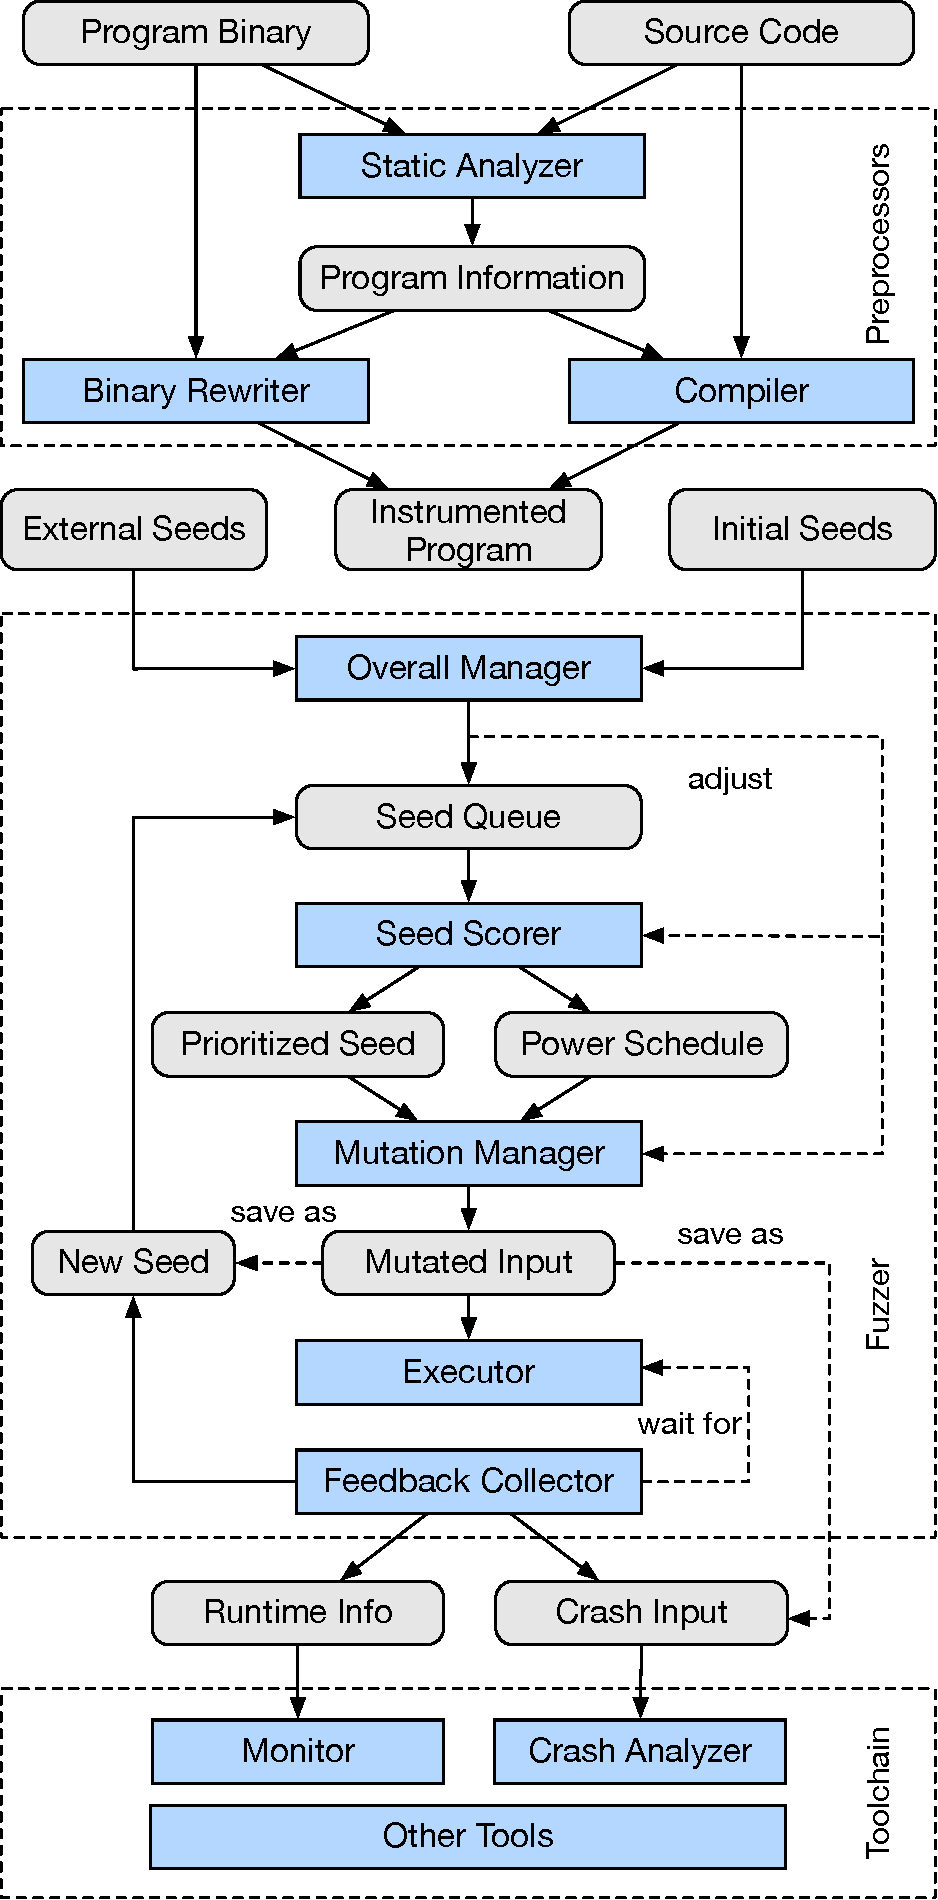
\includegraphics[width=0.64\textwidth]{res/fot/FOT_overview}
	\caption{Overview of the {\FOT} Fuzzing Framework}
	\label{fig:fot_workflow}
\end{figure}

Fig.~\ref{fig:fot_workflow} depicts the overview of {\FOT}.
It has three parts (labeled in pink): the \emph{preprocessor}, the \emph{fuzzer}, and the \emph{complementary toolchains}.
Components of the framework are represented with \emph{blue} rectangles while the inputs and outputs are in \emph{grey}. All these components inside \FOT are \textit{configurable} and \textit{extensible}.


\subsection{Preprocessor}
This contains various tools to collect static information and apply instrumentations.


\subsubsection{Static Analyzer}\label{sec:static_analysis}
It consists of tools to extract semantics from the PUT.
For example, we provide tools to generate the control flow graph, call graph or statically predicted vulnerabilities and convert them into proper representations which can be later instrumented into the PUT and utilized during dynamic fuzzing.
It is \textit{configurable} to generate different levels of static information. It is \textit{extensible} as developers are allowed to add new types of static analysis as long as the generated result follows the specified format.


\subsubsection{Instrumentor}
\emph{Binary rewriter} and \emph{source transformer} instrument static results generated by the static analyzer into the PUT for the fuzzer to collect feedback during runtime execution.
{\FOT} supports LLVM based instrumentation when program source is available, and Dyninst~\cite{dyninst} instrumentation when only the binary is given.
It is \textit{configurable} since the users can choose to instrument either on source code or binary.
It is \textit{extensible} since developers can use instrumentors such as Intel PIN~\cite{pin} as long as the instrumented code can embed the static information and provide sufficient feedback during fuzzing.

\subsection{Fuzzer}
This part explains the core fuzzing process. 
The fuzzer is essentially a loop that continuously selects seeds from a seed queue, applies mutations to the selected seeds, executes the PUT against mutated inputs, and collects statistics for the next iteration.

\subsubsection{Conductor}
As {\FOT} is designed to support multi-threaded parallel fuzzing, it contains the \emph{conductor} for fuzzing, scheduling the workload of different fuzzing instances.
Particularly, it monitor a special directory to actively import seed inputs from external tools such as symbolic executors (e.g., KLEE~\cite{klee}) or mutation generators (e.g., Radamsa~\cite{radamsa}).
It is \textit{configurable} since the users are allowed to choose different strategies for the overall management.
It is \textit{extensible} since it can interoperate with other external tools.


\subsubsection{Seed Scorer}
The seed scorer is in charge of selecting a seed from the queue for mutation (seed selection/prioritization) and determining how many new inputs should be generated based on the selected seed (power scheduling).
It is \textit{configurable} since the users can select from several built-in scoring strategies to evaluate seeds.
It is \textit{extensible} since the developers can implement their own strategies with the provided interfaces.


\subsubsection{Mutation Manager}
The mutation manager schedules different kinds of mutators.
It is \textit{configurable} as {\FOT} provides various mutators the their combinations for the users to select from.
It is \textit{extensible} as the developers can implement their own mutators with the provided interfaces.

\subsubsection{Executor}
The executor drives the execution of the PUT.
It is \textit{configurable} since the default executor in {\FOT} allows users to choose whether or not to use forkserver~\cite{afl} during fuzzing.
It is \textit{extensible} since the developers can extend the executor for various scenarios.
For example, they may add a secondary executor to execute another PUT for differential testing.

\subsubsection{Feedback Collector}
The feedback collector collects the feedback emitted by the PUT.
The exact feedback often corresponds to the instrumented information.
It is \textit{configurable} as the users are allowed to select from the default feedback options provided by {\FOT}.
For now, the feedback can be at basic-block level (like {\AFL}) or function level.
It is \textit{extensible} as the users can specify their customized types of feedback for collection.

\subsection{Complementary Toolchain}
{\FOT} contains various tools helping to make the framework \textit{versatile}.
For instance, we implemented a web-based frontend user interface to monitor the overall results.
It provides fruitful information to make the fuzzing process more transparent.
We also provided a crash analyzer to analyze the detected crashes and automatically generate reports.
This greatly reduces the manual efforts of crash triaging.
Many other extensions are also being added to complement the fuzzer.


\begin{figure}[t]
	\centering
	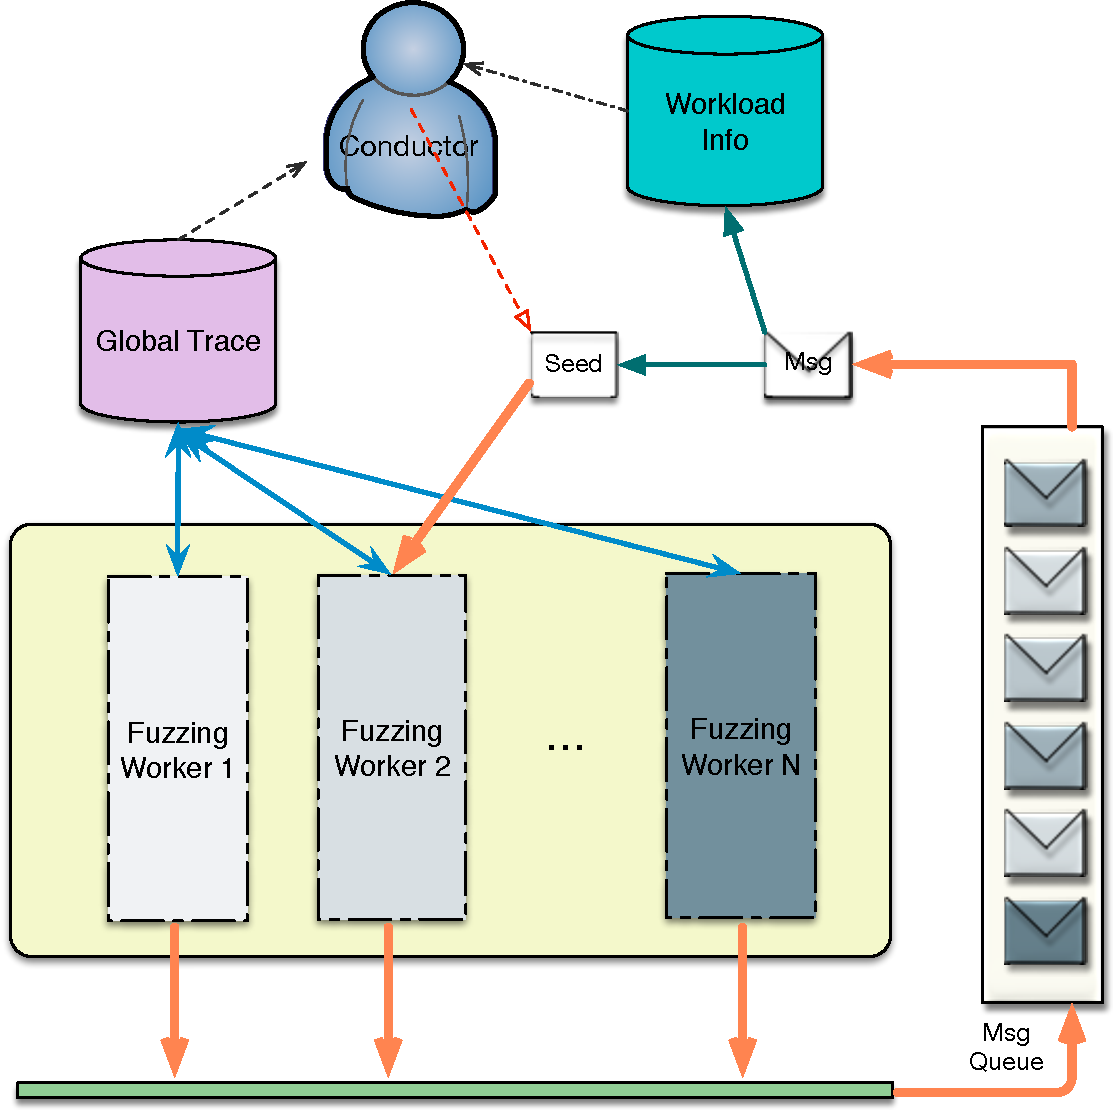
\includegraphics[width=0.6\columnwidth]{res/fot/mt_workflow}
	\caption{Coordination among Different Fuzzing Instances}
	\label{fig:mt_workflow}
\end{figure}


\subsection{Trace Update and Synchronization}\label{sec:trace_sync}
One of {\FOT}'s key features is the builtin coordination among different fuzzing instances (Fig.~\ref{fig:mt_workflow}). One important issue is the trace synchronization between fuzzing instances. For instrumentation, we made a slight change to the conventional instrumentation runtime to make the target binaries able to distinguish different shared memory arenas and the file descriptors used for ``forkserver'' allocated/specified by different fuzzing workers. Each fuzzing worker allocates the shared memory and the instrumented binary writes to specific multiple 8-byte areas when the corresponding ``execution edges'' have been reached. By auditing the byte fingerprints, the fuzzer knows about the edges and their approximate hit counts within this run. This information sits between between ``branch coverage'' and ``path coverage''. By comparing the shared memory fingerprint with the local trace information (checking whether the active shared memory byte has been marked ``traced'' locally), the fuzzer gets the knowledge whether current running seed increases the coverage. Updating of the local trace is majorly a ``bitwise and'' where each byte of the local trace is initialized with all ones (i.e., 255).

The local trace is synchronized with the global trace state. There stands a tradeoff: if we use directly the global trace state, the synchronization will be too frequent and eventually decreases performance with the increase of more fuzzing workers; if the fuzzers are only aware of the local trace, it is no better than {\AFL}'s na\"ive approach that runs all instances separately. We thus choose to only apply the synchronization during the mutation of each test case in the queue, when customizable conditions are triggered (usually the conditions are about the executions and time since last synchronization).

The actual synchronization of the trace information still applies ``bitwise and'' on normal running traces from local trace information to global state, and an instant copy in the other direction. This is far more efficient than {\AFL}'s synchronization by 1) importing seeds from other directories and 2) running all the test cases indistinguishably. Note that {\FOT}'s synchronization does not lose precisions compared to {\AFL}'s, where both ``bitwise and'' operations erase the exact hit count information.


  \subsection{Mutation Strategy Adaption}\label{sec:mutation_ops}
 The selection of mutation operators during fuzzing on one test input is determined by two factors:
 \begin{enumerate}
 	\item The whitelist mutation operators used for the targeted binaries. Some mutation operators are only effective on certain programs, but is almost a waste of time for the other programs (for example, bitflip operations are quite expensive and rarely useful for text-based parser programs running against large files). This can be specified by the experienced {\FOT} users.
 	\item The one-time mutation operators for \emph{this fuzz}. This is automatically determined by the fuzzer according to statistics generated from the previous mutations and runs. It is calculated in an adaptive way and may finally help to determine the ``convergence'' of the test cases.
 \end{enumerate}

On the other hand, being super general, {\AFL} has limited configurations for what mutation operators can be used and frequently runs blindly on the mutations that do not fit well~\cite{junjie:2017sp:skyfire,mopt-fuzz}.


\subsection{Refinement on Variable Behaviors}\label{sec:entry_var_behavior}

Some programs have variable behaviors for the same input test, due to randomness, multi-threading, etc. {\AFL} handles this issue by running all the newly found interesting test cases multiple times (known as \emph{calibration}); whenever it finds that the shared memory information (the active bytes and their hit count) differs from the first run, it will give more chances to the running test entry, and then keeps track of the variable behavior rate. The problem is that it does not utilize the information further since variable behaviors may cause certain runs to exit normally at some time, however crash at other time, which is more serious. We separately track those test case and give even more chances for these seeds. Alternatively, we provide an intrinsic strategy to prioritize these cases and let those test cases to be more likely to run next time. On the other hand, {\AFL}'s tracing information for the variable behavior cases are imprecise since it only traces the last calibration shared memory; we refine this by (selective) ``bitwise or'' operations to the shared memory for subsequent procedures on the current seed.


 \subsection{Trimming on Duplicated Cases}
Due to the existence of the potential lag of the trace synchronization, there still exists test input that runs with the same running trace. In other cases, the test cases might not be in its ``simplest'' form: by removing some bytes, the input test case can still results in the same running trace. {\FOT}'s approach in handling this is to trim the calibrated test cases immediately before being parceled as the message and sent to the message queue buffer managed by the conductor. And the conductor maintains a checksum set of all the generated seed files. Therefore when the newly generated seed has the same checksum as one of the existing ones, this test case will be discarded.

Additionally, we provide an external minimizer program to prune the all the serialized test cases (which can be normal runs, timeout runs, or crashes); it is more aggressive than the embedded procedure in the fuzzer and aims to provide a minimized version of all the interesting test cases.
 

\subsection{Implementation}\label{sec:fot-impl}

The {\FOT} project started from June, 2017 and has been actively developed by two researchers. It is implemented with 16000 lines of Rust for core fuzzing modules, together with 4500 lines of C/C++ for the preprocessor, 4200 lines of Java for structure-aware mutation, and 2400 lines of Python for complementary toolchain.
  

\section{Comparisons to Other Fuzzing Frameworks and Extensions}


In this section, we first compare FOT with other fuzzing frameworks, and then discuss its relationship to current fuzzing extensions.



Table~\ref{tbl:cmp_fuzz} compares {\FOT} with existing fuzzing frameworks with respect to 10 major features. As we can see, the existing fuzzing frameworks AFL, libFuzzer and honggfuzz lack \FOT's features in various aspects. {\FOT} stands out in that it provides multiple configurations for advanced users; it is also highly modularized, suitable to be extended with other fuzzing techniques. Moreover, {\FOT} partially supports structure-aware mutations and interoperability with other external tools such as symbolic executors (by monitoring and scheduling newly incoming seed input directory).

Most current fuzzing extensions can be easily integrated into {\FOT} owing to its design. In reality, they can be applied with some extensions to the different components in Figure~\ref{fig:fot_workflow} and can be used together with the configuration interface. 

\begin{enumerate}[1)]
	\item AFLFast~\cite{Bohme:2016:CGF} can be implemented by applying a Markov Chain model based seed \emph{power scheduling} in the fuzzer. 
	\item AFLGo~\cite{Bohme:2017:DGF} can be implemented by a combination of \emph{static analyzer}, \emph{instrumentation} and \emph{power scheduling}.
	\item CollAFL~\cite{CollAFL} can be implemented by using a collision-resistant algorithm to increase the uniqueness of the path trace labeling during \emph{instrumentation}.
	\item Skyfire~\cite{junjie:2017sp:skyfire}, Radamsa~\cite{radamsa}, Csmith~\cite{csmith} can be used in the preprocessor to generate seeds for the \emph{external seeds} and a structure-aware mutator assigned by \emph{mutation manager}.
	\item Symbolic executors such as KLEE~\cite{klee} can be integrated in the Driller's~\cite{driller} style with the help of \emph{conductor}.
\end{enumerate}

\begin{table}[t]
\centering
	\small
	\caption{Comparisons between fuzzing frameworks (\Circle: not supported, \LEFTcircle: partially supported, \CIRCLE: fully supported)}
	\label{tbl:cmp_fuzz}
	\begin{tabular}{|l|c|c|c|c|}
		\hline
		\diagbox{\textbf{Features}}{\textbf{Framework}} & \textbf{AFL} & \textbf{libFuzzer} & \textbf{honggfuzz} & \textbf{FOT} \\ \hline\hline
		Binary-Fuzzing Support & \CIRCLE & \Circle & \CIRCLE & \CIRCLE \\ \hline
		Multi-threading Mode & \Circle & \CIRCLE  & \CIRCLE  & \CIRCLE  \\ \hline
		In-memory Fuzzing &\CIRCLE  & \CIRCLE &\CIRCLE  & \CIRCLE \\ \hline
		Advanced Configuration & \Circle  & \LEFTcircle  & \Circle  & \CIRCLE  \\ \hline
		Modularized Functionality & \Circle & \LEFTcircle & \Circle & \CIRCLE \\ \hline
		Structure-aware Mutation & \Circle  &\Circle & \Circle  & \LEFTcircle \\ \hline
		Interoperability & \Circle & \Circle & \Circle & \LEFTcircle \\
		\hline
		Toolchain Support &  \CIRCLE & \Circle  & \Circle  & \CIRCLE \\ \hline
		Precise Crash Analysis & \Circle  & \Circle  & \CIRCLE  & \CIRCLE  \\ \hline
		Runtime Visualization & \LEFTcircle & \Circle & \Circle & \CIRCLE \\ \hline
	\end{tabular}
\end{table}


\subsection{New Vulnerabilities}

At the time of writing, {\FOT} has been used to fuzz more than 100 widely used open source projects and it has detected more than 200 vulnerabilities, among these 51 CVE IDs have been assigned. The detailed information is available at Appendix~\ref{app:bugs}. Notably, \FOT has detected multiple vulnerabilities with \emph{high} or \emph{critical} severity. For example, CVE-2019-9169~\cite{CVE-2019-9169} stresses a vulnerability in the GNU C Library (a.k.a glibc or libc6 on Linux distributions) through 2.29, where the function \func{proceed\_next\_node} inside POSIX regular expression (regex) component has a heap-based buffer over-read via an attempted case-insensitive regex match. Thanks to the interoperability with the regex generators, FOT is able to generate more meaningful seeds that cover more corner cases of the regex components. According to CVSS v3.0 Severity and Metrics~\cite{cvss3}, it is scored 9.8 out of 10.0 (critical severity); according to CVSS v2.0~\cite{cvss2}, it has a score of 7.5 (high severity). As a comparison, the notorious HeartBleed (CVE-2014-0160) is scored 5.0 medium severity according to CVSS v2.0 (there is no CVSS v3.0 for it). Many of other vulnerabilities discovered by \FOT also have high severity, e.g, CVE-2018-15822, CVE-2018-14394, CVE-2018-14395 in FFmpeg, CVE-2018-19837, CVE-2018-19838, CVE-2018-19839, CVE-2018-20821, CVE-2018-20822 in libsass, CVE-2018-14560, CVE-2018-14561, CVE-2019-11470, CVE-2019-11472 in ImageMagick, and CVE-2019-11473, CVE-2019-11474 in GraphicsMagick. We envision that with more integrated fuzzing techniques, \FOT will have the capabilities to detect more vulnerabilities that are hard to be discovered by existing fuzzers.


\fancyhead[RE,LO]{\fancyplain{}{\leftmark}}
\renewcommand{\chaptermark}[1]{\markboth{\chaptername\ \thechapter.\ \emph{Security Type Checking for Android Access Control}}{}}
% !TeX root =../../main.tex

\chapter{Type Checking Based Verification} \label{ch:sta}

\section{Introduction and Motivation}\label{sec:sta_intro}

Owing to the pervasive use of mobile applications (apps), mobile security has become increasingly important for our daily life.
Among all different kinds of mobile devices, Android accounts for the majority of them. Due to this, security analysis on them has been of significant interests. There has been a quantity of analyses on Android security~(\cite{Enck:2009:UAS:1512148.1512324, Fuchs2010, Arzt:2014:FPC:2666356.2594299, Wei:2014:APG:2660267.2660357, Li:2015:IDI:2818754.2818791}) that focus on detecting potential security violations. Here we are interested in the problem of constructing secure apps.
In particular, we aim to provide a guarantee for information flow security in the constructed apps. In order to achieve this, we apply a type checking based verification approach.

\subsection{Motivating Examples}


During designing an information flow type system for Android, we encounter
a common pattern of conditionals that would not be typeable using conventional type systems.
Consider the pseudo-code in Listing~\ref{lst:eg_contact}.
\begin{figure}[ht]
\begin{lstlisting}[caption={Sample code for getting contact info with a permission check.}, label={lst:eg_contact}]
String getContactNo(String name) {
    String number;
    if(checkPermission(READ_CONTACT))
       number = ... ;
    else number = "";
    ret number;
}
\end{lstlisting}
\end{figure}
Such a code fragment could be part of a phone dialer or a social network service app such as Facebook, WhatsApp, where \textit{getContactNo} provides
a public interface to query the phone number associated with a name. The (implicit) security policy in this
context is that contact information (the phone number) can only be released if the calling app has
READ\_CONTACT permission.
The latter is enforced using the \textit{checkPermission} API in Android.
Suppose phone numbers are labelled with $H$, and the empty string is labelled with $L$.
If the interface is invoked by an app that has the required permission,
the phone number ($H$) is returned; otherwise an empty string ($L$)
is returned. In both cases, no data leakage happens: in the former case, the calling app is authorized; and in the latter case, no sensitive data is ever returned. By this informal reasoning, the function complies with the implicit security policy and it
should be safe to be called in \emph{any} context, regardless of the permissions the calling app has.
However, in the traditional (non-value dependent) typing rule for the if-then-else construct, one would assign \emph{the same} security labels to both branches,
and the return value of the function would be assigned level $H$.
As a result, if this function is called from an app with \emph{no} permission, assigning the return value to a variable with security labels $L$ has to be rejected by the type system even though no sensitive information is leaked.
To cater for such a scenario, we need to make the security type of \textit{getContactNo}
 \emph{depend on} the permissions possessed by the caller.

Banerjee and Naumann~\cite{Banerjee:2005ht} proposed a type system (refered to as {\BN} system)
that incorporates permissions into function types.
Their type system was designed for an access control mechanism different from ours,
but the basic principles are still applicable.
In {\BN} system, a Java class may be assigned a set of permissions which need to be {\em explicitly enabled} via an \textbf{enable} command for them to have any effect.
We say a permission is {\em disabled} for an class if it is \emph{not assigned} to the class, or it is \emph{assigned} to the class but is \emph{not explicitly enabled}.
Depending on the permissions of
the calling class (corresponding to an \emph{app} in the above example), a function such as \textit{getContactNo} can have a collection of types. In {\BN} system, the types of a function take
the form $(l_1,\dots, l_n)\xrightarrow{~P~}l$
where $l_1,\dots,l_n$ denote security labels of the input, $l$ denotes the security labels of the output
and $P$ denotes a set of permissions that are disabled by the caller.
The idea is that permissions are guards to sensitive values. Thus conservatively, one would type the return value of \textit{getContactNo} as $L$ only if
one knows that the permission READ\_CONTACT is disabled.
In {\BN} system, \textit{getContactNo} admits:% the following types:
{\myeqsize\begin{equation*}
\textit{getContactNo} : L~\xrightarrow{~P~}~L\qquad
\textit{getContactNo} : L~\xrightarrow{~\emptyset~}~H
\end{equation*}}
where $P = \{ \mathrm{READ\_CONTACT} \}.$
When typing a call to \textit{getContactNo} by
an app without permissions,
the first type of \textit{getContactNo} is used; otherwise
the second type.% is used.

In {\BN} system, the typing judgment is parameterized
by a permission set $Q$ containing the permissions that are
currently known to be disabled. The set $Q$ may or may not contain all disabled permissions.
Their language features a command ``\lcCP{P}{c_1}{c_2}'', which
means that if the permissions in the set $P$ are \emph{all enabled}, then
the command behaves like $c_1$; otherwise it behaves like $c_2$.
The typing rules for the \textit{test} command (in a much
simplified form) are:
{\myeqsize\[
\inference[(R1)~]{
Q \cap P = \emptyset & Q |- c_1 : t & Q \vdash {c_2} : t
}
{
Q \vdash \lcCP{P}{c_1}{c_2} : t
}
\]
\[
\inference[(R2)~]{
Q \cap P \not = \emptyset & Q \vdash c_2 : t
}
{
Q \vdash \lcCP{P}{c_1}{c_2} : t
}
\]}
where $Q$ is a set of permissions that are disabled.
When $Q \cap P \not = \emptyset$, then
at least one of the permissions in $P$ is disabled, thus
one can determine statically that ``\textbf{test}(P)'' would fail and only the \emph{else} branch would be executed at runtime. This case is
reflected in the typing rule R2.
When $Q \cap P = \emptyset$, there can be two possible runtime scenarios.
One scenario is that all permissions in $P$ are enabled, so ``\textbf{test}(P)'' succeeds and $c_1$ is executed.
The other is that some permissions in $P$ are disabled, but are not accounted for in $Q$.
So in this case, one cannot determine statically which branch of \textbf{test} will be
taken at runtime. Therefore, R1 conservatively considers typing both branches.

When adapting {\BN} system to Android, R1
is still too strong in some scenarios, especially when it is desired that the \emph{absence} of some permissions
leads to the release of sensitive values. Consider for example an application
that provides location tracking information related to a certain
{\em advertising ID} (Listing~\ref{lst:eg_nonmonotonic}), where the latter provides a unique ID for the purpose of anonymizing mobile users
to be used for advertising (instead of relying on hardware device IDs such
as IMEI numbers). If one can correlate an advertising
ID with a unique hardware ID, it will defeat the purpose of
the anonymizing service provided by the advertising ID. To prevent
that, \textit{getInfo} returns the location information for an advertising ID
only if the caller \emph{does not} have access to device ID.
To simplify discussion, let us assume that the permissions to access
IMEI and location information are denoted by $p$ and $q$, respectively.
\begin{figure}[ht]
\begin{lstlisting}[caption={An example about non-monotonic policy.}, label={lst:eg_nonmonotonic}]
String getInfo() {
   String r = "";
   test(p) {
     test(q) r = loc; else r = "";
   } else  {
     test(q) r = id++loc; else r = "";
   }
   ret r;
}
\end{lstlisting}
\end{figure}
Here \textit{id} denotes a unique advertising ID  generated and stored by the app for
the purpose of anonymizing user tracking and \textit{loc} denotes location
information.
The function first tests whether the caller has access to IMEI number.
If it does, and if it has access to location, then only the location information is returned.
If the caller has no access to IMEI number, but can access location information,
then the combination of advertising id and location \textit{id++loc} is returned.
In all the other cases, an empty string is returned.
Let us consider a lattice with four elements ordered as:
$L \leq l_1, l_2 \leq H$, where $l_1$ and $l_2$ are incomparable. We specify that empty string is of type $L$, \textit{loc} is of type $l_1$,
\textit{id} is of type $l_2$, and the aggregate \textit{id++loc} is of type $H.$
Consider the case where the caller has permissions $p$ and $q$ and both are (explicitly) \emph{enabled}.
When applying {\BN} system, the desired type of \textit{getInfo} in this case is  $()~{\xrightarrow{~\emptyset~}}~l_1$.
This means that the type of \textit{r} has to be at most $l_1$.
Since no permissions are disabled, only \ruleTagText{R1} is applicable
to type this program. This, however, will force both branches of \textbf{test}(p)
to have the same type. As a result, \textit{r}
has to be typed as $H$ so that all four assignments in the program
can be typed.

The issue with the example in Listing~\ref{lst:eg_nonmonotonic} is that the stated security policy is \emph{non-monotonic} in the sense that an app with more permissions does not necessarily have access to information with higher
level of security.  The fact that {\BN} system
cannot precisely capture non-monotonic policies appears to be a design decision:
they cited in \cite{Banerjee:2005ht} the lack of motivating examples for non-monotonic policies, and
suggested that to accommodate such policies one might need to consider a notion of declassification.
As we have seen, however, non-monotonic policies can arise naturally in mobile
apps. In a study on Android
malwares~\cite{Enck:2009:UAS:1512148.1512324}, Enck et. al. 
identify several combinations of permissions that are potentially
`dangerous', in the sense that they allow potentially unsafe information flow.
An information flow policy that requires
the {\em absence} of such combinations of permissions in 
information release would obviously be non-monotonic.
In general, non-monotonic policies can be required to solve the {\em aggregation problem}
studied in the information flow theory~\cite{Landauer93}, where several pieces of low security labels information may
be pooled together to learn information at a higher security labels.

We therefore designed a more precise type system for information flow
under an access control model inspired by Android framework.
Our type system solves the problem of typing non-monotonic policies
without resorting to downgrading or declassifying information.
It is done technically via a \emph{merging} operator on security types, to keep information related to both
branches of \textbf{test}. Additionally, there is a significant
difference in the permission model used in traditional type systems such as {\BN} system, where permissions
are propagated across method invocations among apps. This is due to the fact that permissions in Android are relevant only during inter-process calls, while permissions are not inherited along the call
chains across apps. As we shall see in ~\S\ref{sec:typing_rules}, this may give rise to a type of attack which we call
``parameter laundering'' attack if one adopts a naive typing rule for function calls.
The soundness proof for our type system is significantly different from that for {\BN} type system due to the difference
in permission model and the new merging operator on types in our type system.

\subsection{Contributions}
The contributions of this chapter are threefold.
\begin{enumerate}\item We develop a lightweight type system where security types are dependent on a permission-based access control mechanism, and prove its soundness in terms of non-interference (\S\ref{sec:type_system}). A novel feature of our type system is the type merging constructor, used for typing the conditional branch for permission checking. This makes it possible to model non-monotonic information flow policies.
	\item We identify a problem of explicit flow through function calls in the setting where permissions are not propagated during calls. This problem
	arises as a byproduct of Android's permission model, which is significantly different from that in JVM, and adopting a standard typing rule for function calls such as the one proposed for Java in~\cite{Banerjee:2005ht} 
	would result in unsoundness. We name this the parameter laundering problem and propose a typing rule for function calls that prevents it.
	\item We provide a type inference for our proposed type system, and show its decidability by reducing it to a constraint solving problem (\S\ref{sec:constraint_gen}).
\end{enumerate}
 \section{A Secure Information Flow Type System}\label{sec:type_system}

In this section, we present the proposed information flow type system. \S\ref{sec:permission_model} discusses informally a permission-based access control model, which is an abstraction of the permission mechanism used in Android.
 \S\ref{sec:language} and ~\S\ref{sec:semantics} give the operational semantics of a simple imperative language that includes permission checking
constructs based on the abstract permission model.
~\S\ref{sec:types} and ~\S\ref{sec:typing_rules} describe our type system and prove its soundness in terms of non-interference.

\subsection{A Model of Permission-based Access Control}
\label{sec:permission_model}

Instead of taking all the language features and the library dependencies of Android apps into account, we focus on the permission model used in inter-component communications within and across apps. Such permissions are used to regulate access to protected resources, such as device id, location information, contact information, etc.

In Android, an app specifies its required permissions at installation time via a manifest file. In recent versions of Android (since Android 6.0, API level 23), some of these permissions need to be granted by users at runtime. But
at no point a permission request is allowed if it is not already specified in the manifest.
For now, we assume a permission enforcement mechanism that applies to Android versions prior to version 6.0, so it does not
account for permission granting at runtime. To be specific, runtime permission request requires the compatible version specified in the manifest file to be greater than or equal to API level 23, and the running OS should be at least Android 6.0~\cite{url:android-perm}. Runtime permission granting poses some problems in typing non-monotonic policies, which shall be discussed further in ~\S\ref{sec:conclusion}.

An Android app may provide services to other apps,
or other components within the app itself. Such a service provider
may impose permissions on other apps who want to
access its services. Communication between apps is implemented
through Binder IPC (inter-process communications)~\cite{Android-Binder-IPC}.

In our model, a program is an abstracted version of an app, and the intention is to show how one can reason about information flow in such a service provider when access control is imposed on the calling app. In the following we will not model explicitly the IPC mechanism of Android, but instead model it as a function call. Note that this abstraction is practical since it can be achieved by conventional data and control flow analyses, with the extra modeling of Android IPC specific APIs. The feasibility has been demonstrated by frameworks like FlowDroid~\cite{Arzt:2014:FPC:2666356.2594299}, Amandroid~\cite{Wei:2014:APG:2660267.2660357}%
%~\footnote{We have also been implementing a permission-dependent information flow analysis tool on top of Amandroid. The basic idea is similar to the one mentioned in this chapter, however the focus is improving the precision of information leakage detection rather than non-interference certification.}
, IccTA\cite{Li:2015:IDI:2818754.2818791}, etc.

One significant issue that has to be taken into account is that Android framework does not track IPC call chains between apps and permissions of an app are not propagated to the callee. That is, an app $A$ calling another app $B$ does not grant $B$ the permissions which have been assigned to $A$. This is different from the traditional type systems such as {\BN} where permissions can potentially propagate along the call stacks. Note however that $B$ can potentially have more permissions than $A$, leading to a potential privilege escalation, a known weakness in Android permission system~\cite{Chin:2011wa}. Another consequence of lacking transitivity is that in designing the type system, one must take care to avoid what we call a ``parameter laundering" attack (c.f. ~\S\ref{sec:types}).

\subsection{A Language with Permission Checks}\label{sec:language}

As mentioned earlier, we do not model directly all the language features of an Android app, but use a much simplified language to focus on the permission mechanism part. The language is a variant of the  language considered in \cite{Volpano:1996}, extended with functions and an operator for permission checks.

We model an \emph{app} as a collection of \emph{functions}
(\emph{services}), together with a statically assigned permission
set. A \emph{system}, denoted by $\mathcal{S}$, consists of a set of
apps. We use capital letters $A,B,\ldots$ to denote apps. A function
$f$ defined in an app $A$ is denoted by $A.f$, and may be called
independently of other functions in the same app. The intention is
that a function models an  application component (i.e.,
\emph{Activity}, \emph{Service}, \emph{BroadCastReceiver}, and
\emph{ContentProvider}) in Android, which may be called from within
the same app or other apps.

We assume that only one function is
executed at a time, so we do not model concurrent executions of
apps. We think that in the Android setting, considering sequential behavior only is
not overly restrictive. This is because the communication between apps are
(mostly) done via IPC. Shared states between apps,
which is what contributes to the difficulty in concurrency handling, is mostly
absent, apart from the very limited sharing of preferences. In such a setting,
each invocation of a service can be treated independently as there is usually
no synchronization needed between different invocations. Additionally, we assume functions in a system are not (mutually)
recursive, so there is a finite chain of function calls from any given
function. The absence of recursion is not a restriction, since our
functions are supposed to model communications in Android, which are
rarely recursive. We denote with $\PS$ the finite set containing all permissions in
the system. Each app is assigned a static set of permissions drawn
from this set. The powerset of $\PS$ is written as~$\PPS$.  


For simplicity, we consider only programs manipulating \emph{integers}, so the expressions in our language all have the integer type. Boolean values are encoded as 0 (false) and any non-zero values (true). The grammar for expressions is given below:
{\myeqsize\begin{equation*}
e ::= n \mid \leVAR{x} \mid \leOP{e}{e}
\end{equation*}}
where $n$ denotes an integer literal, $\leVAR{x}$ denotes a variable, and $\leOP{}{}$ denotes a binary operation.
The commands of the language are given in the following grammar:
{\myeqsize\begin{equation*}
\begin{array}{l}
  c\;::=\; \lcASS{x}{e} \mid \lcIF{e}{c}{c} \mid  \lcWHILE{e}{c} \mid \lcSEQ{c}{c}  \\
  \quad \mid \lcLETV{x}{e}{c} \mid \lcCALL{x}{A.f}{\overline{e}} \mid \lcCP{p}{c}{c}
\end{array}
\end{equation*}}
The first four constructs are assignment, conditional, while-loop and sequential composition, respectively.
The statement ``\lcLETV{x}{e}{c}'' is a local variable declaration statement. Here $x$ is
declared and initialized to $e$, and its scope is the command $c$. We require
that $x$ does not occur in $e.$
The statement ``\lcCALL{x}{A.f}{\overline{e}}''  denotes an assignment whose right hand side is
a function call to $A.f$. The statement
``\lcCP{p}{c_1}{c_2}''
checks whether the calling app has permission $p$: if so then $c_1$ is executed,
otherwise $c_2$ is executed.
This is similar to the \textbf{test} construct in {\BN} system, except that we allow testing only
one permission at a time. This is a not real restriction since both versions of the \textbf{test} can simulate one another.


A function declaration has the following syntax:
{\myeqsize\begin{equation*}
F ::= \lpPROG{A.f}{\overline{x}}{c}{{\lpRES}}
\end{equation*}}
where $A.f$ is the function name, $\bar x$ are function parameters,
$c$ is a command, and {\lpRES} is a local variable
that holds the return value of the function.
$\overline{x}$ and $r$ are bound variables with the command ``$c; \textbf{ret}~r$'' in their scopes.
We consider only {\em closed functions}, i.e., the variables occurring in $c$
are either introduced by \textbf{letv} or from the set $\{\overline{x}, r\}$.



\begin{figure*}[ht]
{\tiny
\[
\inference[E-VAL]{}{\mu \vdash \leVAL{v}  \leadsto v}
\qquad
\inference[E-VAR]{}{\mu \vdash \leVAR{x}  \leadsto \mu(x)}
\]

\[
\inference[E-OP]{\mu \vdash e_1 \leadsto v_1\quad \mu \vdash e_2 \leadsto v_2}
{\mu \vdash \leOP{e_1}{e_2} \leadsto \leOP{v_1}{v_2}}
\qquad
\inference[E-LETV]{\mu \vdash e \leadsto v \quad \mu [ x \mapsto v ]; A ; P \vdash c \leadsto \mu'}
{\mu; A; P \vdash \lcLETV{x}{e}{c} \leadsto \mu' - x}
\]

\[
\inference[E-SEQ]{\mu;A; P \vdash c_1 \leadsto \mu' \quad \mu';A; P \vdash c_2 \leadsto \mu''}
{\mu;A;P \vdash \lcSEQ{c_1}{c_2} \leadsto \mu''}
\qquad
\inference[E-ASS]{\mu \vdash e \leadsto v}
{\mu; A; P \vdash \lcASS{x}{e} \leadsto \mu [ x \mapsto v ]}
\]

\[
\inference[E-IF-T]{\mu \vdash e \leadsto v\quad v\neq 0\quad \mu; A; P \vdash c_1 \leadsto \mu'}
{\mu; A; P \vdash \lcIF{e}{c_1}{c_2} \leadsto \mu'}
\qquad
\inference[E-IF-F]{\mu \vdash e \leadsto v\quad v = 0\quad \mu;A; P \vdash c_2 \leadsto \mu'}
{\mu;A; P \vdash \lcIF{e}{c_1}{c_2} \leadsto \mu'}
\]

\[
\inference[E-WHILE-T]{
\mu \vdash e \leadsto v\quad v\neq 0\quad
\mu;A; P \vdash c \leadsto \mu'\\
\quad \mu' ; A ; P \vdash \lcWHILE{e}{c} \leadsto \mu''
}
{\mu;A; P \vdash \lcWHILE{e}{c} \leadsto \mu''}
\qquad
\inference[E-WHILE-F]{\mu \vdash e \leadsto v\qquad v = 0}
{\mu;A; P \vdash \lcWHILE{e}{c} \leadsto \mu}
\]

\[
\inference[E-CP-T]{p\in P \quad \mu; A; P \vdash c_1 \leadsto \mu'}
{\mu; A ; P \vdash \lcCP{p}{c_1}{c_2} \leadsto \mu'}
\qquad
\inference[E-CP-F]{p\notin P \quad \mu;A;P \vdash c_2 \leadsto \mu'}
{\mu;A;P \vdash \lcCP{p}{c_1}{c_2} \leadsto \mu'}
\]

\[
\inference[E-ICALL]{
\FD(B.f) = \lpPROG{B.f}{\overline{y}}{c}{\lpRES} \qquad
\mu\vdash\overline{e} \leadsto \overline{v} \quad
[\overline{y} \mapsto \overline{v}, r \mapsto 0] ; B; \Theta(A) \vdash c \leadsto \mu'}
{\mu;A;P \vdash \lcCALL{x}{B.f}{\overline{e}} \leadsto \mu[x \mapsto \mu'(r) ]}
\]
}
\caption{Evaluation rules for expressions and commands, in the presence of function definition table $\FD$ and permission assignment $\Theta.$
}
\label{fig:semantics}
\end{figure*}
 
\subsection{Operational Semantics}\label{sec:semantics}
We assume that function definitions are stored in a table $\FD$ indexed by function names, and the permission sets assigned to apps are given by a table $\Theta$ indexed by app names.

An {\termEmph{evaluation environment}
is a finite mapping from variables to values (i.e., integers in the simplified language).
We denote with $EEnv$ the set of evaluation environments.
Elements of $EEnv$ are ranged over by $\mu$.
We  use the notation
$[ x_1 \mapsto v_1, \cdots,  x_n \mapsto v_n]$
to denote an evaluation environment mapping variable $x_i$ to value $v_i$; this will sometimes be abbreviated as $[ \overline x \mapsto \overline v ].$
The domain of $\mu = [ x_1 \mapsto v_1, \cdots, x_n \mapsto v_n]$ (i.e., $\{x_1,\dots,x_n\}$) is denoted by $dom(\mu)$.
Given two environments $\mu_1$ and $\mu_2$, we define
$\mu_1\mu_2$ as the environment $\mu$ such that $\mu(x) = \mu_2(x)$ if $x \in dom(\mu_2)$,
otherwise $\mu(x) =\mu_1(x)$.
For example, $\mu[x \mapsto v]$ maps $x$ to $v$, and $y$ to $\mu(y)$
for any $y \in dom(\mu)$ such that $y \not = x.$
Given a mapping $\mu$ and a variable $x$, we write $\mu\!-\!x$ to denote the
mapping resulting from removing $x$ from $dom(\mu)$.

The operational semantics for expressions and commands is
given in Figure~\ref{fig:semantics}.
The evaluation judgment
for expressions has the form $\mu\vdash e\leadsto v$,
which states that expression $e$ evaluates to value $v$ when variables
in $e$ are interpreted in the evaluation environment $\mu.$
We write $\mu \vdash \overline{e} \leadsto \overline{v}$,
where $\overline{e}=e_1,\dots,e_n$ and $\overline{v} = v_1,\dots,v_n$ for some $n$,
to denote a sequence of judgments
$\mu \vdash e_1 \leadsto v_1, \ldots, \mu \vdash e_n \leadsto v_n.$

The evaluation judgment for commands takes the form
$\mu;A;P\vdash c \leadsto \mu'$
where $\mu$ is an evaluation environment before the execution
of the command $c$, and $\mu'$ is the evaluation environment
after the execution of $c$. Here $A$ refers to the app to which the command $c$ belongs.
The permission set $P$ denotes the {\em permission context}, i.e., it is the set of permissions of the app which invokes the function of $A$ in which the command $c$ resides. The caller
app may be $A$ itself (in which case the permission context will be the same as the permission set of $A$) but more often it is another app in the system.

The operational semantics of most commands are straightforward.
We explain the semantics of the \emph{test} primitive and the function call.
Rules (\ruleTagText{E-CP-T}) and (\ruleTagText{E-CP-F}) capture the semantics of the \textbf{test} primitive.
These are where the permission context $P$ in the evaluation judgement is used.
The semantics of function calls is given by (\ruleTagText{E-ICALL}). 
 Notice that $c$ inside the body of \emph{callee} is executed under
the permission context $\Theta(A)$, which is the permission set of $A$. The permission context $P$
in the conclusion of that rule, which denotes the permission of the app that calls $A$, 
is not used in the premise. That is, the permission context of $A$ is not inherited by 
the callee function $B.f$. This reflects the way permission contexts in Android
are passed on during IPCs~\cite{Android-CheckPerm,Android-Binder-IPC}, and is also a major difference
between our permission model and that in {\BN} type system,
where permission contexts are inherited by successive function calls.

 \subsection{Security Types}\label{sec:types}

In information flow type systems such as \cite{Volpano:1996}, it is common to adopt a lattice
structure to encode security labels. Security types in this setting are just security
levels. In our case, we generalize the security types to account for
the dependency of security labels on permissions. So we shall distinguish
security labels, given by a lattice structure which encodes sensitivity levels
of information, and security types, which are mappings from permissions to security labels.
We assume the security labels are given by a lattice $\SL$, with a partial order $\leq_{\SL}$.
Security types are defined in the following.

\begin{definition}\label{def:base_type}
A \termEmph{base security type} (or \termEmph{base type}) $t$ is a mapping from $\PPS$ to $\SL$.
We denote with $\Tcal$ the set of base types.
Given two base types $s$ and $t$, we say $s=t$ \text{iff} $s(P)=t(P)$ for all  $P\in\PPS$.
We define an ordering $\leq_\Tcal$ on base types as follows: 
$s\leq_\Tcal t$ \text{iff} $\forall$ $P\in \PPS$, $s(P) \leq_{\SL} t(P)$.
\end{definition}

\begin{lemma}\label{lem:tleq_po}
	$\leq_\Tcal$ is a partial order relation on $\Tcal$.
\end{lemma}
\begin{proof}
\begin{ProofEnumDesc}[style=standard]
	\item[\textbf{Reflectivity}] $\forall P, t(P)\leq_{\SL} t(P)$ therefore $t\leq_\Tcal t$.
	\item[\textbf{Antisymmetry}] $t\leq_\Tcal s\wedge s\leq_\Tcal t\iff \forall P, t(P)\leq_{\SL} s(P)
\wedge s(P) \leq_{\SL} t(P)$ therefore $\forall P, t(P)=s(P)$, which means that $s=t$.
	\item[\textbf{Transitivity}] if $r\leq_\Tcal s$ and $s\leq_\Tcal t$, $\forall P, r(P) \leq_{\SL} s(P)$ and $s(P)\leq_{\SL} t(P)$ therefore $r(P) \leq_{\SL} t(P)$, which means that $r \leq_\Tcal t$.
\end{ProofEnumDesc}
\end{proof}
As we shall see, if a variable is typed by a base type, the sensitivity of
its content may depend on the app's permissions which writes to the variable.
In contrast, in traditional information flow type systems,
a variable annotated with a security label has a fixed sensitivity level
regardless of the permissions of the app that writes to the variable.

The set of base types with the order $\leq_{\Tcal}$ forms a lattice. The join and meet
of the lattice are defined as follows:

\begin{definition}\label{def:type-cup-cap}
For $s, t\in\Tcal$, $s\sqcup t$ and $s\sqcap t$ are defined as
{\myeqsize\begin{align*}
(s\sqcup t)(P) =  s(P)\sqcup t(P), \forall P \in \PPS\\
(s\sqcap t)(P) =  s(P)\sqcap t(P), \forall P \in \PPS
\end{align*}}
\end{definition}


\begin{lemma}\label{lem:bound}
Given two base types $s$ and $t$, it follows that
\begin{enumerate}[label*=(\alph*)]
\item $s \leq_\Tcal s\sqcup t$ and $t\leq_\Tcal s\sqcup t$.
\item $s\sqcap t \leq_\Tcal s$ and $s\sqcap t \leq_\Tcal t$.
\end{enumerate}
\end{lemma}
 \begin{proof}
Immediately from Definition~\ref{def:base_type}.
 \end{proof}


\begin{lemma}\label{lem:lattice}
$(\Tcal, \leq_\Tcal)$ forms a lattice.
\end{lemma}
 \begin{proof}
 $\forall s,t\in\PPS$, according to Lemma~\ref{lem:bound}, $s \sqcup t$ is their upper bound. Suppose $r$ is another upper bound, i.e., $s\leq_\Tcal r$ and $t\leq_\Tcal r$, which means $\forall P\in\PPS, (s\sqcup t)(P)=s(P)\sqcup t(P)\leq_{\SL} r(P)$, so $s\sqcup t\leq r$. Therefore $s\sqcup t$ is the least upper bound of $\left\{s,t\right\}$. Similarly, $s\sqcap t$ is $s$ and $t$'s greatest lower bound. This makes $(\Tcal, \leq_\Tcal)$ a lattice.
 \end{proof}


From now on, we shall drop the subscripts in $\leq_{\SL}$ and $\leq_\Tcal$ when no ambiguity arises.



\begin{definition}
\label{def:embed}
Given a security label $l$, we define $\hat{l}$ as:
for all $P \in \PPS$, we have $\hat{l}(P) = l$.
\end{definition}

Accordingly, a security label $l$ can be lifted to the base type $\hat{l}$ that maps all permission sets to level $l$ itself.



 \begin{definition}\label{def:fun-type}
   A \termEmph{function type} has the form $\overline{t} \rightarrow t$, where $\overline{t}=(t_1,\ldots,t_m)$, $m\geq 0$ and $t, t_i$ are base types.
   The types $\overline t$ are the types for the arguments of the function and $t$ is the return type of the function.
 \end{definition}

\begin{lemma}\label{lem:promote-demote}
Given $P\in\PPS$ and $p\in\PS$,
%\leavevmode
\begin{enumerate}[label*={(\alph*)}]
  \item\label{lem:promote-demote-1} If $p \in P$, then $(t\uparrow_{p})(P) = t(P)$.
	\item\label{lem:promote-demote-2} If $p \notin P$, then $(t\downarrow_{p})(P) = t(P)$.
\end{enumerate}
\end{lemma}
 \begin{proof}
If $p\in P$, $P\cup\{p\}=P$, therefore $(t\uparrow_{p}) (P) = t(P\cup \{p\})=t(P)$; if $p\notin P$, $P\setminus\{p\}=P$, therefore $(t\downarrow_{p}) (P) = t(P\setminus\{p\})=t(P)$.
 \end{proof}

\begin{lemma}\label{lem:pd-order}
If $s\leq t$, then $s\uparrow_{p} \leq t\uparrow_{p}$ and $s\downarrow_{p} \leq t\downarrow_{p}$.
\end{lemma}
 \begin{proof}
For $P\in\PS$, since $s\leq t$, $s(P\cup\{p\})\leq t(P\cup\{p\})$ and $s(P\setminus\{p\})\leq t(P\setminus\{p\})$, according to Definition~\ref{def:base_type} and Definition~\ref{def:updown}, the conclusion follows.
 \end{proof}


In our type system, security types of  expressions (commands, functions, resp.) may be
altered depending on the execution context. That is, when an expression is used in
a context where a permission check has been performed (either successfully or unsuccessfully),
its type may be adjusted to take into account the \emph{presence} or \emph{absence}
of the checked permission.
Such an adjustment is called a {\termEmph{promotion} or a {\termEmph{demotion}.


\begin{definition}\label{def:updown}
Given a permission $p$, the \termEmph{promotion} and \termEmph{demotion} of a base type $t$
with respect to $p$ are: 
{\myeqsize\begin{align*}
(t\uparrow_{p}) (P) = t(P\cup \{p\}), \forall P\in \PPS
\tag{promotion}
\\
(t\downarrow_{p}) (P) = t(P\setminus\{p\}), \forall P\in \PPS
\tag{demotion}
\end{align*}}
The \termEmph{promotion} and \termEmph{demotion} of $\overline{t}\rightarrow t$,
where $\overline{t} = (t_1,\dots, t_m)$, are respectively:
{\myeqsize\begin{align*}
(\overline{t}\rightarrow t)\uparrow_{p} = \overline{t}\uparrow_{p} \rightarrow t\uparrow_{p},~
\text{where}~\overline{t}\uparrow_{p} = (t_1\uparrow_{p},\ldots, t_m\uparrow_{p}),
\\
(\overline{t}\rightarrow t)\downarrow_{p} = \overline{t}\downarrow_{p}\rightarrow t\downarrow_{p},~
\text{where}~\overline{t}\downarrow_{p} = (t_1\downarrow_{p},\ldots, t_m\downarrow_{p}).
\end{align*}}
\end{definition}








\subsection{Security Type System}\label{sec:typing_rules}


\begin{figure*}
\tiny
\[
\inference[T-VAR]{}
{\Psi \vdash \leVAR{x} : \Psi(x)}
\qquad
\inference[T-OP]
{\Psi\vdash e_1: t & \Psi ; A\vdash e_2: t}
{\Psi\vdash \leOP{e_1}{e_2} : t}
\qquad
\inference[T-SUB$_{e}$]
{\Psi\vdash e : s & s \leq t}
{\Psi\vdash e : t}
\qquad
\inference[T-SUB$_{c}$]
{\Psi; A \vdash c : s & t \leq s}
{\Psi; A\vdash c : t}
\]

\[
\inference[T-ASS]
{\Psi \vdash e : \Psi(x)}
{\Psi ;A \vdash \lcASS{x}{e} : \Psi(x)}
\qquad
\inference[T-LETV]
{\Psi \vdash e : s &
\Psi[x:s]; A \vdash c : t }
{\Psi; A\vdash \lcLETV{x}{e}{c} :  t}
\qquad
\inference[T-IF]
{\Psi \vdash e : t & \Psi ; A\vdash c_1 : t & \Psi; A \vdash c_2 : t }
{\Psi; A \vdash \lcIF{e}{c_1}{c_2} : t}
\]

\[
\inference[T-CP]
{\Psi\uparrow_{p} ; A \vdash c_1 : t_1 &
\Psi\downarrow_{p} ; A\vdash c_2 : t_2}
{\Psi; A\vdash \lcCP{p}{c_1}{c_2} : \omerge p {t_1} {t_2}}
\qquad
\inference[T-WHILE]
{\Psi \vdash e : t & \Psi ; A\vdash c : t  }
{\Psi; A \vdash \lcWHILE{e}{c} : t }
\quad
\inference[T-SEQ]
{\Psi; A\vdash c_1 : t & \Psi ; A\vdash c_2 : t }
{\Psi ; A\vdash \lcSEQ{c_1}{c_2} : t}
\]

\[
\inference[T-ICALL]
{\FT(B.f) = \overline{t} \rightarrow t' &
\Psi \vdash \overline{e} : \app{\overline{t}}{\Theta(A)} &
\app{t'}{\Theta(A)} \leq \Psi(x)}
{\Psi; A \vdash \lcCALL{x}{B.f}{\overline{e}} :
 \Psi(x)  }
\qquad
\inference[T-FUN]
{[\overline{x}:\overline{t}, r : t'] ; B\vdash c : s}
{ \vdash \lpFUN{B.f}{\overline{x}}{c} :
  \overline{t} \rightarrow t'}
\]
\caption{Typing rules for expressions, commands, and functions.}
\label{fig:typing-rules}
\end{figure*}


 
We first define operations on security types and permissions which will
be used later.

\begin{definition}\label{def:projection}
Given $t\in\Tcal$ and $P\in\PPS$, the \termEmph{projection} of $t$ on a permission set $P$ is a security type  $\app{t}{P}$ defined as: \begin{equation*}
\app{t}{P}(Q) = t(P),\; \forall Q\in \PPS.
\end{equation*}
Type projection of a list of types
on $P$ is then written as
{\myeqsize\[
\app{(t_1,\dots,t_n)}{P} = (\app{t_1}{P}, \dots, \app{t_n}{P}).
\]}
\end{definition}

\begin{definition}\label{def:merge}
Given a permission $p$ and two types $t_1$ and $t_2$, the {\termEmph{merging}} of
$t_1$ and $t_2$ along $p$, denoted as $\omerge {p} {t_1} {t_2}$, is:
{\myeqsize\begin{equation*}
(\omerge p {t_1} {t_2}) (P) =
\begin{cases}
t_1(P) & p\in P \\
t_2(P) & p\not\in P\\
\end{cases}
\quad\forall P\in{\PPS}
\end{equation*}}
\end{definition}
A {\em typing environment} is a finite mapping from variables to base types.
We use the notation  $[x_1 : t_1, \dots, x_n : t_n]$
to enumerate a typing environment with domain $\{x_1,\dots,x_n\}.$
Typing environments are ranged over by $\Psi.$
Given $\Psi_1$ and $\Psi_2$ such that $dom(\Psi_1) \cap dom(\Psi_2) = \emptyset$,
we write $\Psi_1\Psi_2$ to denote a typing environment that is the (disjoint) union of the mappings
in $\Psi_1$ and $\Psi_2$.

\begin{definition}\label{def:tenv-pd}
  Given a typing environment $\Psi$, its {\em promotion} and {\em demotion} along $p$
  are typing environments $\Psi\!\uparrow_p$ and $\Psi\!\downarrow_p$, such that
$(\Psi\!\uparrow_{p})(x) = \Psi(x)\!\uparrow_{p}$ and
$(\Psi\!\downarrow_{p})(x) = \Psi(x)\!\downarrow_{p}$ for every $x \in dom(\Psi).$
  The projection of $\Psi$ on $P \in \PPS$ is a typing environment $\app{\Psi}{P}$ such that
$(\app{\Psi}{P})(x) = \app{\Psi(x)}{P}$ for each $x \in dom(\Psi).$
\end{definition}

There are three typing judgments in our type system as explained below. All these judgments are implicitly parameterized by
a function type table, $\FT$, which maps all function names to function types, and a mapping $\Theta$ assigning permission sets to apps.

\begin{itemize}
\item Expression typing: $\Psi \vdash e : t.$
This says that under $\Psi$,
the expression $e$ has a base type at most $t$.

\item Command typing: $\Psi; A \vdash c : t$.
It means that the command $c$ writes to variables with type at least $t$, when
executed by app $A$, under the typing environment $\Psi.$

\item Function typing:
The typing judgment takes the form: 
{\myeqsize\begin{equation*}
\vdash \lpFUN{B.f}{\overline{x}}{c} :  \overline{t} \xrightarrow{} t'	
\end{equation*}}

where $\overline{x} = (x_1,\dots,x_n)$ and
$\overline{t} = (t_1,\dots,t_n)$ for some $n \geq 0.$
Functions are
polymorphic in the permissions of the caller.
Intuitively, each caller of the function above with permission set $P$
``sees'' the function as having type
$\app{\overline{t}}{P} \rightarrow \app{t'}{P}.$
That is, if the function is called from another app with permission $P$,
then it expects input of type up to $\app{\overline{t}}{P}$ and
a return value of type at most $\app{t'}{P}$.

\end{itemize}
The typing rules are given in Figure~\ref{fig:typing-rules}.
Most of them are common to
information flow type systems~\cite{Volpano:1996,Banerjee:2005ht,Sabelfeld:2003} except for \ruleTagText{T-CP} and \ruleTagText{T-ICALL}. Note that in the subtyping rule for commands (\ruleTagText{T-SUB$_c$}), the security type of the effect of the command
can be safely downgraded, since typing for commands keeps track of a lower bound of the write effects of the command. This typing rule for
command is standard, see, e.g., \cite{Volpano:1996} for a more detailed discussion.

In \ruleTagText{T-CP}, to type \lcCP{p}{c_1}{c_2},
we type $c_1$ in a promoted typing environment for a successful permission check on $p$, and $c_2$ in a demoted typing environment for a failed permission check on $p$.
The challenge is how to combine the types of the two premises  to obtain the type
for the conclusion. One possibility is to force
the type of the two premises and the conclusion to be identical (i.e., treat permission check the same as other if-then-else statements and apply \ruleTagText{T-IF}).
This, as we have seen in ~\S\ref{sec:sta_intro},
leads to a loss in precision of the type for \textbf{test} construct. We consider
a more refined \emph{merged} type $\omerge{p}{t_1}{t_2}$ for the conclusion,
where $t_1$ ($t_2$ resp.) is the type of the left (right resp.) premise.
To understand the merged type,
consider a scenario where the statement
is executed in a context where permission $p$ is \emph{present}.
The permission check succeeds and $\lcCP{p}{c_1}{c_2}$ is equivalent to $c_1$.
In this case, one would expect that the behavior of $\lcCP{p}{c_1}{c_2}$ would be
equivalent to that of $c_1$. This is in fact captured by the equation
$
(\omerge p {t_1} {t_2})(P) = t_1(P)
$
for all $P$ such that $p \in P$, which holds by definition. A dual scenario arises when
$p$ is not in the permissions of the execution context.

In \ruleTagText{T-ICALL}, the callee function $B.f$ is assumed to be type checked beforehand
and its type is given in the $FT$ table. Here the function $B.f$ is called
by $A$ so the type of $B.f$ as seen by $A$ should be
a projection of the type given in $FT(B.f)$ on the permissions of $A$ (given by $\Theta(A)$):
$\app{\overline{t}}{\Theta(A)} \rightarrow \app{t'}{\Theta(A)}.$
Therefore the arguments for the function call should be typed
as
$\Psi \vdash \overline{e} : \app{\overline{t}}{\Theta(A)}$
and the return type (as viewed by $A$) should be dominated
by the type of $x$, i.e., $\app{t'}{\Theta(A)} \leq \Psi(x)$.


\textbf{Parameter laundering}~It is essential that in Rule \ruleTagText{T-ICALL}, the arguments $\overline{e}$ and the return value of
the function call are typed according to the projection of $\overline{t}$ and $t'$ on $\Theta(A)$. If they are instead typed with $\overline{t}$, then there is a potential implicit flow via a ``parameter laundering'' attack. To see why, consider the following alternative to \ruleTagText{T-ICALL}:
{\myeqsize\begin{equation*}
\inference[T-ICALL']
{
 \FT(B.f) = \overline{t} \rightarrow t' &
 \Psi \vdash \overline{e} :\overline{t} &
 t'  \leq \Psi(x)}
{\Psi; A \vdash \lcCALL{x}{B.f}{\overline{e}} :
  \Psi(x)}
\end{equation*}}
Notice that the type of the argument $\overline{e}$ must match the type of the formal parameter of the function $B.f$.  This is essentially adopted by {\BN} system for method calls~\cite{Banerjee:2005ht}.

Let us consider the example in Listing~\ref{lst:laundery}.
\begin{lstlisting}[float=tp, label={lst:laundery}, caption={An example illustrating the parameter laundering issue.}]
A.f(x) {  %// $A$ does \emph{not} have permission $p$%
	init r = 0 in { r := call B.g (x); ret r }
}
	
B.g(x) { %// $B$ does \emph{not} have permission $p$%
	init r = 0 in {
	   test(p) r := 0 else r := x;
	   ret r 
   }
}

C.getsecret() { %// $C$ \emph{has} permission $p$%
	init r = 0 in {
	  test(p) r := P_INFO else r := 0;
	  ret r 
  }
}

M.main() { %// $M$ \emph{has} permission $p$%
    init r = 0 in {
	  letv %$x_H$% = 0 in
	  	{%$x_H$% := C.getsecret(); r := call A.f(%$x_H$%)};
      ret r
  }
}
\end{lstlisting}
Let $\PS=\{p\}$ and $t$ be the base type $t =  \{\emptyset \mapsto L, \{p\} \mapsto H\}$,
where $L$ and $H$ are bottom and top levels respectively. Here we assume \textit{P\_INFO} is a sensitive value
of security labels $H$ that needs to be protected, so function \textit{C.getsecret} is required to have type $() \rightarrow t$. That is, only apps that have the required permission $p$ may obtain
the secret value.
Suppose the permissions assigned to the apps are given by:  $\Theta(A) =  \Theta(B) = \emptyset, \Theta(C) = \Theta(M) = \{p\}.$

If we were to adopt the modified \ruleTagText{T-ICALL'} instead of \ruleTagText{T-ICALL}, then we can assign the following
types to the above functions:
{\myeqsize\begin{equation*}
FT := \left\{
\begin{array}{lcl}
A.f & \mapsto & t \rightarrow \hat{L} \\
B.g & \mapsto & t \rightarrow \hat{L}\\
C.getsecret & \mapsto & () \rightarrow t\\
M.main & \mapsto  & () \rightarrow \hat{L}
\end{array}
\right.	
\end{equation*}}
Notice that the return type of $M.main$ is $\hat{L}$ despite having a
return value that contains sensitive value \textit{P\_INFO}.
If we were to use \ruleTagText{T-ICALL'} in place of \ruleTagText{T-ICALL}, the above functions can
be typed as shown in Figure~\ref{fig:type1}.
Finally, still assuming \ruleTagText{T-ICALL'}, a partial typing
derivation for $M.main$ is given in Figure~\ref{fig:type2}.

As shown in Figure~\ref{fig:type1}, \textit{B.g} can be given type $t \rightarrow \hat{L}$. Intuitively, it checks that the
caller has permission $p$. If it does, then \textit{B.g} returns 0 (non-sensitive), otherwise it returns the
argument of the function (i.e., $x$). This is as expected and is sound, under the assumption that the security labels of
the content of $x$ is dependent on the permissions of the caller. If the caller of \textit{B.g} is the original creator of the content of $x$,
then the assumption is trivially satisfied. The situation gets a bit tricky when the caller simply passes on the content  it
receives from another app to $x$. In our example, app $A$ makes a call to \textit{B.g}, and passes on the value of $x$ it receives.
In the run where \textit{A.f} is called from \textit{M.main}, the value of $x$ is actually \emph{sensitive} since it requires the permission $p$ to acquire.
However, when it goes through \textit{A.f} to \textit{B.g}, the value of $x$ is perceived as \emph{non-sensitive} by $B$, since
the caller in this case ($A$) has no permissions. The use of the intermediary $A$ in this case in effect launders the permissions
associated with $x.$
Therefore, if the rule \ruleTagText{T-ICALL'} is used in place of \ruleTagText{T-ICALL}, the call chain
from \textit{M.main} to \textit{A.f} and finally to \textit{B.g} can
all be typed.
This is correct in a setting where permissions are \emph{propagated}
along with calling context (e.g., \cite{Banerjee:2005ht}) however it
is incorrect in the Android permission model (\S\ref{sec:permission_model}). 
To avoid the parameter laundering problem, our approach ensures that an app may only pass an argument
to another function if the app itself is authorized to access the content of the argument in the first place,
as formalized in the rule \ruleTagText{T-ICALL}.

\begin{figure*}[ht]
{\myeqsize
\begin{prooftree}
\AxiomC{$FT(B.g) = t \rightarrow \hat{L}$}
\AxiomC{$x : t, r : \hat{L} \vdash x : t$}
\AxiomC{$\hat{L} \leq t$}
\LeftLabel{T-ICALL'}
\TrinaryInfC{$x : t, r : \hat{L} ; A \vdash \lcCALL{r}{B.g}{x} : \hat{L}$}
\LeftLabel{T-FUN}
\UnaryInfC{$\vdash \lpPROG{A.f}{x} {\lcCALL{r}{B.g}{x} }{\lpRES} : t \rightarrow \hat{L}$}
\end{prooftree}

\vskip1ex


\begin{prooftree}
\AxiomC{$x : t\uparrow_p,  r : \hat{L}\uparrow_p \vdash \lcASS{r}{0} : \hat{L}$ }
\AxiomC{$x : t\downarrow_p,  r : \hat{L}\downarrow_p \vdash \lcASS{r}{x} : \hat{L} $ }
\LeftLabel{T-CP}
\BinaryInfC{$x : t, r : \hat{L} \vdash \lcCP {p} { \lcASS{r}{0} } {\lcASS{r}{x}} : \omerge{p}{\hat{L}}{\hat{L}} $}
\LeftLabel{T-FUN}
\UnaryInfC{$\vdash \lpPROG{B.g}{x}{ \lcCP {p} { \lcASS{r}{0} } {\lcASS{r}{x}} }{\lpRES} : t \rightarrow \hat{L}$}
\end{prooftree}
Note that $t\uparrow_p = \hat{H}$, $t\downarrow_p = \hat{L} = \hat{L}\downarrow = \hat{L}\uparrow$ and $\omerge{p}{\hat{L}}{\hat{L}} = \hat{L}.$

\vskip1ex

\begin{prooftree}
\AxiomC{$r : t\uparrow_p \vdash \lcASS{r}{\mathrm{SECRET}} : \hat{H}$}
\AxiomC{$r : t\downarrow_p \vdash \lcASS{r}{0} : \hat{L}$}
\LeftLabel{T-CP}
\BinaryInfC{$r : t \vdash \lcCP{p}{\lcASS{r}{\mathrm{SECRET}}}{\lcASS{r}{0}} :  \omerge{p}{\hat{H}}{\hat{L}} $}
\LeftLabel{T-FUN}
\UnaryInfC{$\vdash \lpPROG{C.getsecret}{~}
		{ \lcCP{p}{\lcASS{r}{\mathrm{SECRET}}}{\lcASS{r}{0}}}
		{\lpRES} : () \rightarrow t$}
\end{prooftree}
Note that $\omerge{p}{\hat{H}}{\hat{L}} = t.$
}
\caption{Typing derivations for A.f, B.g and C.getsecret}
\label{fig:type1}
\end{figure*}


\begin{figure*}[ht]
{\myeqsize
\begin{prooftree}
\AxiomC{$r : \hat{L} \vdash 0 : t$}
	\AxiomC{$\Psi ; M \vdash \lcCALL{x_H}{C.getsecret}{~} : \hat{L}$}
	\AxiomC{$\Psi ; M \vdash \lcCALL{r}{A.f}{x_H} : \hat{L}$ }
\LeftLabel{T-SEQ}
\BinaryInfC{$r : \hat{L}, x_H : t ; M \vdash \lcSEQ {\lcCALL{x_H}{C.getsecret}{~} } {\lcCALL{r}{A.f}{x_H} }  :  \hat{L}$}
\LeftLabel{T-LETV}
\BinaryInfC{$r : \hat{L} ~; M \vdash \lcLETV{x_H}{0}
		{\lcSEQ {\lcCALL{x_H}{C.getsecret}{~} } {\lcCALL{r}{A.f}{x_H} } } : \hat{L} $}
\LeftLabel{T-FUN}
\UnaryInfC{$
\begin{array}{l}
\vdash M.main(~)~ \{ \textbf{init} ~ r = 0 ~ \textbf{in} \\
\quad \textbf{letv} ~ x_H = 0 ~ \textbf{in}~ \{ \\
\qquad \lcCALL{x_H}{C.getsecret}{~}; \\
\qquad \lcCALL{r}{A.f}{x_H} \\
\quad \} \\
\quad \textbf{ret}~r
\quad \}
\end{array}
: () \rightarrow \hat{L}
$}
\end{prooftree}
where $\Psi = \{ r : \hat{L}, x_H : t\}$ and the second and the third leaves are derived, respectively, as follows:


\vskip1ex

\begin{prooftree}
\AxiomC{$FT(C.getsecret) = () \rightarrow t$}
\AxiomC{$\Psi \vdash () : () $}
\AxiomC{$t \leq \Psi(x_H) = t $}
\LeftLabel{T-ICALL'}
\TrinaryInfC{$\Psi; M \vdash \lcCALL{x_H}{C.getsecret}{~} : t$}
\LeftLabel{T-SUB${}_c$}
\UnaryInfC{$\Psi; M \vdash \lcCALL{x_H}{C.getsecret}{~} : \hat{L}$}
\end{prooftree}

\vskip1ex

\begin{prooftree}
\AxiomC{$FT(A.f) = t \rightarrow \hat{L}$}
\AxiomC{$\Psi \vdash x_H : t$}
\AxiomC{$\hat{L} \leq \Psi(x_H) = t$}
\LeftLabel{T-ICALL'}
\TrinaryInfC{$\Psi ; M \vdash \lcCALL{r}{A.f}{x_H} : \hat{L}$ }
\end{prooftree}
}
\caption{A typing derivation for M.main}
\label{fig:type2}
\end{figure*}

With the correct typing rule for function calls, the function $A.f$ cannot be assigned type
$t \rightarrow \hat{L}$, since that would require the instance of T-ICALL (i.e., when making the
call to $B.g$) in this case to satisfy
the constraint:
\[
x : t, r : \hat{L} \vdash x : \app{t}{\Theta(A)}
\]
where $\app{t}{\Theta(A)} = \hat{L}$, which is impossible since $t \not \leq \hat{L}.$ What this
means is essentially that in our type system, information received by an app $A$ from the parameters
cannot be propagated by $A$ to another app $B$, unless $A$ is already authorized to access the
information contained in the parameter. Note that this only restricts the propagation of such parameters
to other apps; the app $A$ can process the information internally without necessarily violating
the typing constraints.

Finally, the reader may check that if we fix the type of $B.g$ to $t \rightarrow \hat{L}$ then
$A.f$ can only be assigned type $\hat{L} \rightarrow \hat{L}.$ In no circumstances can
$M.main$ be typed, since the statement $x_H := C.getsecret()$ forces $x_H$ to have
type $\hat{H}$, and thus cannot be passed to $A.f$ as an argument.



\subsection{Non-interference and Soundness}\label{sec:non-interference}

We first define an \termEmph{indistinguishability} relation between evaluation environments.
Such a definition typically assumes an observer who may observe values of variables at a certain security labels.
In the non-dependent setting, the security labels of the observer is fixed, say at $l_O$, and valuations
of variables at level $l_O$ or below are required to be identical. In our setting, the security labels of
a variable in a function can vary depending on the permissions of the caller app (which may be the observer itself), so
it may seem more natural to define indistinguishability in terms of the permission set assigned to the observer. However,
we argue that such a definition is subsumed by the  
more traditional definition that is based on the security labels of the observer.
Assuming that the observer app is assigned a permission set $P$, 
then given two variables $x : t$ and $y : t'$,
the level of information that the observer can access through $x$ and $y$ is at most $t(P) \sqcap t'(P).$
In general the least upper bound of the security labels that an observer with permission $P$ has access to can
be computed from the least upper bound of projections (along $P$) of the types of variables and the return types
of functions in the system.
In the following definition of indistinguishability, we simply assume that
such an upper bound has been computed, and we will not refer explicitly to the permission set of the observer from
which this upper bound is derived.


\begin{definition}\label{def:envequ}
Given evaluation environments $\mu, \mu'$,
a typing environment $\Psi$, a security label $l_O\!\in\!\SL$ of the observer,
the {\termEmph{indistinguishability relation}}  $=_{\Psi}^{l_O}$ is defined as:
{\myeqsize\begin{equation*}
\mu =_{\Psi}^{l_{O}} \mu' \text{ iff}
\forall x\in dom(\Psi) .\; \big(\Psi(x) \leq \hat{l_{O}} \Rightarrow \mu(x) = \mu'(x) \big)
\end{equation*}}
where
$\mu(x) = \mu'(x)$ holds iff both sides of the equation are defined and equal,
or both sides are undefined.
\end{definition}

Note that in Definition~\ref{def:envequ}, $\mu$ and $\mu'$ may not have the same domain, but they must agree on
their valuations for the variables in the domain of $\Psi$. 
Note also that since base types are functions from permissions to security labels, the security
level $l_O$ needs to be lifted to a base type in the comparison $\Psi(x) \leq \hat{l_{O}}$.
The latter implies that
$\Psi(x)(P) \leq l_O$ (in the latice $\SL$) for every permission set $P.$
If the base type of each variable assigns the same security labels to every permission set (i.e., the security labels
is independent of the permissions), then our notion of indistinguishability coincides with the standard definition
for the non-dependent setting.



\begin{lemma}\label{lem:ni-eq}
$=_{\Psi}^{l_{O}}$ is an equivalence relation on $EEnv$.
\end{lemma}
 \begin{proof}
\begin{ProofEnumDesc}[style=standard]
	\item [Reflexivity] Obviously $\mu=_{\Psi}^{l_O}\mu$.
	\item [Symmetry] Since $\forall x\in dom(\Psi). (\Psi(x)\leq\hat{l}_O\Rightarrow\mu'=_{\Psi}^{l_O}\mu)$.
	\item [Transitivity] If $\mu_1=_{\Psi}^{l_O}\mu_2$ and $\mu_2=_{\Psi}^{l_O}\mu_3$, for a given $x\in dom(\Psi)$, when $\Psi(x)\leq\hat{l_O}$, we have $\mu_1(x)=\mu_2(x)$ and $\mu_2(x)=\mu_3(x)$.
	\begin{enumerate}[label={(\arabic*)}]
	\item If $\mu_1(x)\neq\bot$, then $\mu_2(x)\neq\bot$ by the first equation, which in return requires $\mu_3(x)\neq\bot$ by the second equation; by transitivity $\mu_1(x)=\mu_3(x)$($\neq\bot$).
	\item If $\mu_1(x)=\bot$, the first equation requires that $\mu_2(x)=\bot$, which makes $\mu_3(x)=\bot$, therefore both $\mu_1(x)=\mu_3(x)$($=\bot$).
	\end{enumerate}
	Therefore $\mu_1(x)=\mu_3(x)$.
\end{ProofEnumDesc}
 \end{proof}
 \begin{lemma}\label{lem:proj}
If $\mu =_{\Psi}^{l_{O}} \mu'$
then for each $P\in\PPS$,
$\mu =_{\app{\Psi}{P}}^{l_O} \mu'.$
\end{lemma}
 \begin{proof}
$\forall x\in dom(\Psi)$, we need to prove that when $\app{\Psi}{P}(x)\leq l_O$ then $\mu(x)=\mu'(x)$. But $\app{\Psi}{P}(x)=\app{\Psi(x)}{P}=t(P)$, from the definition of $\mu(x)=\mu'(x)$, the conclusion holds.
 \end{proof}



We hereby give the definitions for well-typed property
(Definition~\ref{def:cmd-welltype}) and non-interference for the type
system (Defintion~\ref{def:ni} and Definition~\ref{def:sys-ni}),
together with the final soundness conclusion
(Theorem~\ref{thm:ni}).


\begin{definition}\label{def:cmd-welltype}
Let $\mathcal{S}$ be a system, and let $\FD$, $\FT$ and $\Theta$ be
its function declaration table, function type table, and permission
assignments. We say $\mathcal{S}$ is \termEmph{well-typed} iff for
every function $A.f$, $\vdash \FD(A.f) : \FT(A.f)$ is derivable.
\end{definition}


Recall that we assume no (mutual) recursions, so every function call
chain in a well-typed system is finite; this is formalized via the rank function below. We will use this
as a measure in our soundness proof (Lemma~\ref{lem:comni}).
%\begin{figure}[h]
\begin{equation*}
\myeqsize
\arraycolsep=1.0pt\def\arraystretch{1}
\begin{array}{lcl}
\rank{\lcASS{x}{e}} & = &0\\
\rank{\lcIF{e}{c_1}{c_2}} & = &max(\rank{c_1}, \rank{c_2)}\\
\rank{\lcSEQ{c_1}{c_2}} & = &max(\rank{c_1}, \rank{c_2})\\
\rank{\lcWHILE{e}{c}} & = &\rank{c} \\
\rank{\lcLETV{x}{e}{c}} & = &\rank{c} \\
\rank{\lcCALL{x}{A.f}{\overline{e}}} & = &
   \rank{\FD(A.f)} + 1\\
\rank{\lcCP{p}{c_1}{c_2}} & = & max(\rank{c_1}, \rank{c_2})\\
\rank{\lpFUN{A.f}{\overline x}{c}} &=& \rank{c}
\end{array}
\end{equation*}


The next two lemmas relate projection, promotion/demotion
and indistinguishability relation.

\begin{lemma}\label{lem:up}
If $p \in P$, then $\mu =_{\app{\Psi}{P}}^{l_{O}} \mu'$ iff $\mu =_{\app{\Psi\uparrow_{p}}{P}}^{l_{O}} \mu'$.
\end{lemma}
\begin{proof}
  We first note that $dom(\app{\Psi}{P}) = dom(\app{\Psi\uparrow_{p}}{P})$ since both
  promotion and projection do not change the domain of a typing environment.
  We then show below that $\app{\Psi}{P} = \app{\Psi\uparrow_p}{P}$, from which the
  lemma follows immediately.
  Given any $x \in dom(\app{\Psi\uparrow_{p}}{P})$,
  for any $Q \in \PPS$, we have
  {\myeqsize$$
  \begin{array}{ll}
    \app{\Psi\uparrow_p}{P}(x)(Q) & \\
    = (\app{\Psi\uparrow_p(x)}{P})(Q) & \mbox{ by Def.\ref{def:tenv-pd} }\\
    = (\Psi\uparrow_p(x))(P) & \mbox{ by Def. \ref{def:projection} }\\
    = \Psi(x)(P \cup \{p\}) & \mbox { by Def. \ref{def:updown} } \\
    = \Psi(x)(P) & \mbox{ by assumption $p \in P$ }\\
    = (\app{\Psi(x)}{P})(Q) & \mbox{ by Def. \ref{def:projection} }\\
    = \app{\Psi}{P}(x)(Q) & \mbox{ by Def. \ref{def:tenv-pd} }
  \end{array}
  $$}
  Since this holds for arbitrary $Q$,it follows that $\app{\Psi\uparrow_p}{P} = \app{\Psi}{P}.$
\end{proof}

\begin{lemma}\label{lem:down}
If $p \notin P$, then $\mu =_{\app{\Psi}{P}}^{l_{O}} \mu' \Longleftrightarrow \mu =_{\app{\Psi\downarrow_{p}}{P}}^{l_{O}} \mu'$.
\end{lemma}
\begin{proof}
Similar to the proof of Lemma~\ref{lem:up}.
\end{proof}


%%%%%%%%%

\begin{lemma}\label{lem:expsafe}
Suppose $\Psi\vdash e : t$. For $P\in\PPS$, if~$t(P)\leq l_{O}$ and
$\mu =_{\app{\Psi}{P}}^{l_{O}} \mu'$,  $\mu\vdash e\leadsto v$ and $\mu'\vdash e\leadsto v'$, then $v = v'$.
\end{lemma}
\begin{proof}
Consider any $P$ which satisfies $t(P)\leq l_{O}$ and $\mu =_{\app{\Psi}{P}}^{l_{O}} \mu'$.
The proof proceeds by induction on the derivation
of $\Psi;A \vdash e : t$.
\begin{ProofEnumDesc}
%\item[T-VAL] Trivial.
%%%%%%%%%%%%%%%%%%
\item[T-VAR] We have $\Psi \vdash \leVAR{x} :\Psi(x) = t$.
Since $t(P) \leq l_{O}$ and $\mu =_{\app{\Psi}{P}}^{l_{O}} \mu'$,
it is deducible that $v = \mu(x) = \mu'(x) = v'$.
%%%%%%%%%%%%%%%%%%
\item[T-OP] We have
{\myeqsize\begin{equation*}
\inference
{\Psi \vdash e_1 : t & \Psi \vdash e_2 : t}
{\Psi \vdash \leOP{e_1}{e_2} : t}
\end{equation*}}
and
\begin{equation*}\myeqsize
\inference{\mu \vdash e_i \leadsto v_i}{\mu\vdash \leOP{e_1}{e_2}\leadsto  \leOP{v_1}{v_2}} ~
\inference{\mu' \vdash e_i \leadsto v'_i}{\mu'\vdash \leOP{e_1}{e_2}\leadsto \leOP{v'_1}{v'_2}}
\end{equation*}
By induction on $e_i$, we can get $v_i = v'_i$. Therefore $v = v'$.
%%%%%%%%%%%%%%%%%%
\item[T-SUB$_e$] we have
\begin{equation*}\myeqsize
\inference
{\Psi\vdash e : s & s \leq t}
{\Psi\vdash e : t}
\end{equation*}
since $s(P)\leq t(P)$ and $t(P)\leq l_{O} $, then $s(P)\leq l_{O}$ as well,
thus the result follows by induction on $\Psi\vdash e : s$.
\end{ProofEnumDesc}
\end{proof}


%%%%%%%%%%%%%%%%%%%%%%%%%%%%%%%%%%%%%%%%%%%%%%%%%%%%%%%%%%

\begin{lemma}\label{lem:comsafe}
Suppose $\Psi; A \vdash c : t$. Then for any $P\in\PPS$,
if $t(P)\nleq l_{O}$ and $\mu;A; P \vdash c \leadsto \mu' $, then
$\mu =_{\app{\Psi}{P}} \mu'$.
\end{lemma}
\begin{proof}
By induction on the derivation of $\Psi; A \vdash c : t$, with subinduction
on the derivation of $\mu;A; P \vdash c \leadsto \mu'.$

\begin{ProofEnumDesc}
\item[T-ASS]
In this case $t = \Psi(x)$ and
the typing derivation has the form:
\begin{equation*}\myeqsize
\inference
{\Psi \vdash e : \Psi(x)}
{\Psi; A  \vdash \lcASS{x}{e} : \Psi(x)}
\end{equation*}
and the evaluation under $\mu$ takes the form:
$$\myeqsize
\inference
{\mu \vdash v}
{\mu; A; P \vdash \lcASS{x}{e} \leadsto \mu[x \mapsto v] }
$$
That is, $\mu' = \mu[x \mapsto v].$
So $\mu$ and $\mu'$ differ possibly
only in the mapping of $x$.
Since $\Psi(x)(P) = t(P) \nleq l_{O}$,
that is $\app{\Psi}{P}(x) \nleq \hat{l_{O}}$,
the difference in the valuation of $x$ is not observable
at level $l_O.$
It then follows from Definition~\ref{def:envequ}
that $\mu =_{\app{\Psi}{P}}^{l_{O}} \mu' $.

\item[T-ICALL] In this case
the command $c$ has the form
$\lcCALL{x}{B.f}{\overline{e}}$
and the typing derivation
takes the form:
$$\myeqsize
%\setpremisesspace{7pt}
%\setpremisesend{3pt}
\inference
{
\FT(B.f) = \overline{s} \rightarrow {s'} &
\Psi \vdash \overline{e} : \app{\overline{s}}{\Theta(A)} &
\app{s'}{\Theta(A)} \leq \Psi(x)}
{\Psi; A \vdash \lcCALL{x}{B.f}{\overline{e}} : \Psi(x) }
$$
and we have that
$t = \Psi(x).$
The evaluation under $\mu$ is derived as follows:
$$\myeqsize
\inference{
\FD(B.f) = \lpFUN{B.f}{\overline{y}}{c_1} \\
\mu\vdash\overline{e} \leadsto \overline{v} \quad
[\overline{y} \mapsto \overline{v}, r \mapsto 0] ; B; \Theta(A) \vdash c_1
\leadsto \mu_1
}
{\mu;A;P \vdash \lcCALL{x}{B.f}{\overline{e}} \leadsto
\mu [x \mapsto \mu_1(r) ]}
$$
Since $t(P) \not \leq l_O$ and $\Psi(x) = t$, we have
$\Psi(x)(P) \not \leq l_O$
and therefore $\Psi(x) \not \leq l_O$
and
$$\myeqsize\mu =^{l_O}_{\app{\Psi}{P}} \mu[x \mapsto v'] = \mu'.$$

\item[T-IF]
This follows straightforwardly from the induction hypothesis.

\item[T-WHILE]
We look at the case where the condition of the while loop
evaluates to true, otherwise it is trivial.
In this case the typing derivation is
$$\myeqsize
\inference
{\Psi \vdash e : t & \Psi ; A\vdash c : t  }
{\Psi; A \vdash \lcWHILE{e}{c} : t }
$$
and the evaluation derivation is
$$\myeqsize
\inference{
\mu \vdash e \leadsto v\quad v\neq 0\quad
\mu;A; P \vdash c \leadsto \mu_1\\
\quad \mu_1 ; A ; P \vdash \lcWHILE{e}{c} \leadsto \mu'
}
{\mu;A; P \vdash \lcWHILE{e}{c} \leadsto \mu'}
$$
Applying the induction hypothesis (on typing derivation)
and the inner induction hypothesis (on the evaluation derivation)
we get $\mu =^{l_O}_{\app{\Psi}{P}} \mu_1$ and $\mu_1 =^{l_O}_{\app{\Psi}{P}} \mu'$; by transitivity of $=^{l_O}_{\app{\Psi}{P}}$ we get $\mu =^{l_O}_{\app{\Psi}{P}} \mu'.$

\item[T-SEQ] This case follows from the induction hypothesis
and transitivity of the indistinguishability relation.

\item[T-LETV] This follows from the induction hypothesis
and the fact that we can choose fresh variables for local
variables, and that the local variables are not visible
outside the scope of letv.

\item[T-CP]
We have:
$$\myeqsize
\inference
{\Psi\uparrow_{p} ; A \vdash c_1 : t_1 &
\Psi\downarrow_{p} ; A\vdash c_2 : t_2 &
t = \omerge{p}{t_1}{t_2}}
{\Psi; A\vdash \lcCP{p}{c_1}{c_2} : t}
$$
There are two possible derivations for the evaluation.
In one case, we have
$$\myeqsize
\inference{p\in P \quad \mu; A; P \vdash c_1 \leadsto \mu'}
{\mu; A ; P \vdash \lcCP{p}{c_1}{c_2} \leadsto \mu'}
$$
Since $t(P) \nleq l_{O}$ and $p \in P$, by Definiton~\ref{def:merge},
we have $t_1(P) \nleq l_{O}$.
By induction hypothesis, we have $\mu =_{\app{\Psi\uparrow_{p}}{P}}^{l_{O}} \mu'$,
by Lemma \ref{lem:up}, we have $\mu =_{\app{\Psi}{P}}^{l_{O}} \mu'$.

The case where $p \notin P$ can be handled similarly,
making use of Lemma \ref{lem:down}.

\item[T-SUB$_c$] Straightforward by induction.
\end{ProofEnumDesc}
\end{proof}

%%%%%%%%%%%%%%%%%%%%%%%%%%%%%%%%%%%%%%%%%%%%%%%%%%%%


\begin{definition}\label{def:ni}
A command $c$ executed in app $A$ is said to be {\termEmph{non-interferent}} \text{iff}
for all $\mu_1, \mu'_1,\Psi, P, l_{O}$,
if  $\mu_1 =_{\app{\Psi}{P}}^{l_{O}} \mu'_1$, \; $\mu_1;A ; P\vdash c \leadsto \mu_2 $ and
 $\mu'_1; A; P\vdash c\leadsto \mu'_2  $
then $\mu_2 =_{\app{\Psi}{P}}^{l_{O}} \mu'_2$.
\end{definition}


%%%%%%%%%
\begin{lemma}\label{lem:comni}
Suppose $\Psi; A\vdash c : t$, for any $P\in\PPS$, if  $\mu_1 =_{\app{\Psi}{P}}^{l_{O}} \mu'_1$, $\mu_1; A; P \vdash c \leadsto \mu_2$,
and  $\mu'_1; A; P \vdash c \leadsto \mu'_2$,
then  $\mu_2 =_{\app{\Psi}{P}}^{l_{O}} \mu'_2$.
\end{lemma}
\begin{proof}
The proof proceeds by induction on \rank{c}, with subinduction
on the derivations of $\Psi;\Theta;A \vdash c : t$ and $\mu_1;\Theta;P;A\vdash c \leadsto \mu_2$.
In the following, we shall omit the superscript $l_O$ from
$=^{l_O}_{\app{\Psi}{P}}$ to simplify presentation.

\begin{ProofEnumDesc}
%%%%%%%%%%%%%%%%%%%%%%%%%%%%%%%%%%%%%%%%
\item[T-ASS] In this case, $c \equiv x := e$ and the typing derivation takes the form:
$$\myeqsize
\inference
{\Psi \vdash e : \Psi(x)}
{\Psi ; A \vdash \lcASS{x}{e} : \Psi(x)}
$$
where $t = \Psi(x)$, and suppose the two executions
of $c$ are derived as follows:
$$\myeqsize
\inference{\mu_1 \vdash e \leadsto v}
{\mu_1; A; P \vdash \lcASS{x}{e} \leadsto \mu_1 [ x \mapsto v_1 ]}
$$
$$\myeqsize
\inference{\mu_2 \vdash e \leadsto v'}
{\mu_1'; A; P \vdash \lcASS{x}{e} \leadsto \mu_1' [ x \mapsto v_2 ]}
$$
where $\mu_2 = \mu_1[x \mapsto v]$
and $\mu_2' = \mu_1'[x \mapsto v'].$
Note that if $\Psi(x) \not \leq l_O$ then
$\mu_2 =_{\app{\Psi}{P}} \mu_2'$ holds trivially
by Definition~\ref{def:ni}.
So let us assume $\Psi(x) \leq l_O$. Then applying Lemma~\ref{lem:expsafe}
to
$\mu_1 \vdash e \leadsto v$
and $\mu_1' \vdash e \leadsto v'$
we get
$v = v'$, so it then follows that  $\mu_2 =_{\app{\Psi}{P}} \mu_2'.$
\item[T-IF] In this case $c \equiv \lcIF{e}{c_1}{c_2}$ and we have
$$\myeqsize
\inference
{\Psi \vdash e : t & \Psi ; A\vdash c_1 : t & \Psi; A \vdash c_2 : t }
{\Psi; A \vdash \lcIF{e}{c_1}{c_2} : t}
$$
If $t(P)\not\leq l_{O}$, then the lemma follows easily from
Lemma~\ref{lem:comsafe}. So we assume $t(P) \leq l_O.$

The evaluation derivation under $\mu_1$
takes either one of the following forms:
$$\myeqsize
\inference{\mu_1 \vdash e \leadsto v\quad v\neq 0\quad \mu_1; A; P \vdash c_1 \leadsto \mu_2}
{\mu_1; A; P \vdash \lcIF{e}{c_1}{c_2} \leadsto \mu_2}
$$
$$\myeqsize
\inference{\mu_1 \vdash e \leadsto v\quad v = 0\quad \mu_1;A; P \vdash c_2 \leadsto \mu_2}
{\mu;A; P \vdash \lcIF{e}{c_1}{c_2} \leadsto \mu_2}
$$
We consider here only the case where $v\not = 0$; the case with $v=0$
can be dealt with similarly.
We first need to show that the evaluation of $c$ under $\mu_1'$
would take the same if-branch. That is, suppose $\mu_1' \vdash e \leadsto v'$.
Since $t(P) \leq l_O$, we can apply Lemma~\ref{lem:expsafe} to conclude
that $v=v' \not = 0$, hence the evaluation of $c$ under $\mu_1'$ takes the
form:
$$\myeqsize
\inference{\mu_1' \vdash e \leadsto v'\quad v'\neq 0\quad \mu_1'; A; P \vdash c_1 \leadsto \mu_2'}
{\mu_1'; A; P \vdash \lcIF{e}{c_1}{c_2} \leadsto \mu_2'}
$$
The lemma then follows straightforwardly from the induction hypothesis.

\item[T-WHILE] $c\equiv\lcWHILE{e}{c_b}$ and we have
$$\myeqsize
\inference
{\Psi \vdash e : t & \Psi ; A\vdash c : t  }
{\Psi; A \vdash \lcWHILE{e}{c} : t }
$$
If $t(P) \nleq l_{O}$, the conclusion holds by
Lemma~\ref{lem:comsafe}. Otherwise, since
$\mu_1=_{\app{\Psi}{P}}^{l_{O}}\mu_1'$, by
Lemma~\ref{lem:expsafe}, if
$\mu_1 \vdash e \leadsto v$ and $\mu_1' \vdash e \leadsto v'$
then $v=v'$.
If both are $0$ then the conclusion holds according to
(\ruleTagText{E-WHILE-F}). Otherwise, we have
$$\myeqsize
\inference{
\mu_1 \vdash e \leadsto v\quad v\neq 0\quad
\mu_1;A; P \vdash c_b \leadsto \mu_3\\
\quad \mu_3 ; A ; P \vdash \lcWHILE{e}{c_b} \leadsto \mu_2
}
{\mu;A; P \vdash \lcWHILE{e}{c_b} \leadsto \mu_2}
$$

$$\myeqsize
\inference{
\mu_1' \vdash e \leadsto v\quad v'\neq 0\quad
\mu_1';A; P \vdash c_b \leadsto \mu_3'\\
\quad \mu_3' ; A ; P \vdash \lcWHILE{e}{c_b} \leadsto \mu_2'
}
{\mu;A; P \vdash \lcWHILE{e}{c_b} \leadsto \mu_2'}
$$
Applying the induction hypothesis to $\Psi ; A\vdash c : t$,
$\mu_1;A; P \vdash c_b \leadsto \mu_3$ and
$\mu_1';A; P \vdash c_b \leadsto \mu_3'$, we obtain
$\mu_3 =_{\app{\Psi}{P}} \mu_3'.$ Then applying the inner
induction hypothesis to $\mu_3 ; A ; P \vdash \lcWHILE{e}{c_b} \leadsto \mu_2$
and $\mu_3' ; A ; P \vdash \lcWHILE{e}{c_b} \leadsto \mu_2'$,
we obtain $\mu_2 =_{\app{\Psi} P} \mu_2'.$

\item[T-SEQ] In this case we have
  $c\equiv\lcSEQ{c_1}{c_2}$ and $\Psi;A\vdash c:t$. If $t(P)\not\leq l_{O}$, it is a direct conclusion from Lemma \ref{lem:comsafe}; otherwise it holds by induction on $c_1$ and $c_2$.

\item[T-LETV]
  In this case we have $c\equiv\lcLETV{x}{e}{c_b}.$
  If $t(P) \nleq l_O$ then the lemma follows from Lemma \ref{lem:comsafe}.
  Otherwise, this case follows from the induction hypothesis and the fact
  that the mapping for the local variable $x$ is removed
  in $\mu_2$ and $\mu_2'.$
\item[T-ICALL]
In this case, $c$ has the form
$\lcCALL{x}{B.f}{\overline{e}}$. Suppose the typing
derivation is the following (where we label the premises
for ease of reference later):
$$\myeqsize
\inference
{
\FT(B.f) = \overline{s} \rightarrow s' \\
(\mathbf{T_1}) ~ \Psi \vdash \overline{e} : \app{\overline{s}}{\Theta(A)} &
(\mathbf{T_2}) ~ \app{s'}{\Theta(A)} \leq \Psi(x)}
{\Psi; A \vdash \lcCALL{x}{B.f}{\overline{e}} :
 \Psi(x)  }
$$
where $t = \Psi(x)$,
and the executions under $\mu_1$ and $\mu_1'$ are
derived, respectively, as follows:
$$\myeqsize
\inference{
(\mathbf{E_1}) ~ \mu_1\vdash\overline{e} \leadsto \overline{v_1} \\
(\mathbf{E_2}) ~ [\overline{y} \mapsto \overline{v_1}, r \mapsto 0] ; B;
  \Theta(A) \vdash c_1 \leadsto \mu_3
}
{\mu_1; A; P \vdash \lcCALL{x}{B.f}{\overline{e}} \leadsto
              \mu_1 [x \mapsto \mu_3(r) ]}
$$
and
$$\myeqsize
\inference{
(\mathbf{E_1'}) ~ \mu_1'\vdash\overline{e} \leadsto \overline{v_2}
\\
(\mathbf{E_2'}) ~ [\overline{y} \mapsto \overline{v_2}, r \mapsto 0] ; B;
\Theta(A) \vdash c_1 \leadsto \mu_3'}
{\mu_1';A;P \vdash \lcCALL{x}{B.f}{\overline{e}} \leadsto
              \mu_1' [x \mapsto \mu_3'(r) ]}
$$
where
$\FD(B.f) = \lpFUN{B.f}{\overline{x}}{c_1}$,
$\mu_2 = \mu_1[x \mapsto \mu_3(r)]$
and $\mu_2' = \mu_1'[x \mapsto \mu_3'(r)].$

Moreover, since we consider only well-typed systems,
the function $\FD(B.f)$ is also typeable:
$$\myeqsize
\inference
    {
      (\mathbf{T_3}) ~ [\overline{y}:\overline{s}, r : s']; B\vdash c_1 : s
      % &
      % (\mathbf{T_4}) ~ \overline{y}:\overline{t} \vdash \lpRES : t'
    }
    {
      \Theta \vdash \lpFUN{B.f}{\overline{y}}{c_1} :
      \overline{s}\rightarrow s'
    }
$$
First we note that if $t(P) \nleq l_O$ then the result
follows from Lemma~\ref{lem:comsafe}.
So in the following, we assume $t(P) \leq l_O$.
Since $t = \Psi(x)$, it follows that
$\Psi(x)(P) \leq l_O.$

Let $\Psi' = \app{[\overline{y} : \overline{t}, r : s]}{\Theta(A)}.$
We first prove several claims:
\begin{itemize}
\item Claim 1:
$[\overline{y} \mapsto \overline{v_1}, r \mapsto 0]
=_{\Psi'} [\overline{y} \mapsto \overline{v_2}, r\mapsto 0].$

Proof:
Let $\rho = [\overline{y} \mapsto \overline{v_1}, r \mapsto 0]$
and $\rho' = [\overline{y} \mapsto \overline{v_2}, r \mapsto 0]$.
We only need to check that the two mappings
agree on mappings of $\overline{y}$ that are of type $\leq \hat{l}_O.$
Suppose $y_u$ is such a variable, i.e., $\Psi'(y_u) = u \leq \hat{l}_O$,
and suppose $\rho(y_u) = v_u$ and
$\rho'(y_u) = v_u'$ for some $y_u \in \overline{y}.$
From $(\mathbf{E_1})$ we have
$\mu_1 \vdash e_u \leadsto v_u$
and from $(\mathbf{E_2})$
we have $\mu_1' \vdash e_u \leadsto v_u'$,
and from $(\mathbf{T_1})$ we have $\Psi \vdash e_u : u.$
Since $u \leq \hat{l}_O$, applying Lemma~\ref{lem:expsafe},
we get $v_u = v_u'$.


\item Claim 2: $\mu_3 =_{\Psi'} \mu_3'.$

Proof: From Claim 1, we know that
$$\myeqsize[\overline{y} \mapsto \overline{v_1}, r \mapsto 0]
=_{\Psi'} [\overline{y} \mapsto \overline{v_2}, r \mapsto 0].$$
Since $\rank{c_1}<\rank{c}$, we can apply the outer induction
hypothesis to $(\mathbf{E_2})$, $(\mathbf{E_2'})$
and $(\mathbf{T_3})$ to obtain
$\mu_3 =_{\Psi'} \mu_3'.$

\item Claim 3: $\mu_3(r) = \mu_3'(r).$

Proof: We first note that from $(\mathbf{T_2})$
and the assumption that $\Psi(x)(P) \leq l_O$, we get
$(\app{s'}{\Theta(A)})(P) \leq l_O$.
The latter, by Definition~\ref{def:projection}, implies  that $s'(\Theta(A)) \leq l_O.$
Since $r \in dom(\Psi')$, it is obvious that
$\Psi' \vdash r : s'$,
$\mu_3 \vdash r \leadsto \mu_3(r)$
and $\mu_3' \vdash r \leadsto \mu_3'(r).$
From Claim 2 above, we have $\mu_3 =_{\Psi'} \mu_3'$.
Therefore by Lemma~\ref{lem:expsafe}, we have
$\mu_3(r) = \mu_3'(r).$
\end{itemize}
The statement we are trying to prove, i.e., $\mu_2 =_{\app{\Psi}{P}} \mu_2'$,
follows immediately from Claim 3 above.
\item[T-CP] $c\equiv\lcCP{p}{c_1}{c_2}$ and we have
$$\myeqsize
\inference
{\Psi\uparrow_{p} ; A \vdash c_1 : t_1 &
\Psi\downarrow_{p} ; A\vdash c_2 : t_2 &
t=\omerge {p} {t_1} {t_2}}
{\Psi; A\vdash \lcCP{p}{c_1}{c_2} : t}
$$
We need to consider two cases, one where $p \in P$
and the other where $p \not \in P$.

Assume that $p \in P.$
Then the evaluation of $c$ under $\mu_1$ and $\mu_1'$
are respectively:
$$\myeqsize
\inference{p\in P \quad \mu_1; A; P \vdash c_1 \leadsto \mu_2}
{\mu_1; A ; P \vdash \lcCP{p}{c_1}{c_2} \leadsto \mu_2}
$$
and
$$\myeqsize
\inference
    {p\in P \quad \mu_1'; A; P \vdash c_1 \leadsto \mu_2'}
    {\mu_1'; A ; P \vdash \lcCP{p}{c_1}{c_2} \leadsto \mu_2'}
$$
Since $\mu_1 =_{\app{\Psi}{P}} \mu_1'$ and since $p \in P$,
by Lemma~\ref{lem:up}, we have $\mu_1 =_{\app{\Psi\uparrow_p}{P}} \mu_1'$.
Therefore by the induction hypothesis applied to $\Psi\uparrow_p ; A \vdash c_1 : t_1$,
$\mu_1; A; P \vdash c_1 \leadsto \mu_2$ and
$\mu_1'; A; P \vdash c_1 \leadsto \mu_2'$, we obtain
$\mu_2 =_{\app{\Psi\uparrow_p}{P}} \mu_2'$, and by Lemma~\ref{lem:up},
we get $\mu_2 =_{\app{\Psi}{P}} \mu_2'$.

For the case where $p \not \in P$, we apply a similar reasoning as above,
but using Lemma~\ref{lem:down} in place of Lemma~\ref{lem:up}.
\end{ProofEnumDesc}
\end{proof}

%%%%%%%%%%%%%%%%%%%%%%%%%%%%%%%%%%%%%%%%%%%%%%%%%%%%%%%%%%

\begin{definition}\label{def:sys-ni}
Let $\mathcal{S}$ be a system.
A function
{\myeqsize$$\lpFUN{A.f}{\overline{x}}{c}$$}
in $\mathcal{S}$
with $FT(A.f) = \overline{t} \rightarrow t'$
is {\termEmph{non-interferent}}
if for all $\mu_1, \mu'_1, P, v, l_{O}$,
if the followings hold:
{\myeqsize
\begin{itemize}
\item $t'(P) \leq l_{O}$,
\item $\mu_1 =_{\app{\Psi}{P}}^{l_{O}} \mu'_1$, where
$\Psi = [\overline{x} : \overline{t}, r : t']$,
\item $\mu_1;A ; P\vdash c \leadsto \mu_2 $, and $\mu'_1; A; P\vdash c\leadsto \mu'_2 $,
\end{itemize}}
then $\mu_2(r) = \mu_2'(r).$
The system $\mathcal{S}$ is \termEmph{non-interferent} iff all functions
in $\mathcal{S}$ are non-interferent.
\end{definition}

\begin{theorem}\label{thm:ni}
Well-typed systems are non-interferent.
\end{theorem}


%%%%%%%%%%%%%%%%%%%%%%%%%%%%%%%%%%%%%%%%%%%%%%%%%%%%%%%%%%%%%%%%%%%%%%%%%%%%%%%%%%%%%%%%%%%%%%%%%%%%%%%%%%%%%%%%%%%%

 \section{Type Inference}\label{sec:constraint_gen}
This section describes a decidable inference algorithm for the language  in ~\S\ref{sec:language}\footnote{Some of the definitions and proofs are excluded from this thesis since they are conducted by one collaborator; a complete technical report can be found in~\cite{Chen17arxiv}.}.
~\S\ref{sec:constraint-gen-rules} firstly rewrites the typing
rules (Figure~\ref{fig:typing-rules}) in the form of permission trace
rules (Figure~\ref{fig:infer-rules}), then reduces the type inference
into a constraint solving problem; \S\ref{sec:constraint_solve}
provides procedures to solve the generated constraints.


\subsection{Constraint Generation}\label{sec:constraint-gen-rules}
\subsubsection{\textbf{Permission Tracing}}\label{sec:trace_rules}
In an IPC between different apps (components), there may be multiple permission checks in a calling context.
Therefore, to infer a security type for an expression, a command or a function, we need to track
the applications of promotions $\Psi\!\uparrow_{p}$ and demotions $\Psi\!\downarrow_{q}$ in their typing derivations.
To this end,  we keep the applications symbolic and collect the promotions and demotions into a sequence.
In other words, we treat them as a \emph{sequence} of promotions $\uparrow_{p}$ and demotions $\downarrow_{p}$ applied on a typing environment $\Psi$.
For example, $(\Psi\!\uparrow_{p})\downarrow_{q}$ can be viewed as
an \emph{application} of the sequence $\uparrow_{p}\downarrow_{q}$ on $\Psi$.
The sequence of promotions and demotions is called a \emph{permission trace} and denoted by {\trace}. The grammar of {\trace} is:
{\myeqsize\begin{equation*}
\trace~::=~\tplus{p} ::\trace~|~ \tminus{p} :: \trace~|~ \epsilon
\quad p\in \PS
\end{equation*}}
and its length, denoted by $\tlength{\trace}$, is defined as:
{\myeqsize\begin{align*}
	\tlength{\trace}=
	\begin{cases}
	    0 & \text{if}~ \trace=\epsilon\\
		1+\tlength{\trace'} & \text{if}~ \trace=\tplusminus{p} :: \trace', \tplusminus{} \in\{\tplus{}, \tminus{}\}
	\end{cases}
\end{align*}}
\begin{definition}\label{def:app-pt-t}
Given a base type $t$ and a permission trace $\trace$, the \termEmph{application} of $\trace$ to $t$, denoted by $t\cdot\trace$,  is defined as:
{\myeqsize\begin{equation*}
{t\cdot \trace =}
\begin{cases}
t & {\normalfont\text{if}}~\trace = \epsilon\\
(t\uparrow_{p})\cdot \trace' & {\normalfont\text{if}}~\exists p, \trace', s.t.~\trace = \tplus{p} :: \trace'\\
(t\downarrow_{p})\cdot \trace' & {\normalfont\text{if}}~\exists p, \trace', s.t.~\trace = \tminus{p} :: \trace'
\end{cases}
\end{equation*}}
\end{definition}
We also extend the application of a permission trace $\trace$ to a typing environment $\Psi$ (denoted by $\Psi\cdot\trace$), such that $\forall x.\; (\Psi\cdot{\trace})(x) = \Psi(x)\cdot \trace$.
Based on permission traces, we give the definition of \termEmph{partial subtyping relation}.
\begin{definition}\label{def:partial-subtype}
The \termEmph{partial subtyping relation} $\leq_{\trace} $, which is the subtyping relation applied on the permission trace, is defined as $s\leq_{\trace}  t \text{ iff. } s\cdot \trace \leq t\cdot \trace$.
\end{definition}

The application of permission traces to types preserves the subtyping relation. 
\begin{lemma}\label{lem:monotrace}
$\forall s, t \in \Tcal$, $s\leq t \implies s\leq_{\trace} t$ for all $\trace$.
\end{lemma}
\begin{proof}
By induction on $\tlength{\trace}$.
{\myeqsize
\begin{itemize}
\item $\trace=\epsilon$.
%When $\tlength{\trace}=0$, i.e., $\trace=\epsilon$,
Since $s\cdot\trace=s$ and $t\cdot\trace=t$, the conclusion holds trivially.
\item
$\trace=\tplus{p} :: \trace'$ or $\trace=\tminus{p} :: \trace'$. Assume it is the former case, the latter is similar.
By the hypothesis and Lemma \ref{lem:pd-order}, $s\uparrow_{p}\leq t\uparrow_{p}$.
Then by induction, $s\uparrow_{p}\cdot\trace'\leq t\uparrow_{p}\cdot\trace'$,
that is, $s\cdot\trace\leq t\cdot\trace$.
\end{itemize}}
\end{proof}

The following four lemmas discuss the impact of permission checking order on the same or different permissions.

\begin{lemma}\label{lem:traceorder}
$\forall t\in\Tcal$, $p,q\in\PS$ s.t. $ p\neq q$ , $t \cdot (\tplusminus{p} \tplusminuss{q}) =  t \cdot (\tplusminuss{q}  \tplusminus{p}) $, where $\tplusminus{},\tplusminuss{}, \in\{\tplus{},\tminus{}\}$.
\end{lemma}
\begin{proof}
We only prove $t\cdot(\tminus{p} \tplus{ q})=t\cdot (\tplus{ q} \tminus{ p})$, the other cases are similar.
Consider any $P\in\PPS$,
\begin{equation*}\myeqsize
\begin{array}{lcl}
	 t\cdot(\tminus{p} \tplus{ q})(P)
	 &=&((t\downarrow_{p})\uparrow_{q})(P)\\
	 &=&(t\downarrow_{p}(P\cup\{q\}))\\
	 &=&t((P\cup\{q\})\setminus\{p\})\\
\end{array}
\end{equation*}
and
\begin{equation*}\myeqsize
\begin{array}{lcl}
t\cdot(\tplus{ q} \tminus{ p})(P)
	&=&((t\uparrow_{q})\downarrow_{p})(P)\\
	&=&t((P\setminus\{p\})\cup \{q\})\\
	&=&t((P\cup\{q\})\setminus(\{p\}\setminus\{q\}))\\
	&=&t((P\cup\{q\})\setminus\{p\})\\
\end{array}
\end{equation*}
Therefore, $t\cdot(\tminus{ p} \tplus{ q})=t\cdot(\tplus{ q} \tminus{ p})$.
\end{proof}

\begin{lemma}\label{lem:traceorder-whole}
$\forall t\in\Tcal$,$(t\cdot \tplusminus{p} )\cdot \trace = (t\cdot\trace)\cdot \tplusminus{p}$, where $\tplusminus{}\in\{\tplus{}, \tminus{}\}$ and $p \notin \trace$.
\end{lemma}
\begin{proof}
By induction on $\tlength{\trace}$. The conclusion holds when $\tlength{\trace}=0$ and $\tlength{\trace}=1$ by Lemma~\ref{lem:traceorder}. Suppose $\tlength{\trace}>1$, there exists $\trace'$ and $q$ such that $\trace=\tplusminuss{q} :: \trace'$ where $\tplusminuss{}\in\{\tplus{}, \tminus{}\}$.
\begin{equation*}\myeqsize
\begin{array}{lcll}
&&(t\cdot\tplusminus{p})\cdot \trace &\\
&=& ((t\cdot \tplusminus{ p})  \cdot \tplusminuss{ q}) \cdot \trace'&\text{(by Definition~\ref{def:app-pt-t})}\\
              &=& (t\cdot(\tplusminus{ p}\tplusminuss{ q} )) \cdot \trace' &\text{(by Definition~\ref{def:app-pt-t})}\\
              &=& (t\cdot(\tplusminuss{ q} \tplusminus{ p})) \cdot \trace' &\text{(by Lemma \ref{lem:traceorder})}\\
              &=& ((t\cdot\tplusminuss{ q}) \cdot \tplusminus{ p}) \cdot \trace' &\text{(by Definition~\ref{def:app-pt-t})}\\
              &=& ((t\cdot\tplusminuss{ q}) \cdot \trace') \cdot \tplusminus{ p}  & \text{(induction hypothesis)}\\
              &=& (t\cdot (\tplusminuss{ q} :: \trace')) \cdot \tplusminus{ p} &\text{(by Definition~\ref{def:app-pt-t})}\\
              &=& (t\cdot \trace) \cdot \tplusminus{p} & \text{}
\end{array}
\end{equation*}
\end{proof}

\begin{lemma}\label{lem:tracepsame}
$\forall t\in\Tcal$, $p\in\PS$,$(t \cdot \tplusminus{ p})\cdot\tplusminuss{ p} =  t \cdot (\tplusminus{ p}) $, where $\tplusminus{}, \tplusminuss{} \in \{\tplus{},\tminus{}\}$.
\end{lemma}
\begin{proof}
By case analysis.
{\myeqsize
\begin{itemize}
\item $((t\cdot \tplus{ p})\cdot \tplus{ p})(P)=t(P\cup\{p\}\cup\{p\})  = t(P\cup\{p\}) =t\cdot(\tplus{ p})$ for each $P\in\PPS$.
\item $((t\cdot \tplus{ p})\cdot \tminus{ p})(P)=t((P\setminus\{p\})\cup\{p\})  = t(P\cup\{p\}) =t\cdot(\tplus{ p})$ for each $P\in\PPS$.
\item $((t\cdot \tminus{ p})\cdot \tplus{ p})(P) = t((P\cup\{p\})\setminus\{p\})=t(P\setminus\{p\})=t\cdot(\tminus{ p})$ for each $P\in\PPS$.
\item $((t\cdot \tminus{ p})\cdot \tminus{ p})(P) = t((P\setminus\{p\})\setminus\{p\})=t(P\setminus\{p\})=t\cdot(\tminus{ p})$ for each $P\in\PPS$.
\end{itemize}
}
\end{proof}

\begin{lemma}\label{lem:tracesame}
$\forall t\in\Tcal$, $(t \cdot \trace)\cdot \trace =  t \cdot \trace $.
\end{lemma}
\begin{proof}
By induction on $\tlength{\trace}$. The conclusion holds trivially for $\tlength{\trace}=0$ and for $\tlength{\trace} = 1$ by Lemma \ref{lem:tracepsame} . When $\tlength{\trace}>1$, without loss of generality, assume $\trace=\tplus {p} :: \trace'$.
{\myeqsize\begin{equation*}
\begin{array}{lcll}
&&t\cdot\trace\cdot\trace&\\
&=&(t\cdot (\tplus{ p} \cdot \trace')) \cdot (\tplus{ p}::\trace') &\\
&=&(t\cdot (\trace'\cdot\tplus{ p}))\cdot (\tplus{ p}::\trace') & \text{(by Lemma~\ref{lem:traceorder-whole})}\\
&=&(((t\cdot\trace')\cdot \tplus{ p})\cdot\tplus{ p})\cdot\trace' &\text{(by Definition~\ref{def:app-pt-t})}\\
&=&((t\cdot\trace')\cdot \tplus{ p})\cdot\trace' &\text{(by Lemma~\ref{lem:tracepsame})}\\
&=&((t\cdot \tplus{ p})\cdot\trace')\cdot\trace' &\text{(by Lemma~\ref{lem:traceorder-whole})}\\
&=&(t\cdot \tplus{ p}) \cdot \trace' & \text{(induction hypothesis)}\\
&=&t\cdot (\tplus{ p}::\trace') & \text{(by Definition~\ref{def:app-pt-t})}\\
&=&t\cdot\trace
\end{array}
\end{equation*}}
\end{proof}

Lemmas \ref{lem:traceorder} and \ref{lem:traceorder-whole} state that the order of applications of promotions and demotions on \emph{different} permissions does not affect the result. Lemmas \ref{lem:tracepsame} and \ref{lem:tracesame} indicate that only the first application takes effect if there exist several (consecutive) applications of promotions and demotions on the \emph{same} permission $p$. Therefore, we can safely keep only the first application, by removing the other applications on the same permission.

Let $occur(p,\trace)$ be the number of occurrences of $p$ in $\trace$.
We say $\trace$ is \emph{consistent} iff. $occur(p,\trace) \in \{0,1\}$ for all $p\in\PS$.
In the remaining, we assume that all permission traces are consistent.
Moreover, to ensure that the traces collected from the derivations of commands are
consistent, we assume that in nested permission checks of a function definition, each permission is checked at most once.

\begin{lemma}\label{lem:tracemerge}
$\forall s,t\in\Tcal.\; \forall p\in\PS.  (\omerge{p}{s}{t})\cdot \trace = \omerge{p}{(s\cdot\trace)}{(t\cdot\trace)} $, where $p\notin \trace$.
\end{lemma}
\begin{proof}
By induction on $\tlength{\trace}$.
\begin{ProofEnumDesc}
\item[$\tlength{\trace} = 0$:] Trivially.
\item[$\tlength{\trace} > 0$:] In this case we have $\trace = \trace'::\tplus{q}$ or $\trace'::\tminus{q}$, where $\tlength{\trace'} \geq 0$, $p\notin \trace' $, $q\neq p$. We only prove $\trace'::\tplus{q}$, the other case is similar. Consider any $P$, we have
$$\myeqsize
\begin{array}{rlll}\myeqsize
&&((\omerge{p}{s}{t})\cdot (\trace'::\tplus{q}))(P)&\\
&= & ((\omerge{p}{s}{t})\cdot\trace')(P\cup\{q\}) & \\
 &= & (\omerge{p}{(s\cdot\trace')}{(t\cdot\trace')})(P\cup\{q\})~~~~~(\textrm{By induction}) & \\
& = & \left \{ \begin{array}{ll} (s\cdot\trace')(P\cup \{q\})  & p\in P \\ (t\cdot\trace')(P\cup \{q\})  & p\notin P \end{array} \right.&\\
& = & \left \{ \begin{array}{ll} (s\cdot(\trace'::\tplus{q}))(P)  & p\in P \\ (t\cdot(\trace'::\tplus{q}))(P)  & p\notin P \end{array} \right.&\\
&= & (\omerge{p}{(s\cdot(\trace'::\tplus{q}))}{(t\cdot(\trace'::\tplus{q}))})(P) &\\
\end{array}
$$
\end{ProofEnumDesc}
\end{proof}


\begin{lemma}\label{lem:tracesub}
$\forall s,t\in\Tcal.\; \forall p\in\PS.$ $s\leq t\Leftrightarrow  s\cdot\tplus{ p}\leq t\cdot\tplus{ p}$ and $s\cdot\tminus{ p}\leq t\cdot\tminus{ p}$.
\end{lemma}
\begin{proof}
($\Rightarrow$) by applying Lemma \ref{lem:monotrace} with $\trace=\tplus{ p}$ and $\trace=\tminus{p}$ respectively.\\
($\Leftarrow$) $\forall P\in\PPS$,
\begin{enumerate}[label=(\arabic*)]
	\item If $p\in P$, by Lemma~\ref{lem:promote-demote}\ref{lem:promote-demote-1}, $s(P)=(s\uparrow_{p})(P)=(s\cdot\tplus{ p})(P)$ and $t(P)=(t\uparrow_{p})(P)=(t\cdot\tplus{ p})(P)$, since $s\cdot\tplus{ p}\leq t\cdot\tplus{ p}$, then $s(P)\leq t(P)$.
	\item If $p\not\in P$, by Lemma~\ref{lem:promote-demote}\ref{lem:promote-demote-2}, $s(P)=(s\downarrow_{p})(P)=(s\cdot\tminus{ p})(P)$ and $t(P)=(t\downarrow_{p})(P)=(t\cdot\tminus{ p})(P)$, since $s\cdot\tminus{ p}\leq t\cdot\tminus{p}$, then $s(P)\leq t(P)$.
\end{enumerate}
This indicates that $s\leq t$.
\end{proof}


\subsubsection{\textbf{Permission Trace Rules}}
 We split the applications of the promotions and demotions into two parts  (i.e., typing environments and permission traces), and move the subsumption rules (guarded by permission traces) for expressions and commands to where they are needed.
This yields the syntax-directed  typing rules, which we call the {\em permission trace rules} and are given in Figure~\ref{fig:infer-rules}.
The judgments of the trace rules are similar to those of typing rules, except that each trace rule is guarded by the permission trace $\trace$ collected from the context, which keeps track of the adjustments of variables depending on the permission checks,
and that the subtyping relation in the trace rules is the partial subtyping one $\leq_{\trace}$.

\begin{figure*}[ht]
\begin{tiny}
\[
\inference[TT-VAR]{}
{\Psi;\trace\vdash_{t} \leVAR{x} : \Psi(x)}
\qquad
\inference[TT-OP]
{\Psi;\trace\vdash_{t} e_1: t_1 & \Psi;\trace \vdash_{t} e_2: t_2}
{\Psi;\trace \vdash_{t} \leOP{e_1}{e_2} : t_1\sqcup t_2}
\qquad
\inference[TT-ASS]
{\Psi;\trace \vdash_{t} e : t & t \leq_{\trace} \Psi(x)}
{\Psi;\trace \vdash_{t} \lcASS{x}{e} : \Psi(x)}
\]


\[
\inference[TT-IF]
{
\Psi;\trace \vdash_{t} e : t &
\Psi;\trace; A \vdash_{t} c_1 : t_1 &
\Psi;\trace; A \vdash_{t} c_2 : t_2 &
t \leq_{\trace} t_1\sqcap t_2
}
{\Psi;\trace;  A \vdash_{t} \lcIF{e}{c_1}{c_2} : t_1\sqcap t_2}
\qquad
\inference[TT-SEQ]
{\Psi;\trace; A \vdash_{t} c_1 : t_1 \quad \Psi;\trace; A \vdash_{t} c_2 : t _2}
{\Psi;\trace; A \vdash_{t} \lcSEQ{c_1}{c_2} : t_1\sqcap t_2}
\]

\[
\inference[TT-LETV]
{\Psi;\trace \vdash_{t} e : s &
\Psi[x:s']; \trace; A \vdash_{t} c : t & s \leq_{\trace} s' }
{\Psi;\trace; A\vdash_{t} \lcLETV{x}{e}{c} :  t}
\qquad
\inference[TT-WHILE]
{
\Psi;\trace \vdash_{t} e : s &
\Psi;\trace; A \vdash_{t} c : t &  s\leq_{\trace} t  }
{\Psi;\trace; A \vdash_{t} \lcWHILE{c}{e} : t }
\]

\[
\inference[TT-ICALL]
{
\FT(B.f) = \overline{t} \xrightarrow{} t'  &
\Psi;\trace \vdash_{t} \overline{e} : \overline{s} &
\overline{s}\leq_{\trace} \overline{\app{t}{\Theta(A)}} &
\app{t'}{\Theta(A)}\leq_{\trace} \Psi(x)
}
{\Psi;\trace; A \vdash_{t} \lcCALL{x}{B.f}{\overline{e}} : \Psi(x)}
\]

\[
\inference[TT-CP]
{\Psi;\trace::\tplus{ p}; A \vdash_{t} c_1 : t_1 &
\Psi;\trace::\tminus{p}; A \vdash_{t} c_2 : t_2}
{\Psi;\trace; A \vdash_{t} \lcCP{p}{c_1}{c_2} : \omerge{p} {t_1}{t_2}}
\qquad
\inference[TT-FUN]
{
[\overline{ x}: \overline{t},\lpRES:t'];\epsilon; B \vdash_{t} c : s
}
{\vdash_{t} \lpPROG{B.f}{\overline{x}}{c}{\lpRES} :  \overline{t}\xrightarrow{} t'}
\]
\end{tiny}
\caption{Permission trace rules for expressions, commands, and functions} \label{fig:infer-rules}
\end{figure*}

 

The next two lemmas show the trace rules are \emph{sound} and \emph{complete} with respect to the typing rules, i.e., an expression (command, function, resp.)  is typeable under the trace rules, if and only if it is typeable under the typing rules.

\begin{lemma}\label{lem:ptrsound}
{\myeqsize
\begin{enumerate}[label=(\alph*),topsep=1pt,itemsep=-1ex,partopsep=1ex,parsep=0ex]
\item\label{lem:ptrsound-1} If $\Psi;\trace\vdash_{t} e : t$, then $\Psi\cdot\trace\vdash e : (t\cdot\trace)$.
\item\label{lem:ptrsound-2} If $\Psi;\trace; A \vdash_{t} c : t$, then $(\Psi\cdot\trace); A \vdash c : (t\cdot\trace)$.
\item\label{lem:ptrsound-3} If $\vdash_{t} \lpPROG{B.f}{\overline{x}}{c}{\lpRES}  : \overline{t}\xrightarrow{} t'$, then $ \vdash \lpPROG{B.f}{\overline{x}}{c}{\lpRES}  : \overline{t}\xrightarrow{} t'$.
\end{enumerate}}
\end{lemma}


\begin{lemma}\label{lem:ptrcomplete}
{\myeqsize
\begin{enumerate}[label=(\alph*),topsep=1pt,itemsep=-1ex,partopsep=1ex,parsep=0ex]
\item\label{lem:ptrcomplete-1} If $\Psi\cdot\trace \vdash e : t\cdot \trace$, then there exists $s$ such that $\Psi;\trace \vdash_{t} e : s$ and $s \leq_{\trace} t$.
\item\label{lem:ptrcomplete-2} If $(\Psi\cdot\trace); A \vdash c : t\cdot \trace$, then there exists $s$ such that $\Psi;\trace;A \vdash_{t} c : s$ and $t \leq_{\trace} s$.
\item\label{lem:ptrcomplete-3} If $\vdash \lpPROG{B.f}{\overline{x}}{c}{\lpRES}  : \overline{t}\xrightarrow{} s$, then $\vdash_{t} \lpPROG{B.f}{\overline{x}}{c}{\lpRES}: \overline{t}\xrightarrow{} s$.
\end{enumerate}}
\end{lemma}


\subsubsection{\textbf{Constraint Generation Rules}}
To infer types for functions in System $\mathcal{S}$, we assign a function type $\overline{\alpha}\!\rightarrow\!\beta$ for each function $A.f$ whose type is unknown and a type variable $\gamma$ for each  variable $x$ with unknown type respectively, where $\overline{\alpha},\beta,\gamma$ are fresh type variables.
Then according to permission trace rules, we try to build a derivation for each function in $\mathcal{S}$, in which we collect the side conditions (\emph{i.e.}, the partial subtyping relation $\leq_{\trace}$) needed by the rules.
If the side conditions hold under a context, then $\FD(A.f)$ is typed by $\FT(A.f)$ under the same context for each function $A.f$ in $\mathcal{S}$.

To describe the side conditions (\emph{i.e.},  $\leq_{\trace}$), we define the permission guarded constraints as follows:
{\myeqsize\begin{equation*}
\begin{array}{lll}
c &::=& (\trace, t_l \leq t_r)\\
t_l &::=& \alpha~|~t_{g} ~ |~ t_l~\sqcup~t_l ~|~\app{t_l}{P}\\
t_r &::=&\alpha~|~t_{g} ~|~t_r~\sqcap~t_r ~|~\omerge{p}{t_r}{t_r}~|~\app{t_r}{P}\\
\end{array}
\end{equation*}}
where $\trace$ is a permission trace, $\alpha$ is a fresh type variable and $t_{g}$ is a ground type.

A \termEmph{type substitution} is a finite mapping from type variables to security types:
$
\theta ~::=~ \epsilon~|~\alpha \mapsto t,\theta
$

%%%%%%%%%%%%%%%%%%%%%%%%%%%%%%%%%%%%%%%%%%%%%%%%%%%%%%%%%%%%%%%%%%%%%%%%%%%%%%%%%%%%%%%%%%%%%%%%%%%%%%%%%%%%%%%%%%%%%%%% 

\begin{definition}
Given a constraint set $C$ and a substitution $\theta$, we say $\theta$ is a \termEmph{solution} to $C$, denoted by $\theta \vDash C $, iff. for each $(\trace, t_l \leq t_r) \in C$, $t_l\theta \leq_{\trace} t_r\theta $ holds.
\end{definition}

\begin{figure*}[ht]
\begin{tiny}
\[
\inference[TG-OP]
{\Psi;\trace \vdash_{g} e_1: t_1 \leadsto C_1 &
 \Psi;\trace \vdash_{g} e_2: t_2 \leadsto C_2}
{\Psi;\trace \vdash_{g} \leOP{e_1}{e_2} : t_1\sqcup t_2\leadsto C_1\cup C_2}
\quad
\inference[TG-ASS]
{\Psi;\trace \vdash_{g} e : t \leadsto C }
{\Psi;\trace; A \vdash_{g} \lcASS{x}{e} : \Psi(x)\leadsto C\cup \{ (\trace, t \leq_{} \Psi(x))\} }
\]



\[
\inference[TG-VAR]
{}
{\Psi;\trace \vdash_{g} \leVAR{x} : \Psi(x)\leadsto \emptyset}
\quad
\inference[TG-LETV]
{\Psi;\trace \vdash_{g} e : s \leadsto C_1 \\
\Psi[x:\alpha]; \trace; A \vdash_{g} c : t \leadsto C_2 \\
C = C_1\cup C_2 \cup \{(\trace, s \leq_{} \alpha) \}
}
{\Psi;\trace; A\vdash_{g} \lcLETV{x}{e}{c} :  t\leadsto C}
\]


\[
\inference[TG-WHILE]
{
\Psi;\trace \vdash_{g} e : s  \leadsto C \\
\Psi;\trace; A \vdash_{g} c : t \leadsto C'
}
{\Psi;\trace;  A \vdash_{g} \lcWHILE{e}{c} : t  \leadsto C\cup C' \cup\{(\trace,s\leq_{} t)\}}
\quad
\inference[TG-SEQ]
{
\Psi;\trace; A \vdash_{g} c_1 : t_1  \leadsto C_1 \\
\Psi;\trace; A \vdash_{g} c_2 : t_2 \leadsto C_2
}
{\Psi;\trace; A \vdash_{g} \lcSEQ{c_1}{c_2} : t_1\sqcap t_2 \leadsto C_1\cup C_2}
\]

\[
\inference[TG-IF]
{
\Psi;\trace; A \vdash_{g} c_1 : t_1 \leadsto C_1 \\
\Psi;\trace; A \vdash_{g} c_2 : t_2 \leadsto C_2 \\
\Psi;\trace \vdash_{g} e : t \leadsto C_e \\
C = C_e\cup C_1\cup C_2 \cup \{(\trace, t \leq_{} t_1\sqcap t_2) \}}
{\Psi;\trace;  A \vdash_{g} \lcIF{e}{c_1}{c_2} : t_1\sqcap t_2 \leadsto C}
\quad
\inference[TG-CALL]
{
\FT_{C}(B.f) = (\overline{t} \xrightarrow{} t', C_{f})  \\
\Psi;\trace \vdash_{g} \overline{e} : \overline{s} \leadsto \bigcup \overline{C_{e}} \\
C_{a} = \{(\trace, \overline{s}\leq_{} \overline{\app{t}{\Theta(A)}}), (\trace, \app{t'}{\Theta(A)}\leq_{} \Psi(x))\} }
{
\Psi;\trace; A \vdash_{g} \lcCALL{x}{B.f}{\overline{e}} : \Psi(x)\leadsto C_{f} \cup \bigcup\overline{C_{e}}\cup C_{a}
}
\]

\[
\inference[TG-CP]
{
\Psi;\trace::\tplus p; A \vdash_{g} c_1 : t_1  \leadsto C_1 \\
 \Psi;\trace::\tminus p; A \vdash_{g} c_2 : t_2  \leadsto C_2
 }
{\Psi;\trace; A \vdash_{g} \lcCP{p}{c_1}{c_2} : \omerge{p}{t_1}{t_2} \leadsto C_1\cup C_2}
\quad
\inference[TG-FUN]
{
[\overline{x}: \overline{\alpha},\lpRES:\beta]; \epsilon; B \vdash_{g} c : s  \leadsto C
}
{
\vdash_{g} \lpPROG{B.f}{x}{c}{\lpRES} :  \overline{\alpha}\xrightarrow{} \beta  \leadsto  C
}
\]
\end{tiny}
\caption{Constraint generation rules for expressions, commands, and functions, with function type table {\FT}.}
\label{fig:constraint-rules}
\end{figure*}

The constraint generation rules are presented in Figure \ref{fig:constraint-rules}, where
$\FT_{C}$ is the extended function type table such that $\FT_{C}$ maps all function names to function types and their corresponding constraint sets.
The judgments of the constraint rules are similar to those of trace rules, except that
each rule generates a constraint set $C$, which consists of the side conditions needed by the typing derivation of $\mathcal{S}$.
In addition,  as the function call chains starting from a command are finite, the constraint generation will terminate.

 
The next two lemmas show the constraint rules are \emph{sound} and \emph{complete} with respect to permission trace rules, i.e., the constraint set generated by the derivation of an expression (command, function, resp.) under the constraint rules is solvable, if and only if an expression (command, function, resp.) is typeable under trace rules.

\begin{lemma}\label{lem:cgrsound}
The following statements hold:
{\myeqsize
\begin{enumerate}[label={(\alph*)}]
\item\label{lem:cgrsound-1} If $\Psi;\trace \vdash_{g} e : t\leadsto C$ and $\theta \vDash C$, then $\Psi\theta;\trace \vdash_{t} e : t\theta $.

\item\label{lem:cgrsound-2} If $\Psi;\trace; A \vdash_{g} c : t\leadsto C$ and $\theta \vDash C$,
then  $\Psi\theta;\trace;A \vdash_{t} c : t\theta.$

\item\label{lem:cgrsound-3} If $ \vdash_{g} \lpPROG{B.f}{x}{c}{\lpRES} :  \overline{\alpha}\rightarrow \beta\leadsto C$ and $\theta \vDash C$, then
%{\myeqsize\[
$
\vdash_{t} \lpPROG{B.f}{x}{c}{\lpRES} : \overline{\theta(\alpha)}\xrightarrow{}\theta(\beta)
$.
%\]}

\end{enumerate}
}
\end{lemma}


%%%%%%%%%%%%%%%%%%%%%%%%%%%%%%%%%%%%%%%%%%%%%%%%%%%%%%%%%%%%%%%%%%%%%%%%%%%%%%%%%%%%%%%%%%%%%%%%%%%%%%%%%%%%%%%%%%%%%%%%%%%%%%%%%

\begin{lemma}\label{lem:cgrcomplete}
The following statements hold:
{\myeqsize
\begin{enumerate}[label={(\alph*)}]

\item\label{lem:cgrcomplete-1} If $\Psi;\trace \vdash_{t} e : t$, then there exist $\Psi',t',C,\theta$ s.t. $\Psi';\trace \vdash_{g} e : t' \leadsto C$,  $\theta \vDash C$, $\Psi'\theta =\Psi$ and $t'\theta = t$.
\item\label{lem:cgrcomplete-2} If $\Psi;\trace; A \vdash_{t} c : t$, then there exist $\Psi',t',C,\theta$ s.t. $\Psi';\trace; A \vdash_{g} c : t' \leadsto C$,  $\theta \vDash C$, $\Psi'\theta =\Psi$ and $t'\theta = t$.
\item\label{lem:cgrcomplete-3} If $\vdash_{t} \lpPROG{B.f}{\overline{x}}{c}{\lpRES} : \overline{t_p}\xrightarrow{} t_r$, then there exist $\alpha,\beta,C,\theta$ s.t.
$
\vdash_{g} \lpPROG{B.f}{\overline{x}}{c}{\lpRES}: \overline{\alpha}\xrightarrow{} \beta \leadsto C,
$
$\theta \vDash C$, and $(\overline{\alpha}\xrightarrow{} \beta)\theta = \overline{t_p}\xrightarrow{} t_r$, where $\alpha,\beta$ are fresh type variables.
\end{enumerate}}
\end{lemma}

%%%%%%%%%%%%%%%%%%%%%%%%%%%%%%%%%%%%%%%%%%%%%%%%%%%%%%%%%%%%%%%%%%%%%%%%%%%%%%%%%%%%%%%%%%%%%%%%%%%%%%%%%%%%%%%%%%%%%%%%%%%%%%%%%

Recall the function \textit{getInfo} in Listing~\ref{lst:eg_nonmonotonic} and assume that \textit{getInfo} is defined in app $A$ (thus \textit{A.getInfo}) and called by app $B$ through the function \textit{fun} (thus \textit{B.fun}). The rephrased program is shown in Listing~\ref{lst:eg_solve}, where $l_1, l_2$ are the types for \textit{loc}  and \textit{id} respectively, $\Theta(B) = \{q\}$, and $l_1\sqcup l_2 = H$.
\begin{lstlisting}[float=tp, caption={The example in Listing~\ref{lst:eg_nonmonotonic} in a calling context.}, label={lst:eg_solve}]
A.getInfo() {
   init r in { %// $\Psi({\lpRES})=\alpha$%
      test(p) {
         test(q) r = loc; %// ${(\oplus p\oplus q, l_1 \leq \alpha)}$ %
         else r = ""; %// ${(\oplus p\ominus q, L \leq \alpha)}$ %
      }  else  {
         test(q) r = id++loc; %// ${(\ominus p\oplus q, H \leq \alpha)}$ %
         else r = ""; %// ${(\ominus p\ominus q, L \leq \alpha)}$ %
      }
      ret r;   
   }
}
B.fun() { %// $B$ has permission $q$%
   init r in { %// $\Psi({\lpRES})=\beta$%
      letv x = "" in { %// $\Psi({x})=\gamma$, $(\epsilon, L\leq\gamma)$%
         test(p) r = 0;  %// $(\oplus p, L\leq\beta) $%
         else x = call A.getInfo();
         %//$\FT_{C}(A.getInfo) = ()\rightarrow \alpha$,  $(\ominus p, \app{\alpha}{\Theta(B)}\leq\gamma) $%
         if x == "" then r = 0;  %// $(\epsilon, L\leq\beta) $%
         else r = 1; %// $(\epsilon, L\leq\beta) $,  $(\epsilon, \gamma\leq\beta) $%
      }
      ret r;    
   }
}
\end{lstlisting}


Let us apply the constraint generation rules in Figure~\ref{fig:constraint-rules} on each function, yielding the constraint sets $C_A$ and $C_B$
{\myeqsize\[
\begin{array}{lcl}
C_A & =  &\{(\oplus p\oplus q, l_1 \leq \alpha),(\oplus p\ominus q, L \leq \alpha), \\
 & & (\ominus p\oplus q, H \leq \alpha), (\ominus p\ominus q, L \leq \alpha) \}\\
C_B & =  & \{(\epsilon, L\leq\gamma), (\oplus p, L\leq\beta) ,(\ominus p, \app{\alpha}{\Theta(B)}\leq\gamma), \\
& & (\epsilon, L\leq\beta),(\epsilon, \gamma\leq\beta)  \}
\end{array}
\]}
and the types $t_A =()\rightarrow \alpha$  and $t_B=()\rightarrow \beta$ for the functions  \textit{getInfo} and  \textit{fun}\footnote{Indeed, the constraint set for \textit{fun} is $C_A \cup C_B $, but here we focus on the constraints generated by the function itself.} respectively. Thus, the constraint set $C_{eg}$ for the whole program is $C_A \cup C_B$.

 \subsection{Constraint Solving}\label{sec:constraint_solve}
We now present an algorithm for solving the constraints generated by the rules in Figure~\ref{fig:constraint-rules}.
For these constraints, both types appearing on the two sides of subtyping are
guarded by the \emph{same} permission trace. But during the process of solving these constraints, new constraints, whose two sides of subtyping are guarded by \emph{different} traces, may be generated.
Take the constraint \cRawCond{\trace}{\app{t_l}{P}}{\app{\alpha}{Q}} for example,
$t_l$ is indeed guarded by $P$ while $\alpha$ is guarded by $Q$, where $P$ and $Q$ are different permission sets.
So for constraint solving, we use a generalized version of the permission guarded constraints, allowing types on the two sides to be guarded by different permission traces:
$\cCond{\trace_l}{t_l}{\trace_r}{t_r}$
where $t_l \not = t_r.$
Likewise, a \emph{solution} to a generalized constraint set $C$ is a substitution $\theta$, denoted by $\theta \vDash C$,  such that for each $\cCond{\trace_l}{t_l}{\trace_r}{t_r} \in C$, $(t_l\theta\cdot \trace_l) \leq_{} (t_r\theta \cdot \trace_r)$ holds.

It is easy to transform a permission guarded constraint set $C$ into a
generalized constraint set $C'$: by rewriting each \cRawCond{\trace}{t_l}{t_r} as \cCond{\trace}{t_l}{\trace}{t_r}.
Moreover, it is trivial that $\theta \vDash C \Longleftrightarrow \theta \vDash C'$.
Therefore, we focus on solving generalized constraints in the following.
For example, the constraint set $C_{eg}$ can be rewritten as
{\myeqsize
\begin{align*}
&C_{eg} = \{\cCond{\epsilon}{L}{\epsilon}{\gamma},
\cCond{\ominus p}{\app{\alpha}{\Theta(B)}}{\ominus p}{\gamma},\\
&\cCond{\oplus p}{L}{\oplus p}{\beta},
\cCond{\epsilon}{L}{\epsilon}{\beta},
\cCond{\epsilon}{\gamma}{\epsilon}{\beta},\\
&\cCond{\oplus p\oplus q}{l_1}{\oplus p\oplus q}{\alpha},
\cCond{\oplus p\ominus q}{L}{\oplus p\ominus q}{\alpha},\\
&\cCond{\ominus p\oplus q}{H}{\ominus p\oplus q}{\alpha},
\cCond{\ominus p\ominus q}{L}{\ominus p\ominus q}{\alpha}\}
\end{align*}
}
Given a permission set $P$ and a permission trace $\trace$, we say $P$ \termEmph{entails} $\trace$, denoted by $P \vDash \trace$, iff. $\forall \oplus p \in \trace. \; p\in P$ and $\forall \ominus p\in\trace.\; p\notin P$.
A permission trace $\trace$ is \termEmph{satisfiable}, denoted by $\issatisfied{\trace}$, iff. there exists a permission set $P$ such that $P\vDash \trace$.
We write $\trace_{P}$ for the permission trace that only $P$ can entail.

A permission trace $\trace$ can be considered as a boolean logic formula on permissions, where $\oplus$ and $\ominus$ denote positive and negative respectively, and $\epsilon$ denotes $True$.
In the remaining we shall use the logic connectives on permission traces freely.
We also adopt the disjunctive normal form, i.e., a disjunction of conjunctive permissions, and denote it as $\dnf{\cdot}$. For example, $\dnf{(\oplus p) \land \neg (\oplus q \land \ominus r)}  = (\oplus p \land \ominus q) \lor (\oplus p \land \oplus r) $.

The constraint solving consists of three steps: 1) \emph{decompose} types in constraints into ground types and type variables; 2) \emph{saturate} the constraint set by the transitivity of the subtyping relation; 3) solve the final constraint set by \emph{merging} the lower and upper bounds of same variables and \emph{unifying} them to emit a solution.


\subsubsection{\textbf{Decomposition}}
The first step \iffalse to solve the guarded constraints \fi is to decompose the types into the simpler ones, i.e., type variables and ground types, according to their structures.
This decomposition is defined via the function $dec$ that takes a constraint (\cCondst{\trace_l}{t_l}{\trace_r}{t_r} for short) as input and generates a constraint set or $\bot$ (denoting unsastifiable):

{\myeqsize\begin{algorithmic}
\STATE $dec(\cCondst{\trace_l}{t_l}{\trace_r}{t_r})=$
\STATE \quad \textbf{if} $t_l \cong t_l^1 \sqcup t_l^2$,  \textbf{then return} $dec(\cCondst{\trace_l}{t_l^1}{\trace_r}{t_r}) \cup dec(\cCondst{\trace_l}{t_l^2}{\trace_r}{t_r})$
\STATE \quad \textbf{if} $t_l \cong \app{t}{P}$, \textbf{then return} $dec(\cCondst{\trace_{P}}{t}{\trace_r}{t_r})$
\STATE \quad \textbf{if} $t_r \cong t_r^1 \sqcap t_r^2$,  \textbf{then return} $dec(\cCondst{\trace_l}{t_l}{\trace_r}{t_r^1}) \cup dec(\cCondst{\trace_l}{t_l}{\trace_r}{t_r^2})$
\STATE \quad \textbf{if} $t_r \cong \app{t}{P}$, \textbf{then return} $dec(\cCondst{\trace_l}{t_l}{\trace_{P}}{t})$
\STATE \quad \textbf{if} $t_r \cong \omerge{p}{t_r^1}{t_r^2}$, \textbf{return} $dec(\cCondst{\trace_l::\oplus p}{t_l}{\trace_r::\oplus p}{t_r^1})$
\STATE $\cup ~dec(\cCondst{\trace_l::\ominus p}{t_l}{\trace_r::\ominus p}{t_r^2})$
\STATE \quad \textbf{if} both $t_l$ and $t_r$ are ground, \textbf{return} $\emptyset$ if $t_l\cdot\trace_l \leq t_r\cdot\trace_r$ or $\bot$ otherwise
\STATE  \quad \textbf{return} $\{\cCondst{\trace_l}{t_l}{\trace_r}{t_r}\}$
\end{algorithmic}}

After decomposition, constraints have one of the forms:
{\myeqsize\begin{align*}
\cCond{\trace_l}{\alpha}{\trace_r}{t_g}, ~\cCond{\trace_l}{t_g}{\trace_r}{\beta}, ~\cCond{\trace_l}{\alpha}{\trace_r}{\beta}
\end{align*}}
Considering the constraint set $C_{eg}$, only the constraint
%{\myeqsize\begin{equation*}
$
\cCond{\ominus p}{\app{\alpha}{\Theta(B)}}{\ominus p}{\gamma}
$
%\end{equation*}}
needs to be decomposed, yielding \cCond{\ominus p\oplus q}{\alpha}{\ominus p}{\gamma}.


\subsubsection{\textbf{Saturation}}
Considering a variable $\alpha$, to ensure any lower bound (e.g., \cCond{\trace_l}{t_l}{\trace_1}{\alpha}) is ``smaller'' than any of its upper bound (e.g., \cCond{\trace_2}{\alpha}{\trace_r}{t_r}, we need to saturate the constraint set by adding these conditions.
However, since our constraints are guarded by permission traces, we need to consider lower-upper bound relations only when the traces of the variable $\alpha$ can be entailed by the same permission set, i.e., their intersection is satisfiable. \iffalse (i.e., $\issatisfied{\trace_1 \land \trace_2} $)\fi In that case, we extend the traces of both the lower and upper bound constraints such that the traces of $\alpha$ are the same (\emph{i.e.}, $\trace_1 \land \trace_2$), by adding the missing traces (\emph{i.e.}, $\trace_1 \land \trace_2 - \trace_1$ for lower bound constraint while $\trace_1 \land \trace_2 - \trace_2$ for the upper one, where $-$ denotes set difference).
This is done by the function $sat$ defined as:

{\myeqsize\begin{algorithmic}
\STATE $sat(\cCondst{\trace_l}{t_l}{\trace_1}{\alpha},\cCondst{\trace_2}{\alpha}{\trace_r}{t_r})=$
\STATE \quad \textbf{if} $\trace_1 \land \trace_2$ is satisfiable,
\textbf{then} let $\trace'_l = \trace_l\land (\trace_1 \land \trace_2-\trace_1)$ and $\trace'_r=\trace_r\land (\trace_1 \land \trace_2-\trace_2)$ \textbf{in} $dec(\cCondst{\trace'_l }{t_l}{ \trace'_r}{t_r}))$
\STATE  \quad \textbf{return} $\emptyset$
\end{algorithmic}}



Assume that there is an order $<$ on type variables and the smaller variable has a higher priority.
If two variables $\alpha, \beta$ with $O(\alpha) < O (\beta)$ (the orderings) are in the same constraint $\beta \leq \alpha$, we consider the larger variable $\beta$ is a bound for the smaller one $\alpha$, but not vice-versa.
There is a special case where both variables on two sides are the same, \emph{e.g.},  \cCond{\trace}{\alpha}{\trace'}{\alpha}.
In that case, we regroup all the trace of the variable $\alpha$ as the trace set $\{\trace_i~|~i \in I\}$ such that the set is full (\emph{i.e.}, $\bigvee_{i\in I}\trace_i  = \epsilon$) and disjoint (\emph{i.e.}, $\forall i,j\in I. i\neq j \Rightarrow \neg\issatisfied{\trace_i\land\trace_j}$), and rewrite the constraints of $\alpha$ w.r.t. the set $\{\trace_i~|~i \in I\}$.  Then we treat each $(\trace_i, \alpha)$ as different fresh variables $\alpha_i$.
Therefore, there are no loops like: $\cPair{\trace}{\alpha} \leq \ldots\leq \cPair{\trace'}{\alpha}$, with the ordering.

Let us consider the constraint set $C_{eg}$ and assume that the order on variables is $O(\alpha) < O (\gamma) < O (\beta)$. There are four lower bounds and one upper bounds for $\alpha$. But only the lower bound $\cCond{\ominus p\oplus q}{H}{\ominus p\oplus q}{\alpha}$ shares the same satisfiable trace with the upper bound.
So we saturate the set with the constraint $\cCond{\ominus p\oplus q}{H}{\ominus p}{\gamma}.$
Likewise, there are two lower bounds (one of which is newly generated) and one upper bound for $\gamma$. Each lower bound has a satisfiable intersected trace with the upper bound, which yields the following constraints $\cCond{\epsilon}{L}{\epsilon}{\beta}$ and $\cCond{\ominus p\oplus q}{H}{\ominus p}{\beta}$ (extended by $\ominus p$).
While there are no upper bounds for $\beta$, so no constraints are generated.
After saturation, the example set $C_{eg}$ is
\[
{\myeqsize
\begin{array}{l}
\{\cCond{\oplus p\oplus q}{l_1}{\oplus p\oplus q}{\alpha}, \cCond{\oplus p\ominus q}{L}{\oplus p\ominus q}{\alpha}, \\
\cCond{\ominus p\oplus q}{H}{\ominus p\oplus q}{\alpha},
\cCond{\ominus p\ominus q}{L}{\ominus p\ominus q}{\alpha},\\
\cCond{\ominus p\oplus q}{\alpha}{\ominus p}{\gamma},
\cCond{\epsilon}{L}{\epsilon}{\gamma},\\
\cCond{\ominus p\oplus q}{H}{\ominus p}{\gamma},
\cCond{\epsilon}{\gamma}{\epsilon}{\beta}, \\
\cCond{\oplus p}{L}{\oplus p}{\beta},
\cCond{\epsilon}{L}{\epsilon}{\beta},
\cCond{\ominus p\oplus q}{H}{\ominus p}{\beta}
\}
\end{array}
}
\]
%%%%%%%%%%%%%%%%%%%%%%%%%%%%%%%%%%%%%%%%%%%%%%%%%%%%%%%%%%%%%%%%%%%%%%%%%%%%%%%%%%%%%%%%%%%%%%%%%%%%%%%%%%%%%%%%%%%%%%%%%%%%%%%%%%%%%%%%%%%%


\begin{lemma}\label{lem:tracesub1}
Given two types $s,t$ and a permission trace $\trace$, then
$s\leq t\Longleftrightarrow s\cdot\trace \leq t\cdot\trace$ and $\forall \trace' \in dnf(\neg\trace).\; s\cdot \trace' \leq t\cdot\trace'$.
\end{lemma}


\begin{lemma}\label{lem:consolcorrect}
If $C\leadsto_{r} C'$, then $C\vDash C'$ and $C' \vDash C$, where $r\in \{d,s,m\}$.
\end{lemma}


\subsubsection{\textbf{Unification}}
Since our constraints are guarded by permission traces, we need to consider the satisfiability of (any subset of) the permission traces of a variable $\alpha$ under any permission set when constructing a type for it.
Let us consider a variable $\alpha$ and assume that the constraints on it to be solved are
 $\{\cCond{\trace_i^l}{t_i^l}{\trace_i}{\alpha}\}_{i\in I}$ (\emph{i.e.}, the lower bounds) and
  $\{\cCond{\trace_j}{\alpha}{\trace_j^r}{t_j^r}\}_{j\in J}$ (\emph{i.e.}, the upper bounds).
This indicates that under a permission set $P$, $\alpha$ can take such a type $t$ that is bigger than $t_i^l\cdot\trace_i^l$ if $P\vDash \trace_i$ and is smaller than $t_j^r\cdot\trace_j^r$ if $P\vDash \trace_j$.
Consequently, $t$ should be bigger than the union $\bigsqcup_{i\in I'} t_i^l\cdot\trace_i^l$ and smaller than the intersection $\bigsqcap_{j\in J'} t_j^r\cdot\trace_j^r$ if all the traces $\trace_i \in I'$ and $\trace_j \in J'$ are entailed by $P$.
In other words, $\alpha$ can take any type ranging from $\bigsqcup_{i\in I'} t_i^l\cdot(\trace_i^l\wedge \trace'_i)$ to $\bigsqcap_{j\in J'} t_j^r\cdot(\trace_j^r\wedge\trace'_j)$ if only the intersection trace $\bigwedge_{i \in I'} \trace_i \wedge \bigwedge_{j\in J'}\trace_j$ is satisfiable, which indicates that $\alpha$ is equivalent to $(\bigsqcup_{i\in I'} t_i^l\cdot(\trace_i^l\wedge \trace'_i) \sqcup \alpha' )\sqcap \bigsqcap_{j\in J'} t_j^r\cdot(\trace_j^r\wedge \trace'_j)$, where $\trace'_i$ and $\trace'_j$ are the missing traces to extend  $\trace_i$ and $\trace_j$ to the intersection trace respectively, and $\alpha'$ is a fresh variable.
The type above is exactly what we want.
We define the construction of the type above via the function $merge$:
{\myeqsize
\begin{algorithmic}
\STATE $merge(\{\cCondst{\trace_i^l}{t_i^l}{\trace_i}{\alpha}\}_{i\in I},\{\cCondst{\trace_j}{\alpha}{\trace_j^r}{t_j^r}\}_{j\in J})=$
\STATE \quad \textbf{let} $\phi(I',J') = \{\trace\in dnf(\bigwedge_{i \in I'} \trace_i \wedge \bigwedge_{j\in J'}\trace_j\wedge \bigwedge_{i \in I\setminus I'} \neg \trace_i \wedge \bigwedge_{j\in J\setminus J'}\neg \trace_j) ~|~ \issatisfied{\trace}\}$ \textbf{in}
\STATE  \quad \textbf{let} $t_{I',\trace}^{\sqcup} =\bigsqcup_{i\in I'} t_i^l\cdot(\trace_i^l\wedge (\trace-\trace_i))$ \textbf{in}
\STATE  \quad \textbf{let} $t_{J',\trace}^{\sqcap} =\bigsqcap_{j\in J'} t_j^r\cdot(\trace_j^r\wedge (\trace-\trace_j))$ \textbf{in}
\STATE  \quad $\{\trace \mapsto (t_{I',\trace}^{\sqcup} \sqcup \alpha_{\trace})\sqcap t_{J',\trace}^{\sqcap} \}_{I'\subseteq I, J'\subseteq J, \trace \in \phi(I',J')}$
\end{algorithmic}
(with the convention $t_{\emptyset,\trace}^{\sqcup} = L$ and $t_{\emptyset,\trace}^{\sqcap} = H$.)
}

Moreover, due to the absence of  loops in constraints and that the variables are in order, we can solve the constraints in reverse order on variables by unification. The unification algorithm $unify$ is presented as follows.
{\myeqsize
\begin{algorithmic}
\STATE $unify(C)$ =
\STATE \quad \textbf{let} $subst ~\theta~(\cCondst{\trace_l}{t_l}{\trace_r}{t_r})~ = (\cCondst{\trace_l}{t_l\theta}{\trace_r}{t_r\theta})$ \textbf{in}
\STATE \quad select $\{\cCondst{\trace_i^l}{t_i^l}{\trace_i}{\alpha}\}_{i\in I}$ and $\{\cCondst{\trace_j}{\alpha}{\trace_j^r}{t_j^r}\}_{j\in J}$ for the maximum variable $\alpha$ \textbf{if} exists, $merge$ them as $t_{\alpha}$
\STATE \quad\quad \textbf{let} $C'$ be the remaining constraints \textbf{in} 
\STATE \quad\quad \textbf{let} $C'' = List.map~ (subst~[\alpha \mapsto t_{\alpha}])~ C'$ \textbf{in} 
\STATE \quad\quad \textbf{let} $\theta' = unify(C'')$ \textbf{in} $\theta'[\alpha \mapsto t_{\alpha}]$
\STATE \quad \textbf{else} \textbf{return} $[]$
\end{algorithmic}
}

Let us consider the constraint set $C_{eg}$ again and take the constraints on the maximum variable $\beta$, which are the following set without any upper bounds
{\myeqsize
$$
\{\cCond{\oplus p}{L}{\oplus p}{\beta},
\cCond{\epsilon}{L}{\epsilon}{\beta},
\cCond{\ominus p\oplus q}{H}{\ominus p}{\beta}\}
$$
}
By applying the function $merge$, we construct for $\beta$ the type $t_{\beta} = \{\oplus p \mapsto (L\sqcup \beta')\sqcap H, \ominus p \mapsto H\}$,  where only the common traces (\emph{i.e.}, $\oplus p$ and $\ominus p$ ) for the subsets $\{\epsilon, \oplus p\}$ and $\{\epsilon, \ominus p\} $ are satisfiable, and $\beta'$ is a fresh variable.
For simplicity, we pick the least upper bound as possible when constructing types.
So we take $\{\oplus p \mapsto L, \ominus p \mapsto H\}$ as $t_{\beta}$ instead.
Next, we substitute $t_{\beta}$ for all the occurrences of $\beta$ in the remaining constraints and continue with the constraints on $\gamma$ and $\alpha$.
Finally, the types constructed for $\gamma$ and $\alpha$ are $t_{\gamma} = t_{\beta}$ and $t_{\alpha} = \{\oplus p\oplus q \mapsto l_1, \oplus p\ominus q\mapsto L, \ominus p\oplus q \mapsto H, \ominus p\ominus q \mapsto L\}$, respectively.
Therefore, the types we infer for \textit{A.getInfo} and \textit{B.fun} are $()\rightarrow t_{\alpha}$ and $()\rightarrow t_{\beta}$, respectively.


\begin{lemma}\label{lem:unifysound}
If $unify(C) = \theta$, then $\theta \vDash C$.
\end{lemma}

\begin{lemma}\label{lem:unifycomplete}
If $\theta \vDash C$, then there exist $\theta'$ and $\theta''$ such that $unify(C) = \theta'$ and $\theta = \theta'\theta''$.
\end{lemma}


Let $sol$ be the function for the constraint solving algorithm, i.e., $sol(C) = unify(sat(dec(C)))$.
It is provable that this algorithm is sound and complete.

\begin{lemma}\label{lem:solsound}
If $sol(C) = \theta$, then $\theta \vDash C$.
\end{lemma}

\begin{lemma}\label{lem:solcomplete}
If $\theta \vDash C$, then there exist $\theta'$ and $\theta''$ such that $sol(C) = \theta'$ and $\theta = \theta'\theta''$.
\end{lemma}


To conclude, an expression (command, function, resp.) is typeable, iff it is derivable under the constraint rules with a solvable constraint set by our algorithm.
Therefore, our type inference system is sound and complete.
Moreover, as the function call chains are finite, the constraint generation terminates with a finite constraint set, which can be solved by our algorithm in finite steps.
Thus, our type inference system terminates.

\begin{theorem}
The type inference system is sound, complete and decidable.
\end{theorem}
\begin{proof}
\begin{itemize}
\item \textbf{soundness}: By Lemma  \ref{lem:cgrsound0} and Lemma \ref{lem:solsound}.
\item \textbf{completeness}: By Lemma  \ref{lem:cgrcomplete0} and Lemma \ref{lem:solcomplete}.
\item \textbf{decidablity}: As the function call chains are finite, the constraint generation terminates with a finite constraint set, which can be solved by $sol$ in finite steps. In this sense, the type inference system always terminates.
\end{itemize}
\end{proof}


\section{Related Work}

We discuss the related work on the type checking based verification on information flow security for the Android platform.

We have discussed extensively the work by Banerjee and Naumann~\cite{Banerjee:2005ht} and highlights the major differences between our work and theirs in ~\S\ref{sec:sta_intro}.


Flow-sensitive and value-dependent information flow type systems
provide a general treatment of security types that may depend on other
program variables or execution
contexts~\cite{Toby2016csf,Polikarpova16,Dependent_SIFUM_Type_Systems-AFP,Dependent_SIFUM_Refinement-AFP,Murray:2015jm,Li:2016jb,Zhang:2015bc,Li:2015vw,Lourenco:2015:DIF,Lourenco13,Swamy13,Yang12POPL,MantelSS11,Nanevski11,SwamyCC10,Zheng:2007cd,Tse07,Li:csf17,Hunt:2006:FST:1111037.1111045}.
Hunt and Sands~\cite{Hunt:2006:FST:1111037.1111045} proposed a
flow-sensitive type system where order of execution is taken into
account in the analysis, and demonstrated that the system is precise
but can be simply described.
Mantel et. al.~\cite{MantelSS11} introduced a rely-guarantee style
reasoning for information flow security in which the same variable can
be assigned different security labels depending on whether some
assumption is guaranteed, which is similar to our notion of
permission-dependent security types.
Li and Zhang~\cite{Li:csf17} proposed 
both flow-sensitive and path-sensitive information flow analysis with
program transformation techniques and dependent types.
Information flow type systems that may depend on execution contexts
have been considered in work on program synthesis~\cite{Polikarpova16} and
dynamic information flow control~\cite{Yang12POPL}. Our permission context can be seen as a
special instance of execution context, however, our intended
applications and settings are different from \cite{Yang12POPL,Polikarpova16},
and issues such as parameter laundering does not occur in their
setting. 
Louren\c{c}o and Caires~\cite{Lourenco:2015:DIF} provided a precise dependent type
system where security labels can be indexed by data structures, which
can be used to encode the dependency of security labels on other
values in the system.
It may be possible to encode our notion of security types as a
dependent type in their setting, by treating permission sets
explicitly as an additional parameter to a function or a service, and
to specify security labels of the output of the function as a type
dependent on that parameter. It remains unclear to us how
one could give a general construction of the index types in their type
system that would correspond to our security types, and how the merge
operator would translate to their dependent type constructors, among
other things.
We leave the exact correspondence to the future work.


Recent research on information flow has also been conducted to deal
with Android security issues
(\cite{Ernst:2014,Chin:2011wa,Nadkarni:2016tf,Lortz:2014ku,Gunadi:2015,Chaudhuri:2009ii,Fuchs2010}).
SCandroid~\cite{Chaudhuri:2009ii,Fuchs2010} is a tool automating
security certification of Android apps that focuses on typing
communication between apps. Unlike our work, they do not
consider implicit flows, and do not take into account access control
in their type system. Ernst et al~\cite{Ernst:2014} proposed a
verification model, SPARTA, for use in app stores to guarantee that
apps are free of malicious information flows. Their approach requires
the collaboration between software vendor and app store auditor and
the additional modification of Android permission model to fit for
their Information Flow Type-checker;
soundness proof is also absent. Our work is done in the context of
providing information flow security \emph{certificates} for Android
apps, following the Proof-Carrying-Code  architecture by
Necula and Lee~\cite{necula:pcc:1996} and does not require extra
changes on existing Android application supply chain systems.


% \section{Conclusion and Future Work}\label{sec:conclusion}
\section{Conclusion}\label{sec:conclusion}

We have provided a lightweight yet precise type system featuring Android permission model that enforces secure information flow in an
imperative language and proved its soundness in terms of non-interference.
Compared to existing work, our type system can specify a broader range of security policies, including non-monotonic ones.
We have also proposed a decidable type inference algorithm by reducing it to a constraint solving problem.

%We next discuss briefly several directions for future work.
%
%The immediate one is to extend our system to richer programming languages. We have been working on adding another security typing for global variables. The addition of global variables presents a potential side channel, i.e., when they are \emph{written} and \emph{read} by apps with different permission contexts, so they need to be treated differently than local variables. Other extensions include object-oriented feature (like~\cite{Sun:SAS04}), exceptions (like~\cite{Barthe:2006jh}), etc.
%
%We also plan to apply our type system to real Android applications to enforce permission-dependent information flow policies.
%A main challenge is to facilitate type inference so that a programmer does not need to type every variable and instead focuses only on 
%policy specifications of a service. To enable this, we need to be able to extract all permissions relevant to an app and to identify 
%all commands relevant to permission checking in an app. The former is straightforward since the permissions that can be granted to an app 
%is statically specified in the app's manifest file. For the latter, the permission checking code segments (typically library function calls) can be located with 
%pre-processed static analyses (e.g., \cite{Arzt:2014:FPC:2666356.2594299, Wei:2014:APG:2660267.2660357}). 
%
%Another interesting direction is in modeling runtime permission request. From Android 6.0 and above, several permissions are classified as \emph{dangerous permissions} and granting of these permissions is subject to users' approval during runtime. This makes enforcing non-monotonic policies impossible in some cases, e.g., when
%a policy specifies the absence of a dangerous permission in releasing sensitive information. However, an app can only request for a permission it has explicitly declared in the manifest file, so to this extent, we can statically determine whether a permission request is definitely \emph{not} going to be granted (as it is absent from the manifest), and whether it can {\em potentially} be granted. 
%And fortunately (but unfortunately from a security perspective) the typical scenarios are that users grant all the requested permissions during runtime when requested (in order to gain a better user experience with the app). Therefore one can assume optimistically that all permissions in the manifest are finally granted. In the future, we plan to resolve this issue with weaker assumptions. One feasible approach is to model dangerous permissions in a typing environment separately and allow policies to be non-monotonic on non-dangerous permissions only.
%
%Lastly, our eventual goal is to translate source code typing into Dalvik bytecode typing, following a similar approach done by Gilles Barthe et al~\cite{Barthe:2005ju,Barthe:2006jh,Barthe:2007fxa} from Java source to JVM bytecode. The key idea, i.e., precise characterizations of security of IPC channels that depends on permission checks, can still be applied to richer type systems such as those used in the Cassandra project~\cite{Lortz:2014ku} or Gunadi's type system~\cite{Gunadi:2015}. We envision our implementation can piggyback on, say, Cassandra system to improve the coverage of typeable applications.




\fancyhead[RE,LO]{\fancyplain{}{\leftmark}}
\renewcommand{\chaptermark}[1]{\markboth{\chaptername\ \thechapter.\ \emph{Discussions}}{}}
% !TeX root =../../main.tex

\chapter{Discussions} \label{ch:discuss}
In this chapter, we will discuss the differences of the two applied vulnerability detection approaches in terms of the capability, the practicality, as well as the potential combinations in detecting vulnerabilities for modern softwares.

It is observable that grey-box fuzzing is quite effective in revealing vulnerabilities caused by application crashes in a wide range of C or C++ programs. In fact, most of the binary CVEs assigned in the latest four years are found by fuzzers. In particular, \FOT and its extensions \dFOT and \mtfuzz have been able to discover more than 200 security bugs (c.f., Appendix ~\ref{app:bugs}), among these 51 CVE IDs have been assigned. Despite that, it is worth noting that fuzzing itself almost only detect implementation relevant vulnerabilities caused by crashes which is rather specific to the applied program languages. Indeed, with some argumentation, fuzzing is able to detect certain logic errors by applying some differential fuzzing techniques~\cite{nezha}. However, the determination of the vulnerabilities still relies on the observations of crash behaviors that may or may not be artificially instrumented. In fact, fuzzing only copes with the very concrete issues occur in certain software. Fuzzing cannot guarantee that the underlying programs are free of bugs as it essentially knows nothing about the actual coverage.

Conversely, verification usually relies on top-down modeling of the vulnerability behaviors and rigor proofs. The merits are that verification usually guarantees that certain security property holds under all circumstances, and are not restricted specific software. However, the problem of verification is that the precondition required for proving is usually hard to stand, greatly reducing the practicality of the approach. With the increasing complexity of the software, it is usually impractical to apply the verification by considering all the aspects. Fortunately, it is usually possible to abstract the interested security properties with some manual efforts as assistance.

As a result, neither of testing or verification is perfect in securing the software systems. It is however possible to combine them by utilizing the strong points and offset their weakness.

\fancyhead[RE,LO]{\fancyplain{}{\leftmark}}
\renewcommand{\chaptermark}[1]{\markboth{\chaptername\ \thechapter.\ \emph{Conclusion and Future Work}}{}}

\chapter{Conclusion} \label{ch:conclusion}


Testing and verification are two effective solutions to securing the software systems. In this thesis, we applied the grey-box fuzz testing on the programs that may suffer from low level implementation vulnerabilities. To fulfill this, we implemented our fuzzing framework, \FOT, which features configurability and extensibility to cater for various fuzzing scenarios. Based on \FOT, we proposed two extensions that particularly handle two fuzzing scenarios: we applied \dFOT to handle the directedness guidance during fuzzing, and \mtfuzz to improve the efficiency of fuzzing on multi-threaded programs. On the other hand, we applied the security type system verification to enforce the non-interference property in the Android like systems, which guarantees that the underlying software is free of information leakage as long as it can be well-typed. These two approaches are complementary to each other in that they secure the underlying systems with different levels of restrictions. Undoubtedly, both of these two approaches have their limitations. In the future, we plan to integrate both approaches to provide a comprehensive solution that stresses different levels of vulnerabilities.



\nocite{*}

%----------------------------------------------------------------------------------------
%	THESIS CONTENT - APPENDICES
%----------------------------------------------------------------------------------------

\addtocontents{toc}{\vspace{2em}} % Add a gap in the Contents, for aesthetics
\fancyhead[RE,LO]{\fancyplain{}{\leftmark}}
\renewcommand{\chaptermark}[1]{\markboth{Appendix. \emph{List of Publications}}{}}

\appendix % Cue to tell LaTeX that the following 'chapters' are Appendices

%% Include the appendices of the thesis as separate files from the Appendices folder
%% Uncomment the lines as you write the Appendices
%\fancyhead[RE,LO]{\fancyplain{}{\leftmark}}
%\renewcommand{\chaptermark}[1]{\markboth{\chaptername\ \thechapter.\ \emph{List of Publications}}{}}
\chapter{List of Publications} \label{paper}
%\section{List of Publications} \label{paper}% Main appendix title
% For referencing this appendix elsewhere, use \ref{AppendixA}

\begin{enumerate}
\item \myname, Yuekang Li, Bihuan Chen, Yinxing Xue, Yang Liu, ``FOT: A Versatile, Configurable, Extensible Fuzzing Framework'', ESEC/FSE 2018 Proceedings of the 2018 26th ACM Joint Meeting on European Software Engineering Conference and Symposium on the Foundations of Software Engineering, Pages 867-870, \url{http://doi.acm.org/10.1145/3236024.3264593}, DOI: 10.1145/3236024.3264593.
\item 
\end{enumerate}

\chapter{List of Discovered Bugs} \label{app:bugs}

\begin{table}[h]
\scriptsize
\begin{tabular}{|c|l|}
\hline
\textbf{Projects}       & \textbf{Selected Discovered Bugs/Vulnerabilities}                                                                                                                                                  \\ \hline
\textbf{binaryen}       & 17 bugs                                                                                                                                                                                            \\ \hline
\textbf{CImg}           & 2 bugs                                                                                                                                                                                             \\ \hline
\textbf{Espruino}       & \begin{tabular}[c]{@{}l@{}}CVE-2018-11590, CVE-2018-11591, CVE-2018-11592, CVE-2018-11593, CVE-2018-11594, \\ CVE-2018-11595, CVE-2018-11596, CVE-2018-11597, CVE-2018-11598\end{tabular}          \\ \hline
\textbf{Exiv2}          & CVE-2018-19107, CVE-2018-19108, CVE-2018-19535                                                                                                                                                     \\ \hline
\textbf{FFmpeg}         & CVE-2018-15822, CVE-2018-14394, CVE-2018-14395                                                                                                                                                     \\ \hline
\textbf{FLIF}           & 2 bugs                                                                                                                                                                                             \\ \hline
\textbf{glibc}          & CVE-2009-5155, CVE-2019-9169, CVE-2018-20796                                                                                                                                                       \\ \hline
\textbf{GNU bc}         & 18 bugs                                                                                                                                                                                            \\ \hline
\textbf{GNU Binutils}   & CVE-2018-17794                                                                                                                                                                                     \\ \hline
\textbf{GNU diffutils}  & 2 bugs                                                                                                                                                                                             \\ \hline
\textbf{GNU grep}       & 1 bug                                                                                                                                                                                              \\ \hline
\textbf{GNU sed}        & 2 bugs                                                                                                                                                                                             \\ \hline
\textbf{GraphicsMagick} & 1 performance issue, 1 bug                                                                                                                                                                         \\ \hline
\textbf{GPAC}           & 15 bugs                                                                                                                                                                                            \\ \hline
\textbf{JSMN}           & 1 bug                                                                                                                                                                                              \\ \hline
\textbf{ImageMagick}    & CVE-2018-14560, CVE-2018-14561                                                                                                                                                                     \\ \hline
\textbf{Intel XED}      & 2 categories of bugs                                                                                                                                                                               \\ \hline
\textbf{libjpeg-turbo}  & CVE-2018-14498                                                                                                                                                                                     \\ \hline
\textbf{libtoml}        & 6 bugs                                                                                                                                                                                             \\ \hline
\textbf{lepton}         & 4 bugs                                                                                                                                                                                             \\ \hline
\textbf{liblnk}         & 19 bugs                                                                                                                                                                                            \\ \hline
\textbf{liblouis}       & 1 bug                                                                                                                                                                                              \\ \hline
\textbf{libmobi}        & 4 bugs                                                                                                                                                                                             \\ \hline
\textbf{libpff}         & 3 bugs                                                                                                                                                                                             \\ \hline
\textbf{libsass}        & 10 bugs, CVE-2018-19837, CVE-2018-19838, CVE-2018-19839                                                                                                                                            \\ \hline
\textbf{libsixel}       & 5 crashes and 1 performance issue                                                                                                                                                                  \\ \hline
\textbf{libvips}        & 11 bugs                                                                                                                                                                                            \\ \hline
\textbf{MJS}            & 33 bugs                                                                                                                                                                                            \\ \hline
\textbf{mozjpeg}        & 1 bug                                                                                                                                                                                              \\ \hline
\textbf{mxml}           & CVE-2018-20592, CVE-2018-20593                                                                                                                                                                     \\ \hline
\textbf{openh264}       & 1 bug                                                                                                                                                                                              \\ \hline
\textbf{poppler}        & CVE-2018-20662                                                                                                                                                                                     \\ \hline
\textbf{radare2}        & \begin{tabular}[c]{@{}l@{}}40+ bugs, CVE-2018-19842, CVE-2018-19843, CVE-2018-20455, CVE-2018-20456,\\ CVE-2018-20457, CVE-2018-20458, CVE-2018-20459, CVE-2018-20460, CVE-2018-20461\end{tabular} \\ \hline
\textbf{solidity}       & 2 crashes and 1 performance issue                                                                                                                                                                  \\ \hline
\textbf{Swift}          & 7 bugs (SR-8467, SR-8468, SR-8476, SR-8483, SR-8576, SR-8577)                                                                                                                                      \\ \hline
\textbf{tinyexr}        & 6 bugs                                                                                                                                                                                             \\ \hline
\textbf{WAVM}           & 2 bugs (CVE-2018-17292, CVE-2018-17293)                                                                                                                                                            \\ \hline
\textbf{WavPack}        & CVE-2018-19840, CVE-2018-19841                                                                                                                                                                     \\ \hline
\textbf{WebM}           & 1 bug                                                                                                                                                                                              \\ \hline
\textbf{xdrpp}          & 1 bug                                                                                                                                                                                              \\ \hline
\textbf{yaml-cpp}       & 2 bugs                                                                                                                                                                                             \\ \hline
\end{tabular}
\end{table}
%\input{Appendices/AppendixC}

\addtocontents{toc}{\vspace{2em}} % Add a gap in the Contents, for aesthetics

\backmatter

%----------------------------------------------------------------------------------------
%	BIBLIOGRAPHY
%----------------------------------------------------------------------------------------
\fancyhead[RE,LO]{\fancyplain{}{\emph{Bibliography}}}

%\label{Bibliography}

%\lhead{\emph{Bibliography}} % Change the page header to say "Bibliography"

\bibliographystyle{IEEEtran}
\bibliography{common,ref-fuzzing,ref-sta}



%\bibliographystyle{unsrtnat} % Use the "unsrtnat" BibTeX style for formatting the Bibliography
%
%\bibliography{Bibliography} % The references (bibliography) information are stored in the file named "Bibliography.bib"
\cleardoublepage

\end{document}
